\documentclass[11pt,letterpaper]{scrartcl}
\usepackage{graphicx}
\usepackage{booktabs}
\usepackage{verbatim}

\begin{document}
\titlehead{\centering Guam Coconut Rhinoceros Beetle Biocontrol Project Technical Report}
\title{OrNV Transmission Experiment}
\author{James Grasela and Aubrey Moore}
\maketitle

\begin{abstract}
	This experiment was performed to determine if OrNV isolate V23B can be transmitted from a dosed CRB adult to an undosed CRB 
	adult.
\end{abstract}

\begin{scriptsize}
\begin{verbatim}
@misc{grasela_guam_2020,
  title = {Guam {{CRB Biocontrol Project Technical Report}}: {{OrNV Transmission Experiment}}},
  author = {Grasela, James and Moore, Aubrey},
  date = {2020},
  url = {https://github.com/aubreymoore/OrNV-Transmission/blob/master/ornv-transmission.pdf}
}
\end{verbatim}
\end{scriptsize}

\newpage

\section{Materials and Methods}

\subsection{Beetles}

Beetles were field collected from pheromone sites and kept individually in moist peat moss in Mason jars. The jars were held under 
standard rearing conditions in an environmental chamber: 30 deg C; 80\% RH; 12h photoperiod.

\subsection{Virus and Dosing Method}

Beetles were dosed per os with ca. 30 microlitre V23B virus preparation of unknown concentration (AgResearch, New Zealand).

\subsection{Experimental design}

To test for virus transmission, beetles were selected at random and assigned to 45 pairs with a male and a female 
in each pair. These pairs were housed in Mason jars half filled with moist peat moss. The jars were held under 
standard rearing conditions. At the start of the bioassay, the beetle pairs were randomly placed in 3 treatment groups of 15 jars each. Beetles were observed every other day.

\subsection{Post-mortems}

Dead beetles were dissected and images were made of guts using a cellphone camera. Note on pathology were recorded.


\section{Analysis}

Data were saved in a comma separated values text file, \textbf{OrNV-transmission.csv}. Analysis was performed using a Jupyter notebook, \textbf{OrNV-transmission.ipynb}.

\begin{table}[h]
	\centering
\caption{Treatment groups.}
	
\begin{tabular}{ll}
	\toprule
	Treatment group & Treatment\\
	\midrule
	Jars labeled C1 through C15 & Experimental control; neither beetle was dosed\\
    Jars labeled TF1 through TF15 & Female was dosed with virus; male was not dosed\\
    Jars labeled MF1 through MF15 & Female was dosed with virus; male was not dosed\\
	\bottomrule
\end{tabular} 

\end{table}

\section{Results}

Results from this experiment are inconclusive because ofh high control mortality (Fig. \ref{fig:survivorship}).

\begin{figure}[h]
\centering
\includegraphics[width=\textwidth]{survivorship.pdf}
\caption{Survival of beetles after treatment.}
\label{fig:survivorship}
\end{figure}

\begin{figure}[h]
\centering
\includegraphics[width=\textwidth]{tf.pdf}
\caption{Mortality of beetles in jars where the female was dosed with virus. Points indicate time of death, in days after treatment, for dosed (red points) and undosed beetles (green points).}
\label{fig:tf}
\end{figure}

\begin{figure}[h]
\centering
\includegraphics[width=\textwidth]{tm.pdf}
\caption{Mortality of beetles in jars where the male was dosed with virus. Points indicate time of death, in days after treatment, for dosed (red points) and undosed beetles (green points).}
\label{fig:tm}
\end{figure}

\clearpage
\appendix

\section{Data file: ornv-transmission-1.csv}

\begin{tiny}
\verbatiminput{ornv-transmission-1.csv}
\end{tiny}

\clearpage

\section{Post-mortem images}


\begin{figure}[h!]
\centering
\includegraphics[width=\textwidth]{pm-images/20200116_110145_001.jpg}
\caption{\textbf{C1m} jar\_id                                      C1
sex                                          m
treatment                                 none
date\_treated               2019-12-26 00:00:00
date\_died                  2020-01-16 00:00:00
postmortem\_virus                           NaN
postmortem\_bacteria                        NaN
pm\_image\_filename      20200116\_110145\_001.jpg
date\_end\_bioassay          2020-02-06 00:00:00
t                                           21
e                                         True
Name: 0, dtype: object}
\end{figure}
\clearpage

\begin{figure}[h!]
\centering
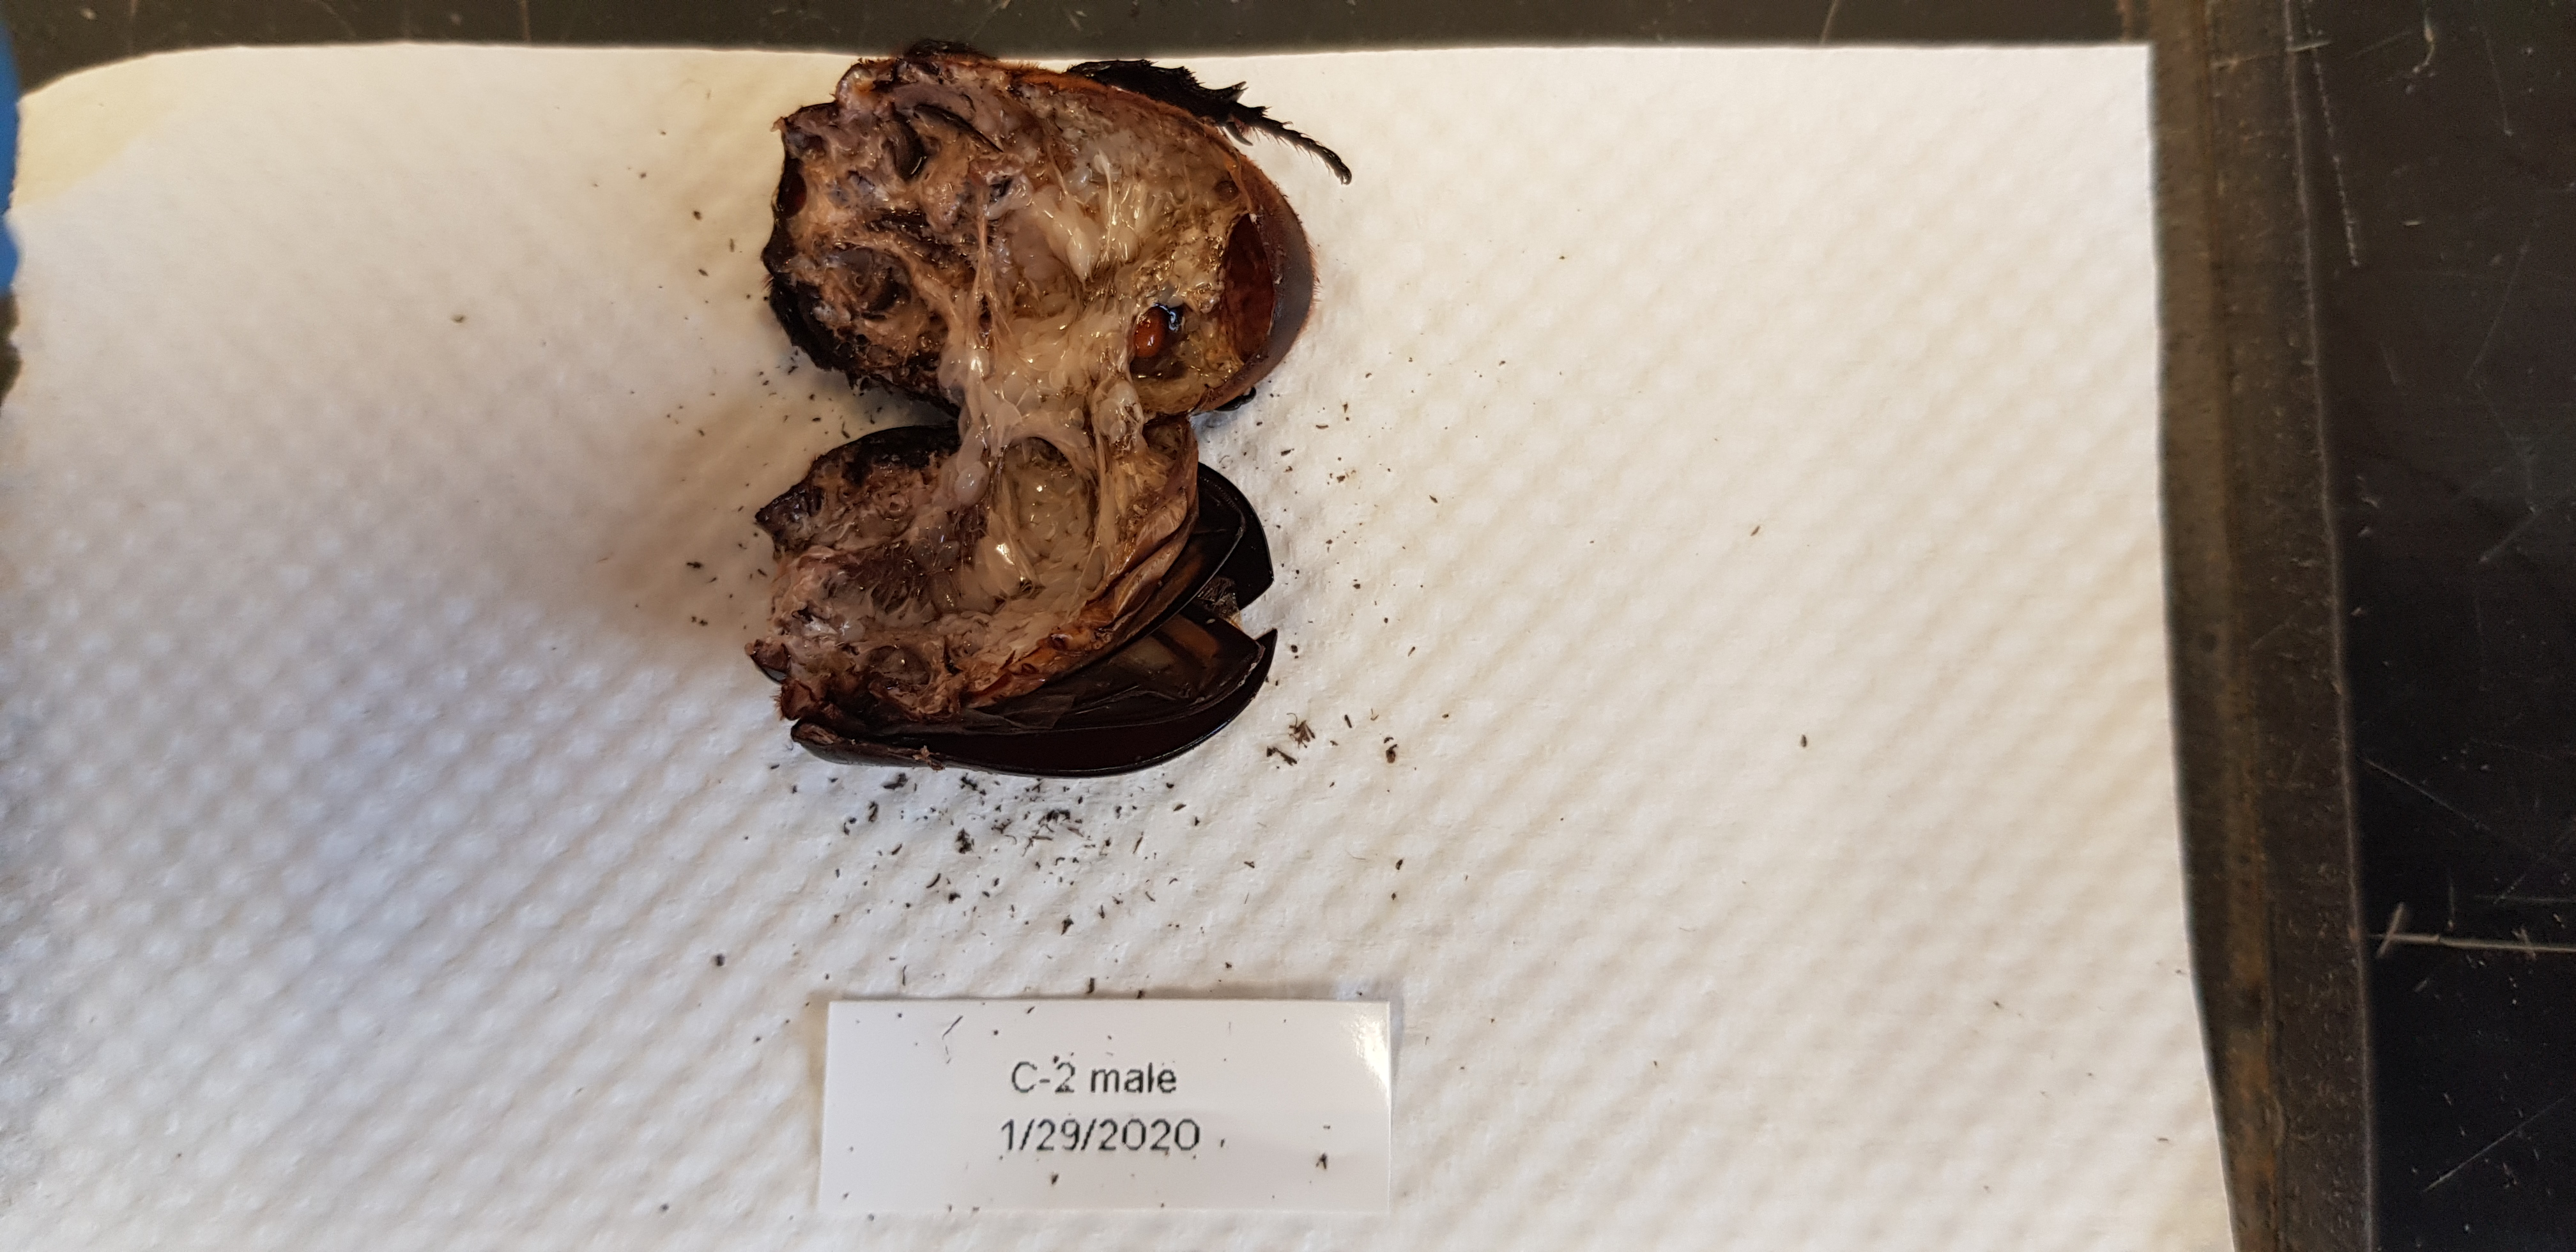
\includegraphics[width=\textwidth]{pm-images/20200129_145244.jpg}
\caption{\textbf{C2m} jar\_id                                  C2
sex                                      m
treatment                             none
date\_treated           2019-12-26 00:00:00
date\_died              2020-01-29 00:00:00
postmortem\_virus                       NaN
postmortem\_bacteria                    NaN
pm\_image\_filename      20200129\_145244.jpg
date\_end\_bioassay      2020-02-06 00:00:00
t                                       34
e                                     True
Name: 1, dtype: object}
\end{figure}
\clearpage

\begin{figure}[h!]
\centering
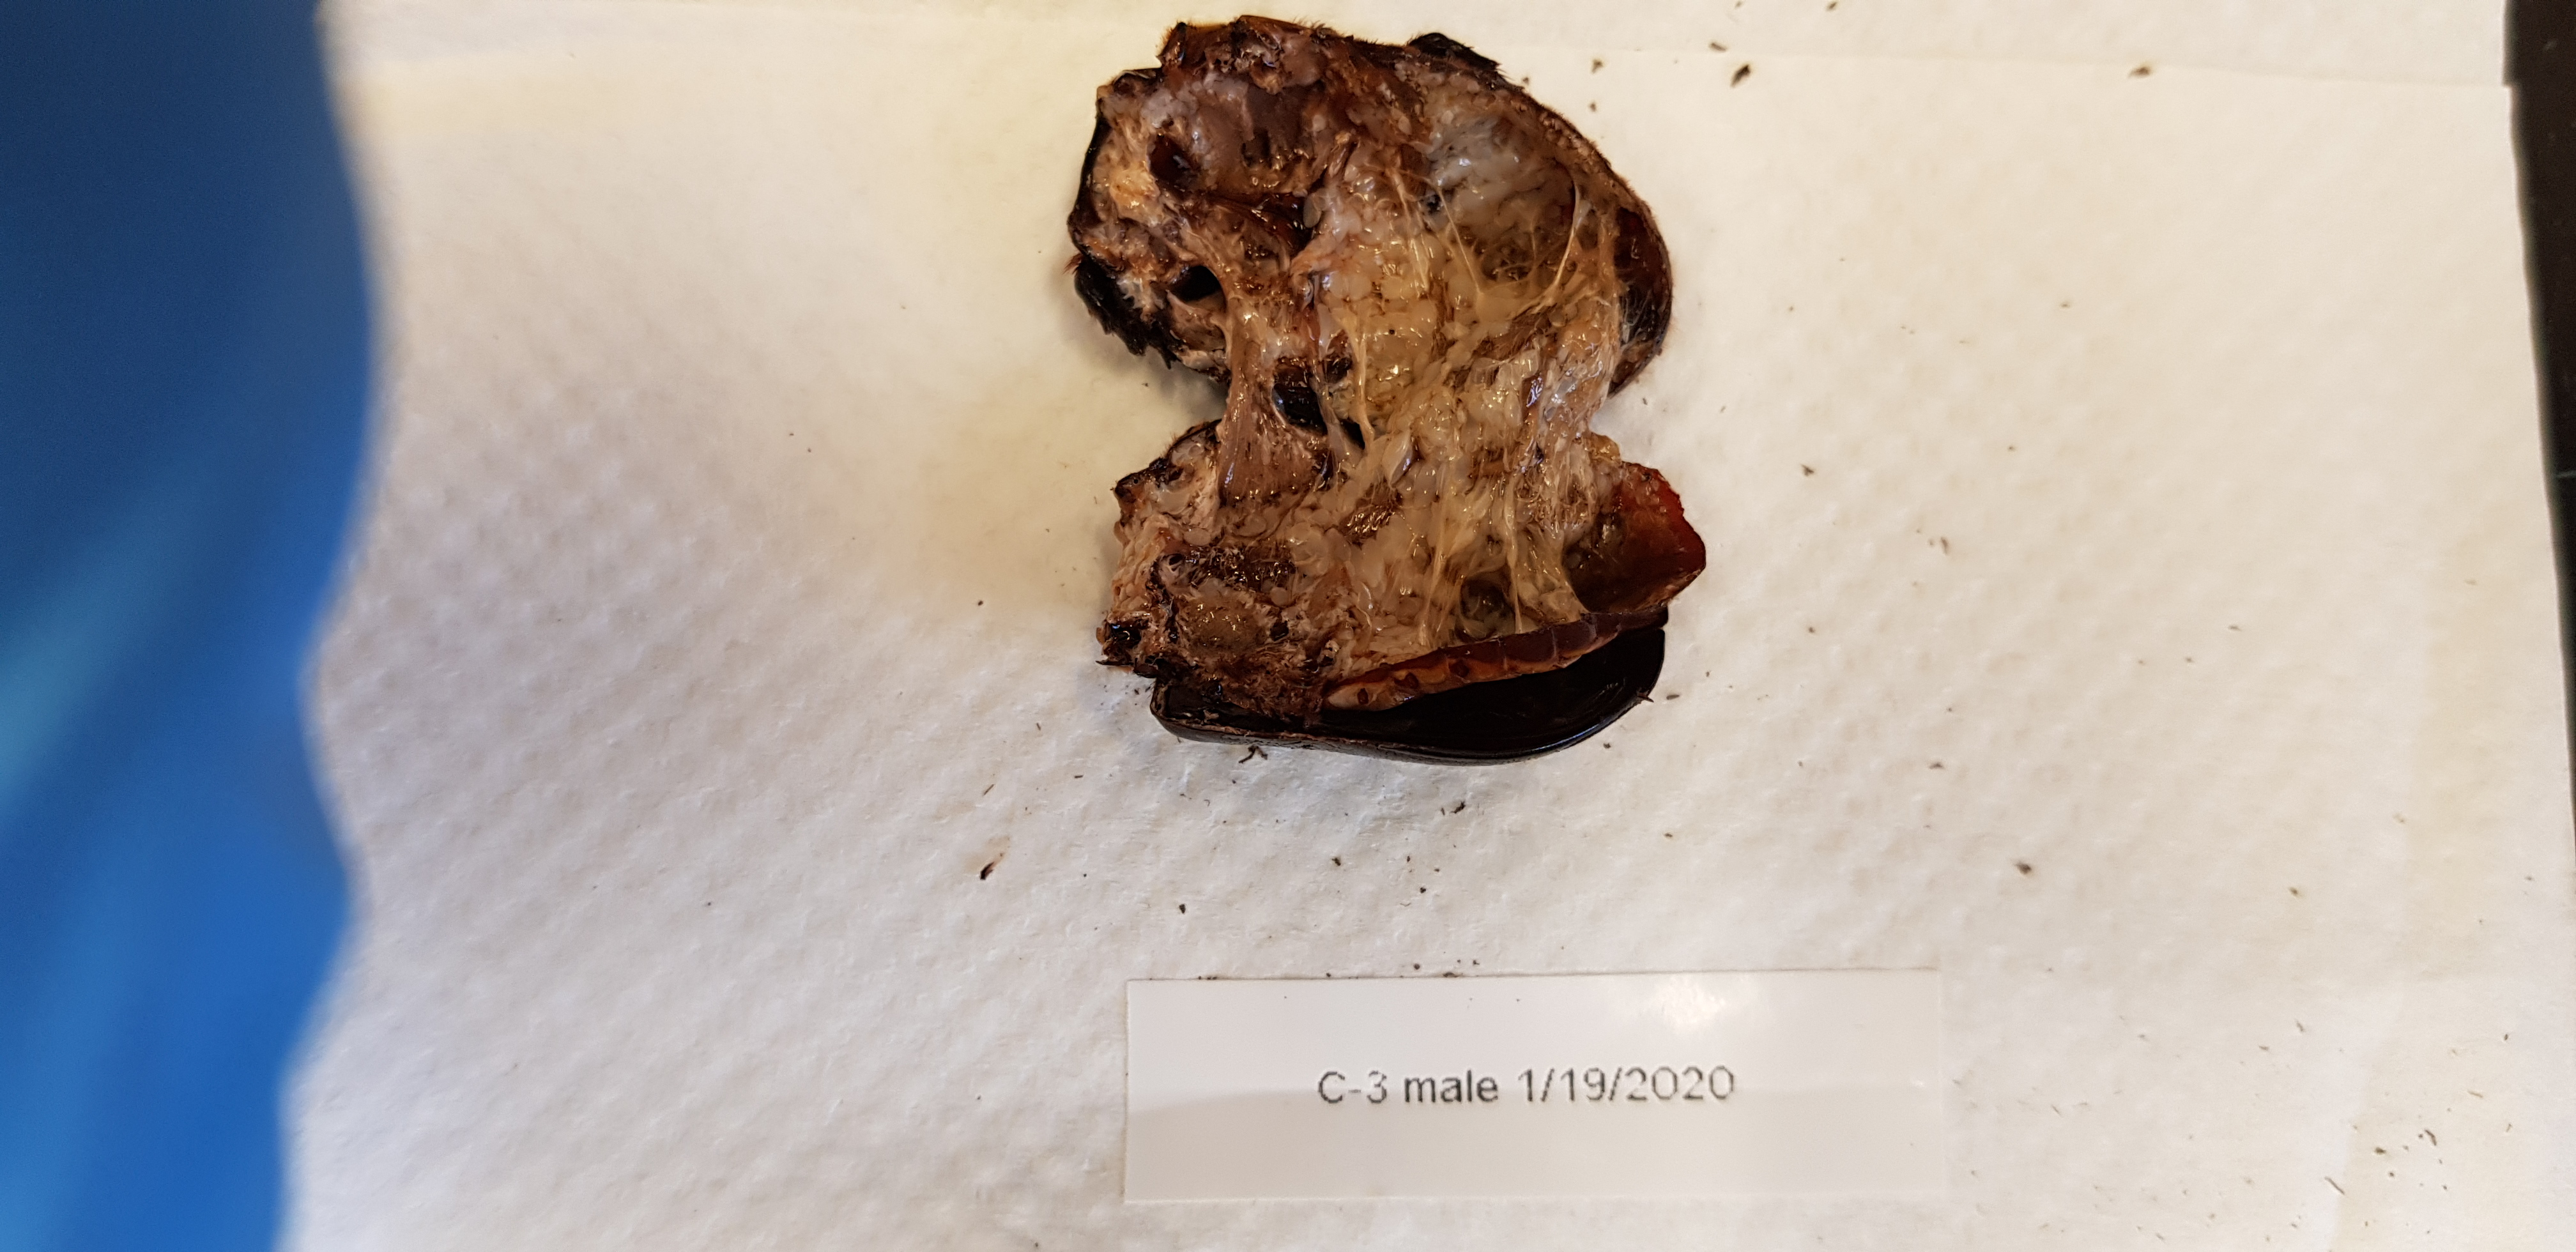
\includegraphics[width=\textwidth]{pm-images/20200119_121343.jpg}
\caption{\textbf{C3m} jar\_id                                  C3
sex                                      m
treatment                             none
date\_treated           2019-12-26 00:00:00
date\_died              2020-01-19 00:00:00
postmortem\_virus                       NaN
postmortem\_bacteria                    NaN
pm\_image\_filename      20200119\_121343.jpg
date\_end\_bioassay      2020-02-06 00:00:00
t                                       24
e                                     True
Name: 2, dtype: object}
\end{figure}
\clearpage

\begin{figure}[h!]
\centering
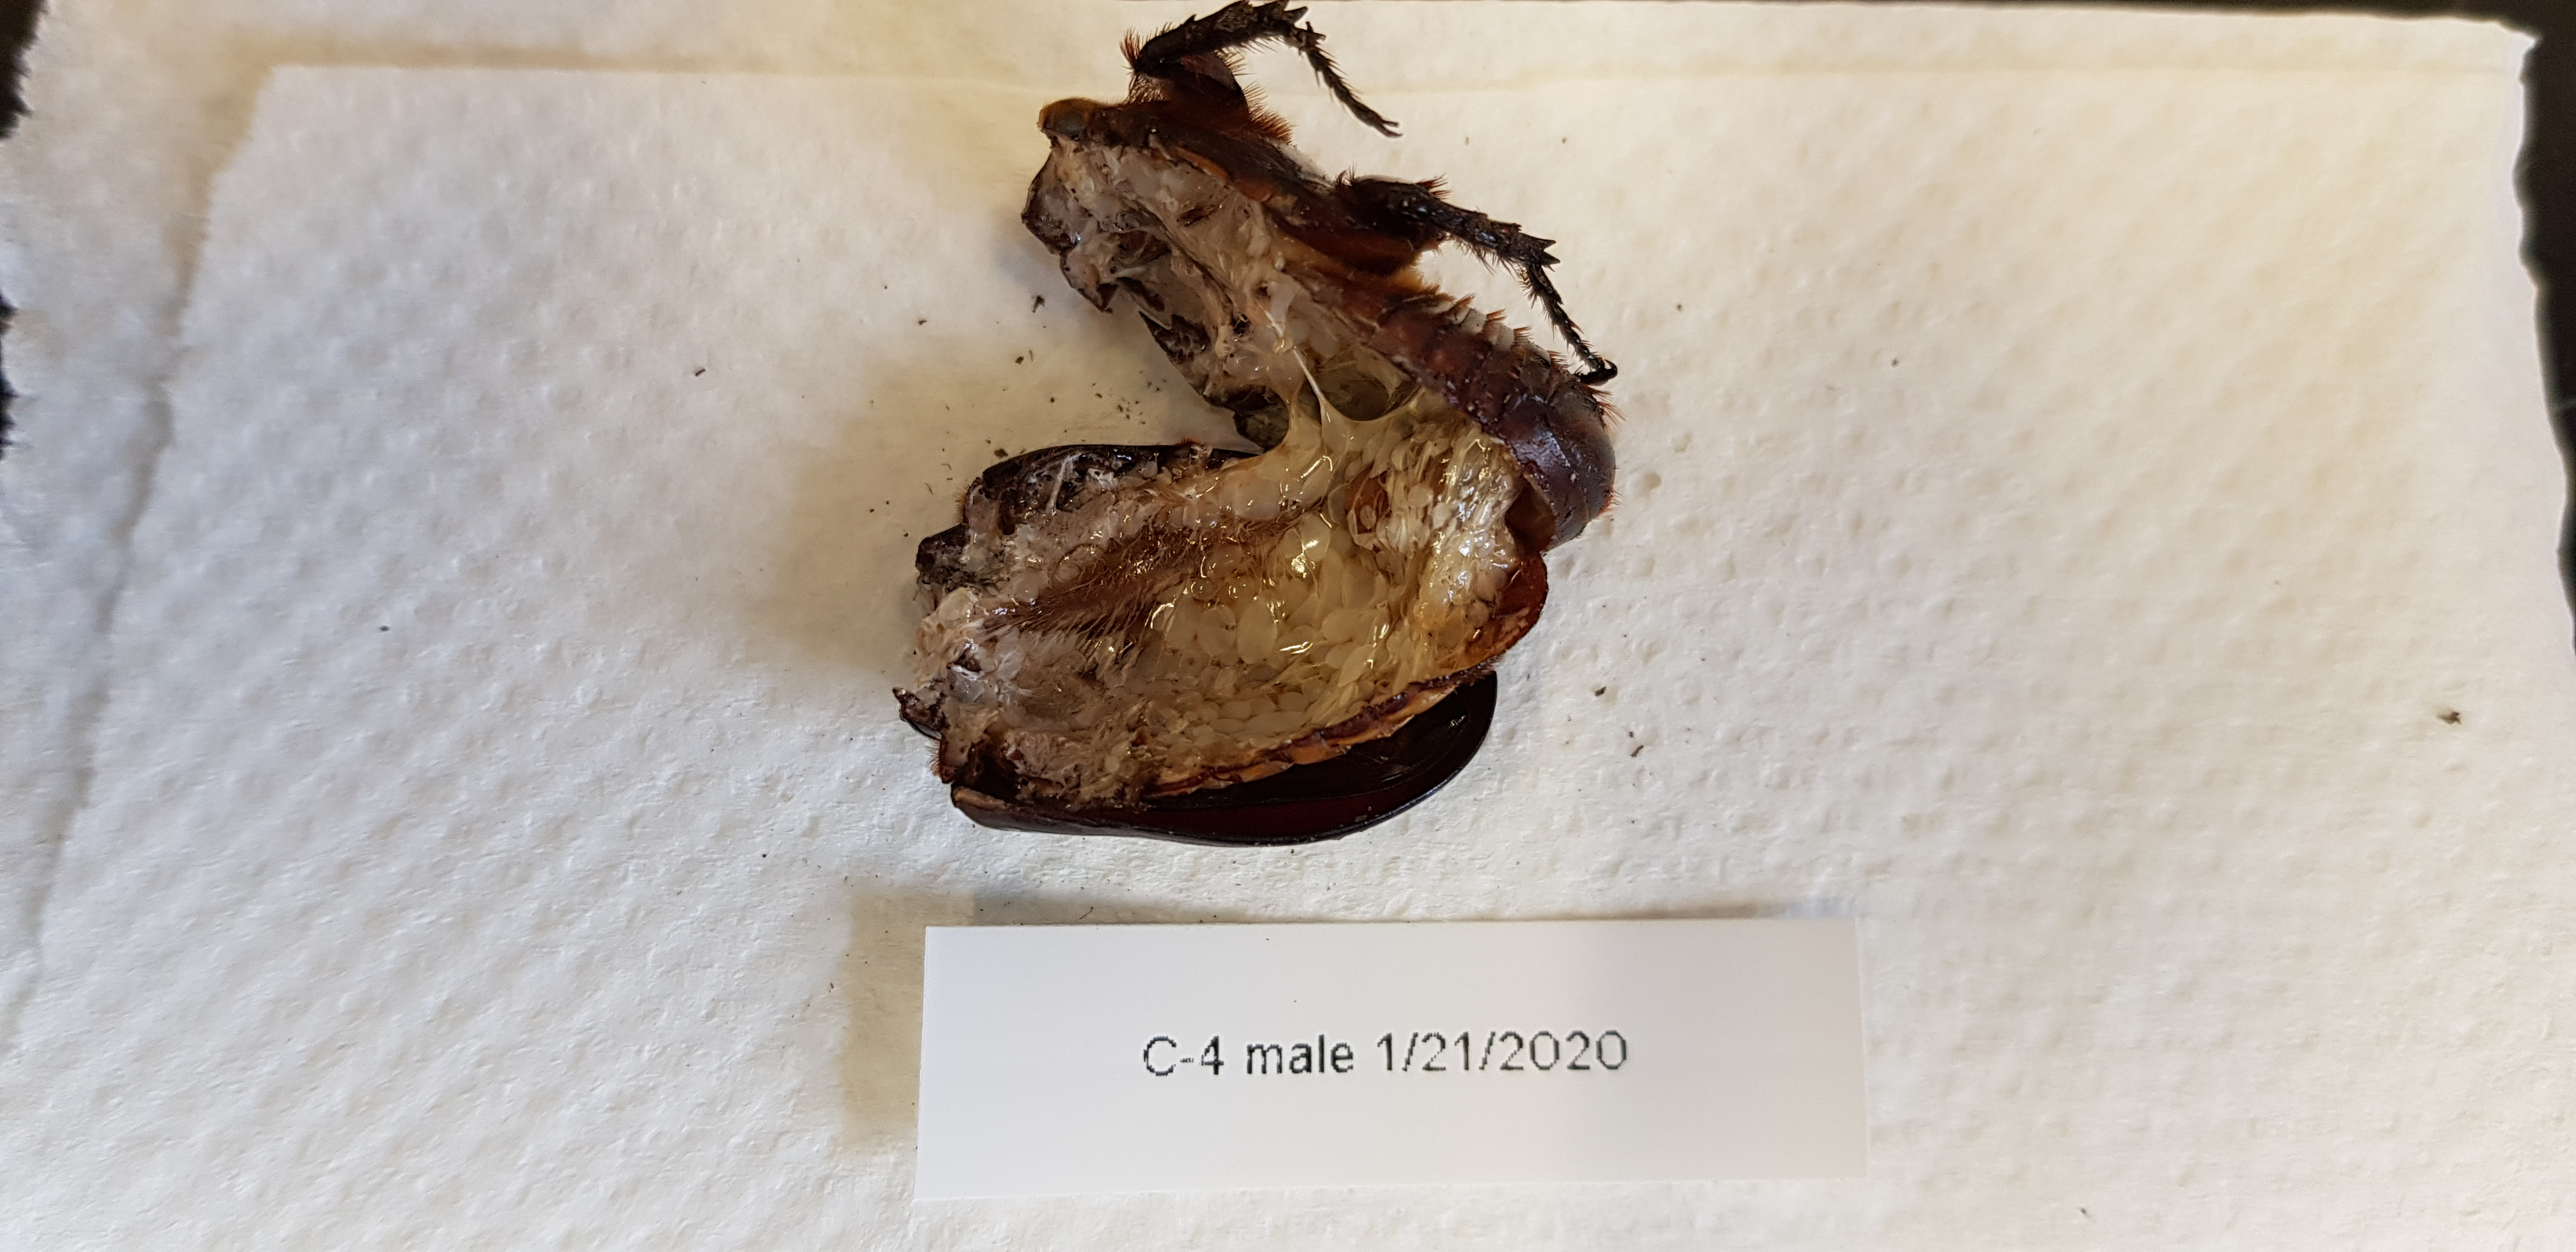
\includegraphics[width=\textwidth]{pm-images/20200121_112302.jpg}
\caption{\textbf{C4m} jar\_id                                  C4
sex                                      m
treatment                             none
date\_treated           2019-12-26 00:00:00
date\_died              2020-01-21 00:00:00
postmortem\_virus                       NaN
postmortem\_bacteria                    NaN
pm\_image\_filename      20200121\_112302.jpg
date\_end\_bioassay      2020-02-06 00:00:00
t                                       26
e                                     True
Name: 3, dtype: object}
\end{figure}
\clearpage

\begin{figure}[h!]
\centering
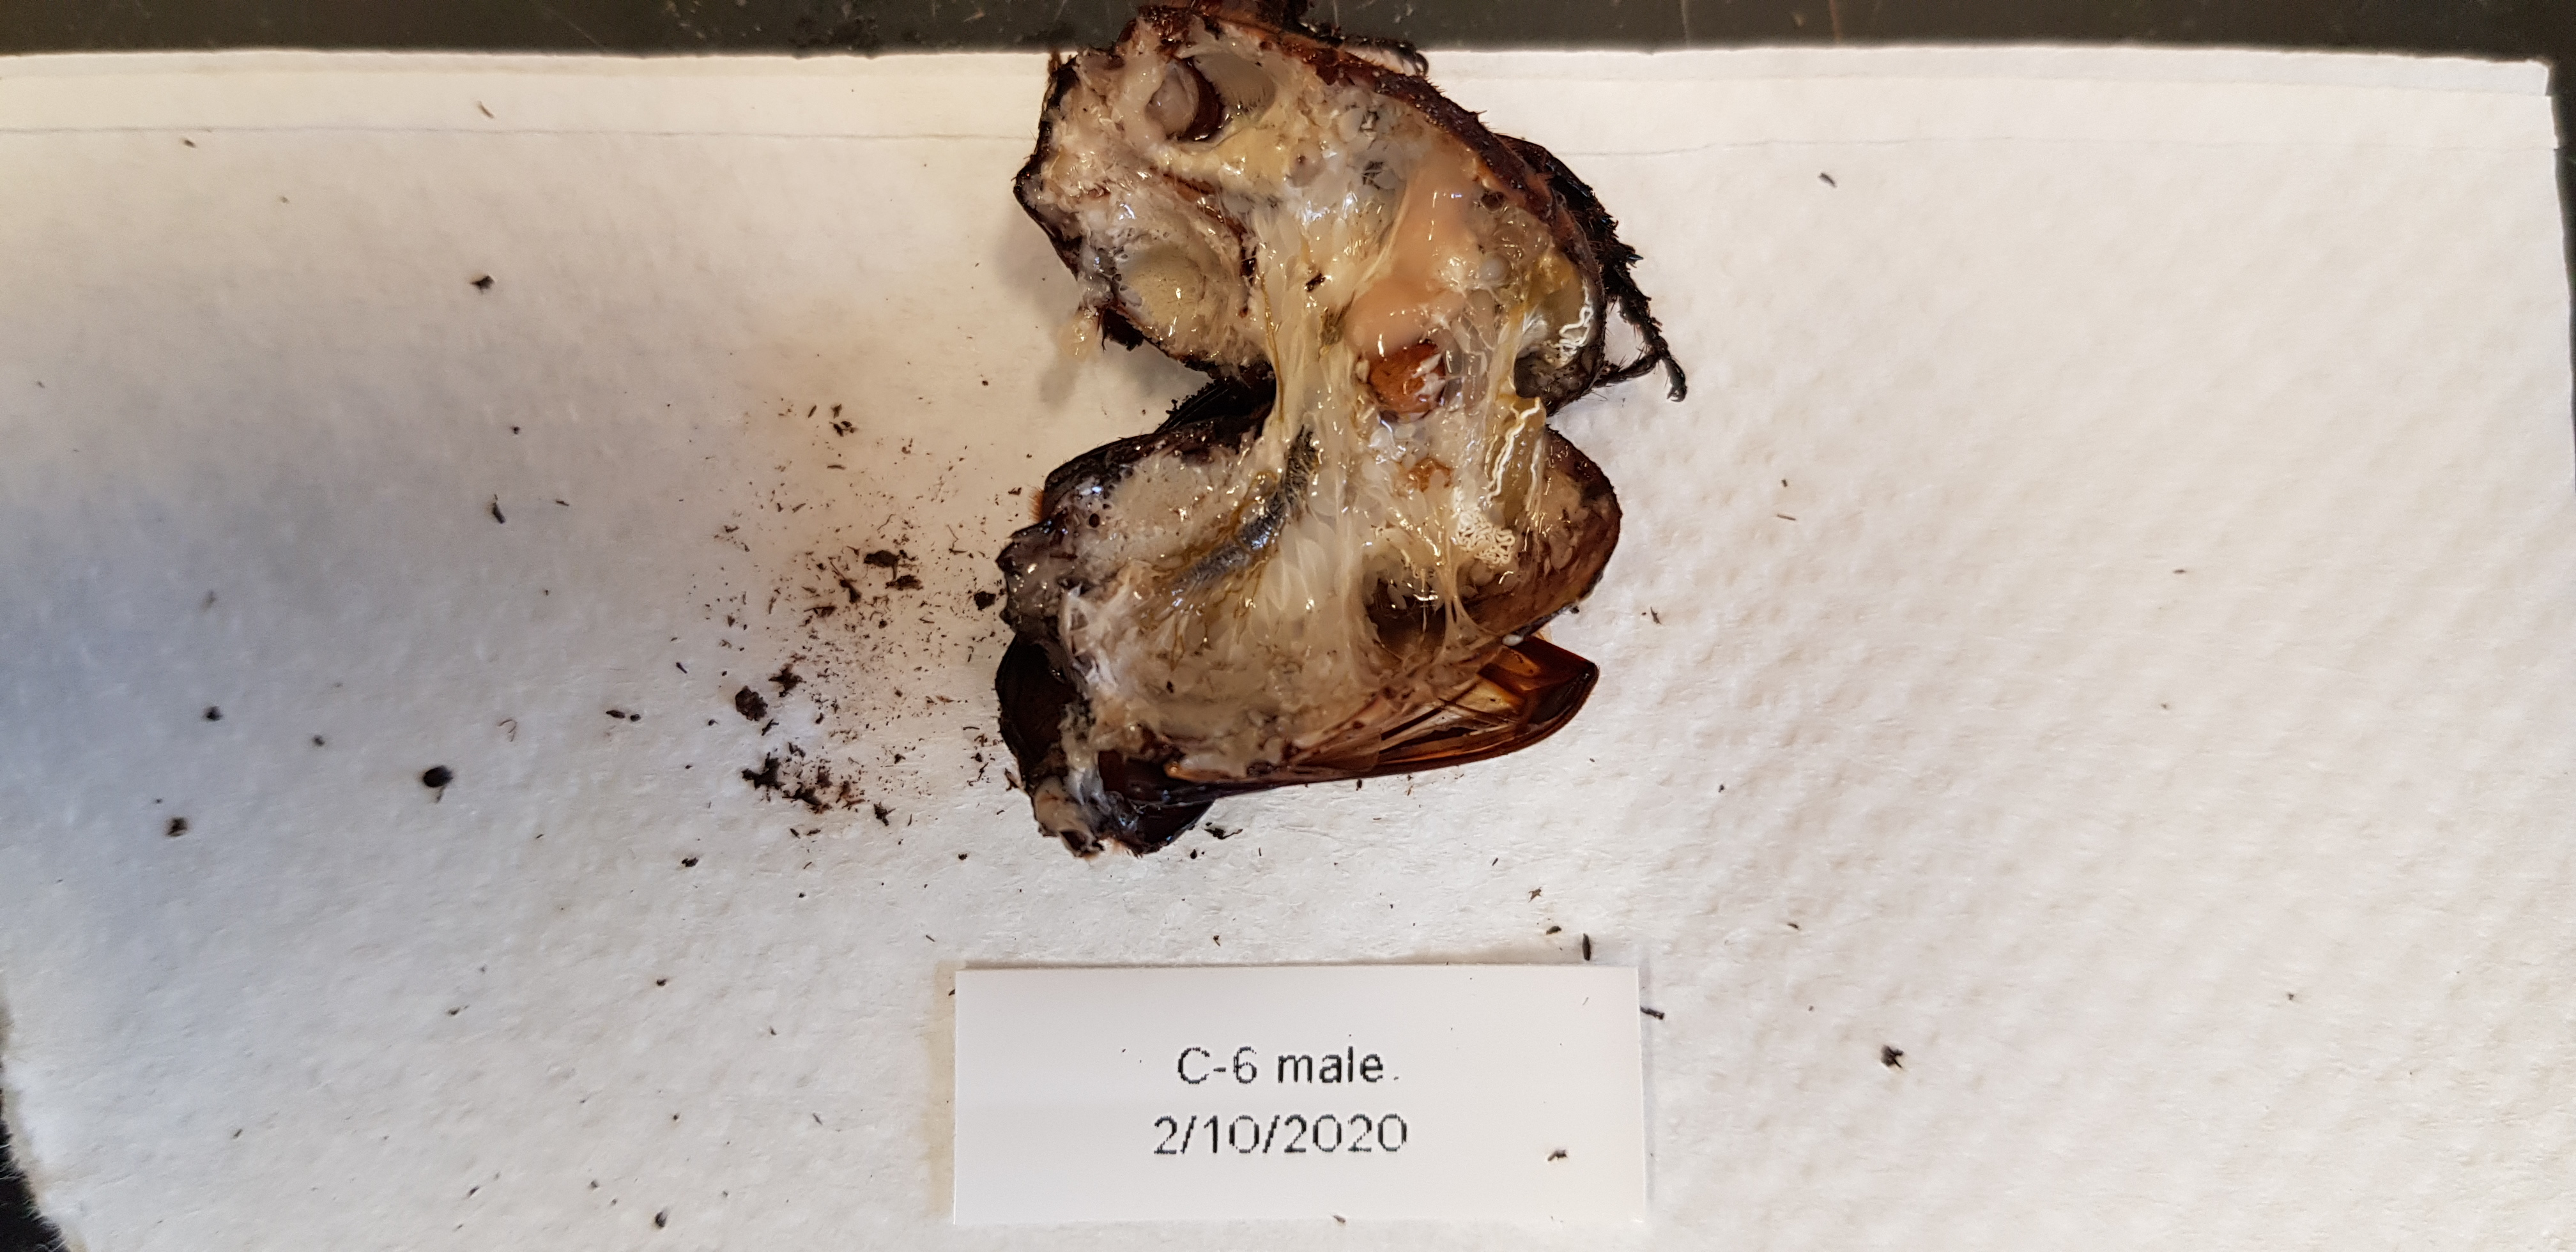
\includegraphics[width=\textwidth]{pm-images/20200210_150730.jpg}
\caption{\textbf{C6m} jar\_id                                  C6
sex                                      m
treatment                             none
date\_treated           2019-12-27 00:00:00
date\_died                              NaT
postmortem\_virus                       NaN
postmortem\_bacteria                    NaN
pm\_image\_filename      20200210\_150730.jpg
date\_end\_bioassay      2020-02-06 00:00:00
t                                       41
e                                    False
Name: 5, dtype: object}
\end{figure}
\clearpage

\begin{figure}[h!]
\centering
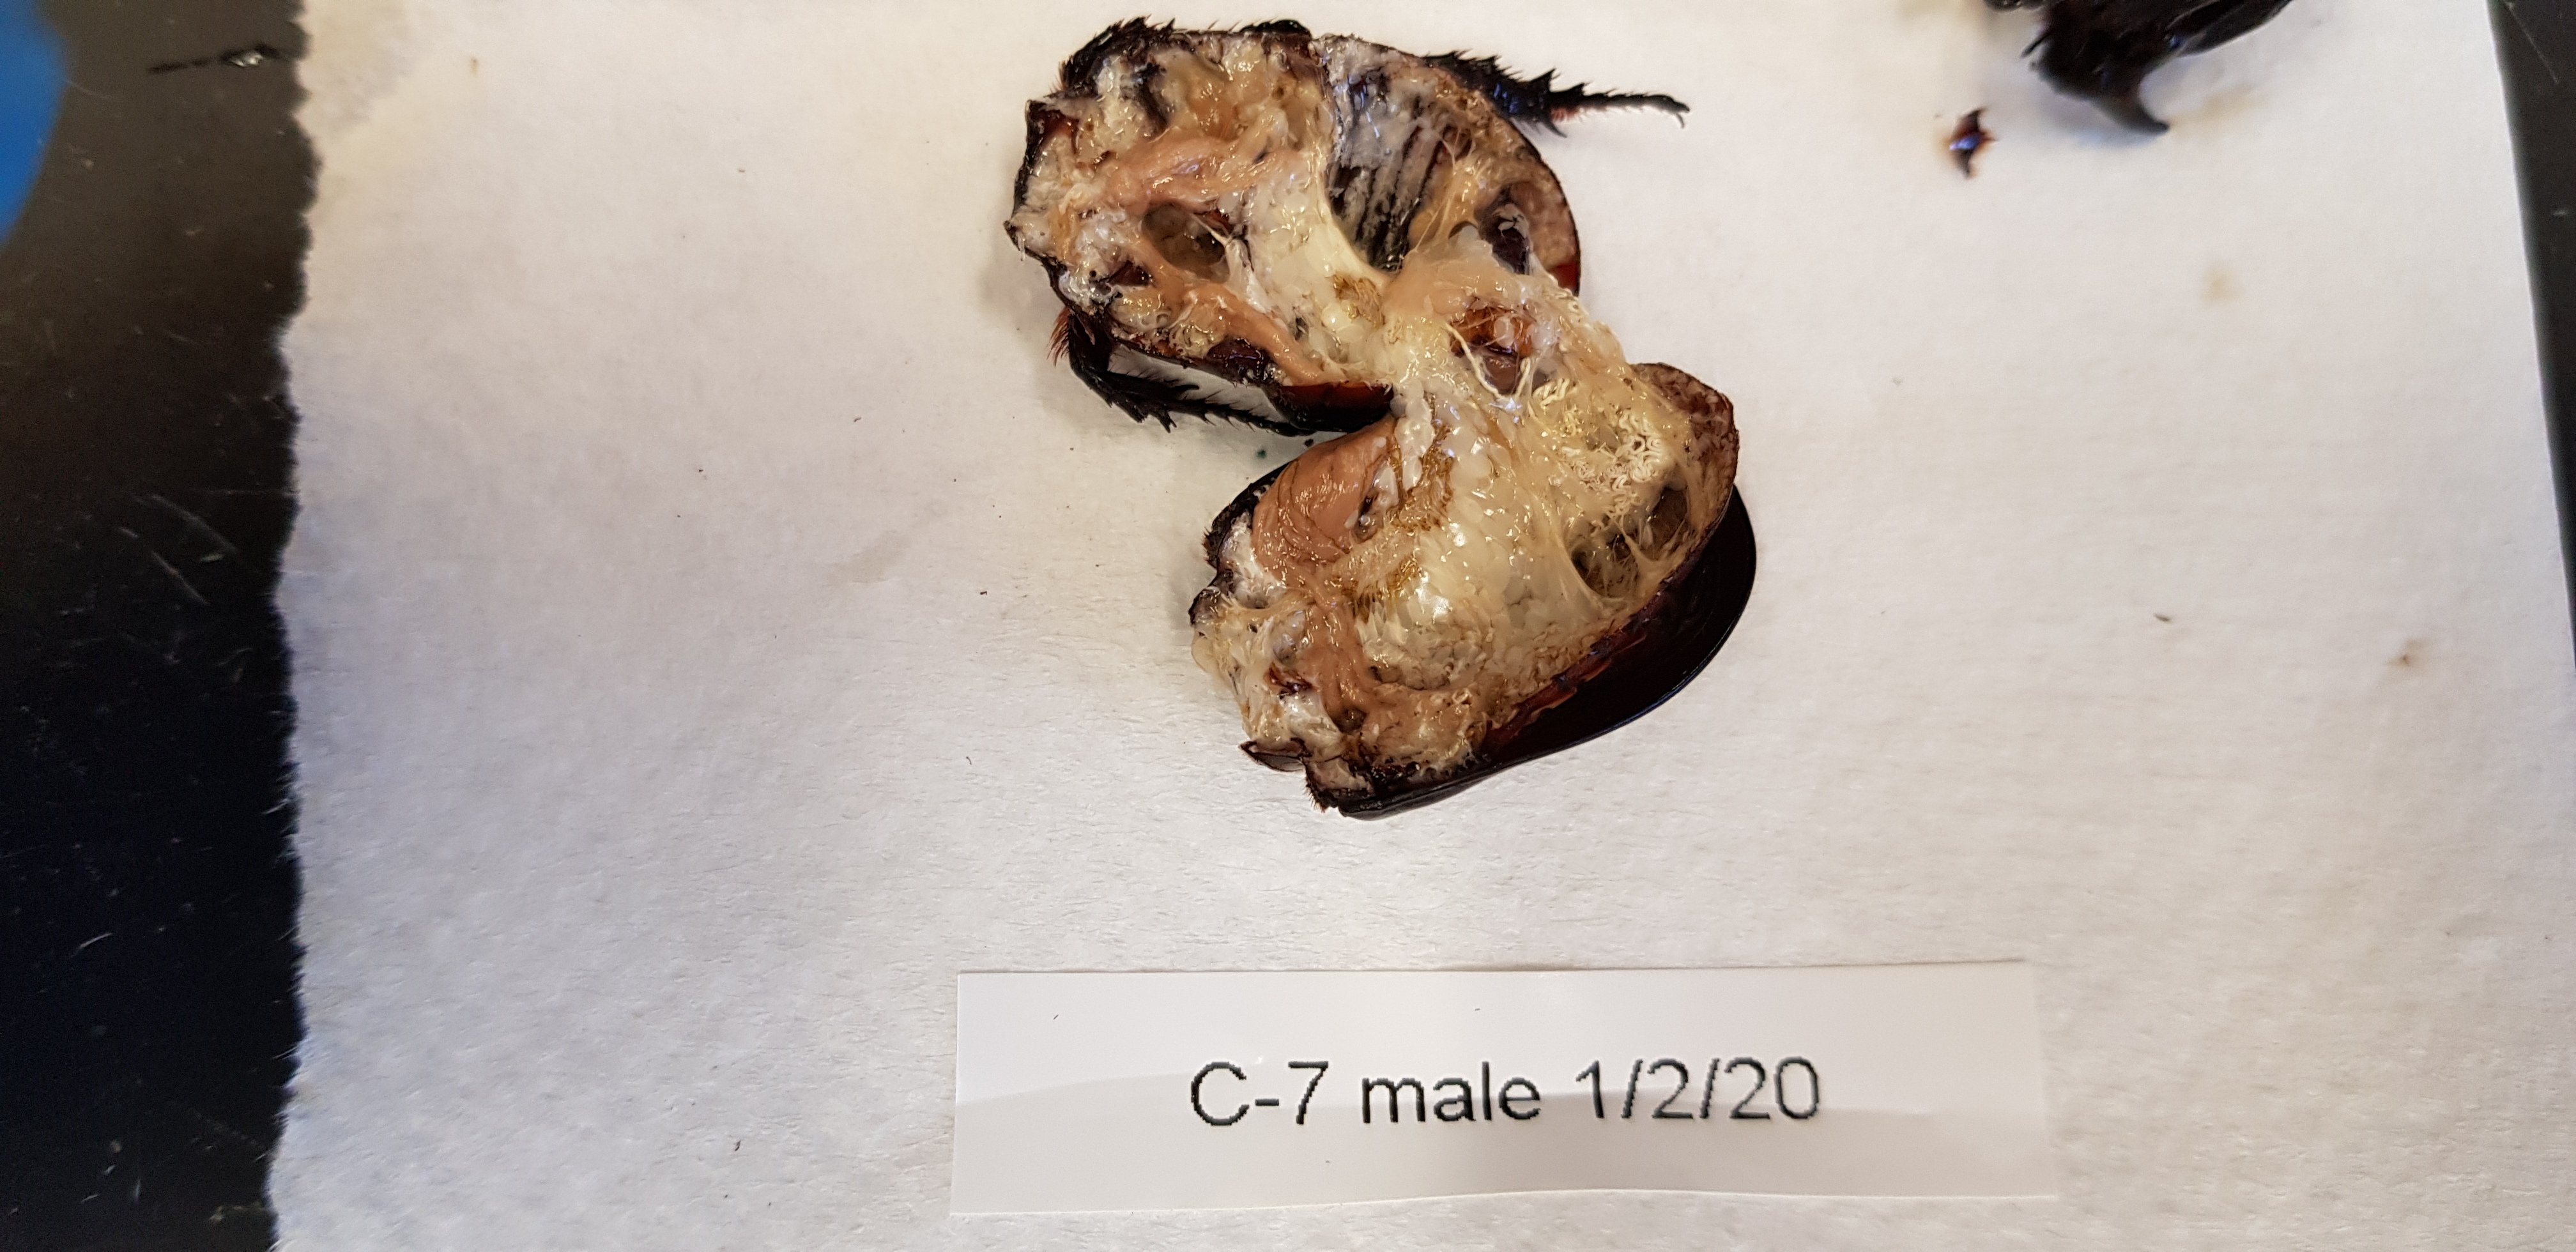
\includegraphics[width=\textwidth]{pm-images/20200102_112827.jpg}
\caption{\textbf{C7m} jar\_id                                  C7
sex                                      m
treatment                             none
date\_treated           2019-12-27 00:00:00
date\_died              2020-01-02 00:00:00
postmortem\_virus                       NaN
postmortem\_bacteria                    NaN
pm\_image\_filename      20200102\_112827.jpg
date\_end\_bioassay      2020-02-06 00:00:00
t                                        6
e                                     True
Name: 6, dtype: object}
\end{figure}
\clearpage

\begin{figure}[h!]
\centering
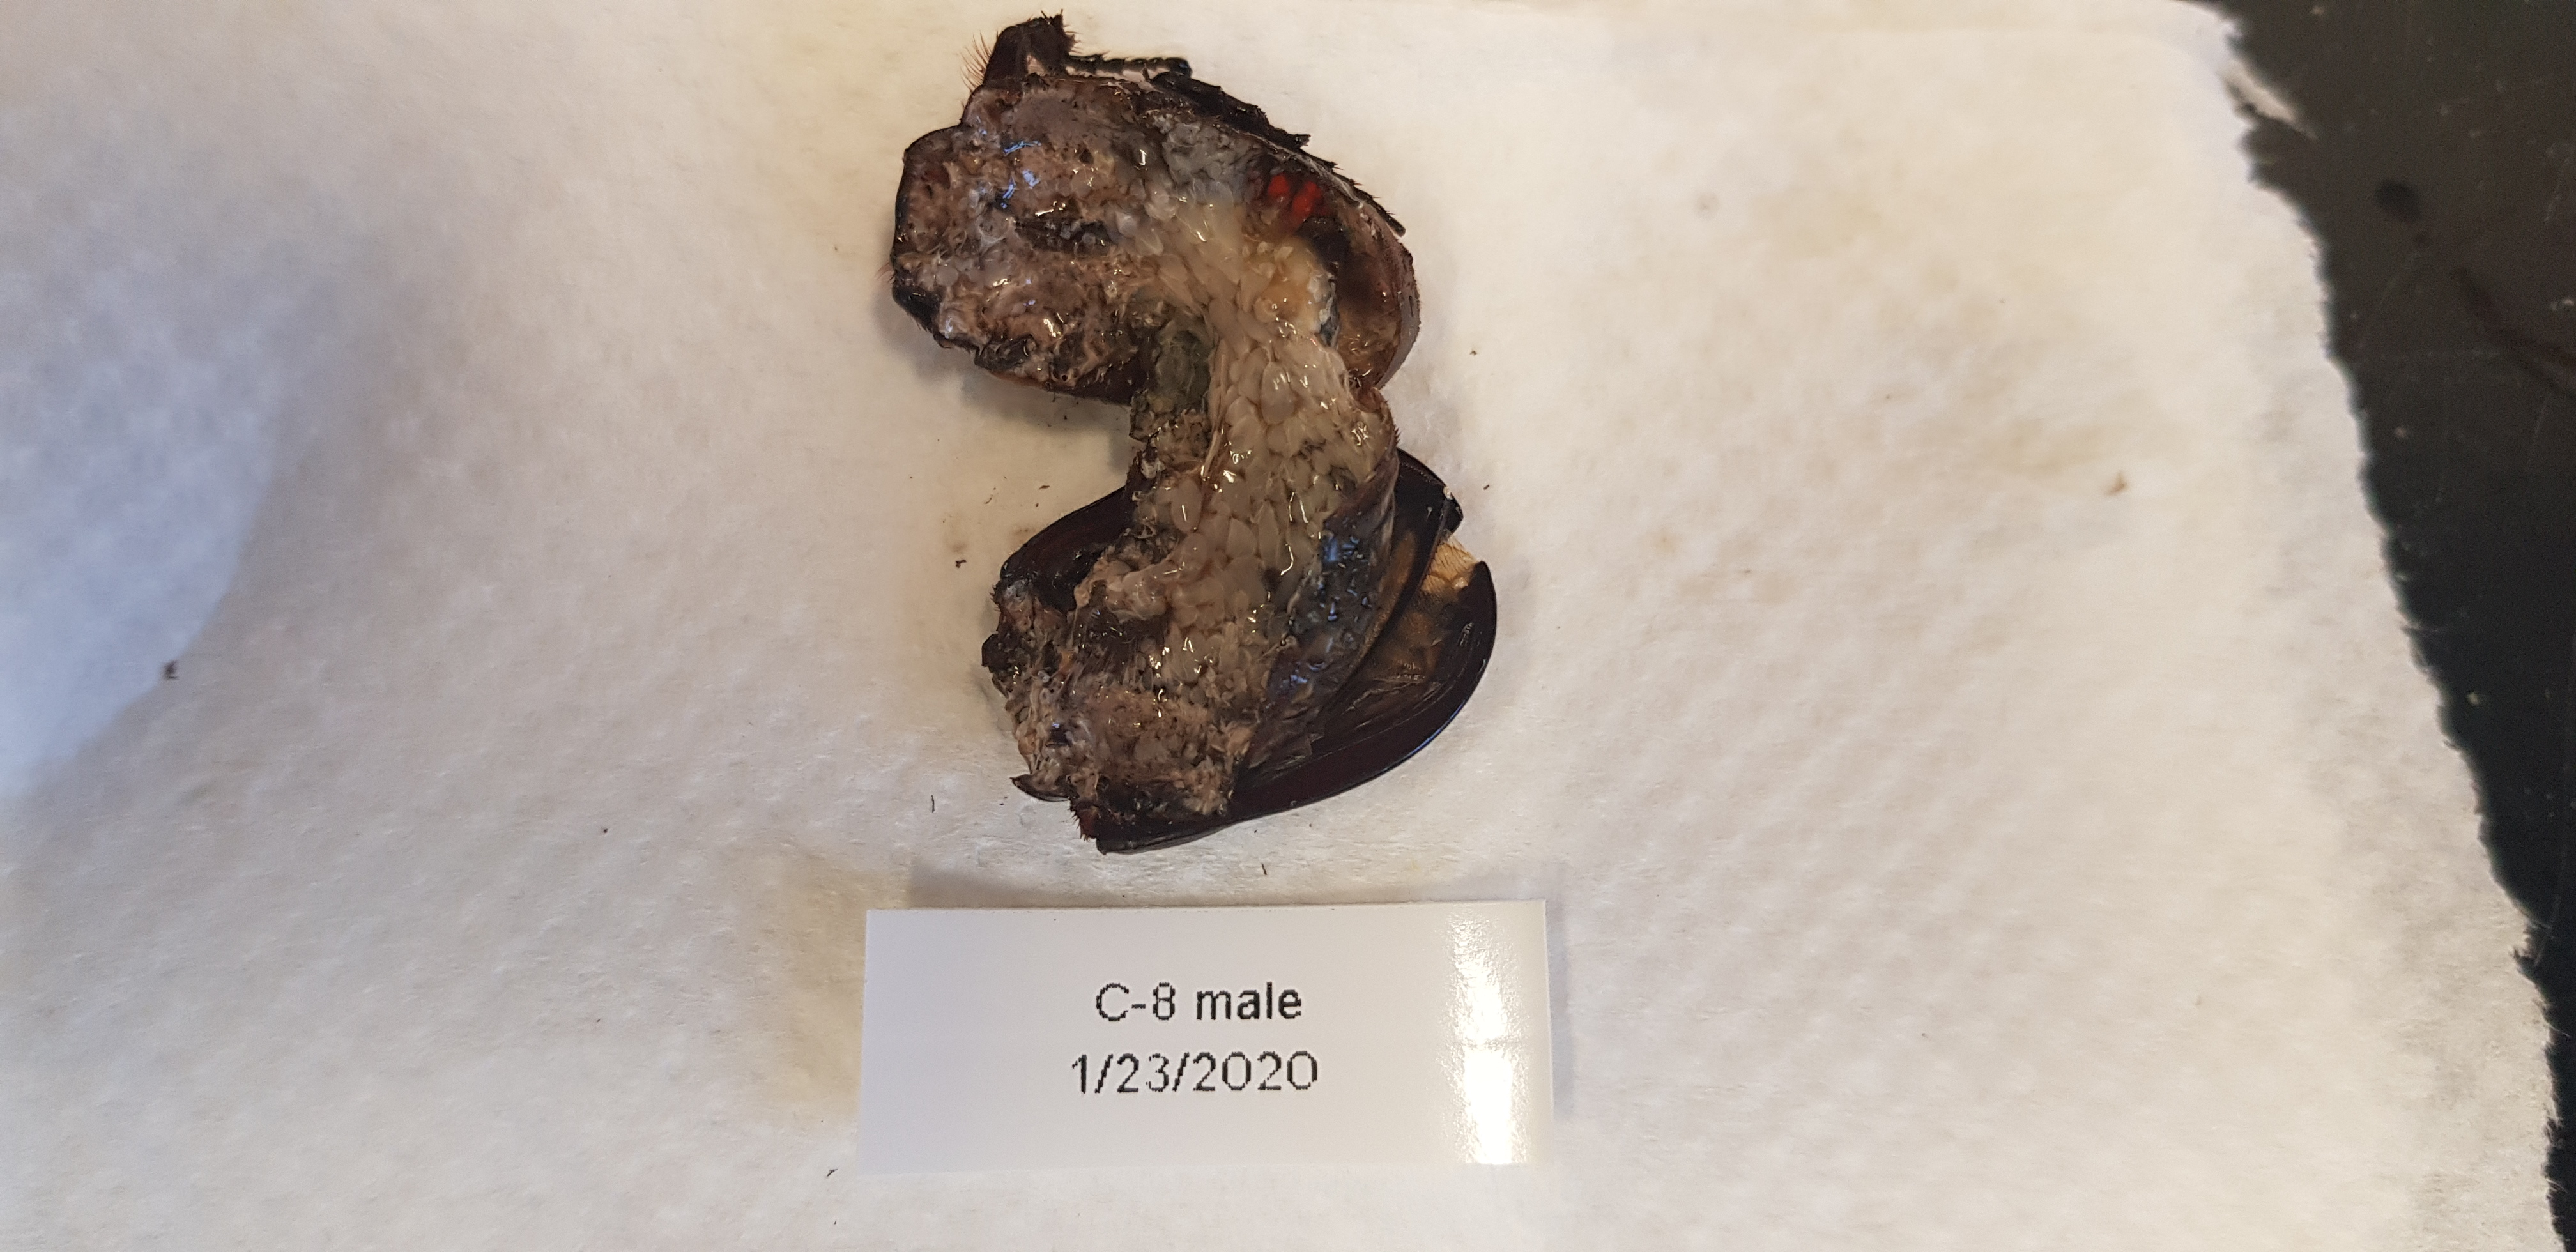
\includegraphics[width=\textwidth]{pm-images/20200123_163747.jpg}
\caption{\textbf{C8m} jar\_id                                  C8
sex                                      m
treatment                             none
date\_treated           2019-12-27 00:00:00
date\_died              2020-01-23 00:00:00
postmortem\_virus                       NaN
postmortem\_bacteria                      1
pm\_image\_filename      20200123\_163747.jpg
date\_end\_bioassay      2020-02-06 00:00:00
t                                       27
e                                     True
Name: 7, dtype: object}
\end{figure}
\clearpage

\begin{figure}[h!]
\centering
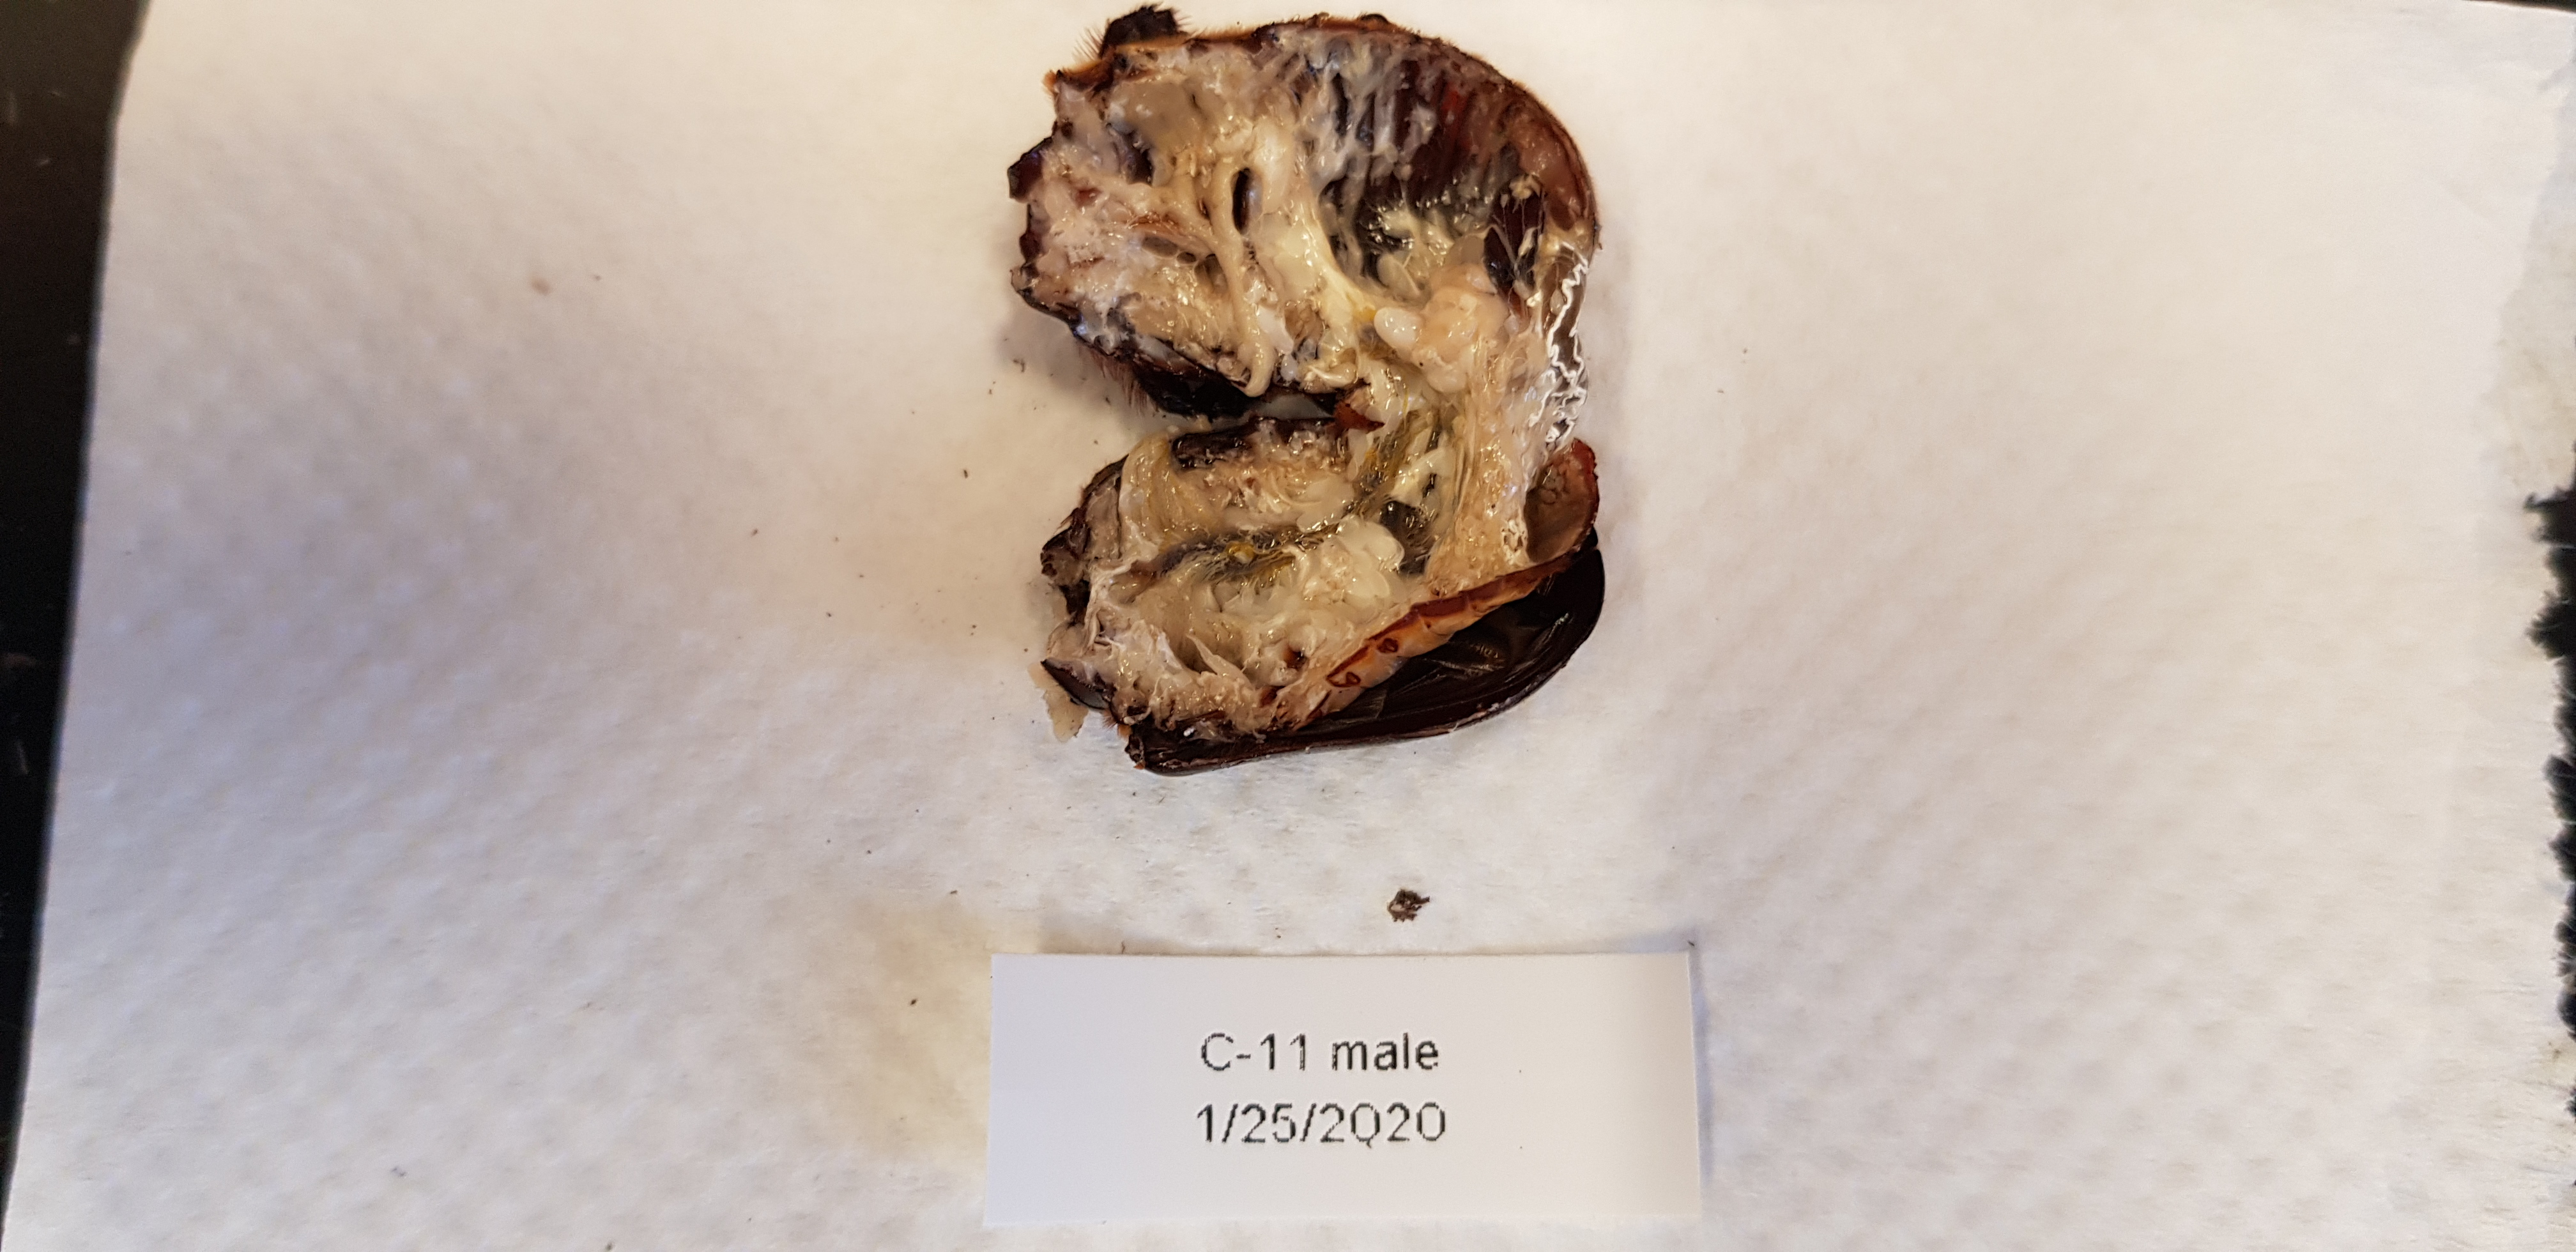
\includegraphics[width=\textwidth]{pm-images/20200125_122409.jpg}
\caption{\textbf{C11m} jar\_id                                 C11
sex                                      m
treatment                             none
date\_treated           2019-12-27 00:00:00
date\_died              2020-01-25 00:00:00
postmortem\_virus                       NaN
postmortem\_bacteria                    NaN
pm\_image\_filename      20200125\_122409.jpg
date\_end\_bioassay      2020-02-06 00:00:00
t                                       29
e                                     True
Name: 10, dtype: object}
\end{figure}
\clearpage

\begin{figure}[h!]
\centering
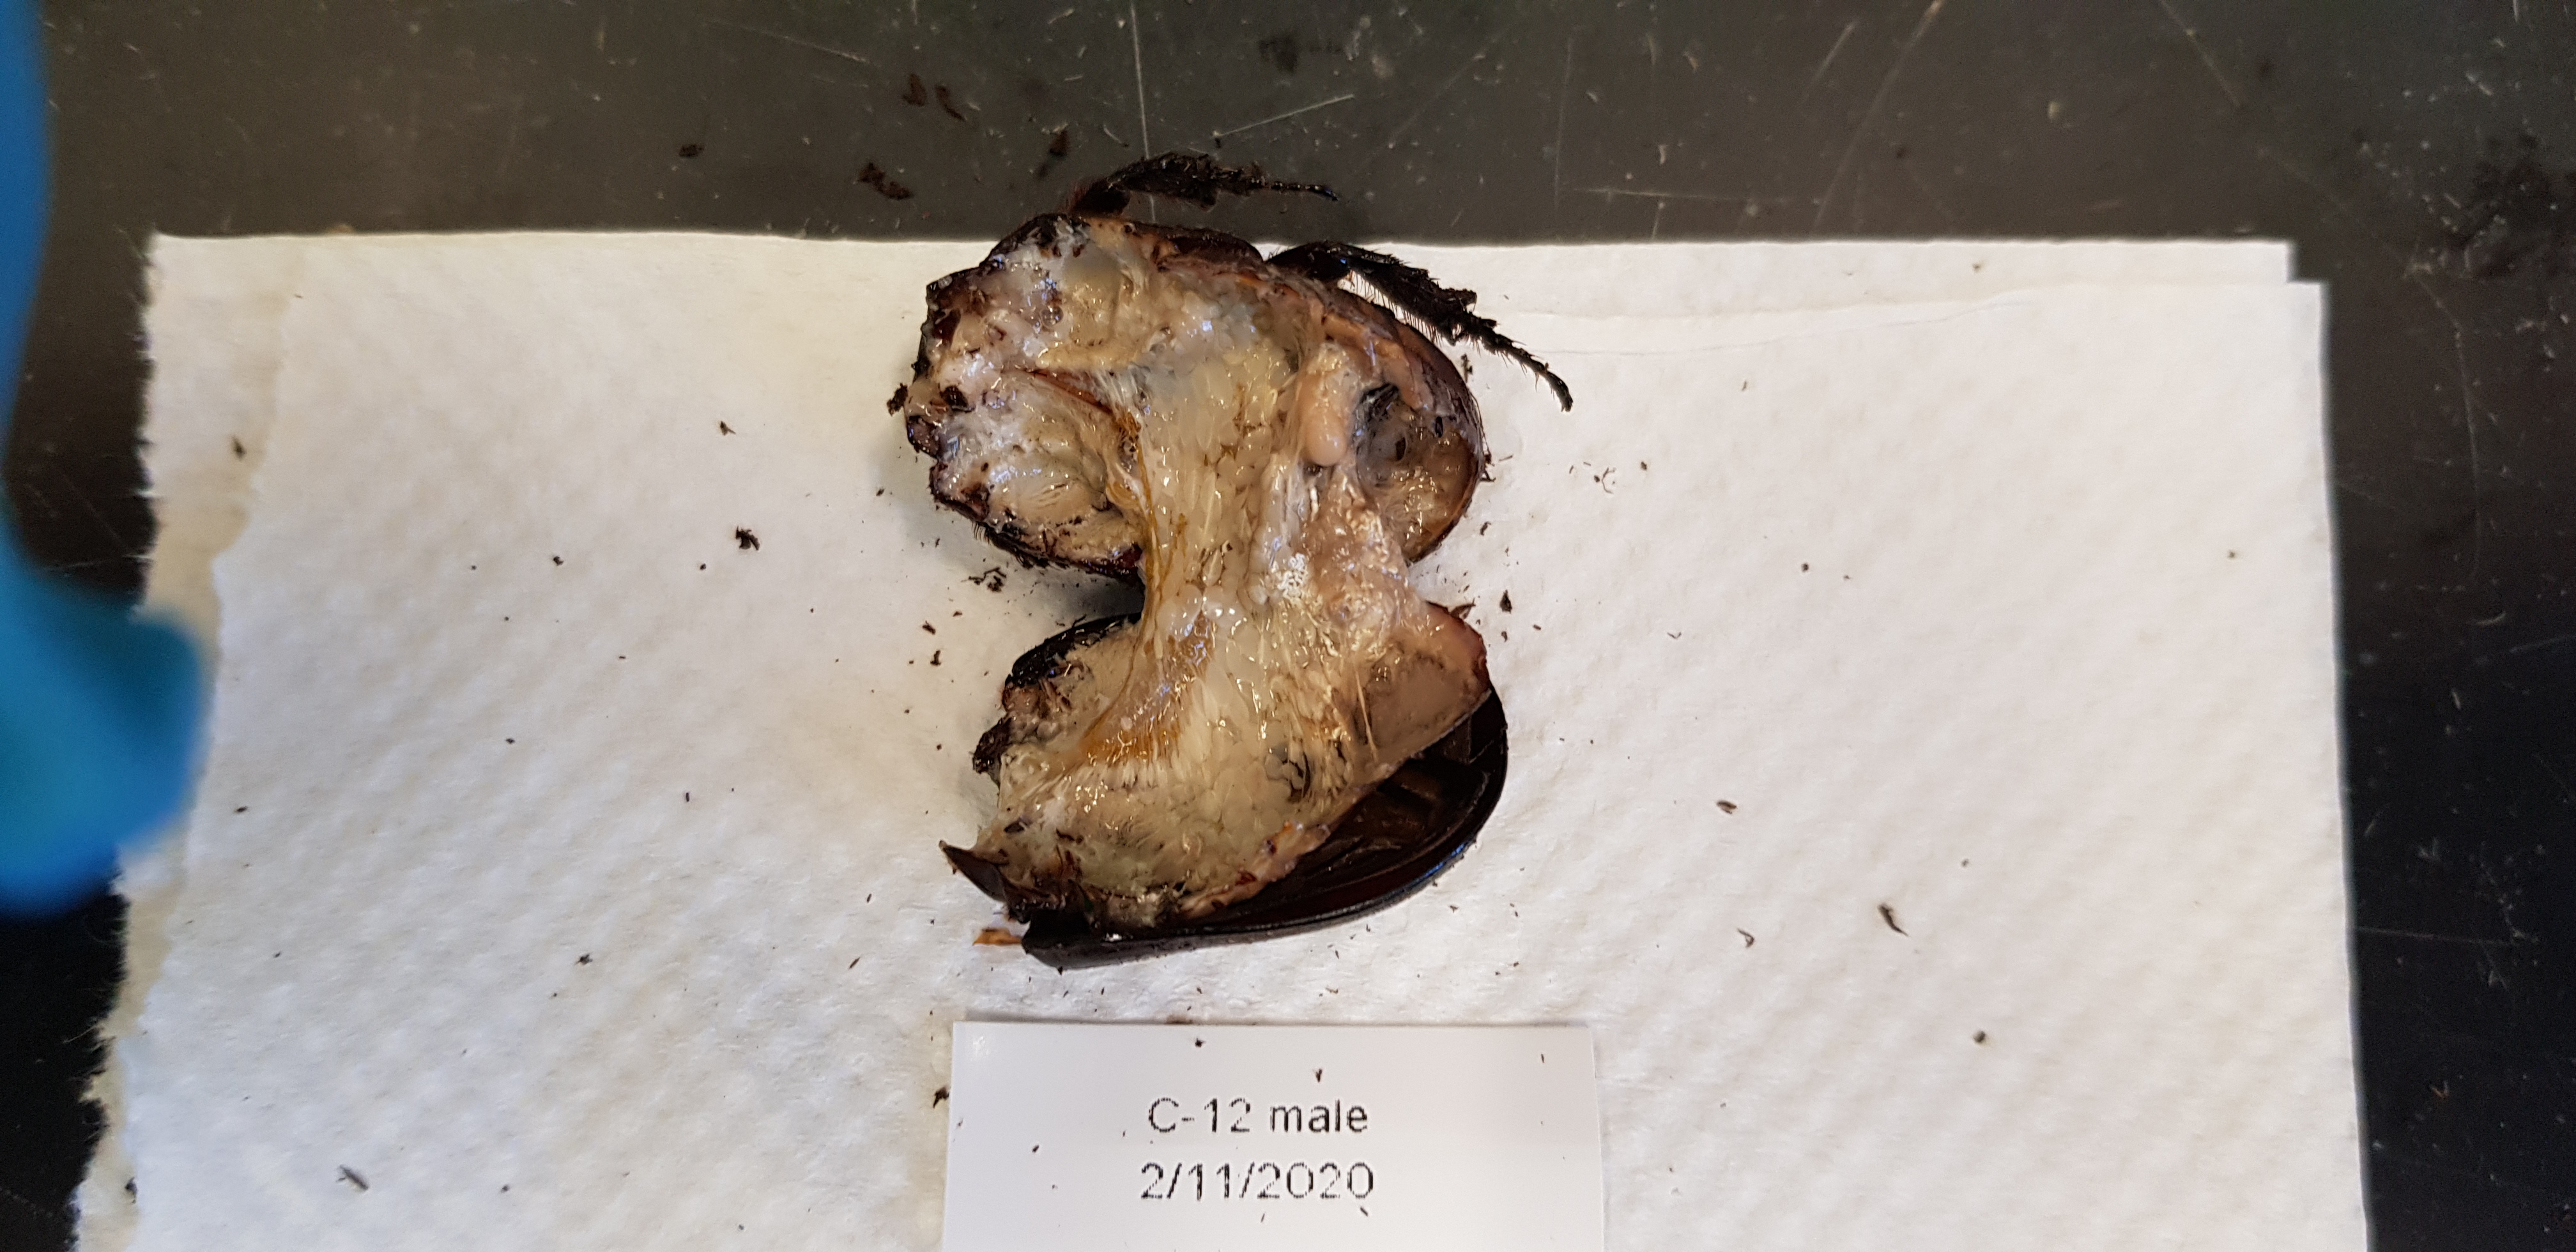
\includegraphics[width=\textwidth]{pm-images/20200211_095032.jpg}
\caption{\textbf{C12m} jar\_id                                 C12
sex                                      m
treatment                             none
date\_treated           2019-12-27 00:00:00
date\_died                              NaT
postmortem\_virus                       NaN
postmortem\_bacteria                    NaN
pm\_image\_filename      20200211\_095032.jpg
date\_end\_bioassay      2020-02-06 00:00:00
t                                       41
e                                    False
Name: 11, dtype: object}
\end{figure}
\clearpage

\begin{figure}[h!]
\centering
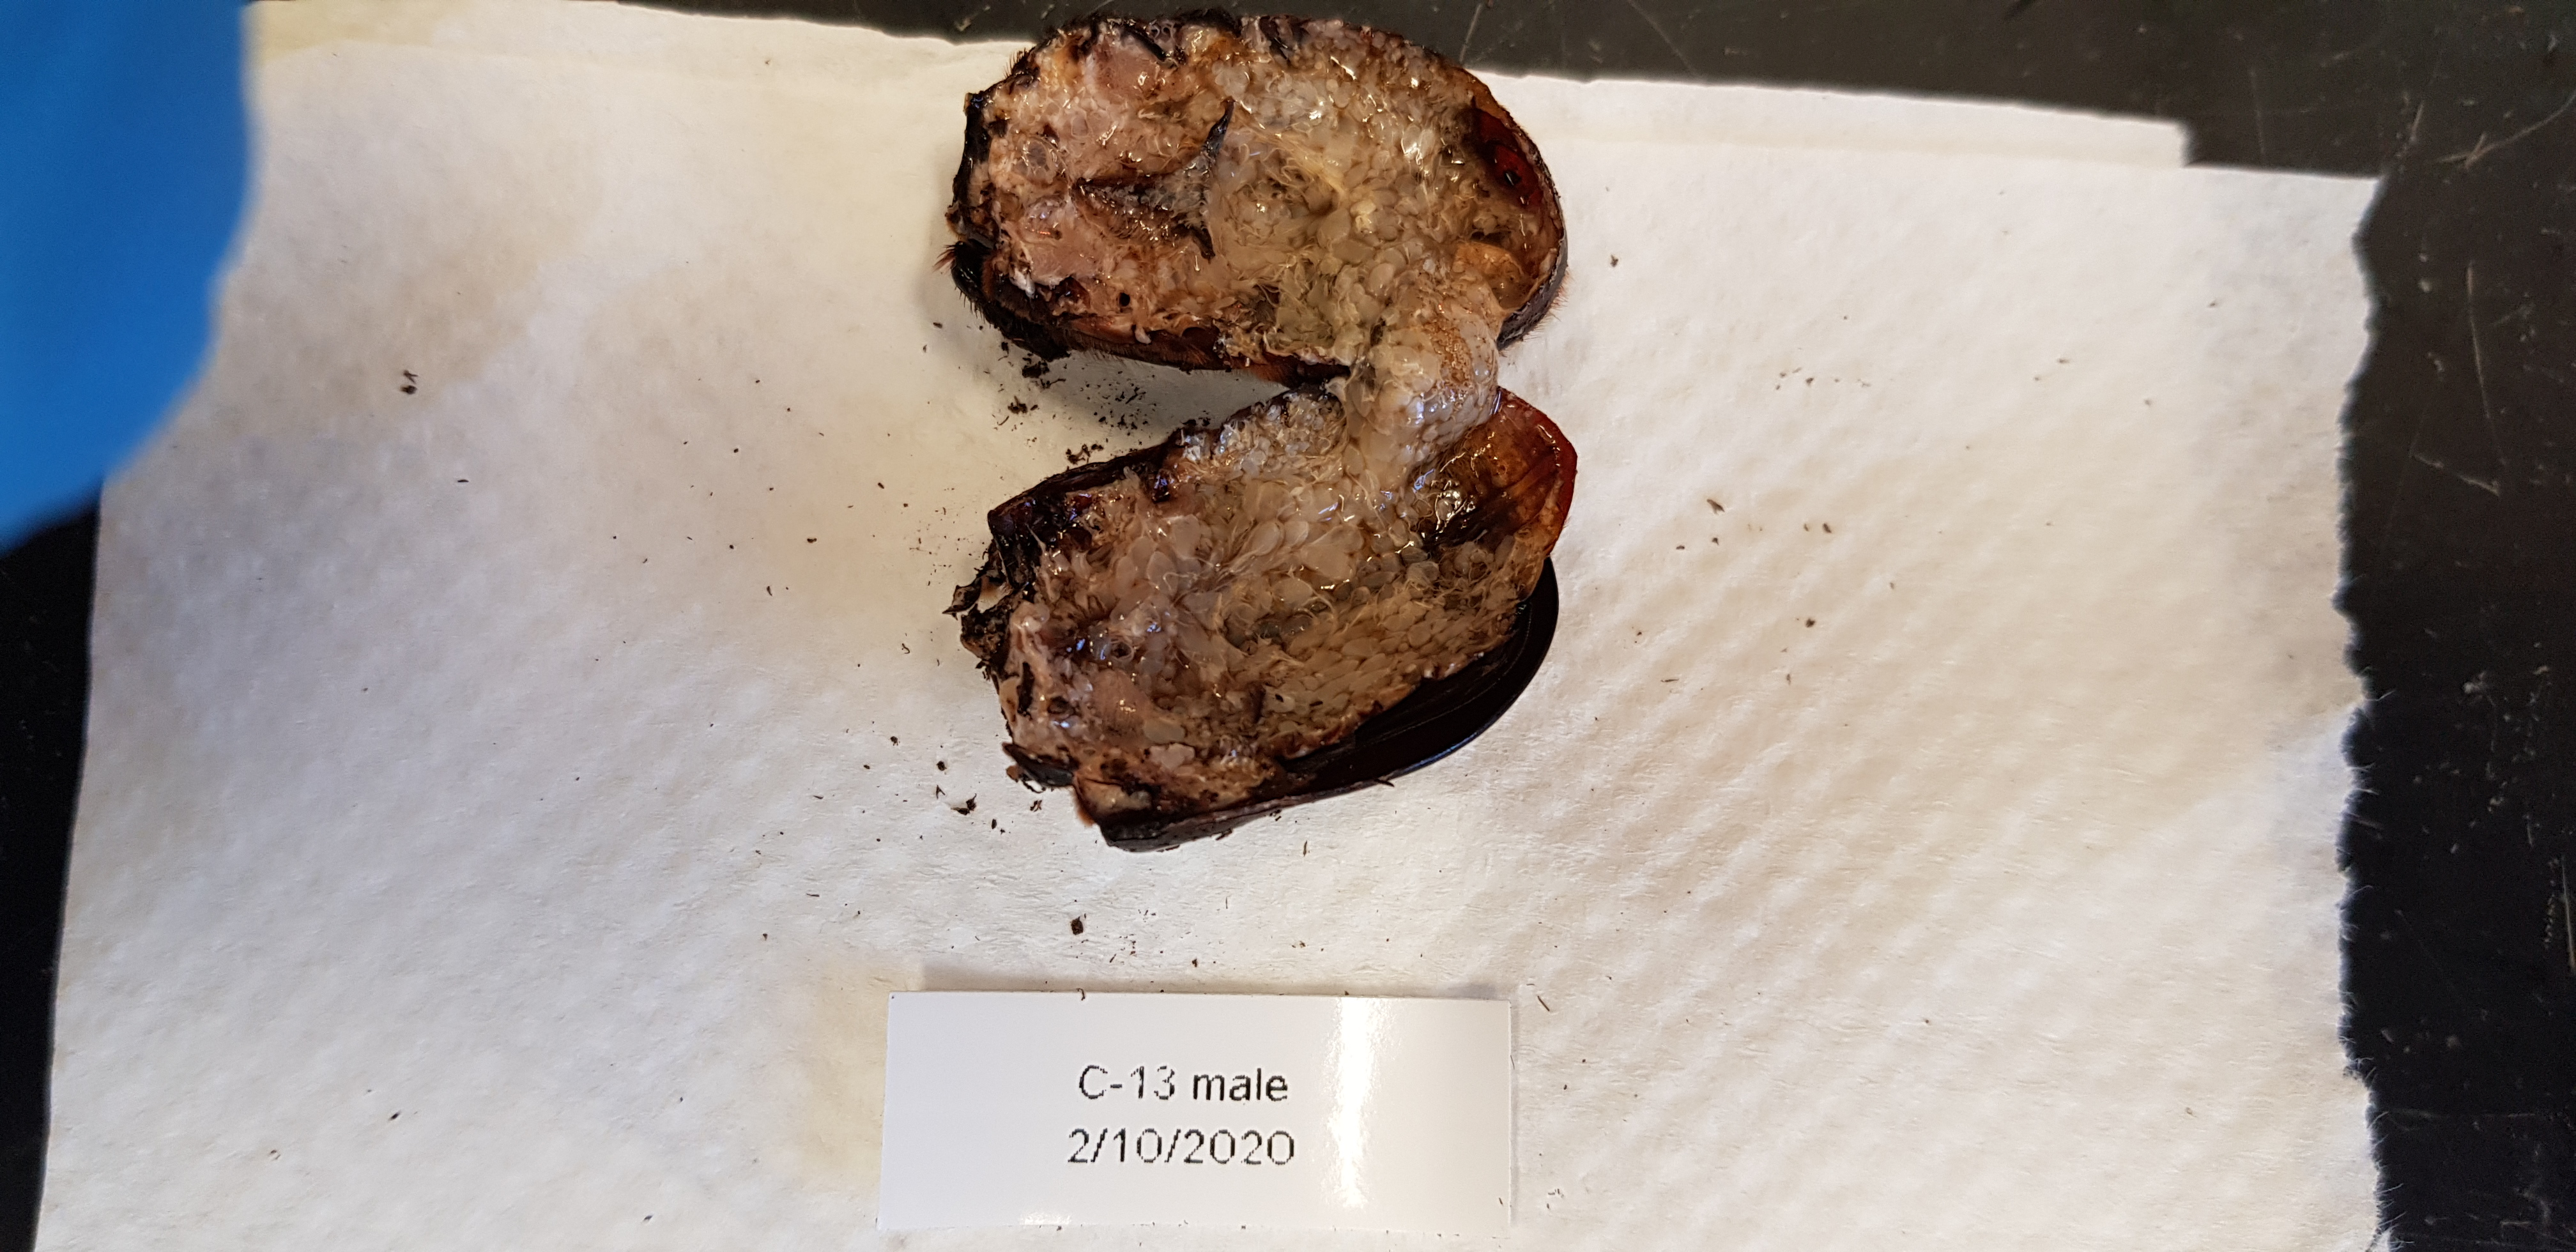
\includegraphics[width=\textwidth]{pm-images/20200210_151921.jpg}
\caption{\textbf{C13m} jar\_id                                 C13
sex                                      m
treatment                             none
date\_treated           2019-12-27 00:00:00
date\_died                              NaT
postmortem\_virus                       NaN
postmortem\_bacteria                    NaN
pm\_image\_filename      20200210\_151921.jpg
date\_end\_bioassay      2020-02-06 00:00:00
t                                       41
e                                    False
Name: 12, dtype: object}
\end{figure}
\clearpage

\begin{figure}[h!]
\centering
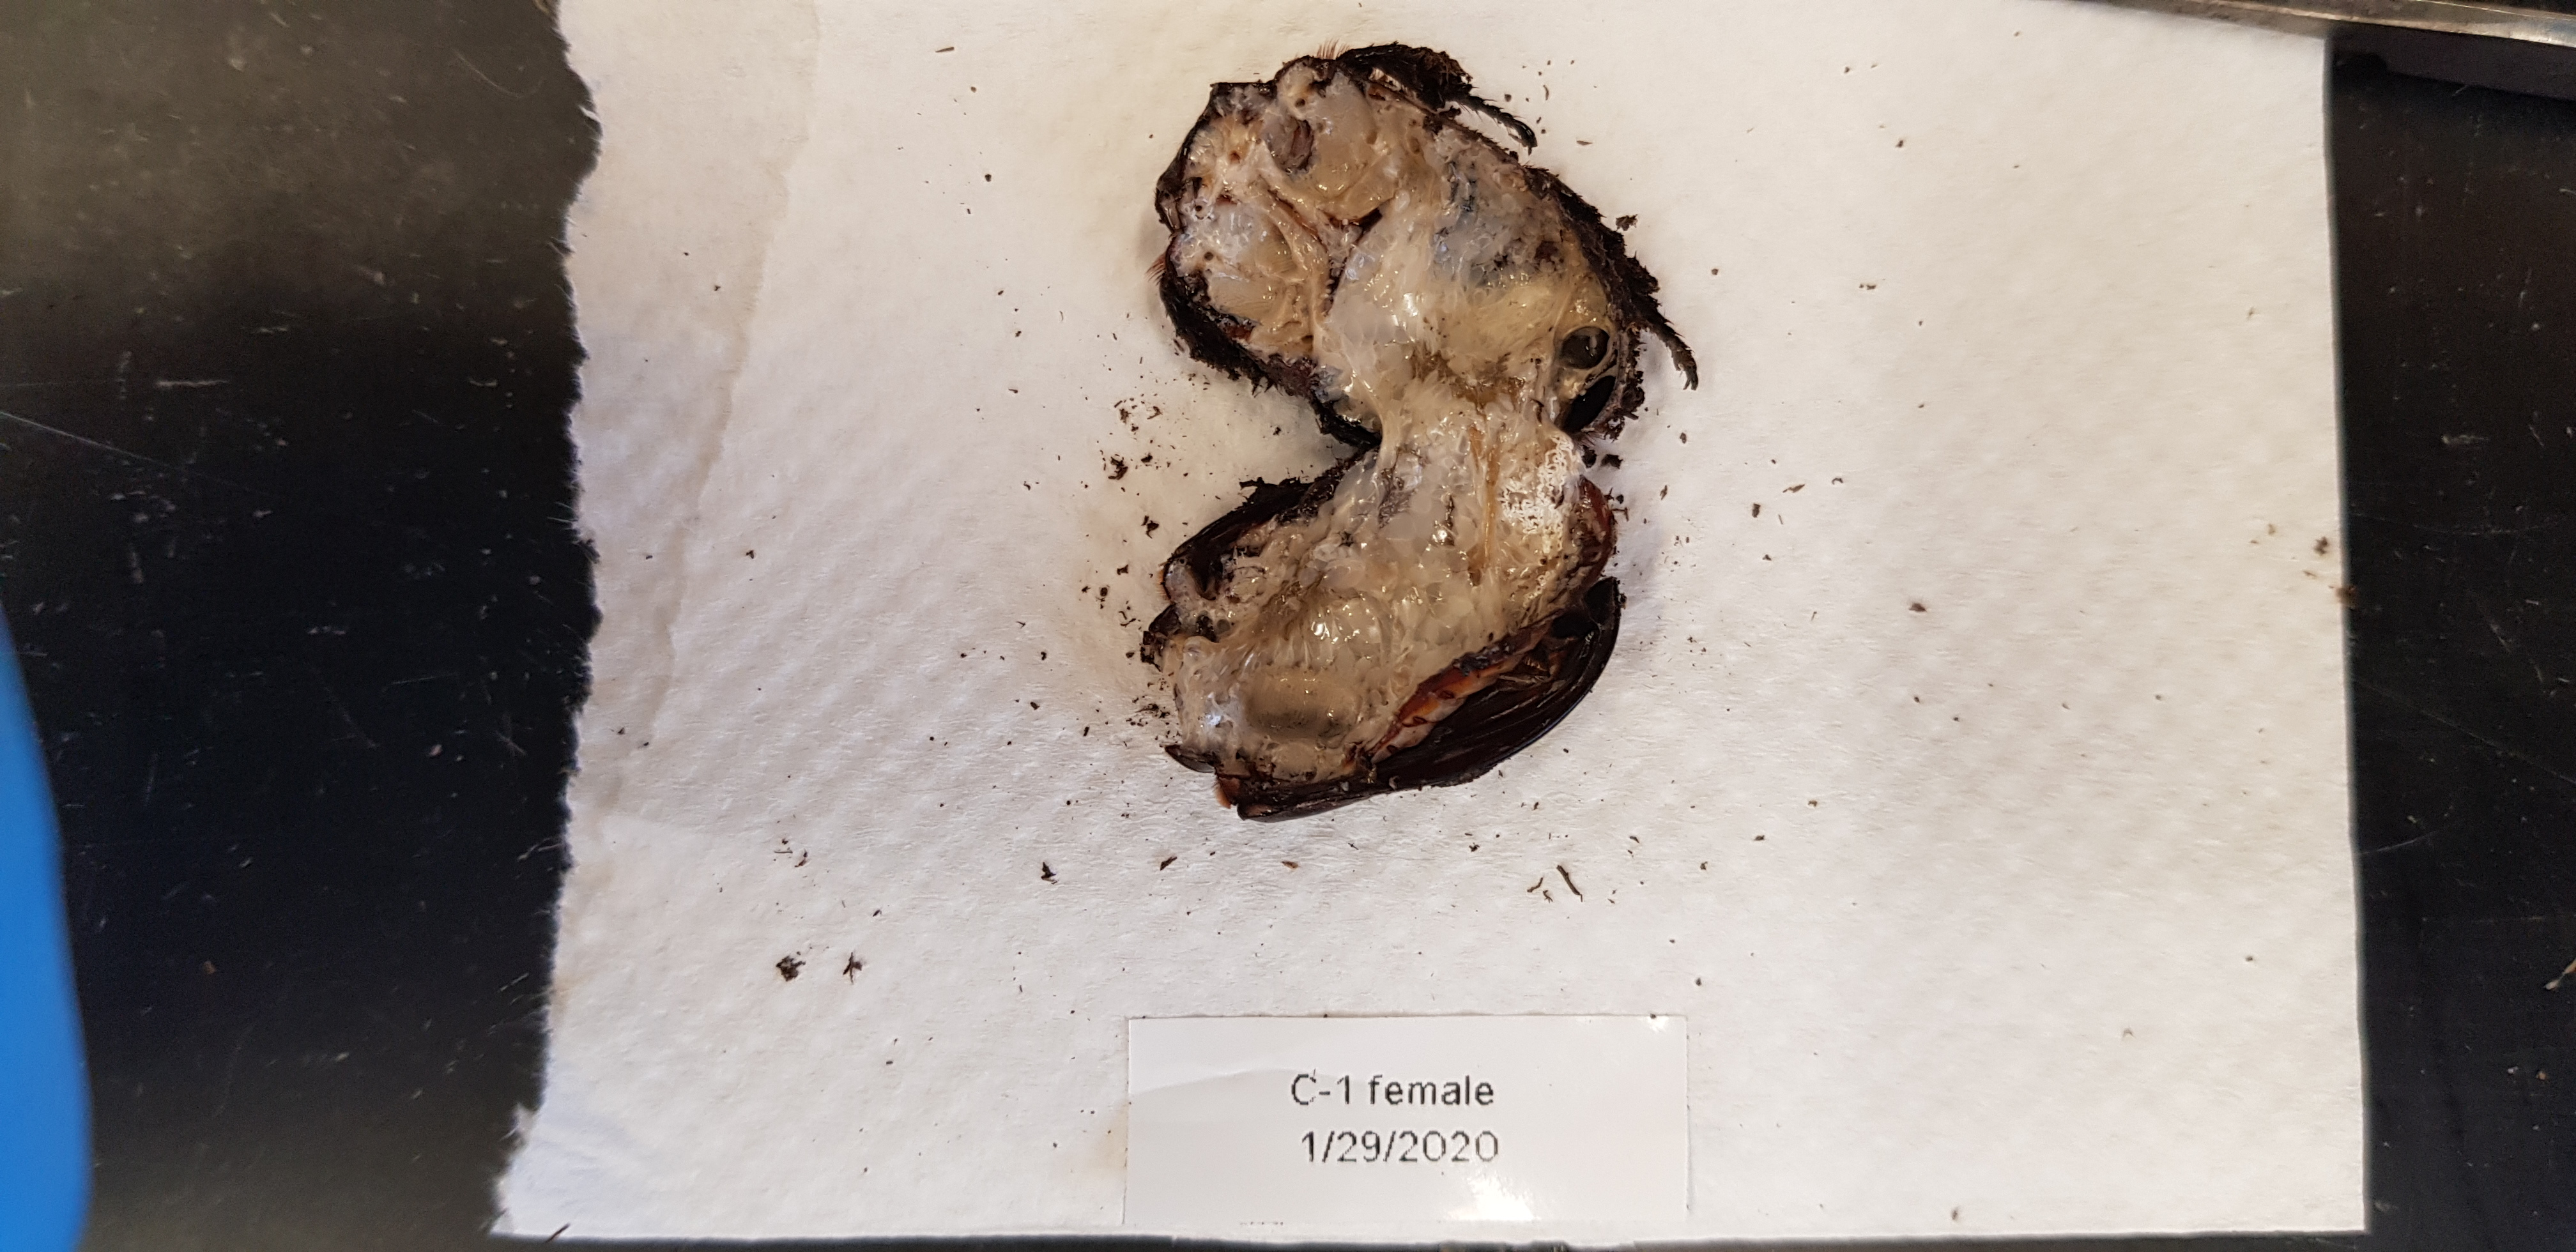
\includegraphics[width=\textwidth]{pm-images/20200129_151721.jpg}
\caption{\textbf{C1f} jar\_id                                  C1
sex                                      f
treatment                             none
date\_treated           2019-12-26 00:00:00
date\_died              2020-01-29 00:00:00
postmortem\_virus                       NaN
postmortem\_bacteria                    NaN
pm\_image\_filename      20200129\_151721.jpg
date\_end\_bioassay      2020-02-06 00:00:00
t                                       34
e                                     True
Name: 15, dtype: object}
\end{figure}
\clearpage

\begin{figure}[h!]
\centering
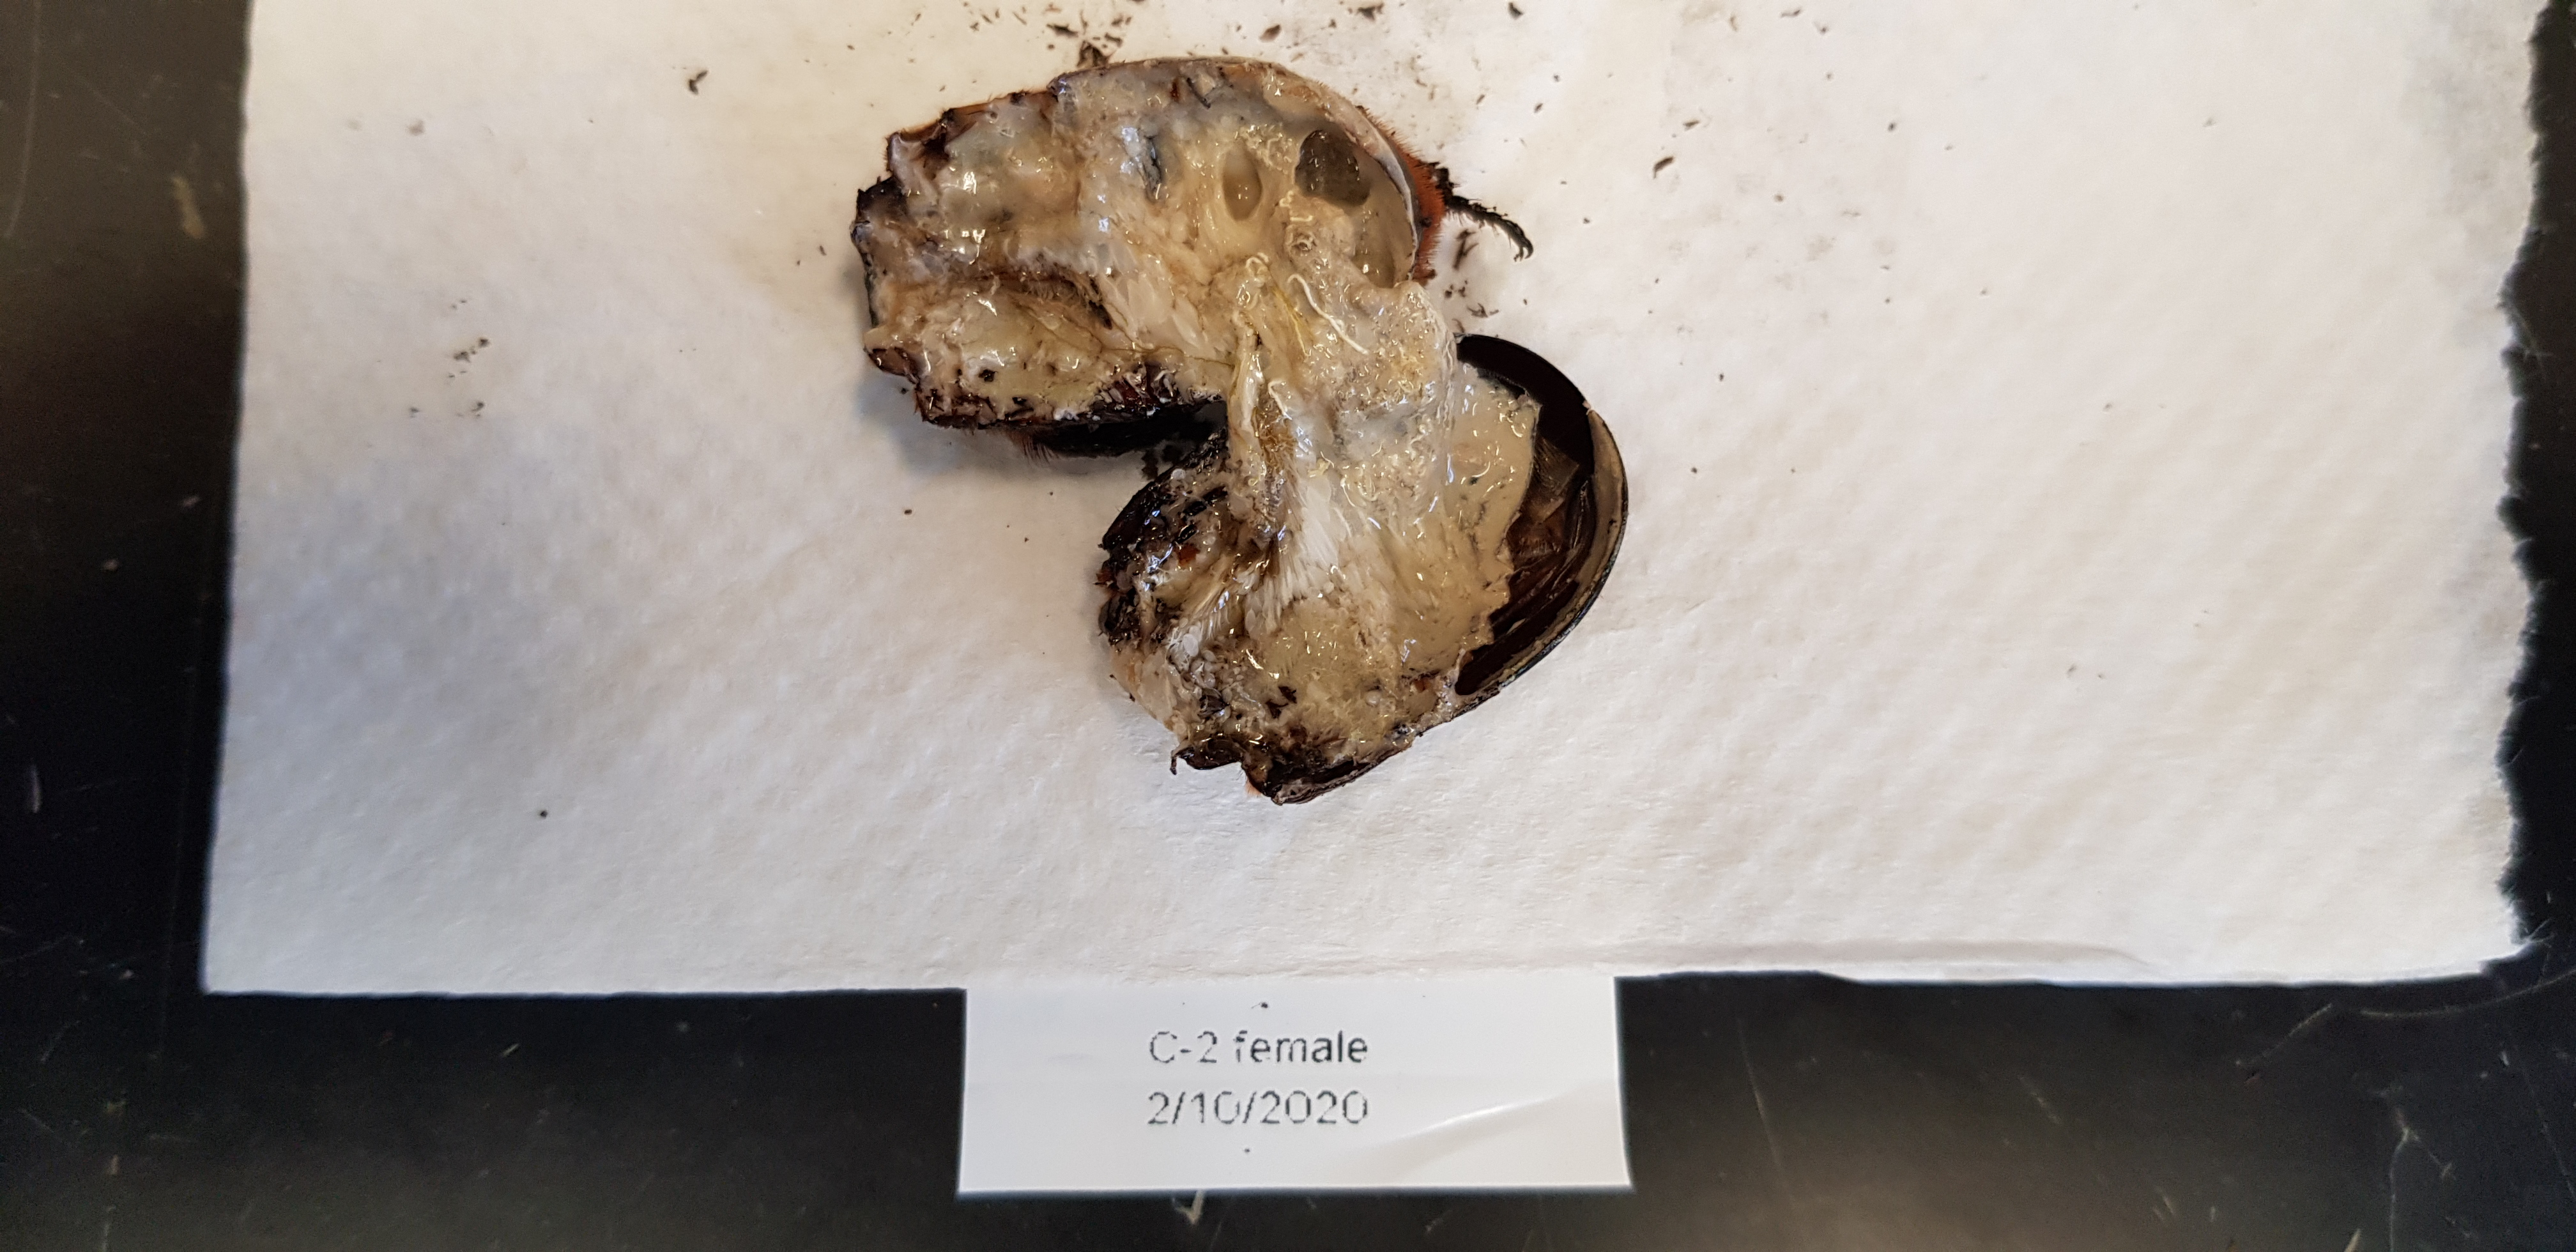
\includegraphics[width=\textwidth]{pm-images/20200210_145205.jpg}
\caption{\textbf{C2f} jar\_id                                  C2
sex                                      f
treatment                             none
date\_treated           2019-12-26 00:00:00
date\_died                              NaT
postmortem\_virus                       NaN
postmortem\_bacteria                    NaN
pm\_image\_filename      20200210\_145205.jpg
date\_end\_bioassay      2020-02-06 00:00:00
t                                       42
e                                    False
Name: 16, dtype: object}
\end{figure}
\clearpage

\begin{figure}[h!]
\centering
\includegraphics[width=\textwidth]{pm-images/20200129_161111.jpg}
\caption{\textbf{C3f} jar\_id                                  C3
sex                                      f
treatment                             none
date\_treated           2019-12-26 00:00:00
date\_died              2020-01-29 00:00:00
postmortem\_virus                       NaN
postmortem\_bacteria                    NaN
pm\_image\_filename      20200129\_161111.jpg
date\_end\_bioassay      2020-02-06 00:00:00
t                                       34
e                                     True
Name: 17, dtype: object}
\end{figure}
\clearpage

\begin{figure}[h!]
\centering
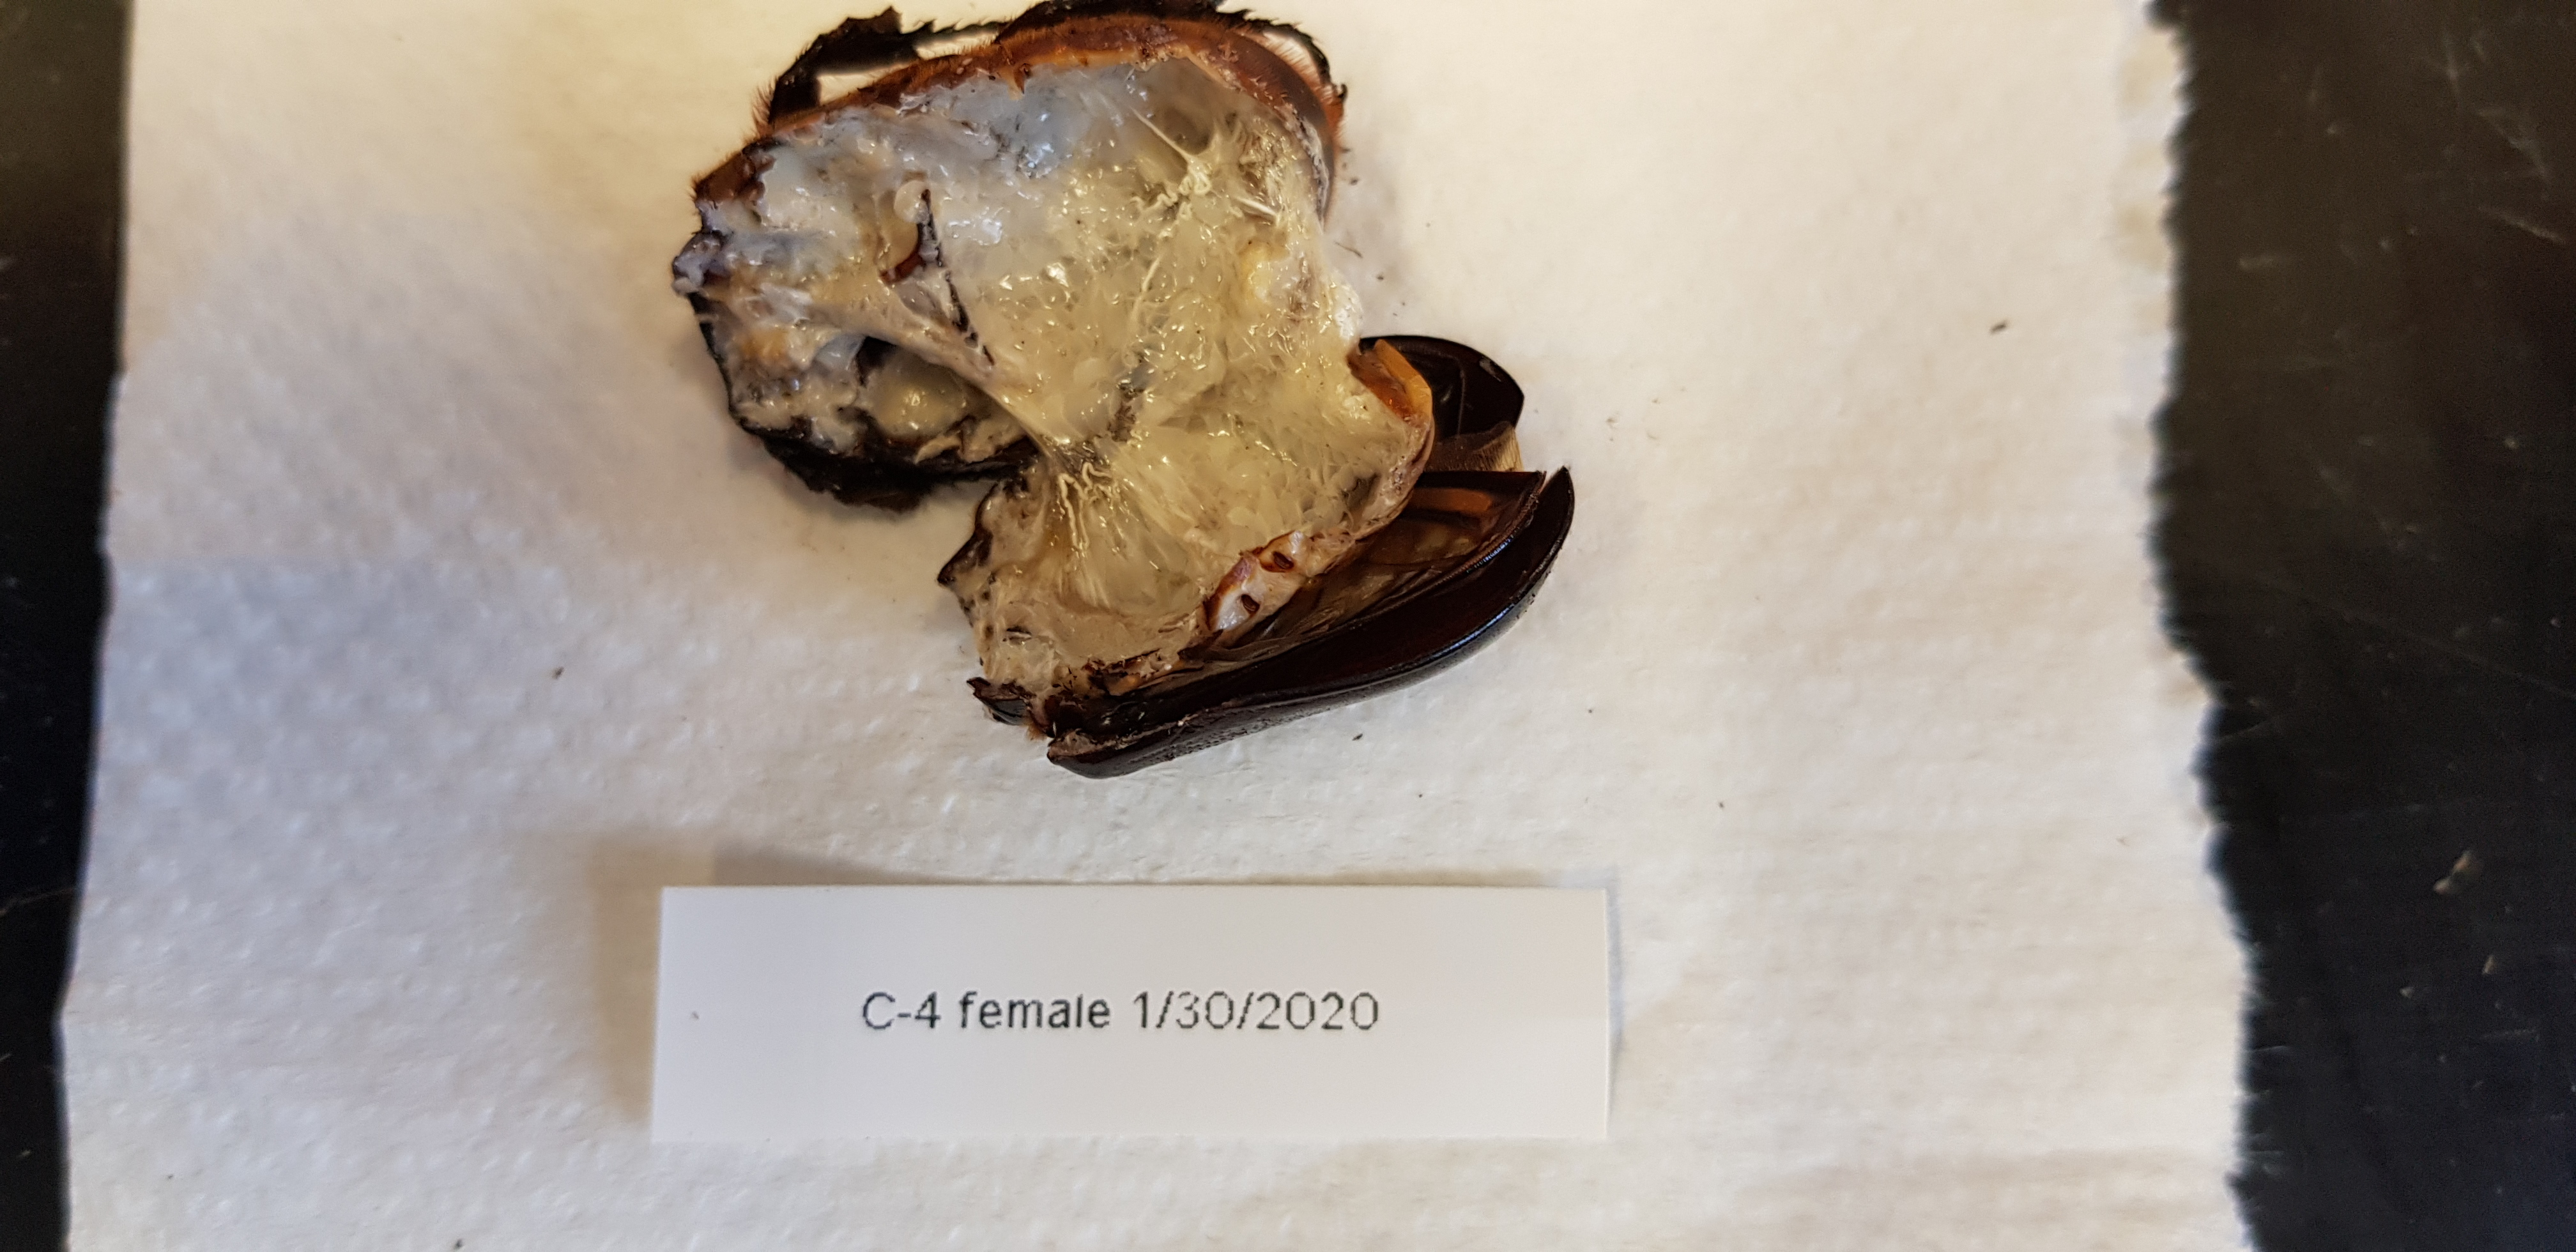
\includegraphics[width=\textwidth]{pm-images/20200131_113359.jpg}
\caption{\textbf{C4f} jar\_id                                  C4
sex                                      f
treatment                             none
date\_treated           2019-12-26 00:00:00
date\_died              2020-01-31 00:00:00
postmortem\_virus                       NaN
postmortem\_bacteria                    NaN
pm\_image\_filename      20200131\_113359.jpg
date\_end\_bioassay      2020-02-06 00:00:00
t                                       36
e                                     True
Name: 18, dtype: object}
\end{figure}
\clearpage

\begin{figure}[h!]
\centering
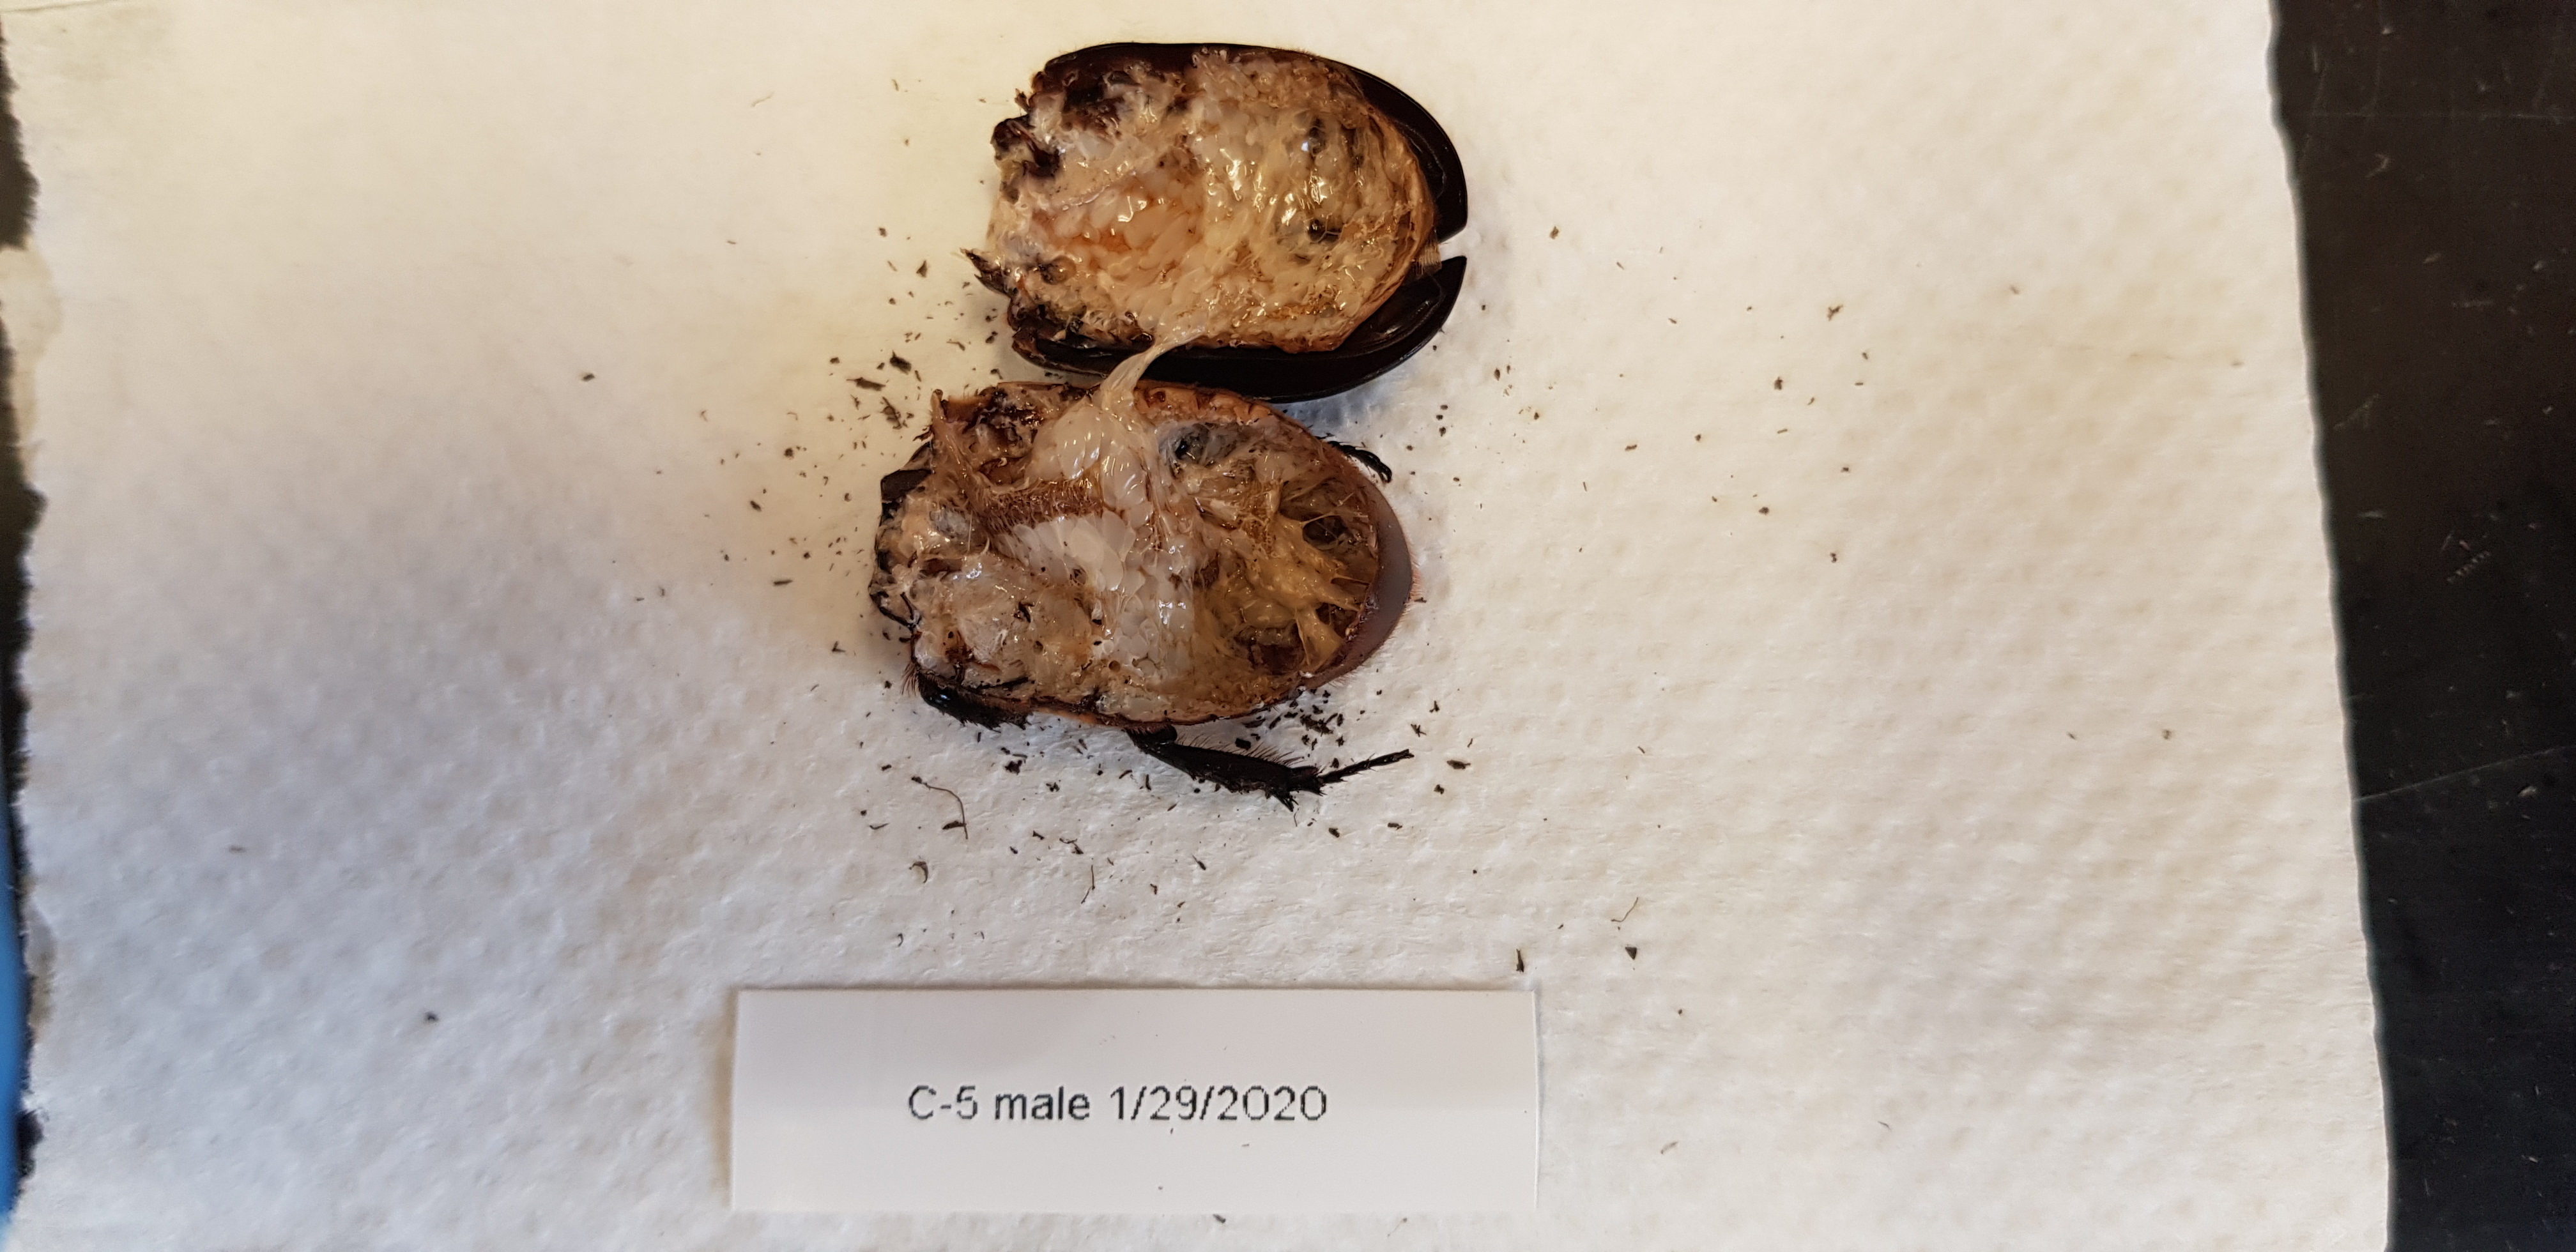
\includegraphics[width=\textwidth]{pm-images/20200129_143353.jpg}
\caption{\textbf{C5f} jar\_id                                  C5
sex                                      f
treatment                             none
date\_treated           2019-12-26 00:00:00
date\_died                              NaT
postmortem\_virus                       NaN
postmortem\_bacteria                    NaN
pm\_image\_filename      20200129\_143353.jpg
date\_end\_bioassay      2020-02-06 00:00:00
t                                       42
e                                    False
Name: 19, dtype: object}
\end{figure}
\clearpage

\begin{figure}[h!]
\centering
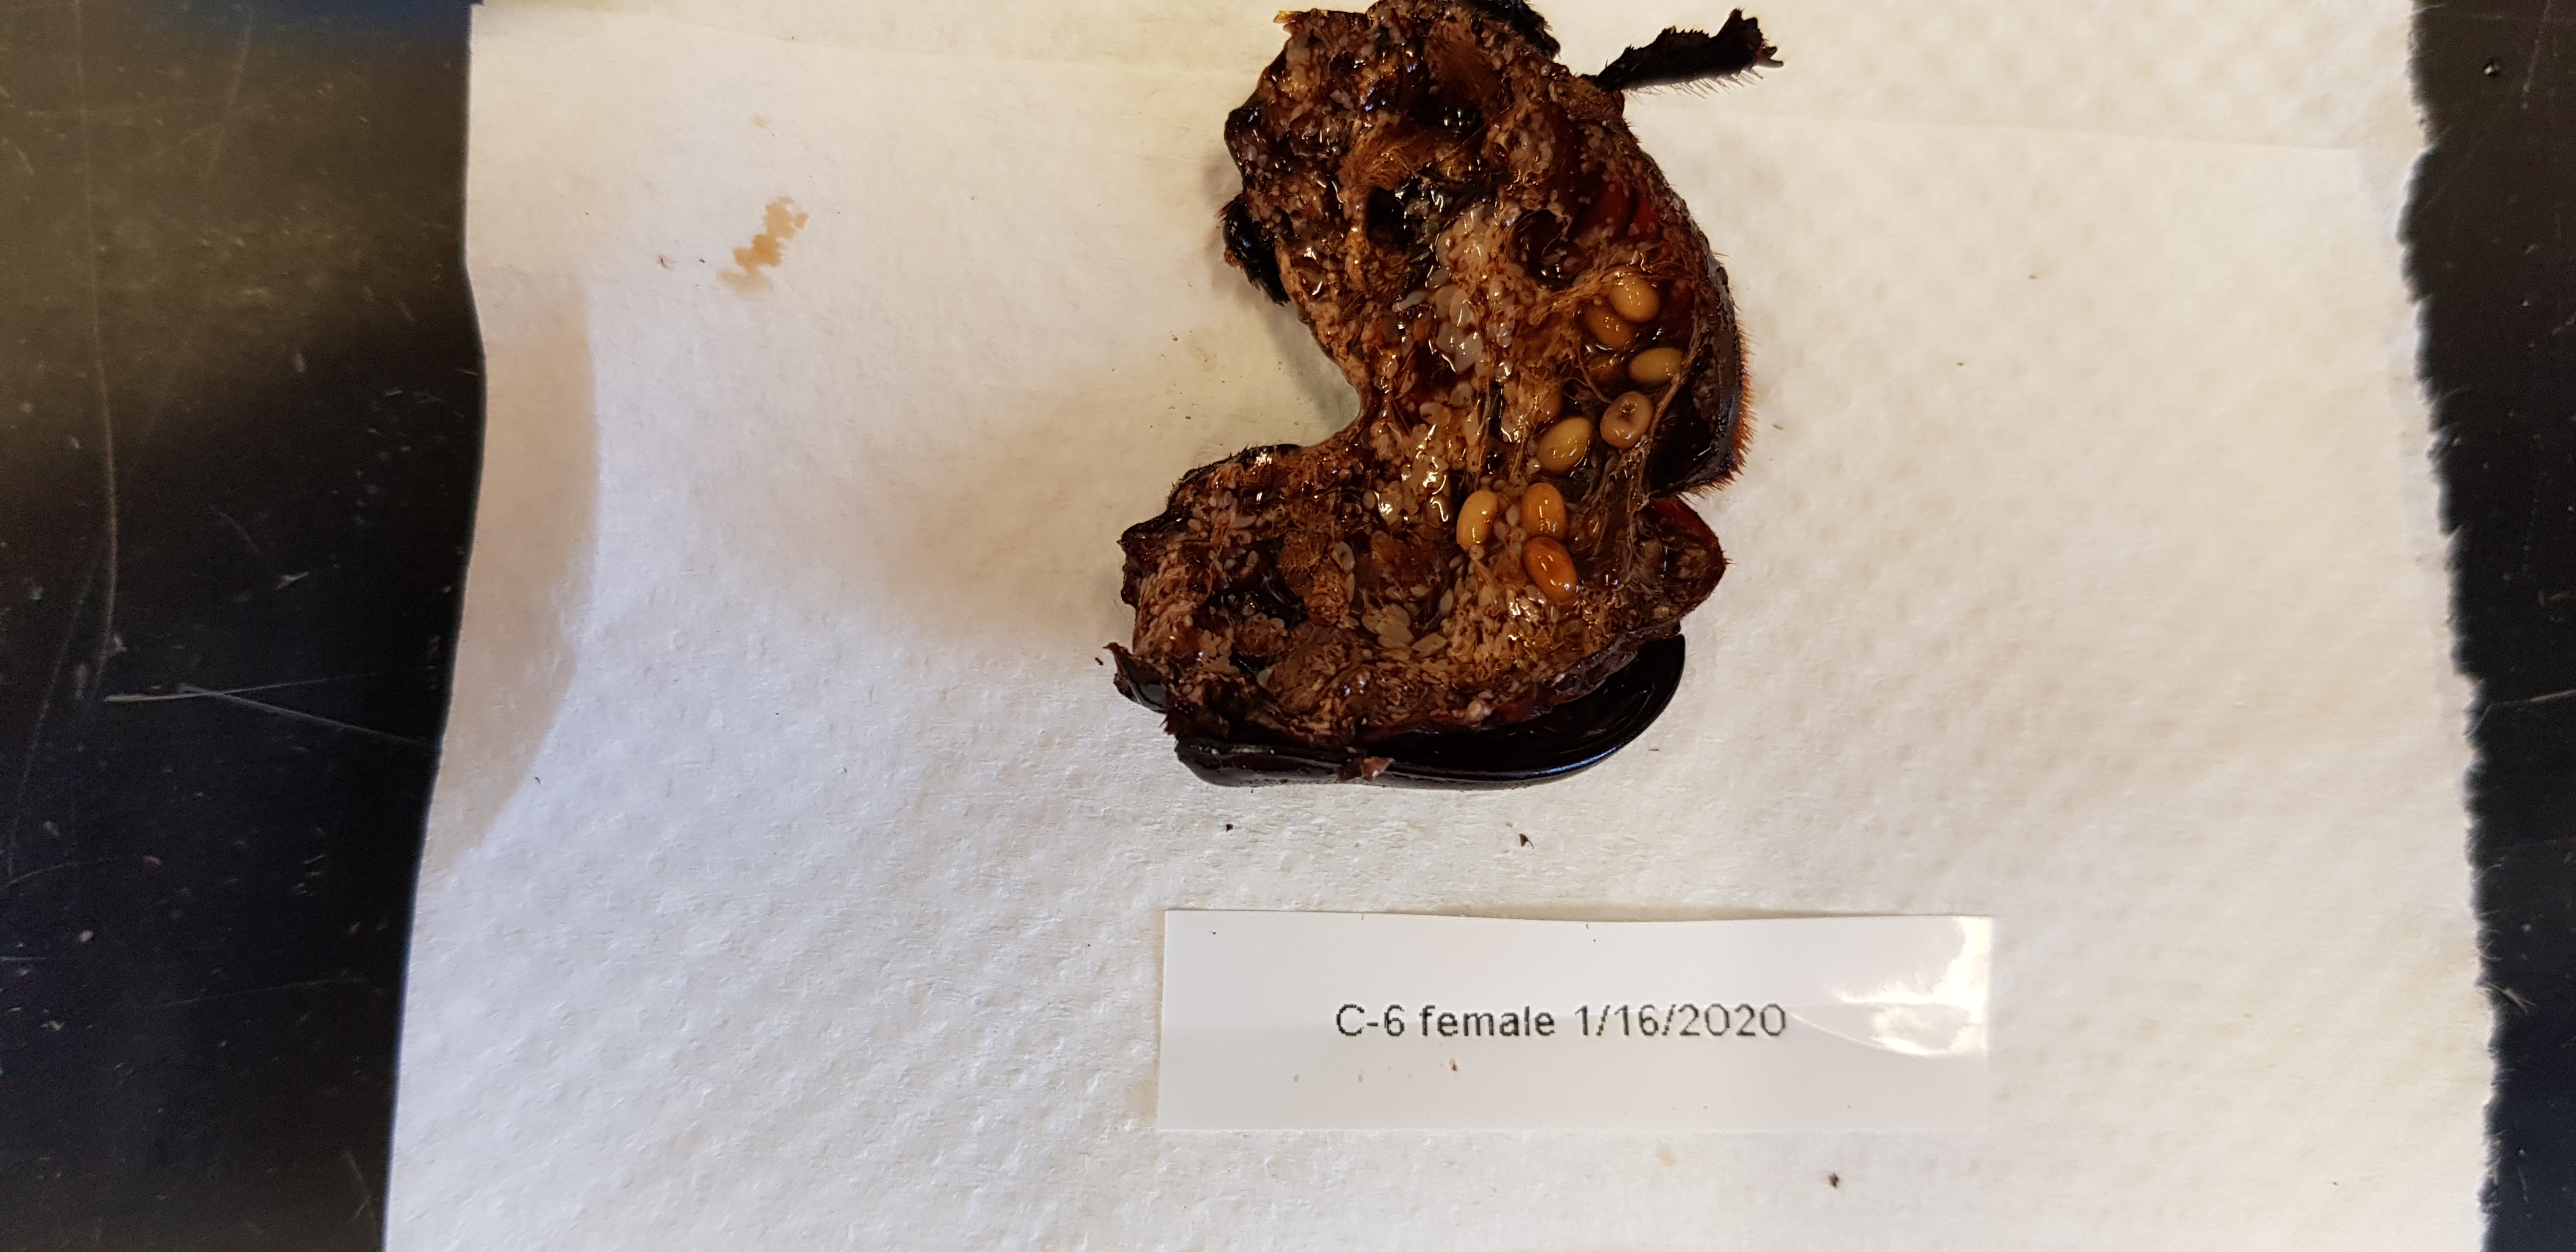
\includegraphics[width=\textwidth]{pm-images/20200116_110642.jpg}
\caption{\textbf{C6f} jar\_id                                  C6
sex                                      f
treatment                             none
date\_treated           2019-12-27 00:00:00
date\_died              2020-01-16 00:00:00
postmortem\_virus                       NaN
postmortem\_bacteria                      1
pm\_image\_filename      20200116\_110642.jpg
date\_end\_bioassay      2020-02-06 00:00:00
t                                       20
e                                     True
Name: 20, dtype: object}
\end{figure}
\clearpage

\begin{figure}[h!]
\centering
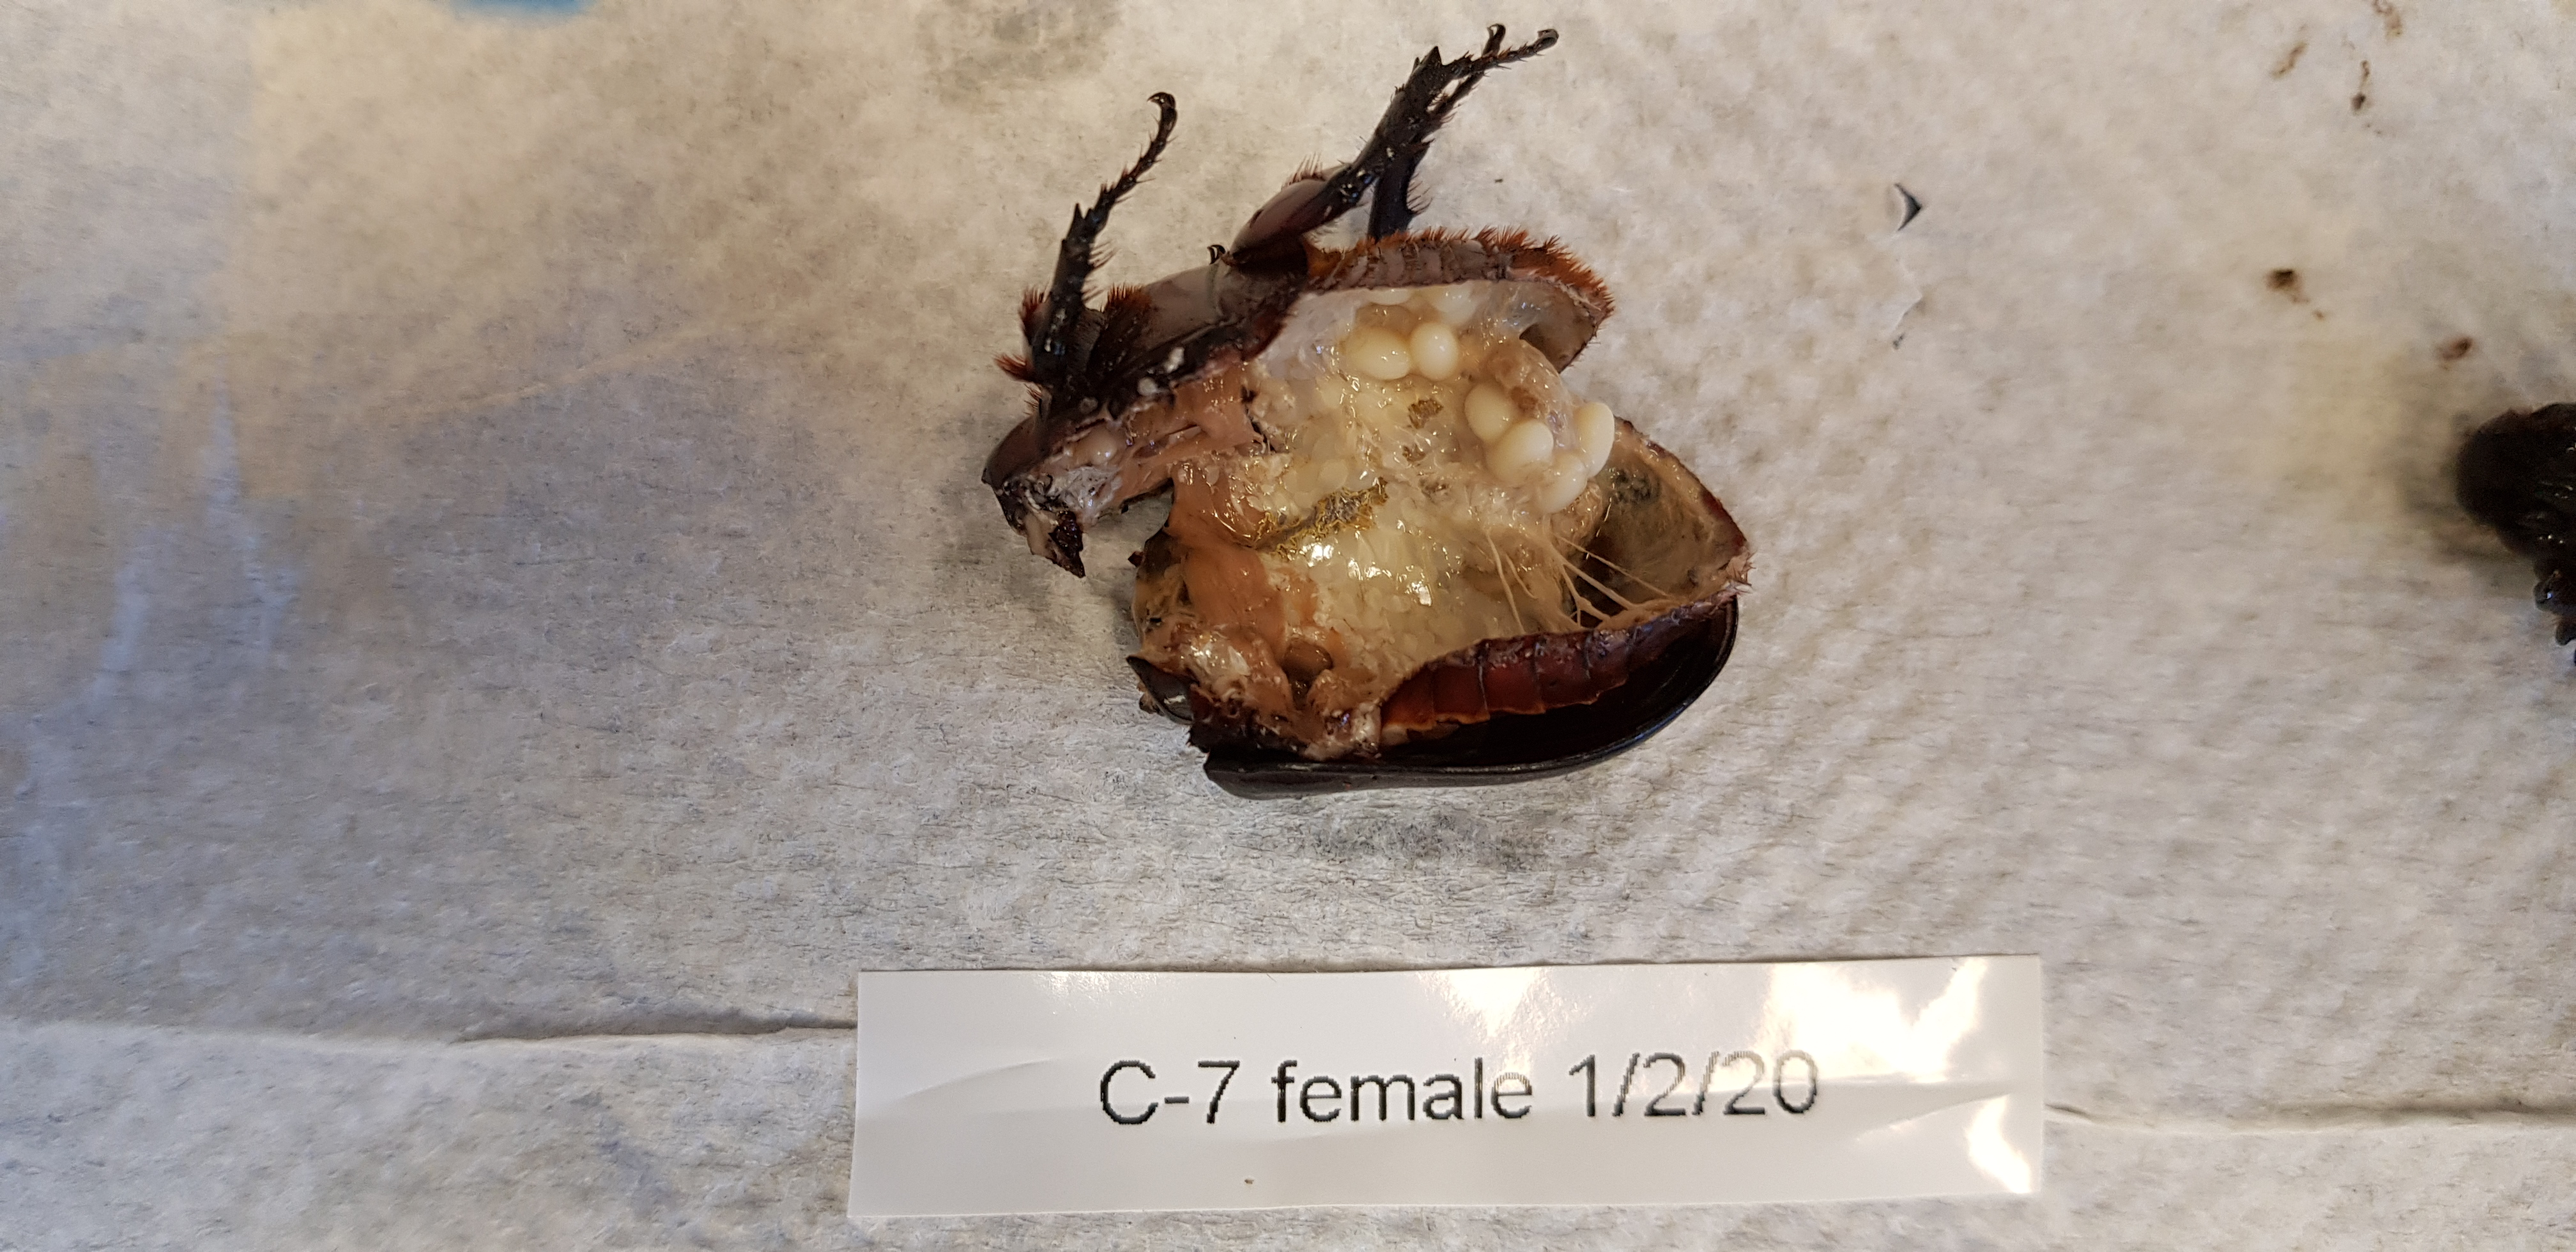
\includegraphics[width=\textwidth]{pm-images/20200102_112130.jpg}
\caption{\textbf{C7f} jar\_id                                  C7
sex                                      f
treatment                             none
date\_treated           2019-12-27 00:00:00
date\_died              2020-01-02 00:00:00
postmortem\_virus                       NaN
postmortem\_bacteria                    NaN
pm\_image\_filename      20200102\_112130.jpg
date\_end\_bioassay      2020-02-06 00:00:00
t                                        6
e                                     True
Name: 21, dtype: object}
\end{figure}
\clearpage

\begin{figure}[h!]
\centering
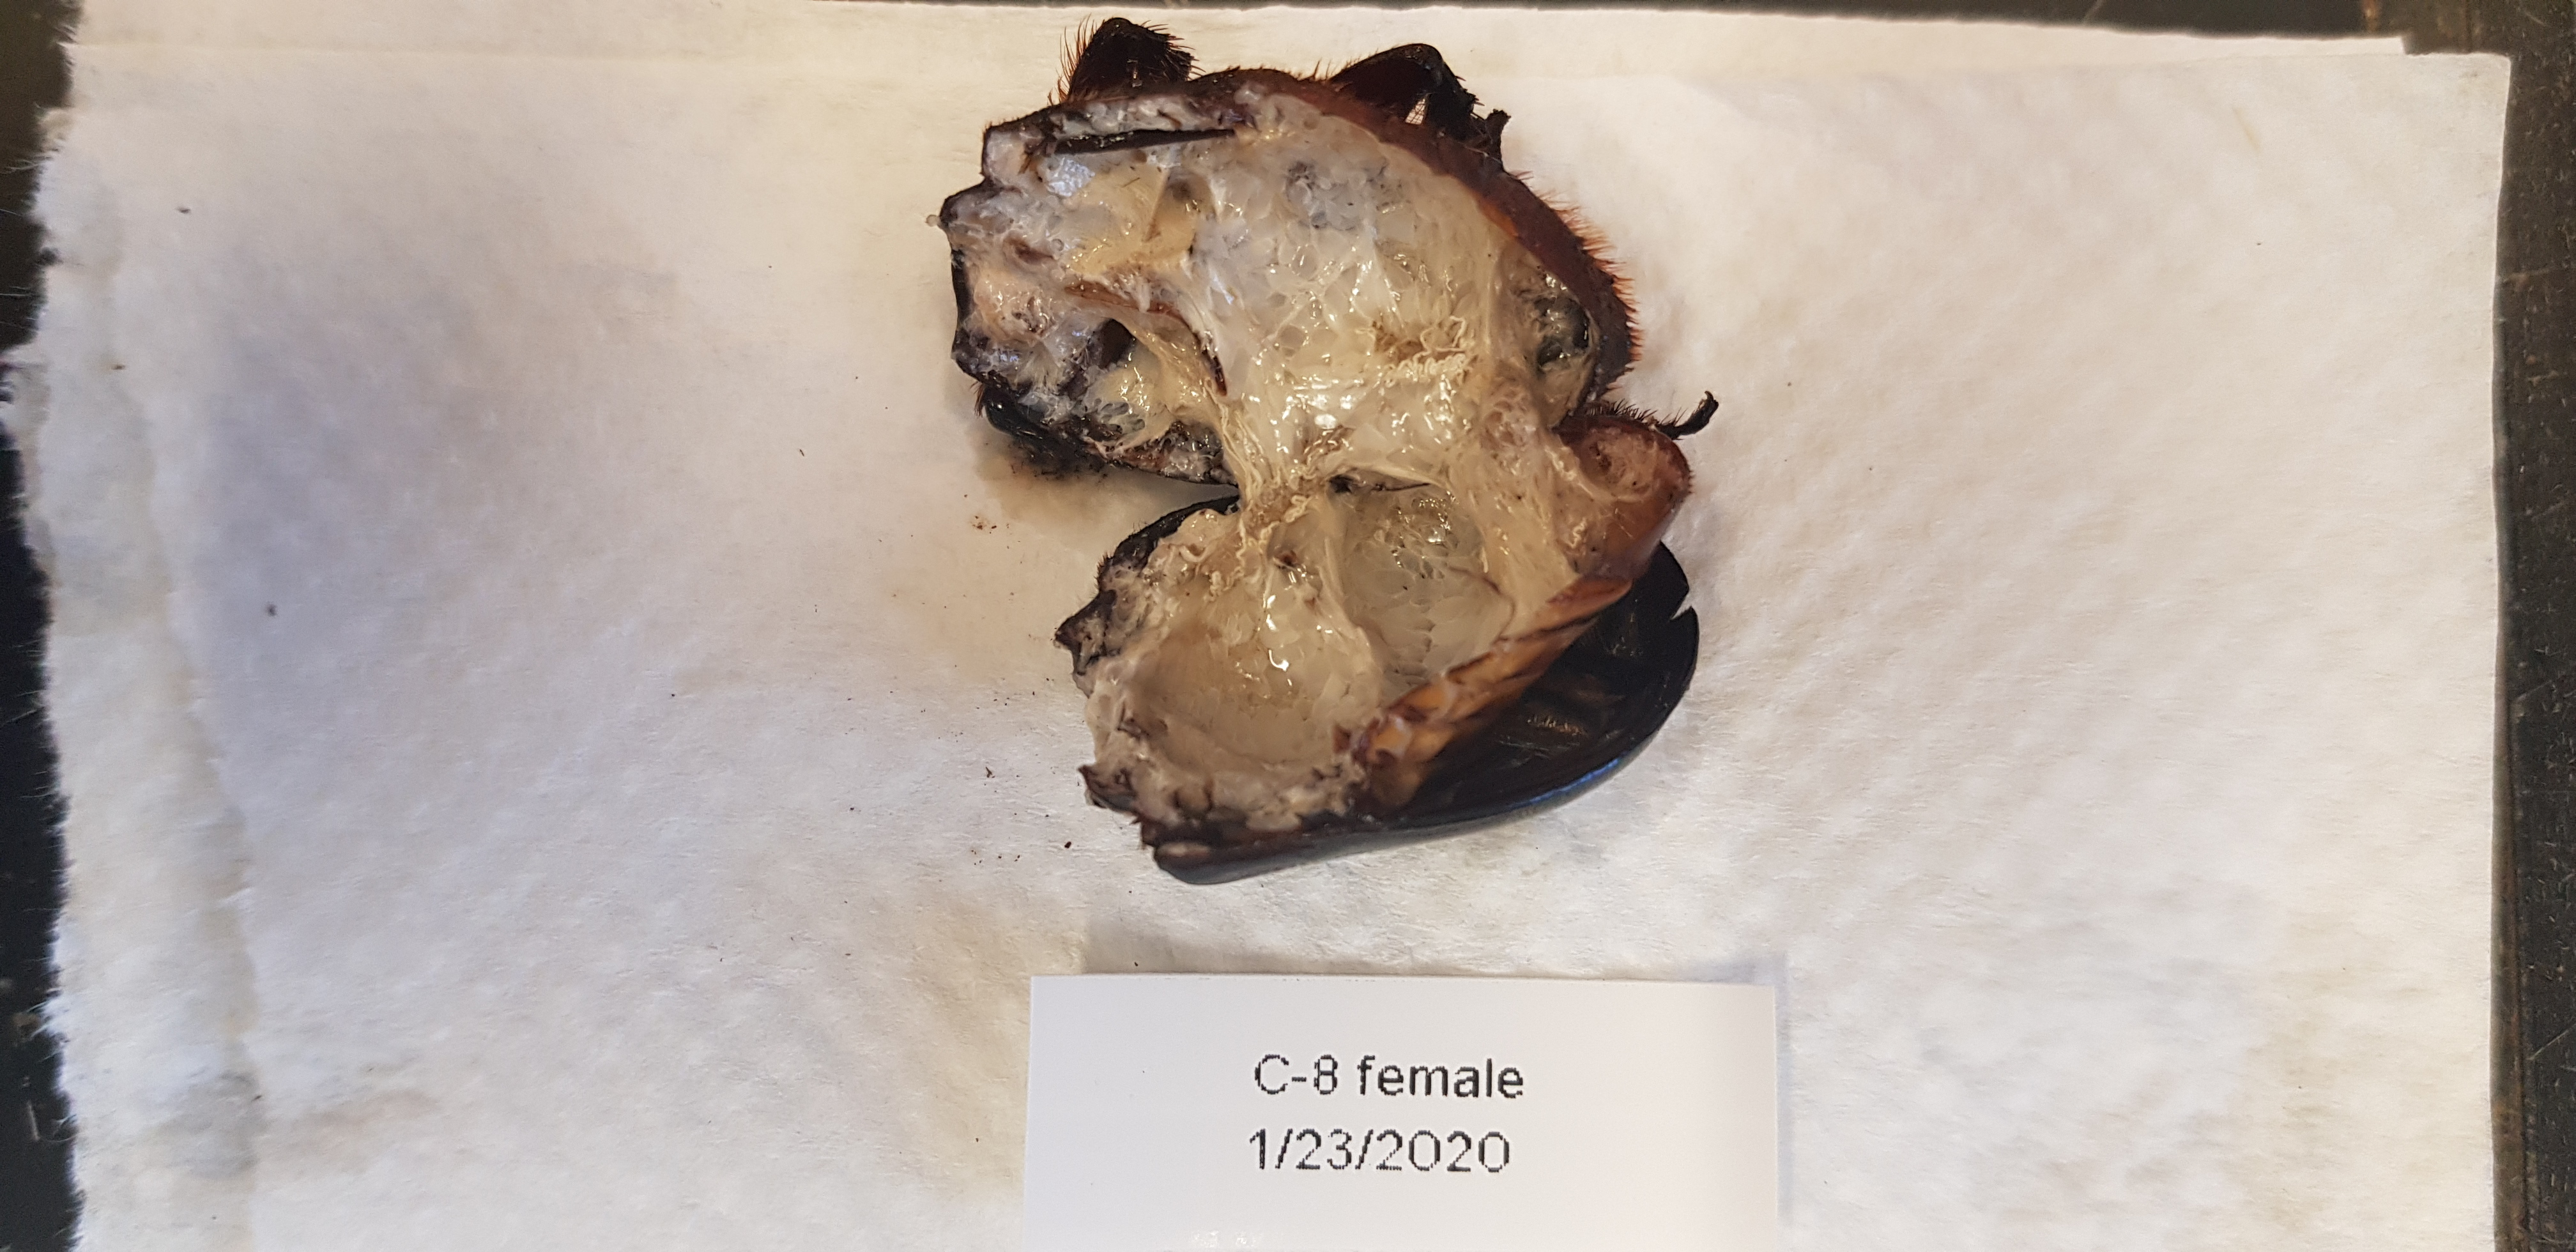
\includegraphics[width=\textwidth]{pm-images/20200123_163225.jpg}
\caption{\textbf{C8f} jar\_id                                  C8
sex                                      f
treatment                             none
date\_treated           2019-12-27 00:00:00
date\_died              2020-01-23 00:00:00
postmortem\_virus                       NaN
postmortem\_bacteria                    NaN
pm\_image\_filename      20200123\_163225.jpg
date\_end\_bioassay      2020-02-06 00:00:00
t                                       27
e                                     True
Name: 22, dtype: object}
\end{figure}
\clearpage

\begin{figure}[h!]
\centering
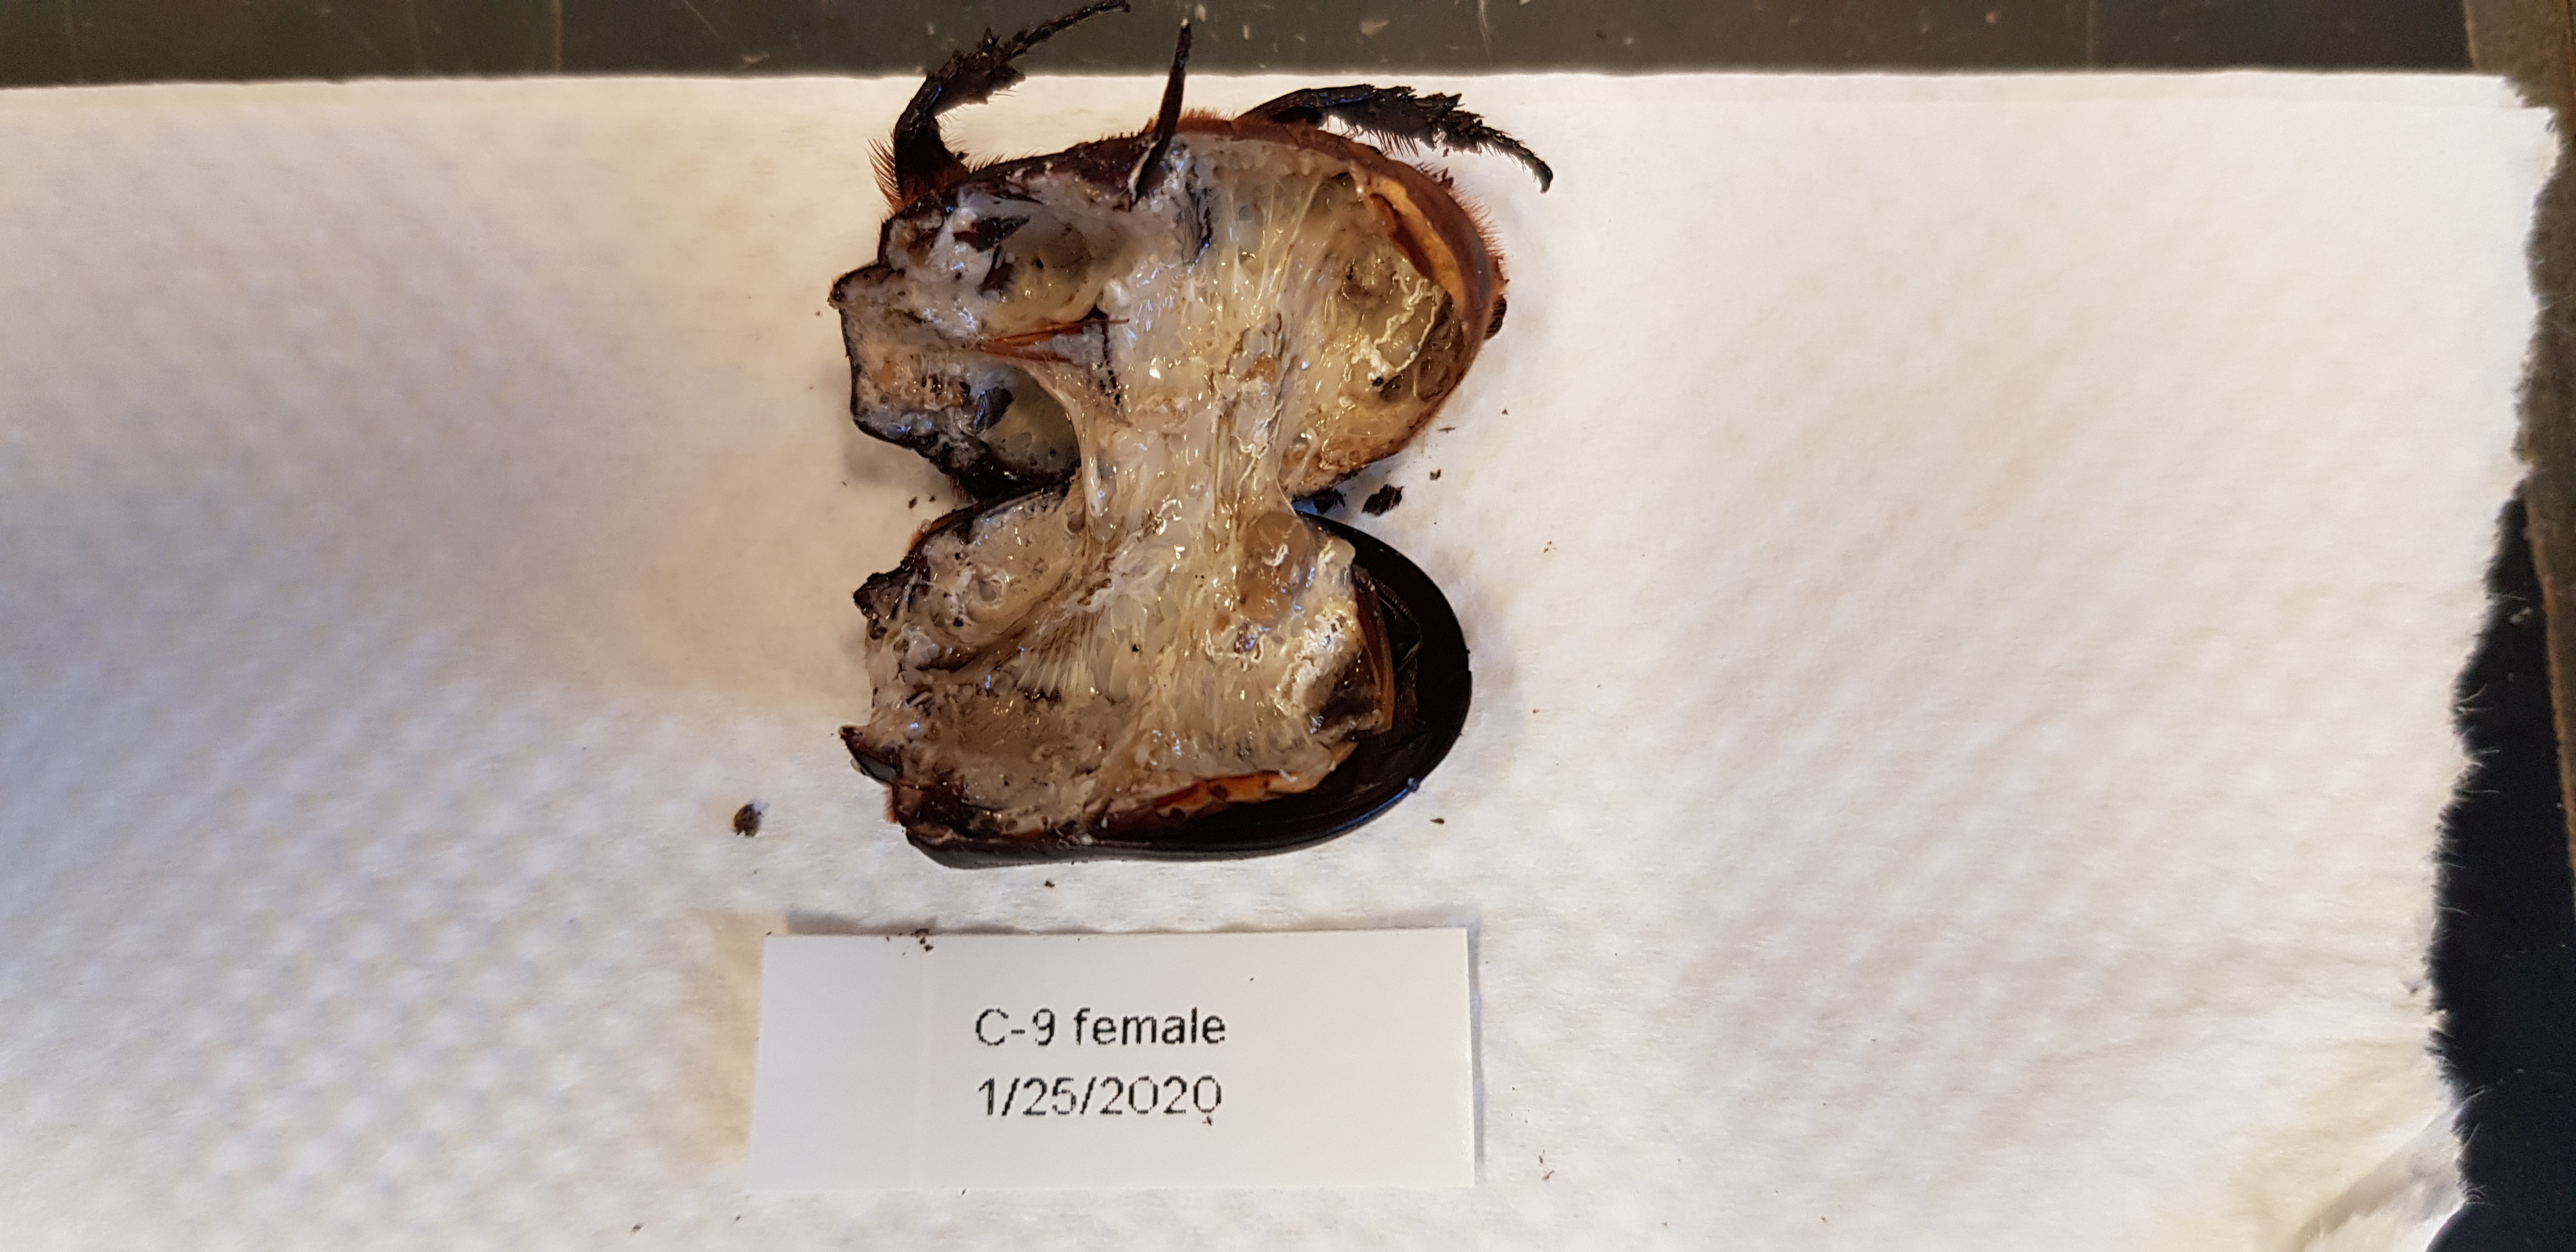
\includegraphics[width=\textwidth]{pm-images/20200125_121834.jpg}
\caption{\textbf{C9f} jar\_id                                  C9
sex                                      f
treatment                             none
date\_treated           2019-12-27 00:00:00
date\_died                              NaT
postmortem\_virus                       NaN
postmortem\_bacteria                    NaN
pm\_image\_filename      20200125\_121834.jpg
date\_end\_bioassay      2020-02-06 00:00:00
t                                       41
e                                    False
Name: 23, dtype: object}
\end{figure}
\clearpage

\begin{figure}[h!]
\centering
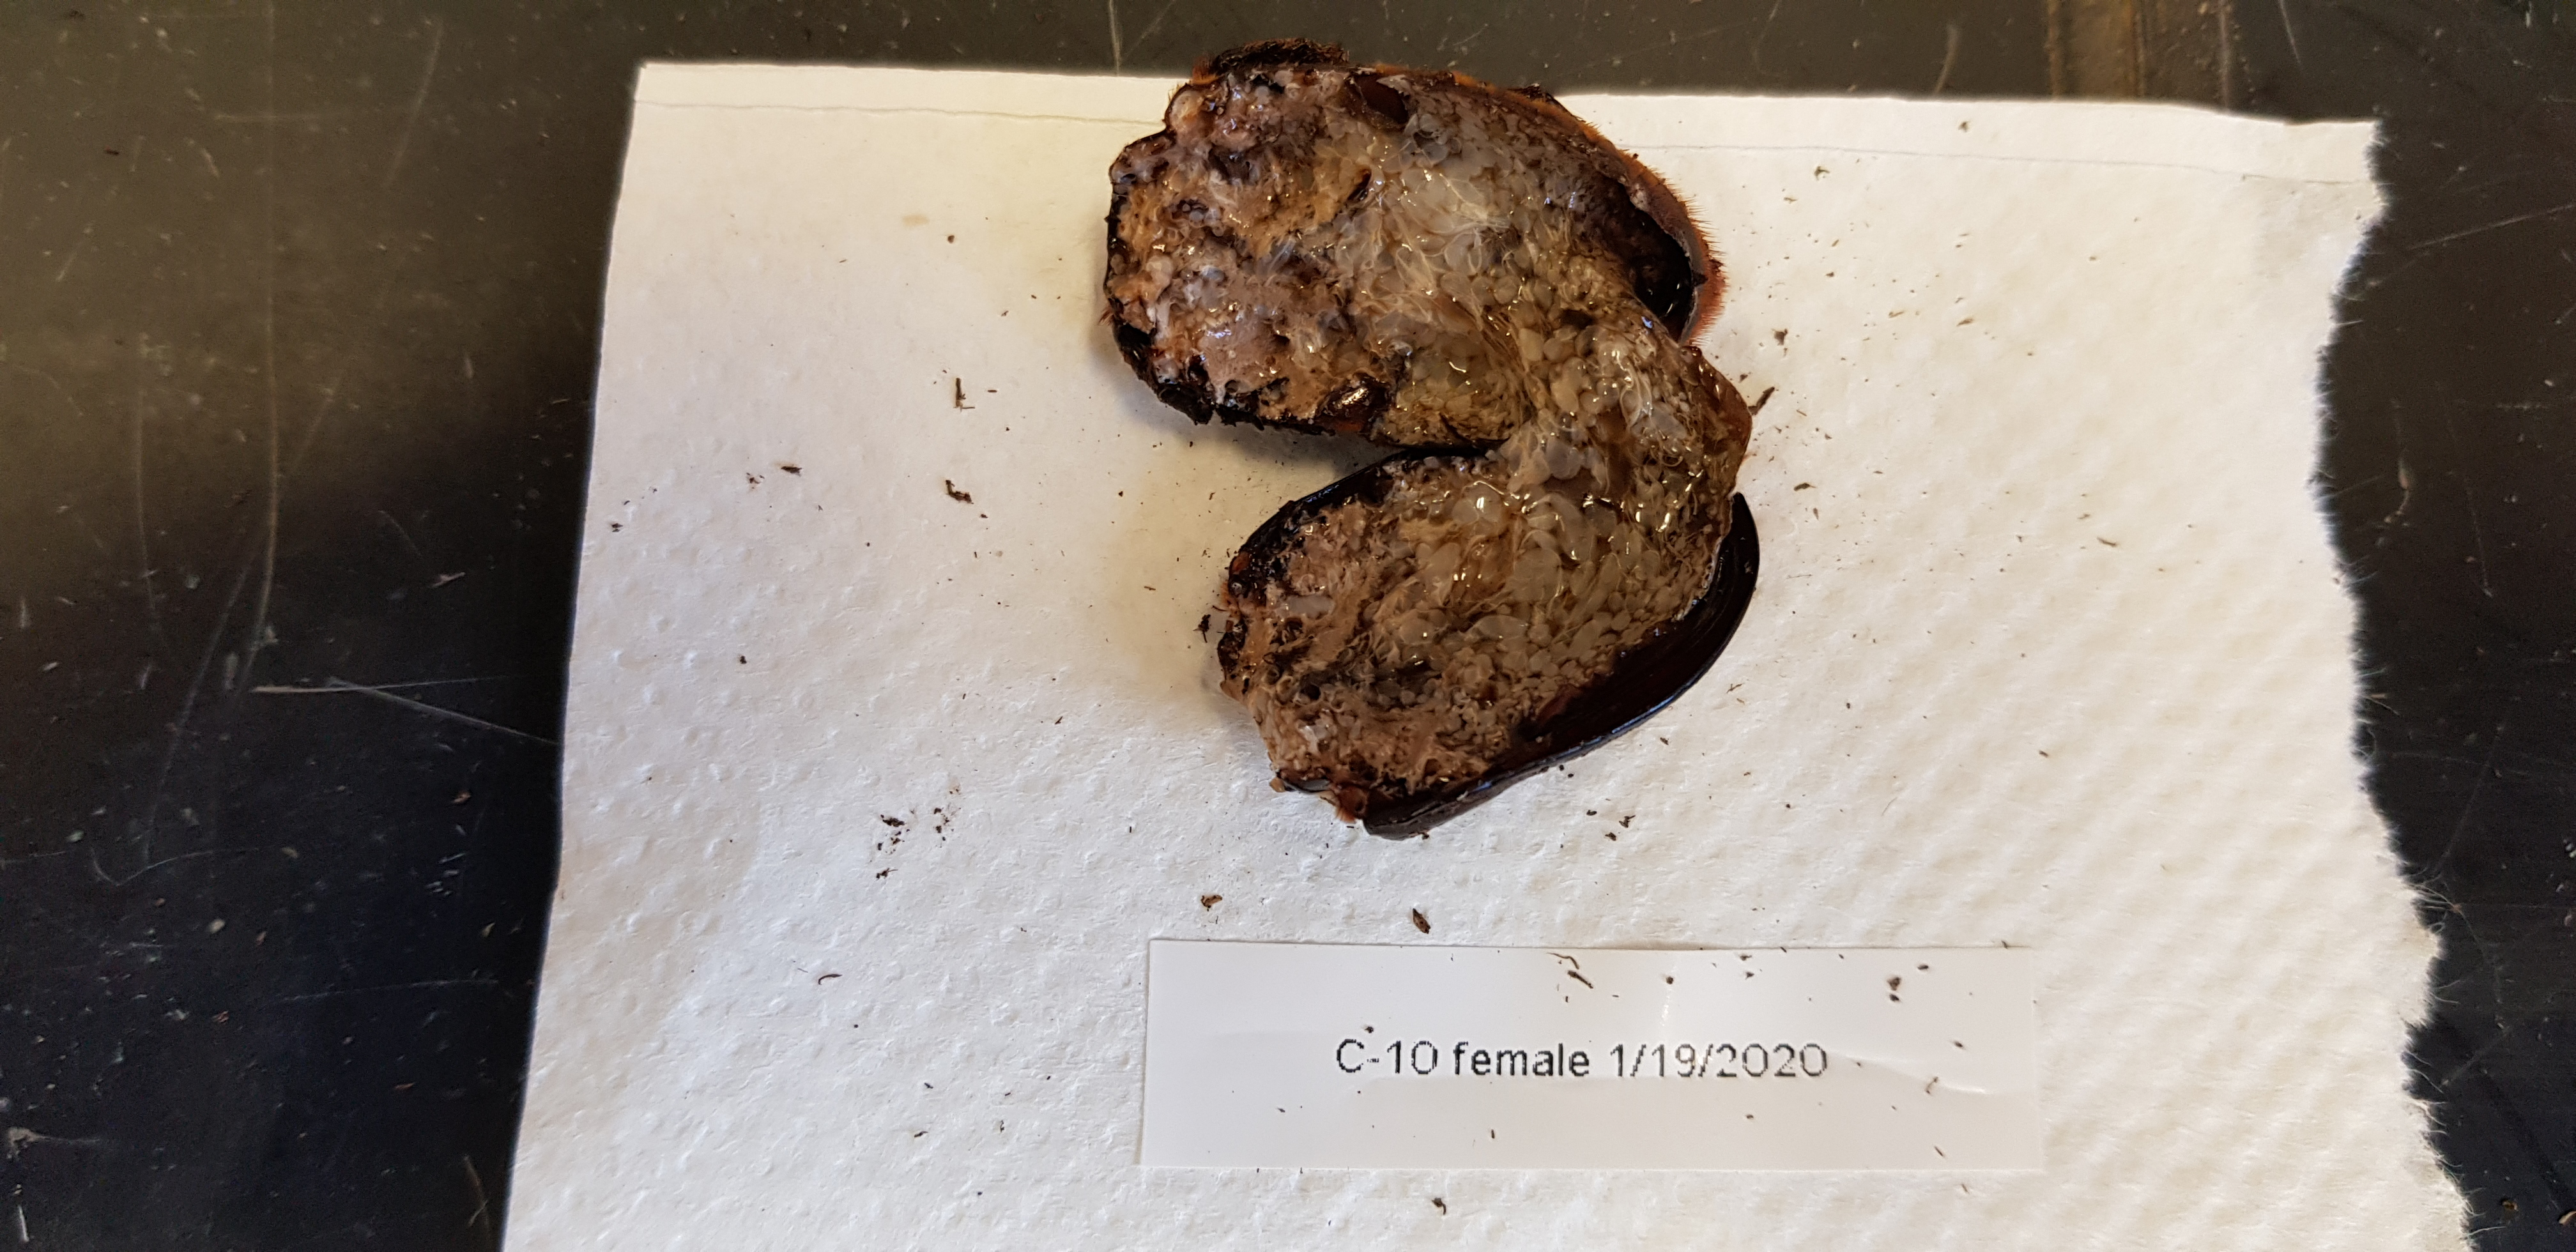
\includegraphics[width=\textwidth]{pm-images/20200119_121825.jpg}
\caption{\textbf{C10f} jar\_id                                 C10
sex                                      f
treatment                             none
date\_treated           2019-12-27 00:00:00
date\_died              2020-01-19 00:00:00
postmortem\_virus                       NaN
postmortem\_bacteria                    NaN
pm\_image\_filename      20200119\_121825.jpg
date\_end\_bioassay      2020-02-06 00:00:00
t                                       23
e                                     True
Name: 24, dtype: object}
\end{figure}
\clearpage

\begin{figure}[h!]
\centering
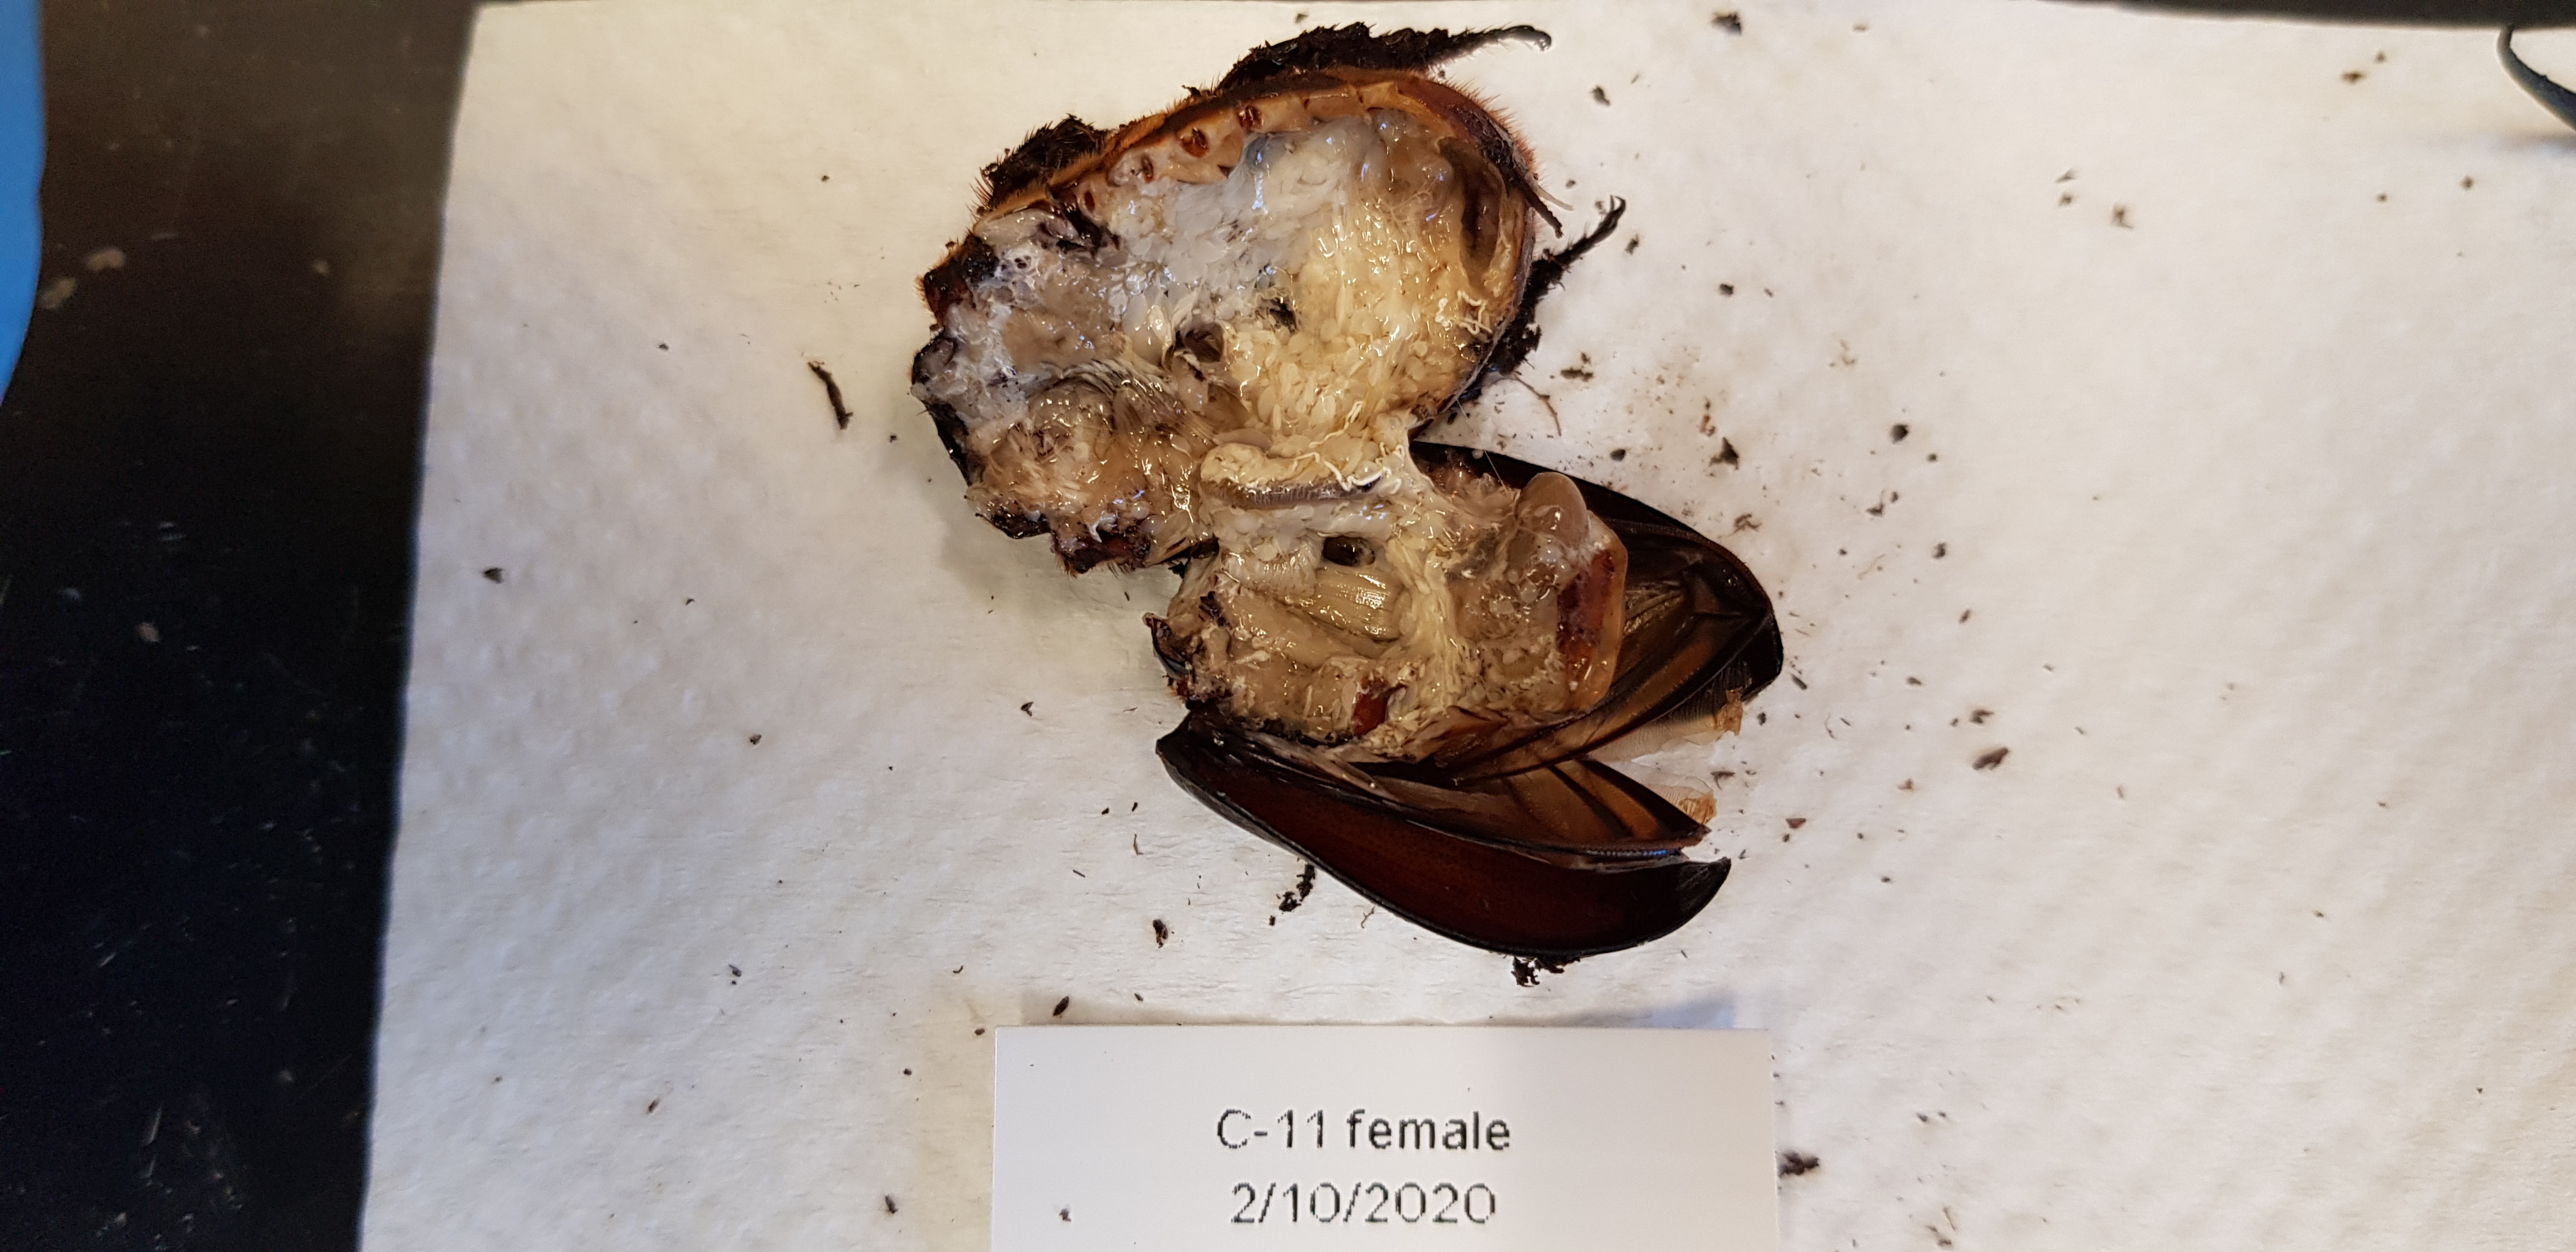
\includegraphics[width=\textwidth]{pm-images/20200210_151339.jpg}
\caption{\textbf{C11f} jar\_id                                 C11
sex                                      f
treatment                             none
date\_treated           2019-12-27 00:00:00
date\_died                              NaT
postmortem\_virus                       NaN
postmortem\_bacteria                    NaN
pm\_image\_filename      20200210\_151339.jpg
date\_end\_bioassay      2020-02-06 00:00:00
t                                       41
e                                    False
Name: 25, dtype: object}
\end{figure}
\clearpage

\begin{figure}[h!]
\centering
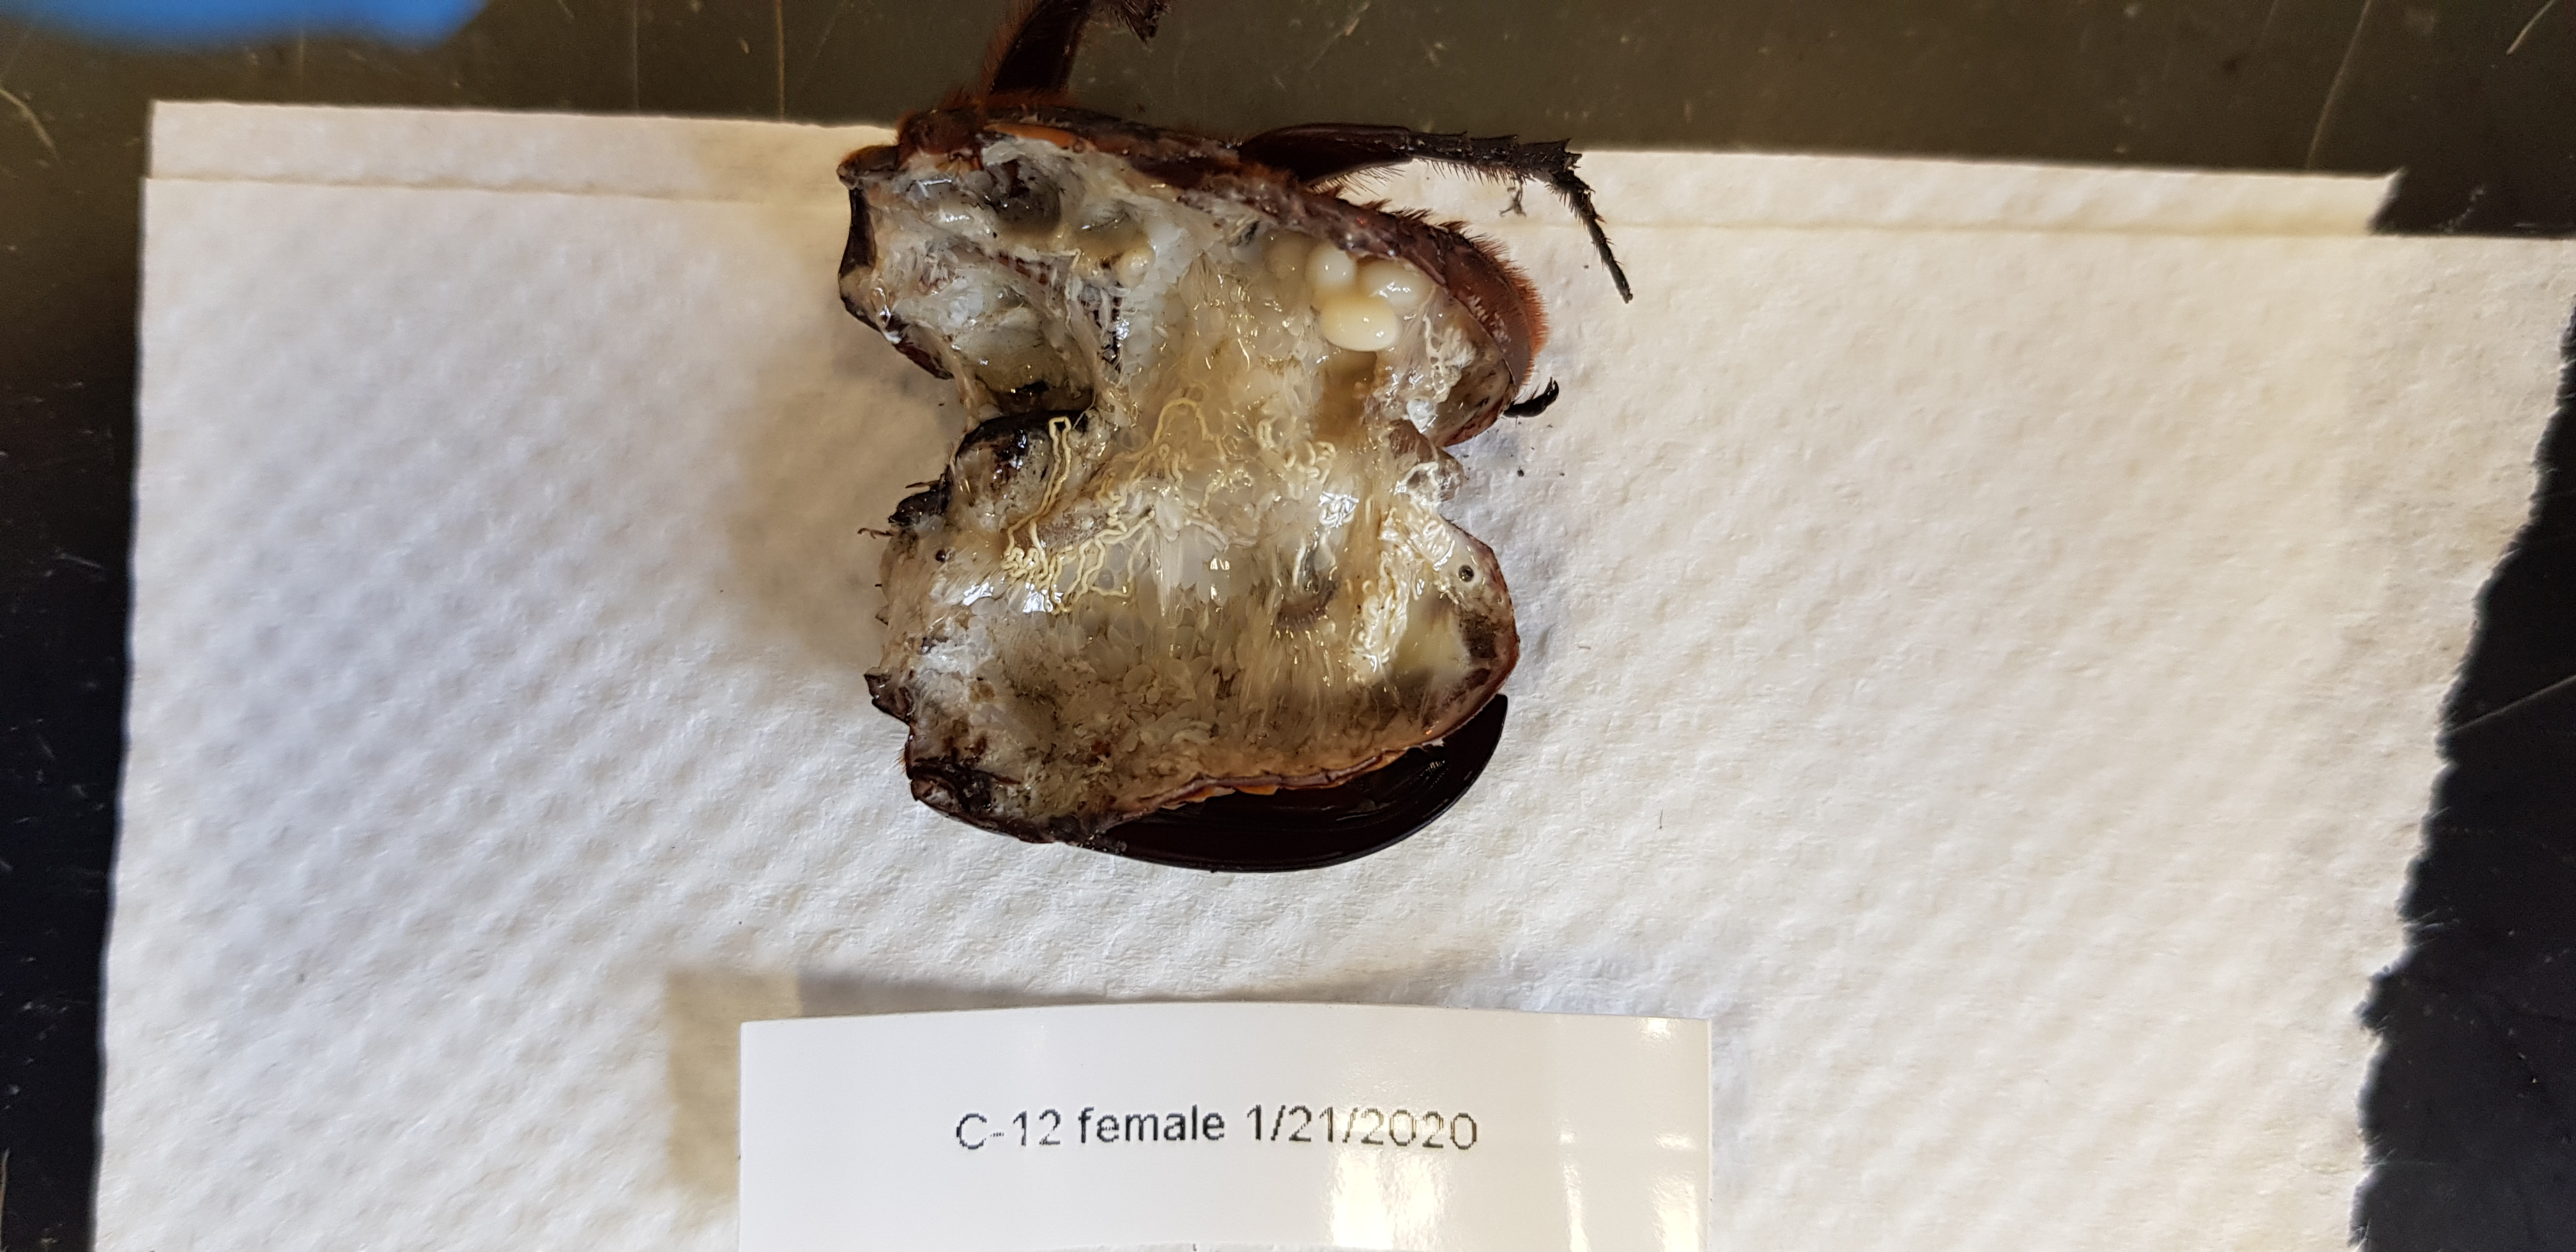
\includegraphics[width=\textwidth]{pm-images/20200121_113027.jpg}
\caption{\textbf{C12f} jar\_id                                 C12
sex                                      f
treatment                             none
date\_treated           2019-12-27 00:00:00
date\_died              2020-01-21 00:00:00
postmortem\_virus                       NaN
postmortem\_bacteria                    NaN
pm\_image\_filename      20200121\_113027.jpg
date\_end\_bioassay      2020-02-06 00:00:00
t                                       25
e                                     True
Name: 26, dtype: object}
\end{figure}
\clearpage

\begin{figure}[h!]
\centering
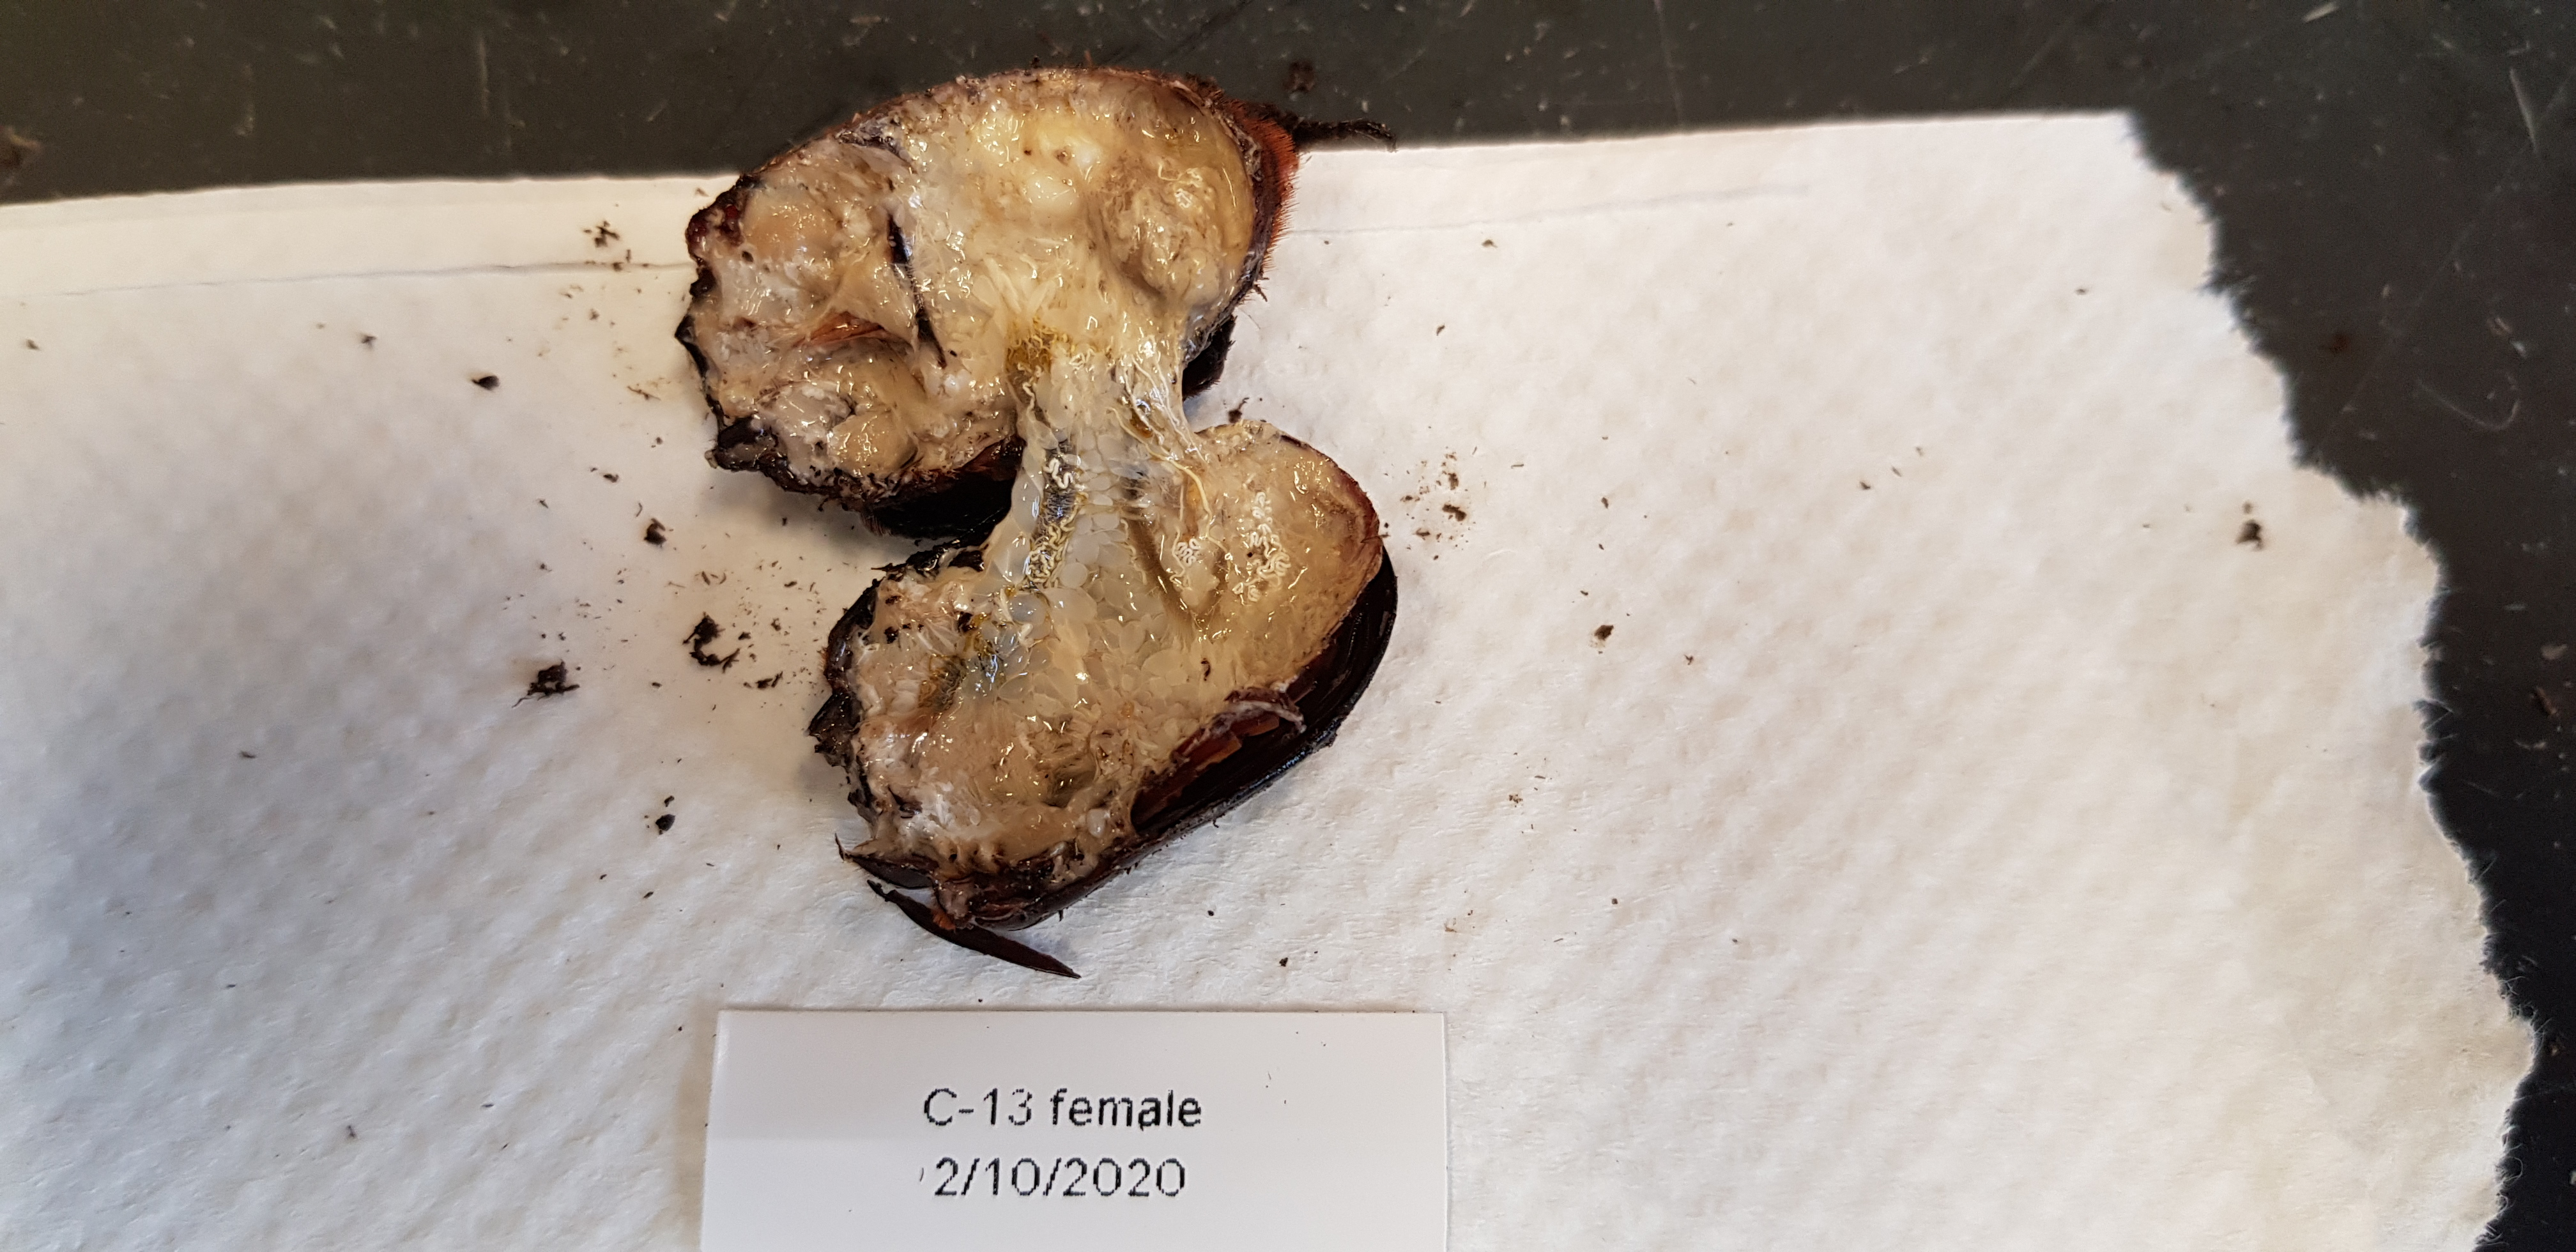
\includegraphics[width=\textwidth]{pm-images/20200210_152419.jpg}
\caption{\textbf{C13f} jar\_id                                 C13
sex                                      f
treatment                             none
date\_treated           2019-12-27 00:00:00
date\_died                              NaT
postmortem\_virus                       NaN
postmortem\_bacteria                    NaN
pm\_image\_filename      20200210\_152419.jpg
date\_end\_bioassay      2020-02-06 00:00:00
t                                       41
e                                    False
Name: 27, dtype: object}
\end{figure}
\clearpage

\begin{figure}[h!]
\centering
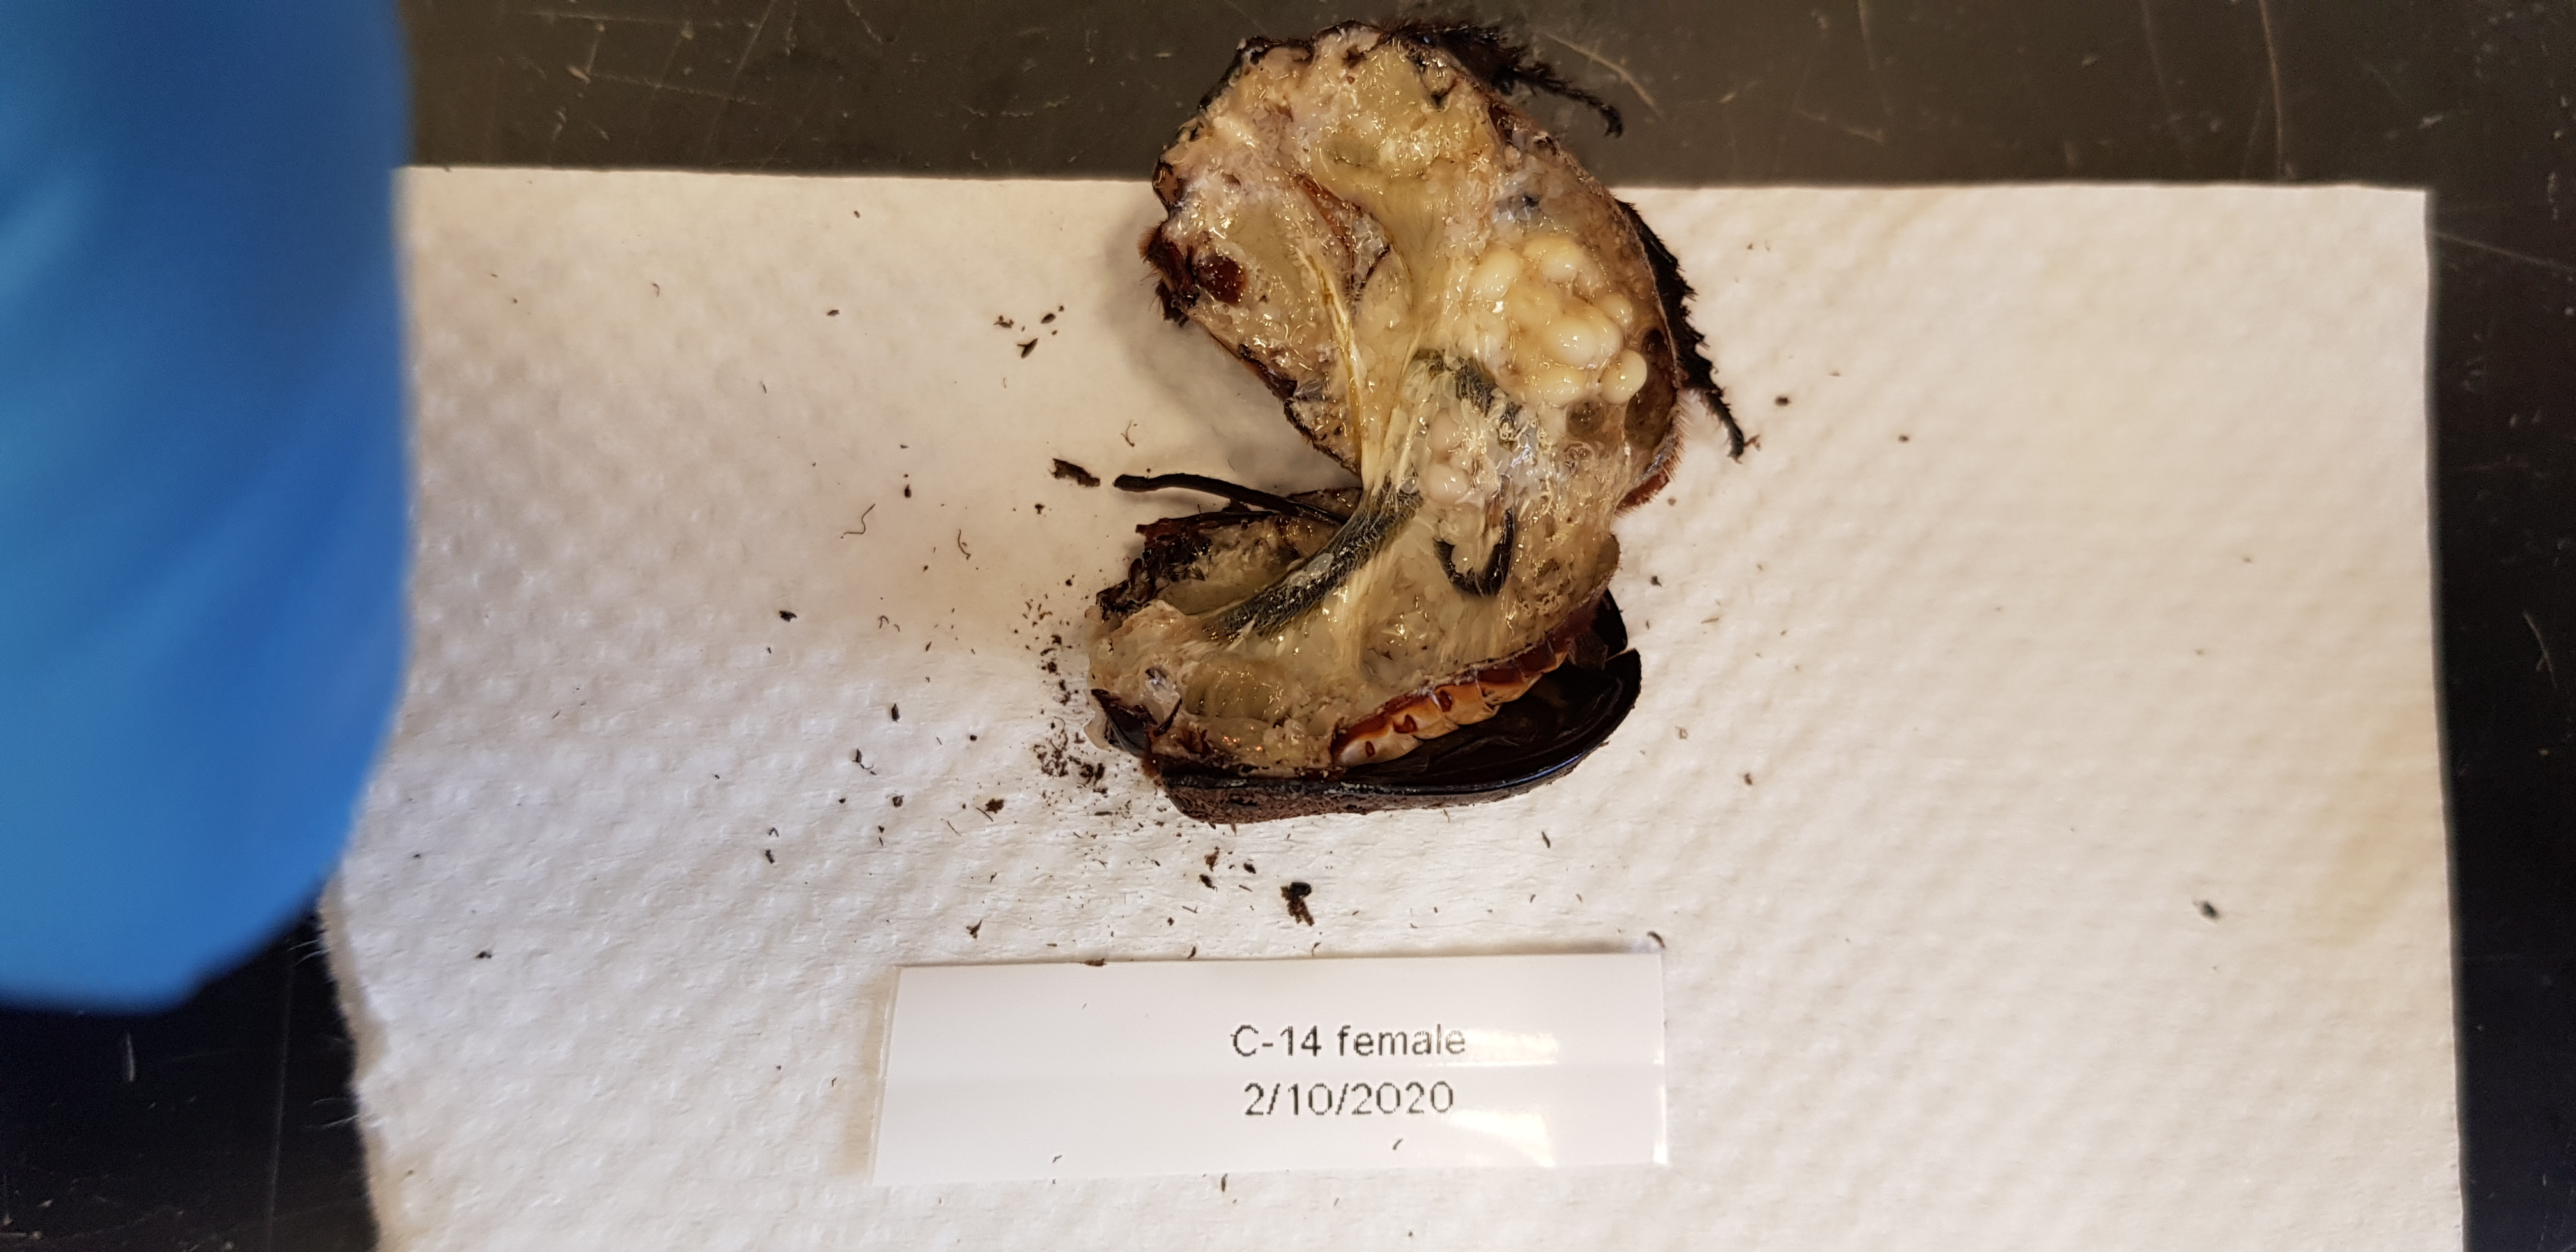
\includegraphics[width=\textwidth]{pm-images/20200210_145811.jpg}
\caption{\textbf{C14f} jar\_id                                 C14
sex                                      f
treatment                             none
date\_treated           2019-12-27 00:00:00
date\_died                              NaT
postmortem\_virus                       NaN
postmortem\_bacteria                    NaN
pm\_image\_filename      20200210\_145811.jpg
date\_end\_bioassay      2020-02-06 00:00:00
t                                       41
e                                    False
Name: 28, dtype: object}
\end{figure}
\clearpage

\begin{figure}[h!]
\centering
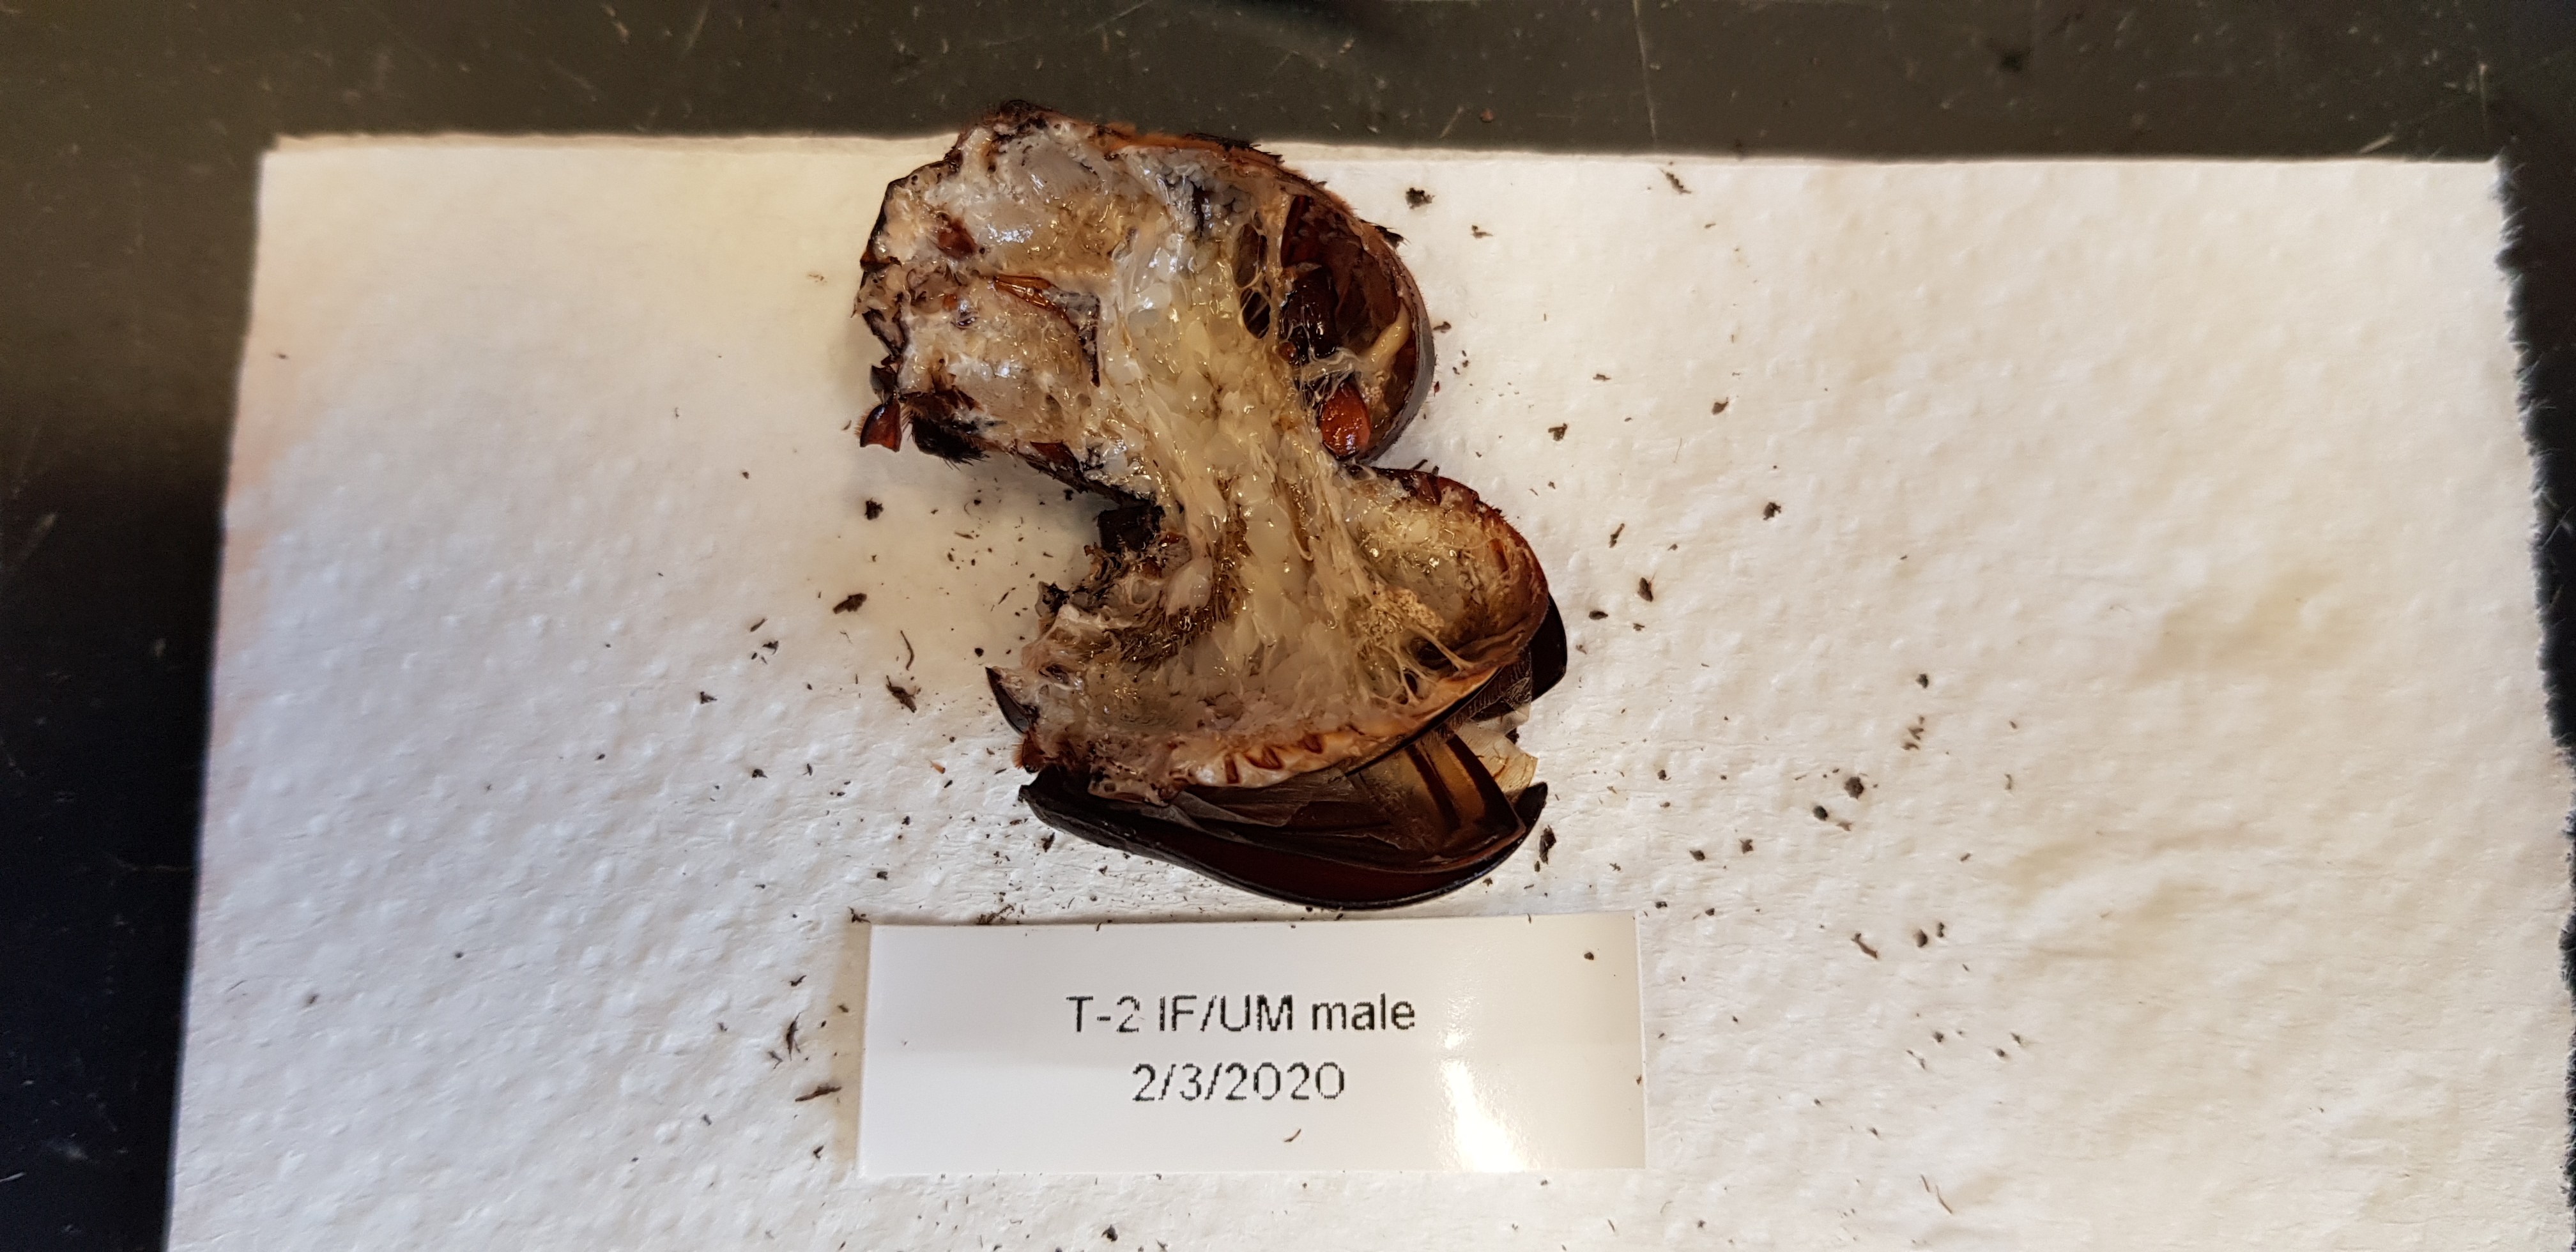
\includegraphics[width=\textwidth]{pm-images/20200203_114327.jpg}
\caption{\textbf{TF2m} jar\_id                                 TF2
sex                                      m
treatment                        companion
date\_treated           2019-12-26 00:00:00
date\_died              2020-02-03 00:00:00
postmortem\_virus                       NaN
postmortem\_bacteria                    NaN
pm\_image\_filename      20200203\_114327.jpg
date\_end\_bioassay      2020-02-06 00:00:00
t                                       39
e                                     True
Name: 31, dtype: object}
\end{figure}
\clearpage

\begin{figure}[h!]
\centering
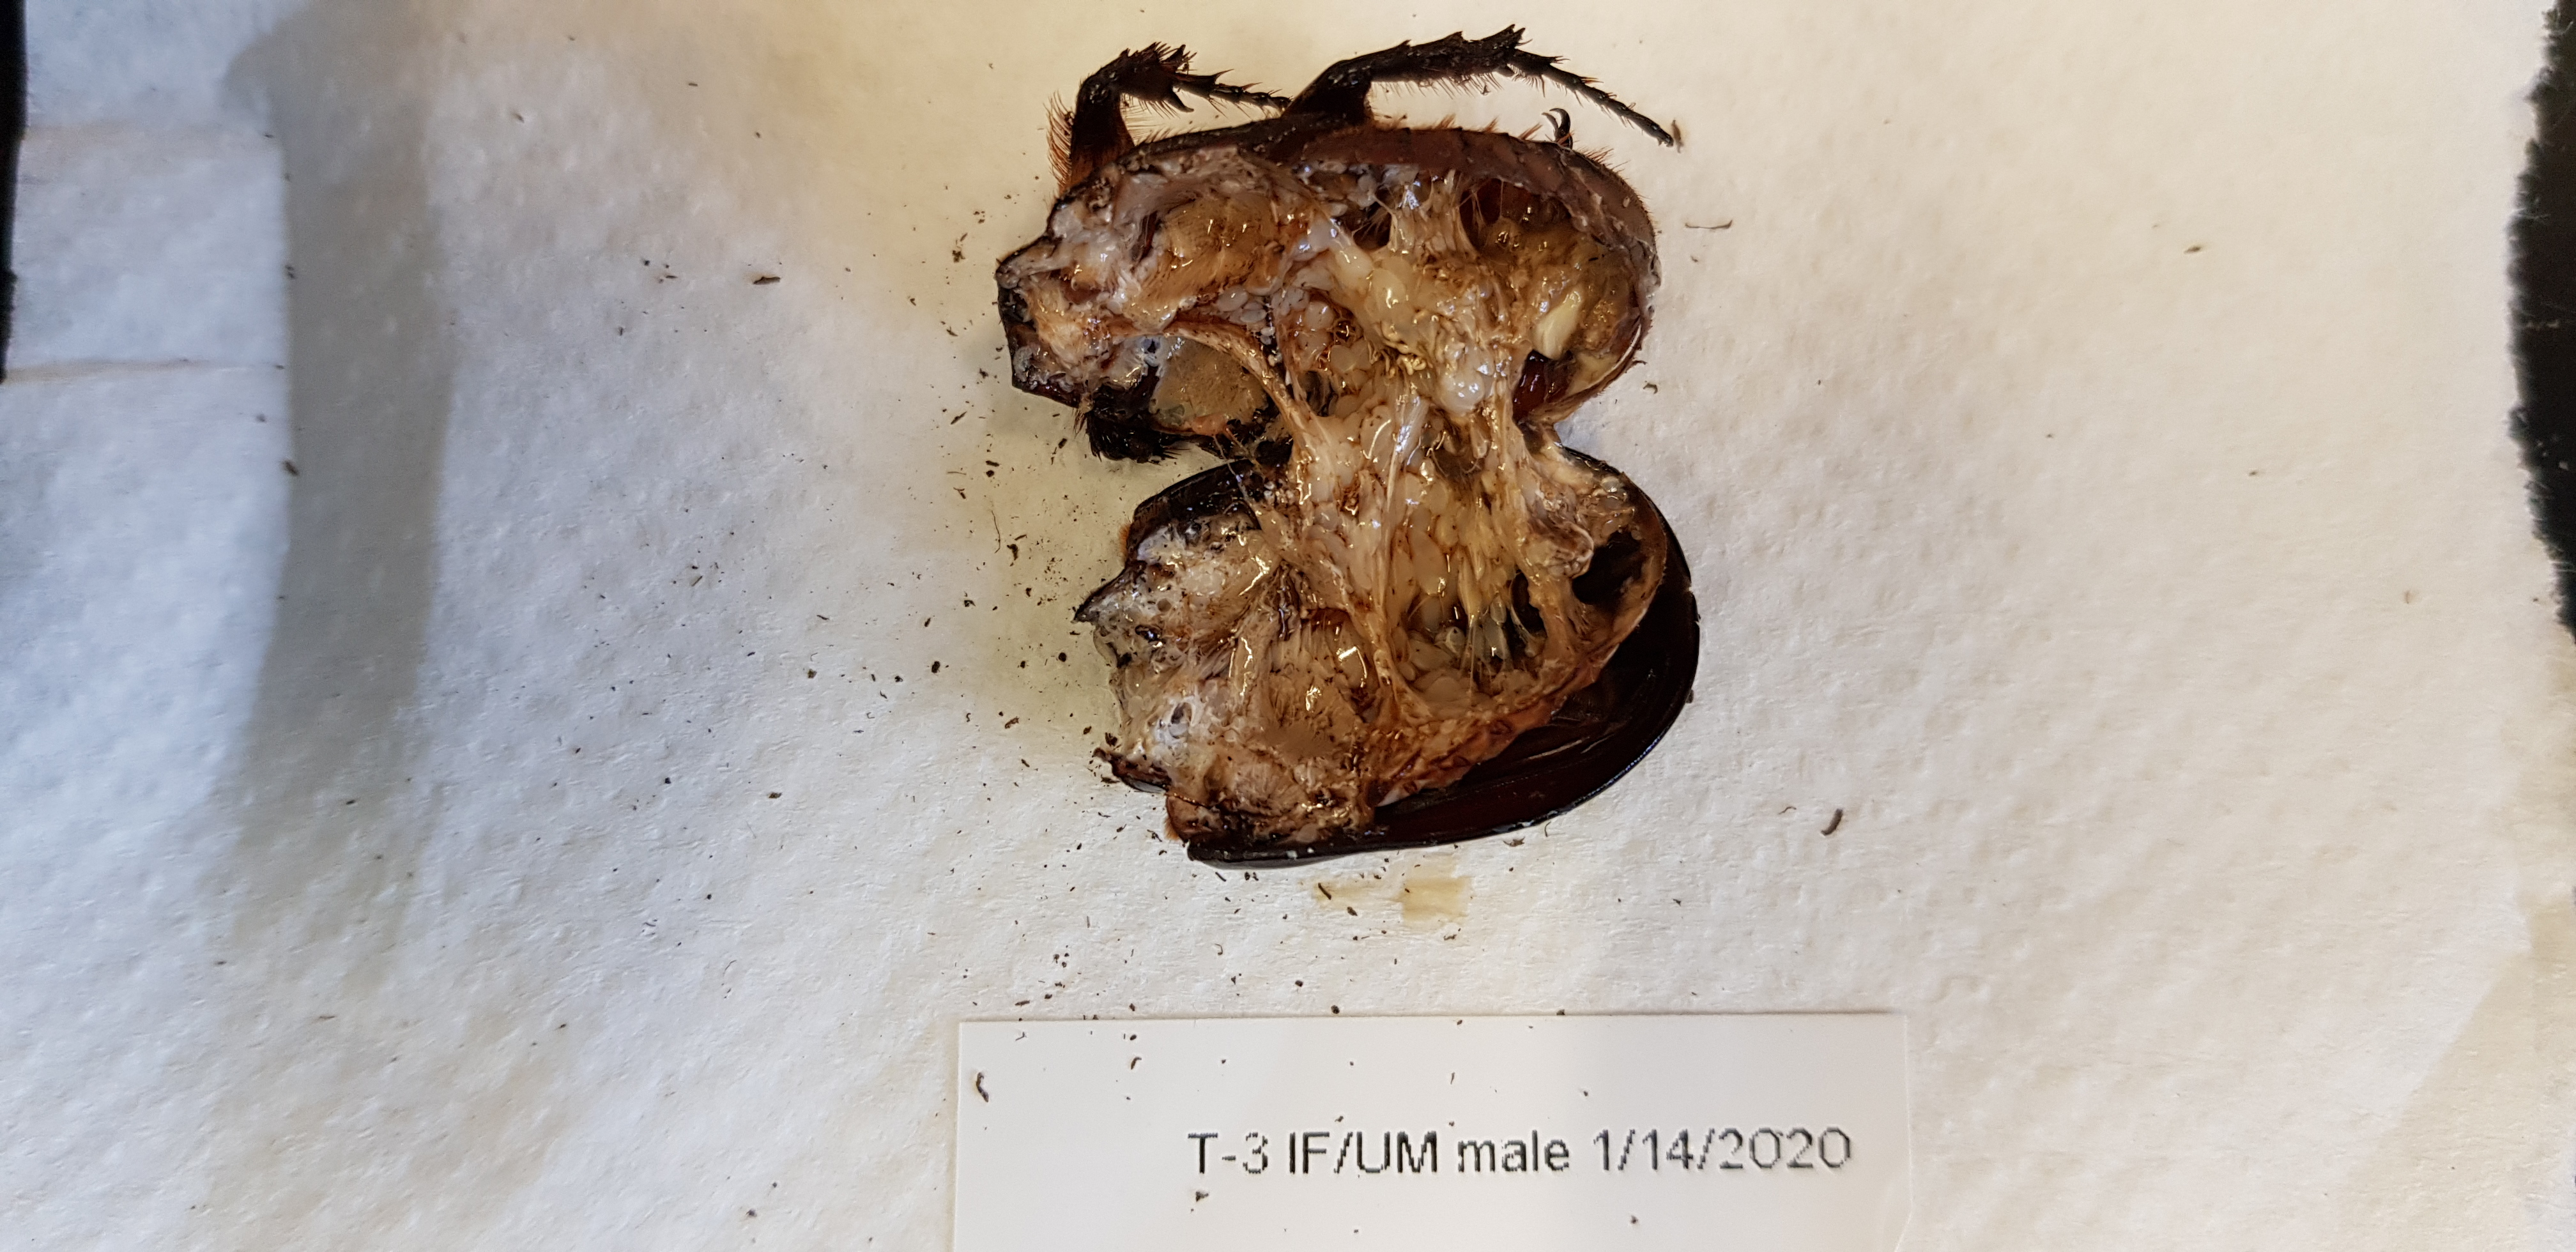
\includegraphics[width=\textwidth]{pm-images/20200114_104530.jpg}
\caption{\textbf{TF3m} jar\_id                                 TF3
sex                                      m
treatment                        companion
date\_treated           2019-12-26 00:00:00
date\_died              2020-01-19 00:00:00
postmortem\_virus                       NaN
postmortem\_bacteria                      1
pm\_image\_filename      20200114\_104530.jpg
date\_end\_bioassay      2020-02-06 00:00:00
t                                       24
e                                     True
Name: 32, dtype: object}
\end{figure}
\clearpage

\begin{figure}[h!]
\centering
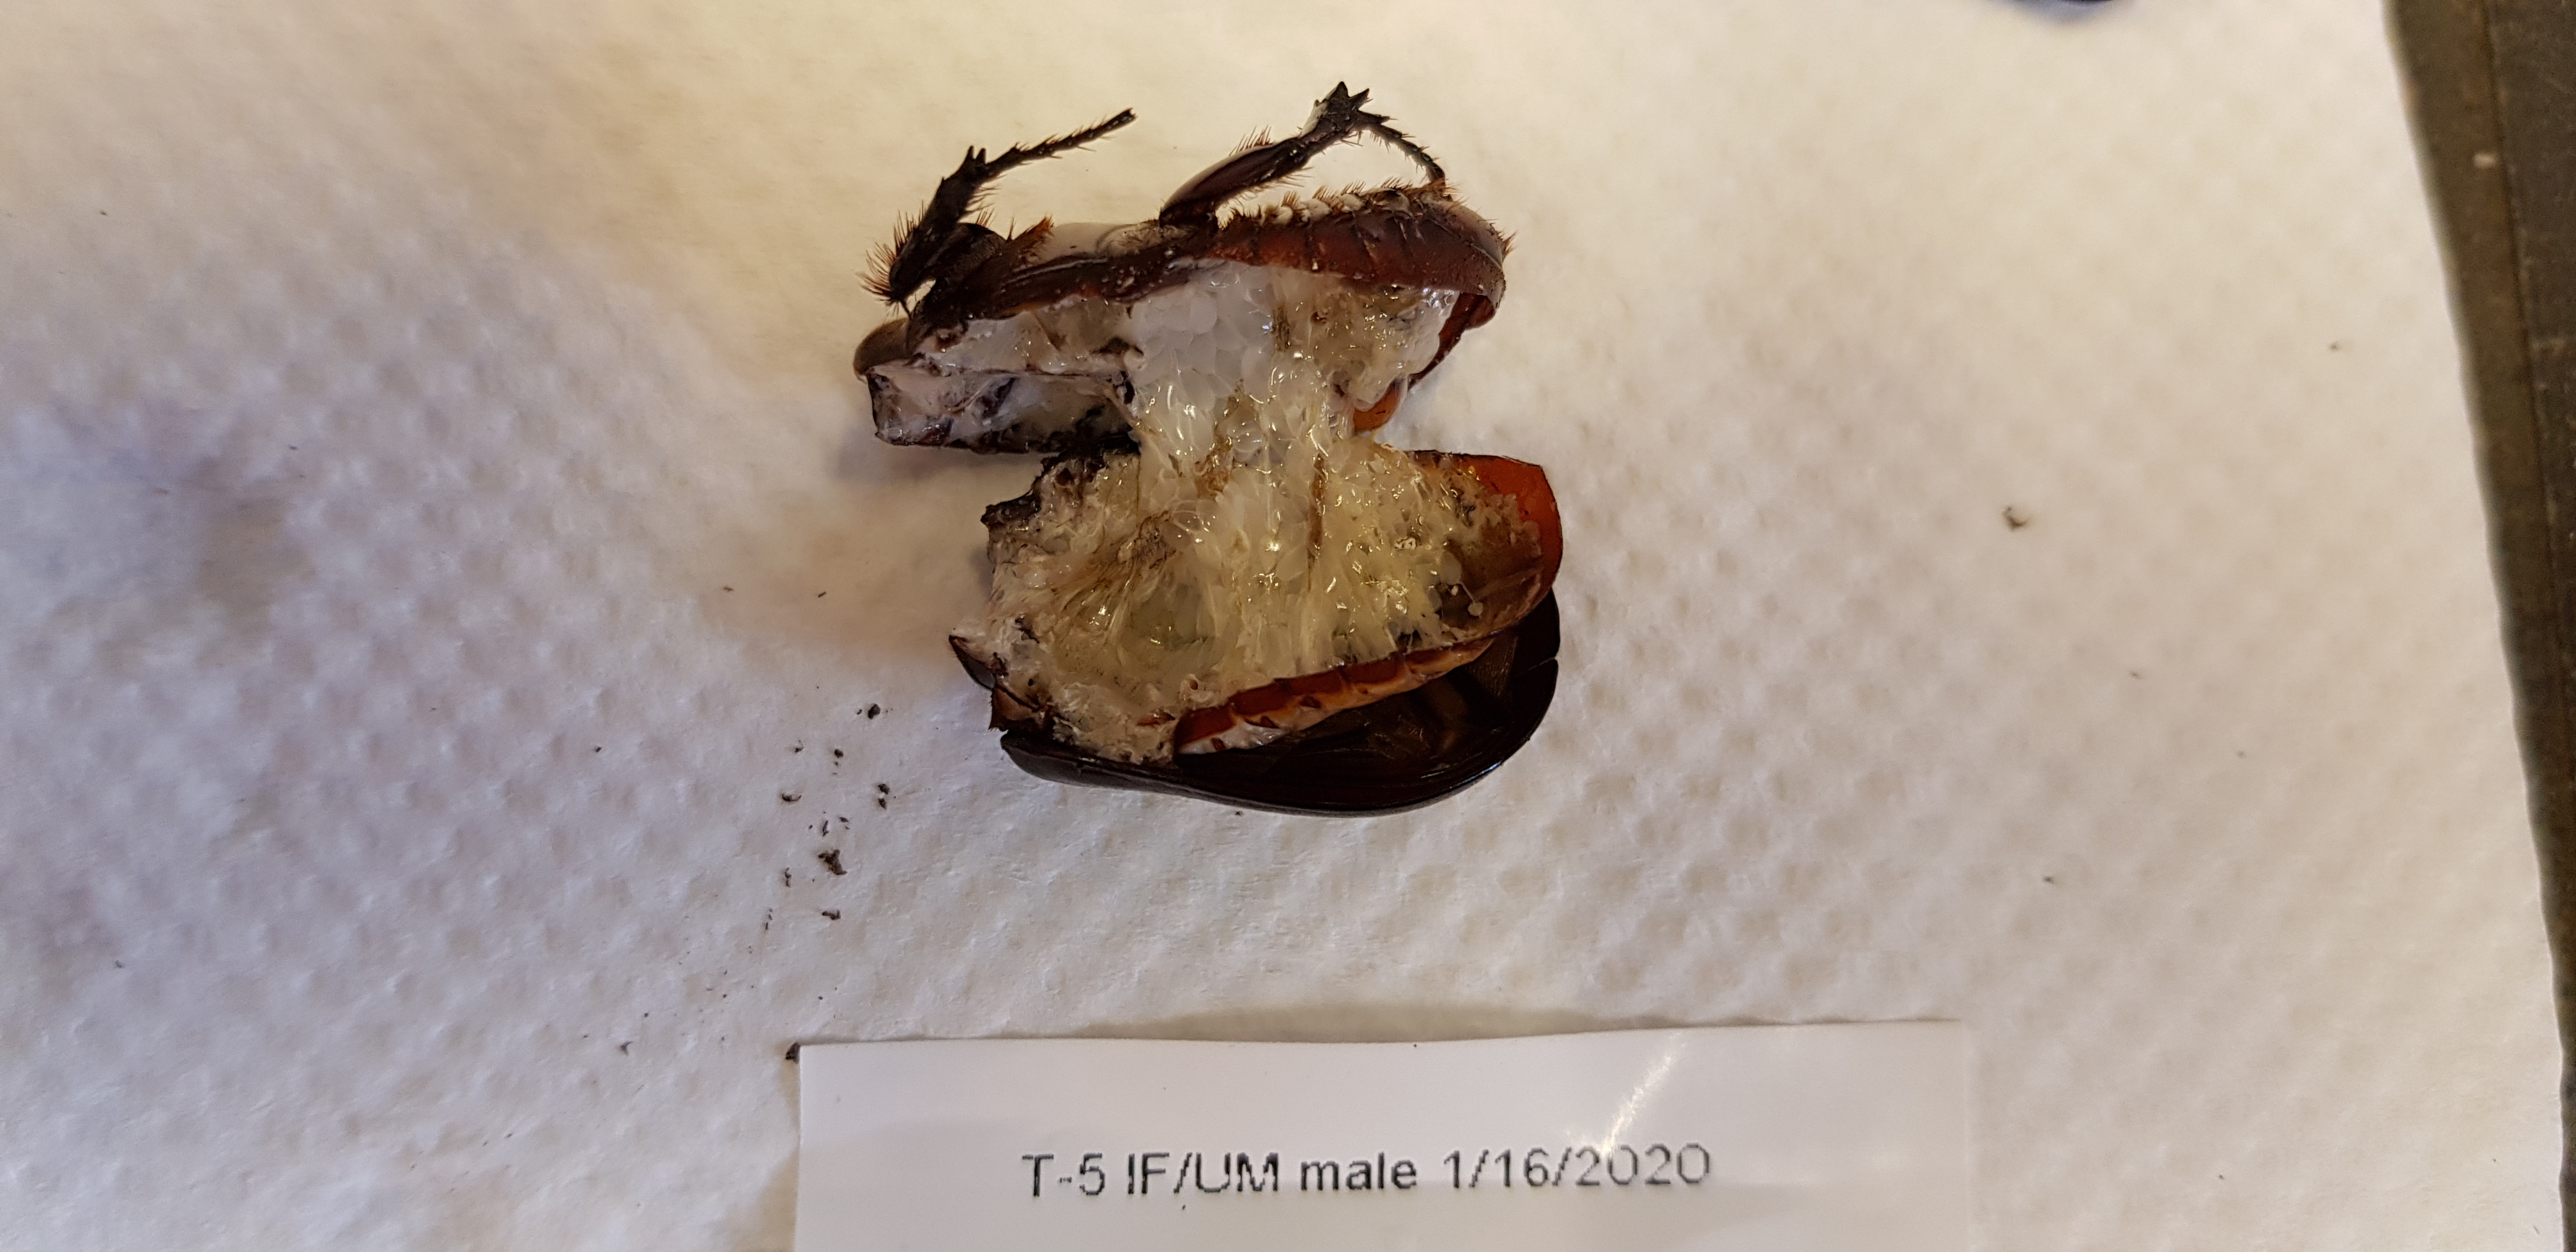
\includegraphics[width=\textwidth]{pm-images/20200116_111311.jpg}
\caption{\textbf{TF5m} jar\_id                                 TF5
sex                                      m
treatment                        companion
date\_treated           2019-12-26 00:00:00
date\_died              2020-01-16 00:00:00
postmortem\_virus                       NaN
postmortem\_bacteria                    NaN
pm\_image\_filename      20200116\_111311.jpg
date\_end\_bioassay      2020-02-06 00:00:00
t                                       21
e                                     True
Name: 34, dtype: object}
\end{figure}
\clearpage

\begin{figure}[h!]
\centering
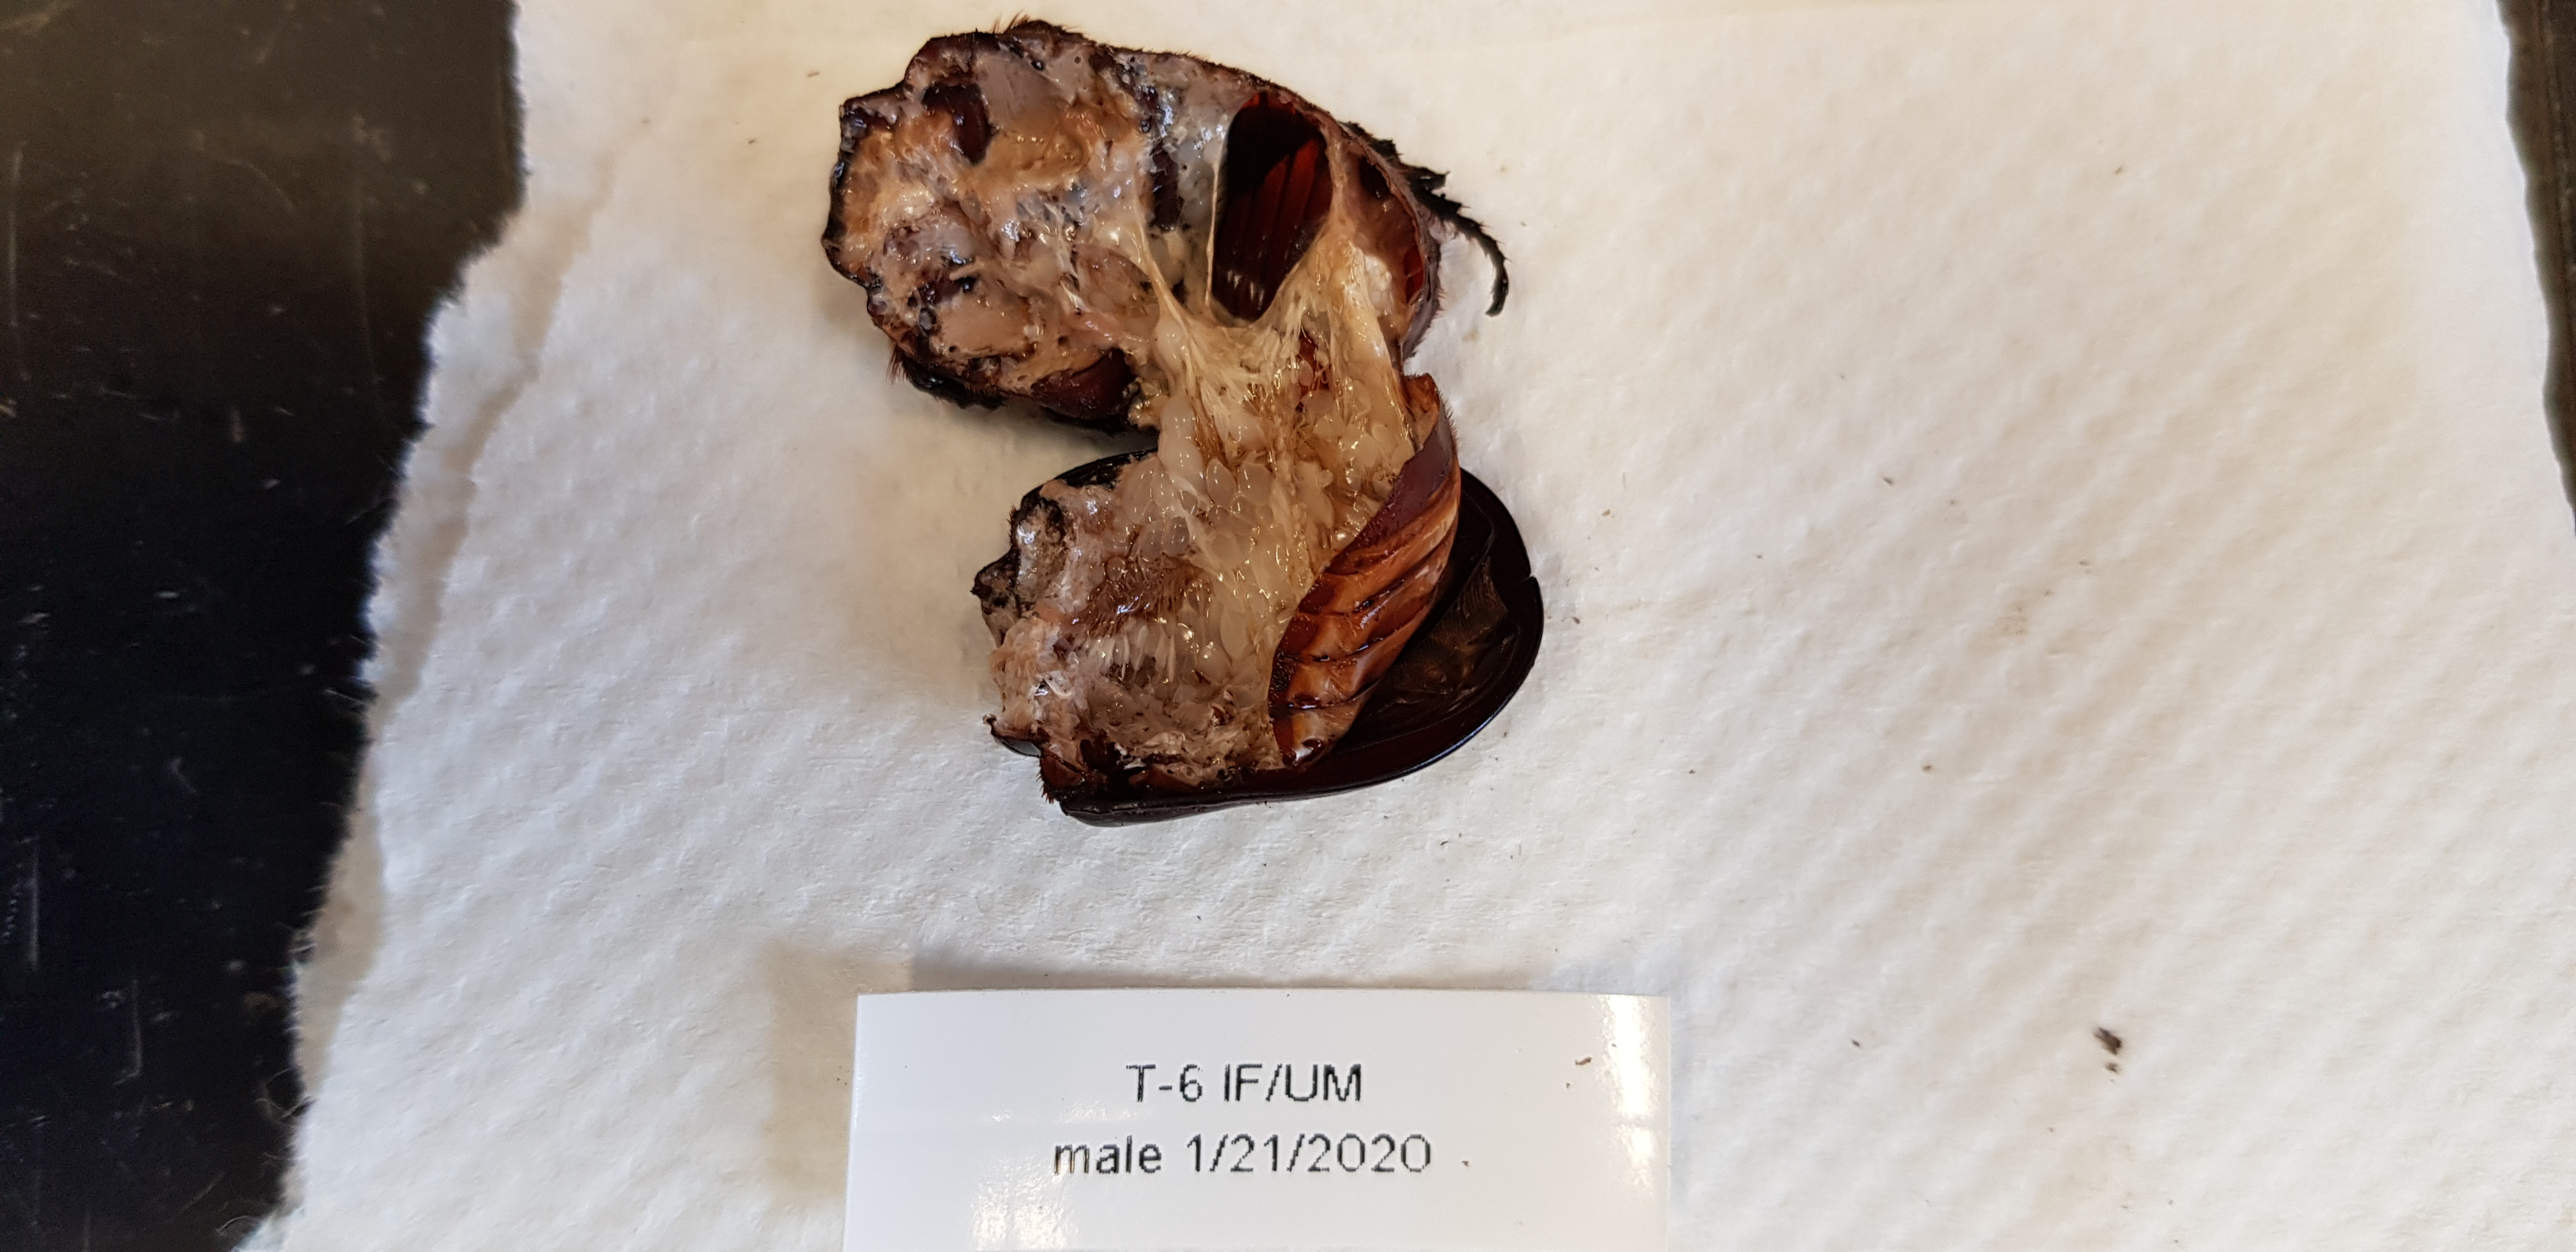
\includegraphics[width=\textwidth]{pm-images/20200121_111727.jpg}
\caption{\textbf{TF6m} jar\_id                                 TF6
sex                                      m
treatment                        companion
date\_treated           2019-12-27 00:00:00
date\_died              2020-01-21 00:00:00
postmortem\_virus                       NaN
postmortem\_bacteria                      1
pm\_image\_filename      20200121\_111727.jpg
date\_end\_bioassay      2020-02-06 00:00:00
t                                       25
e                                     True
Name: 35, dtype: object}
\end{figure}
\clearpage

\begin{figure}[h!]
\centering
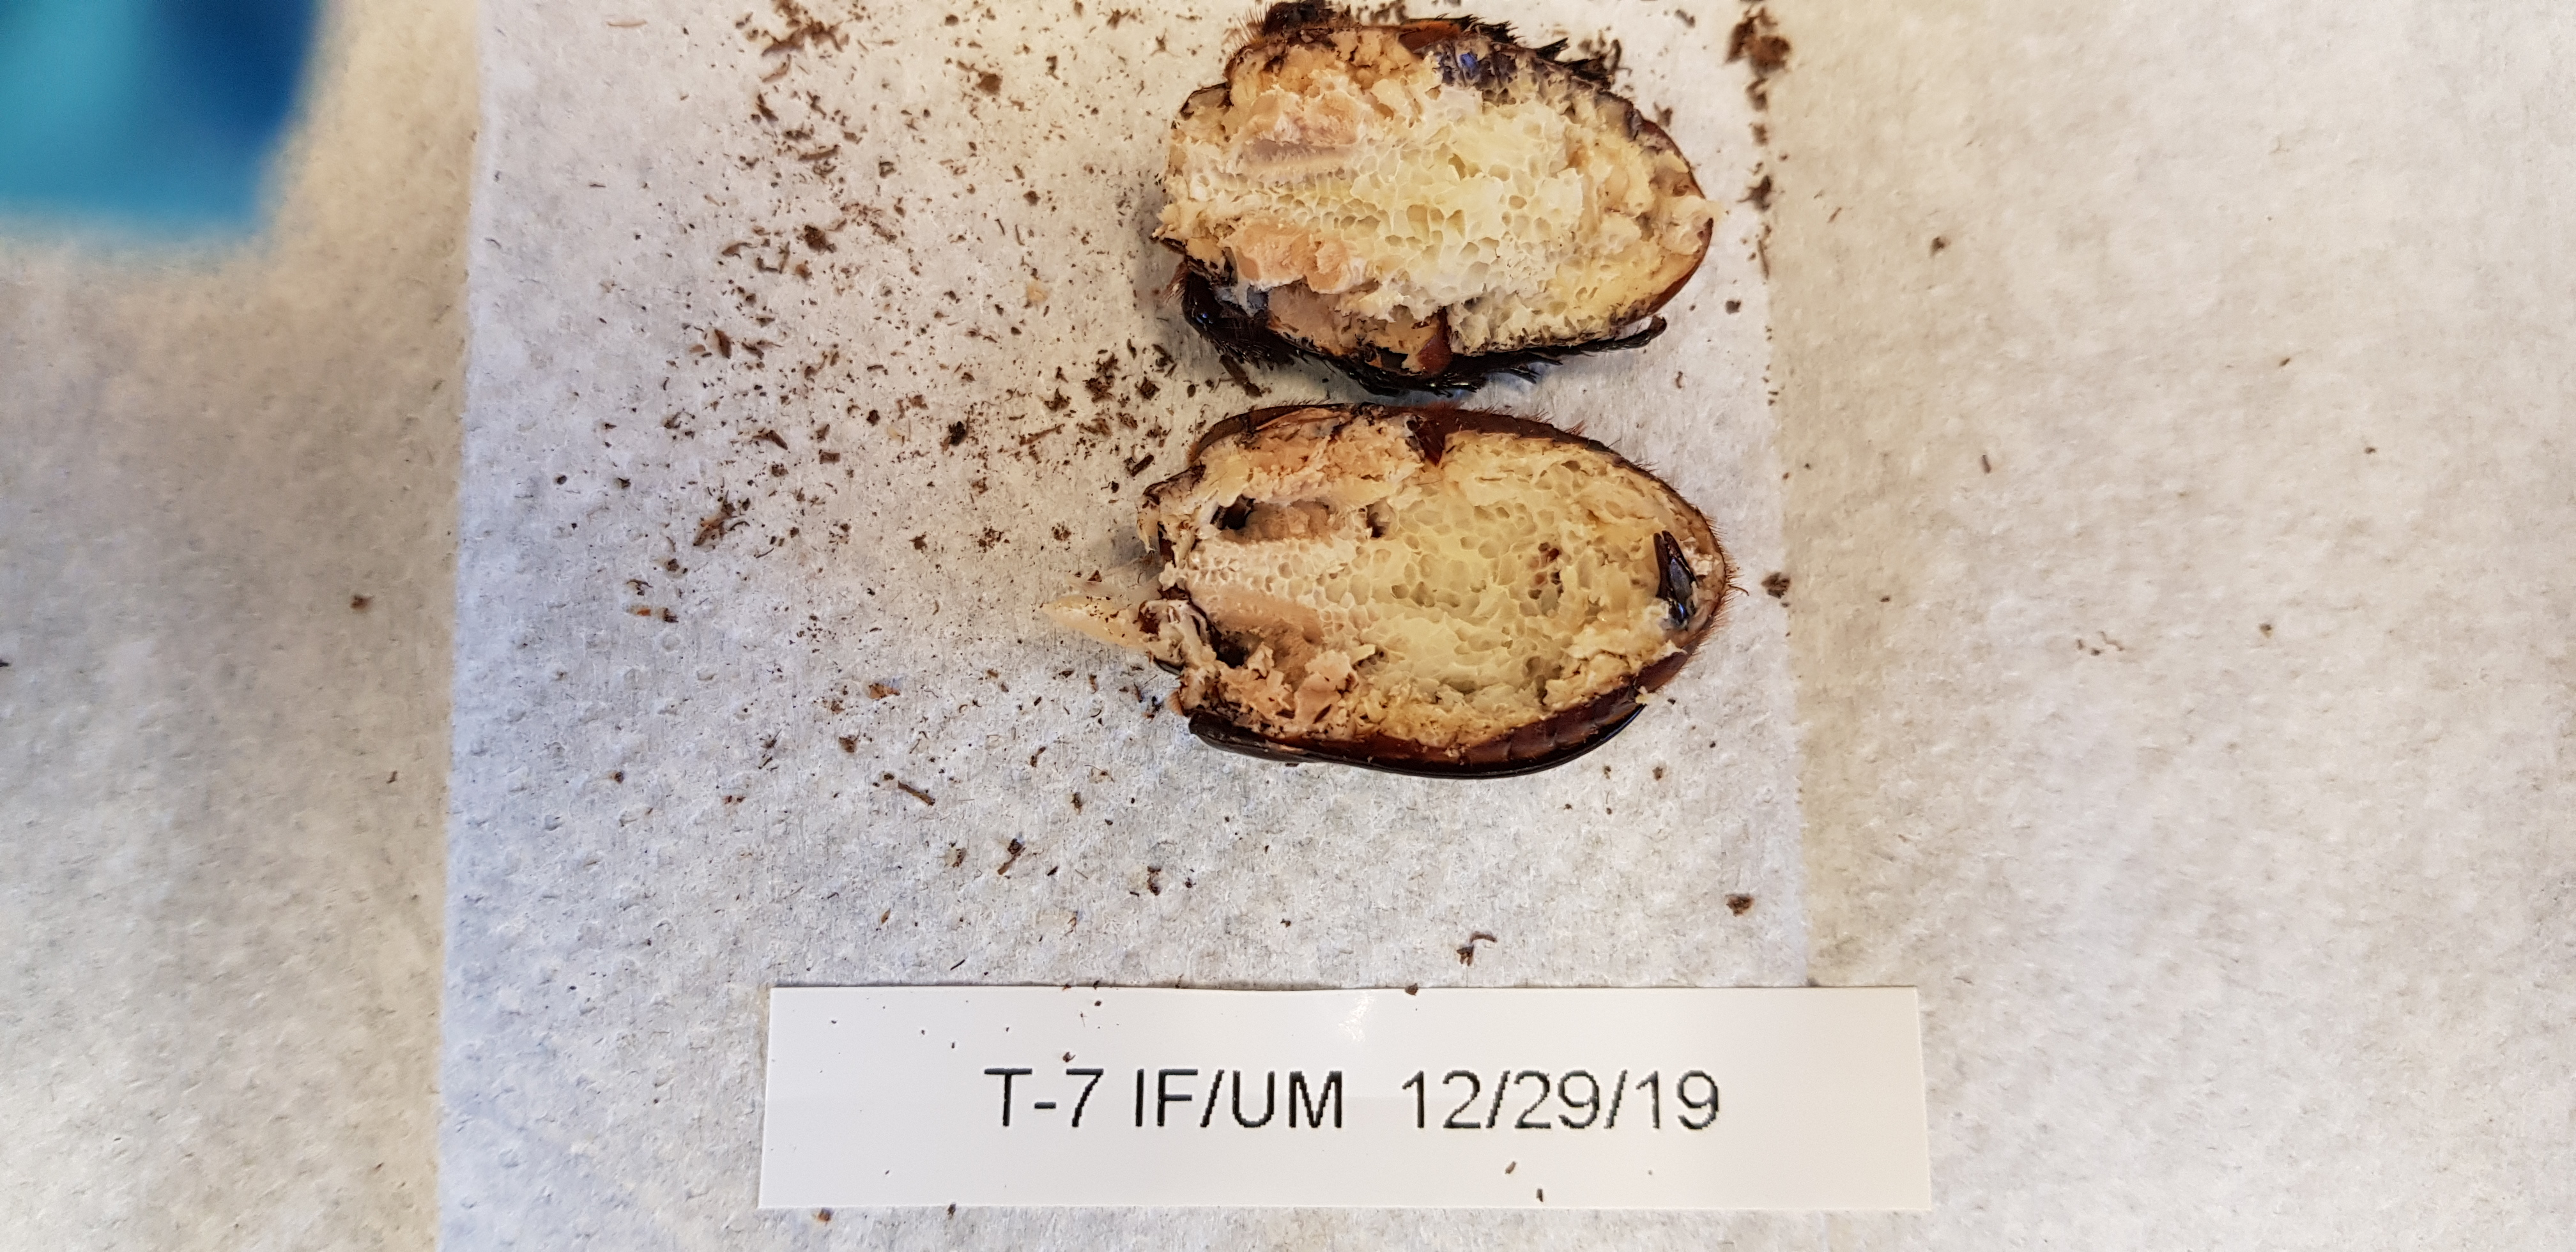
\includegraphics[width=\textwidth]{pm-images/20191229_120148.jpg}
\caption{\textbf{TF7m} jar\_id                                 TF7
sex                                      m
treatment                        companion
date\_treated           2019-12-27 00:00:00
date\_died              2020-01-27 00:00:00
postmortem\_virus                       NaN
postmortem\_bacteria                      1
pm\_image\_filename      20191229\_120148.jpg
date\_end\_bioassay      2020-02-06 00:00:00
t                                       31
e                                     True
Name: 36, dtype: object}
\end{figure}
\clearpage

\begin{figure}[h!]
\centering
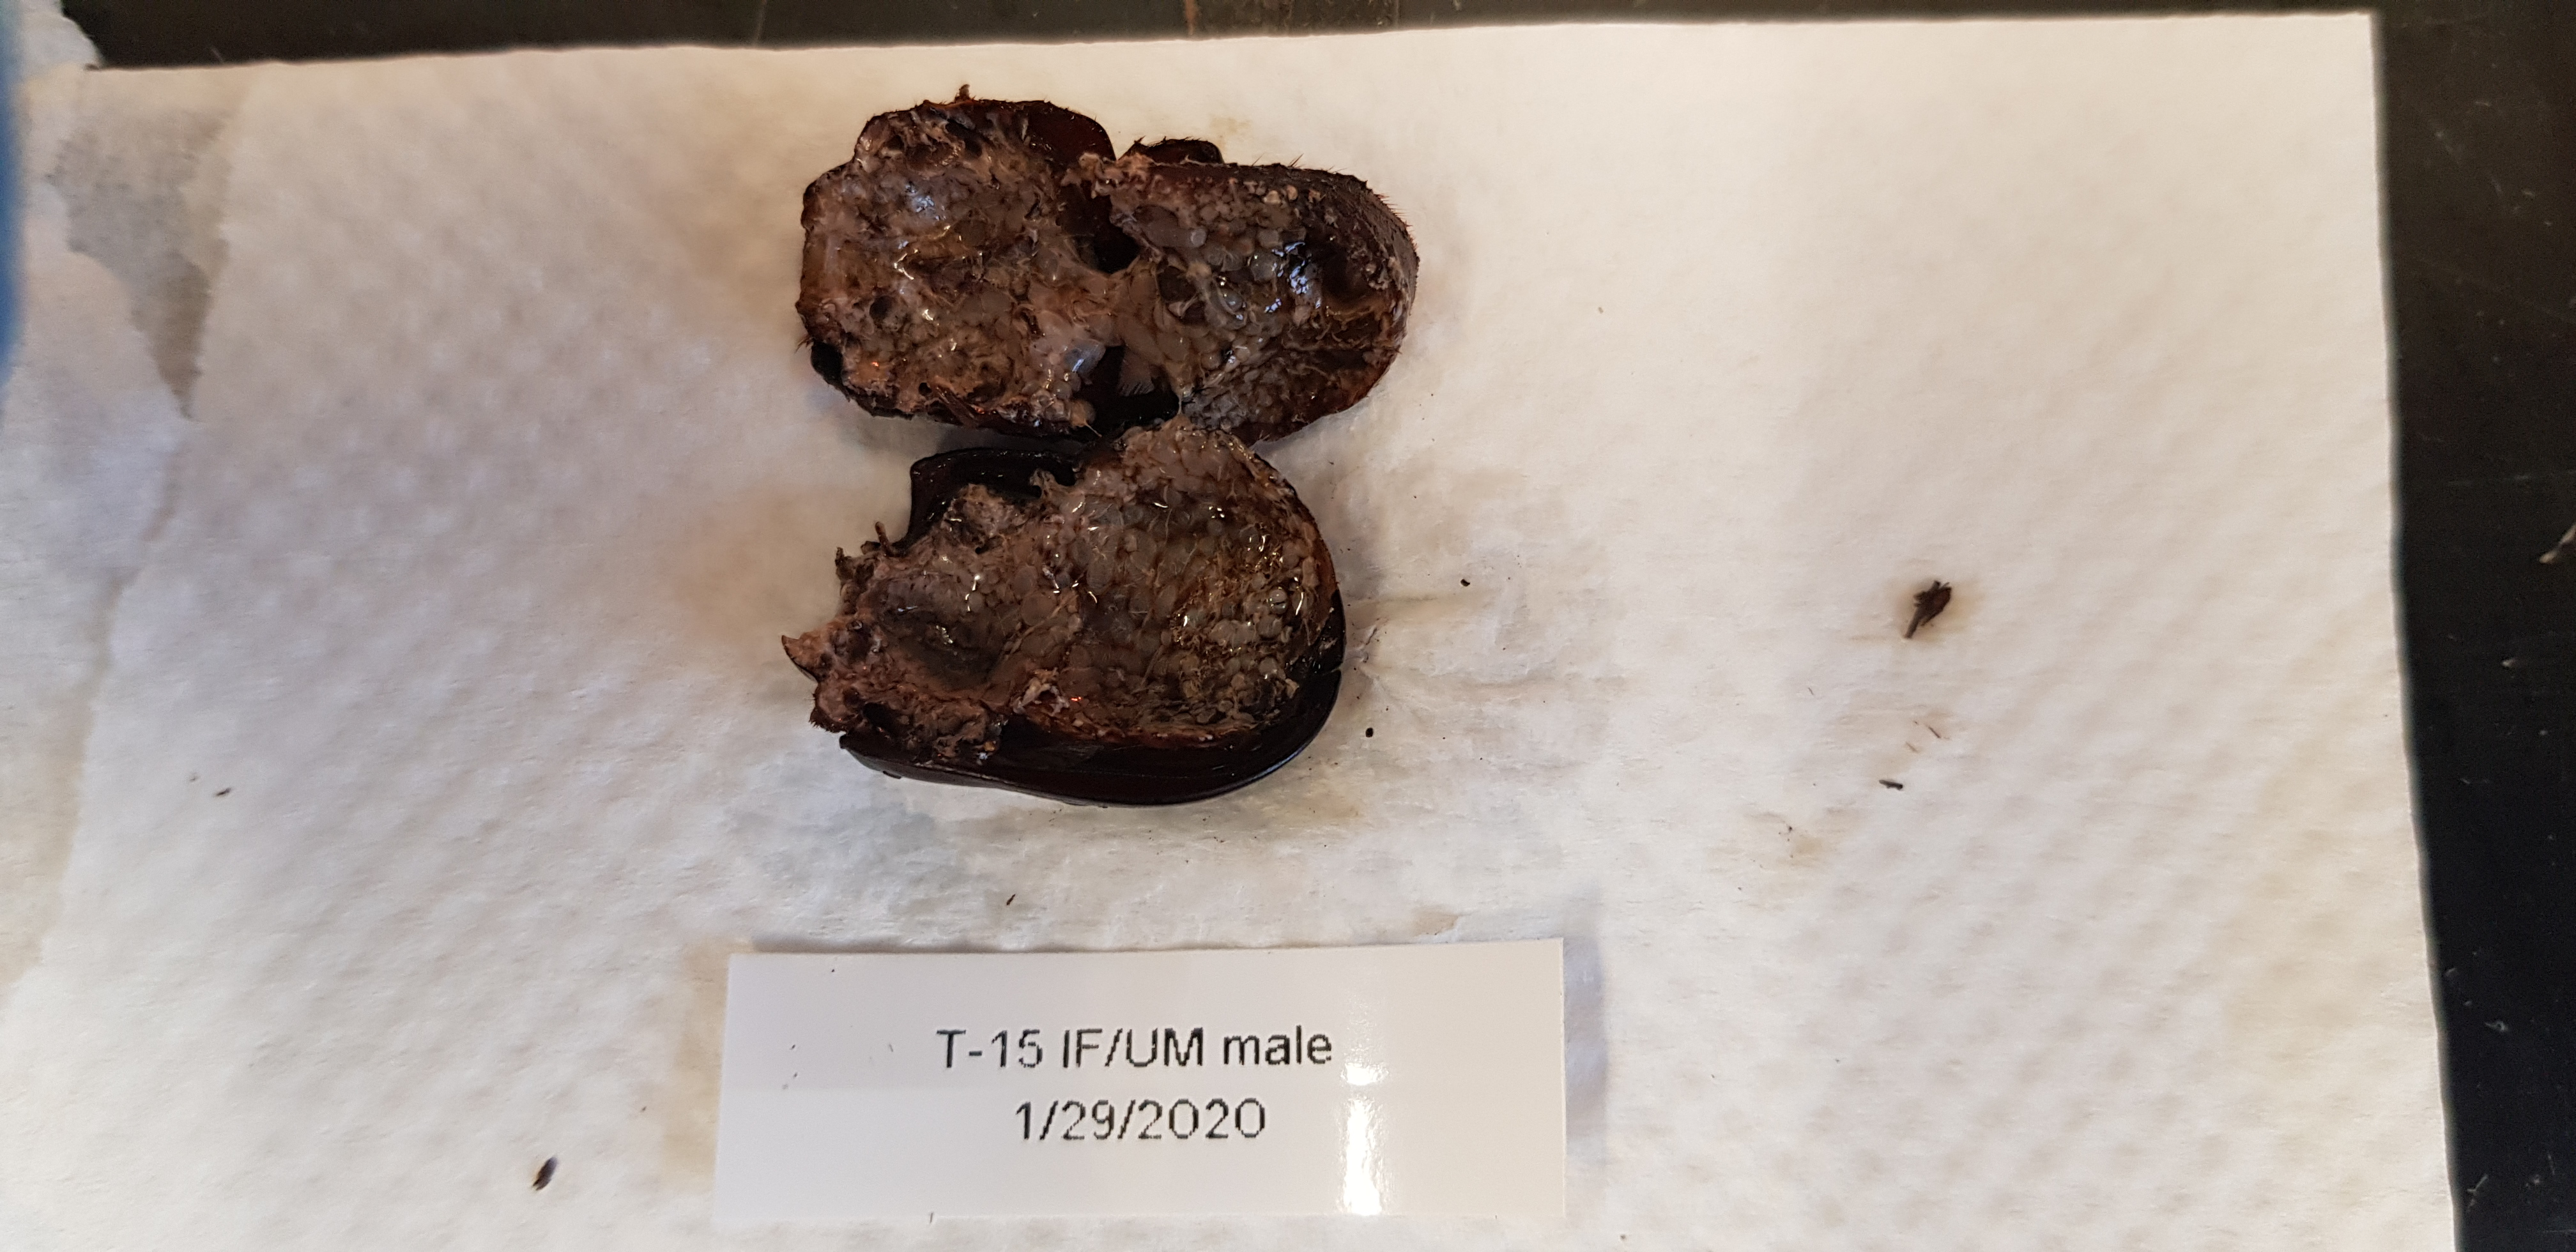
\includegraphics[width=\textwidth]{pm-images/20200129_153950.jpg}
\caption{\textbf{TF15m} jar\_id                                TF15
sex                                      m
treatment                        companion
date\_treated           2019-12-27 00:00:00
date\_died              2020-01-29 00:00:00
postmortem\_virus                       NaN
postmortem\_bacteria                      1
pm\_image\_filename      20200129\_153950.jpg
date\_end\_bioassay      2020-02-06 00:00:00
t                                       33
e                                     True
Name: 44, dtype: object}
\end{figure}
\clearpage

\begin{figure}[h!]
\centering
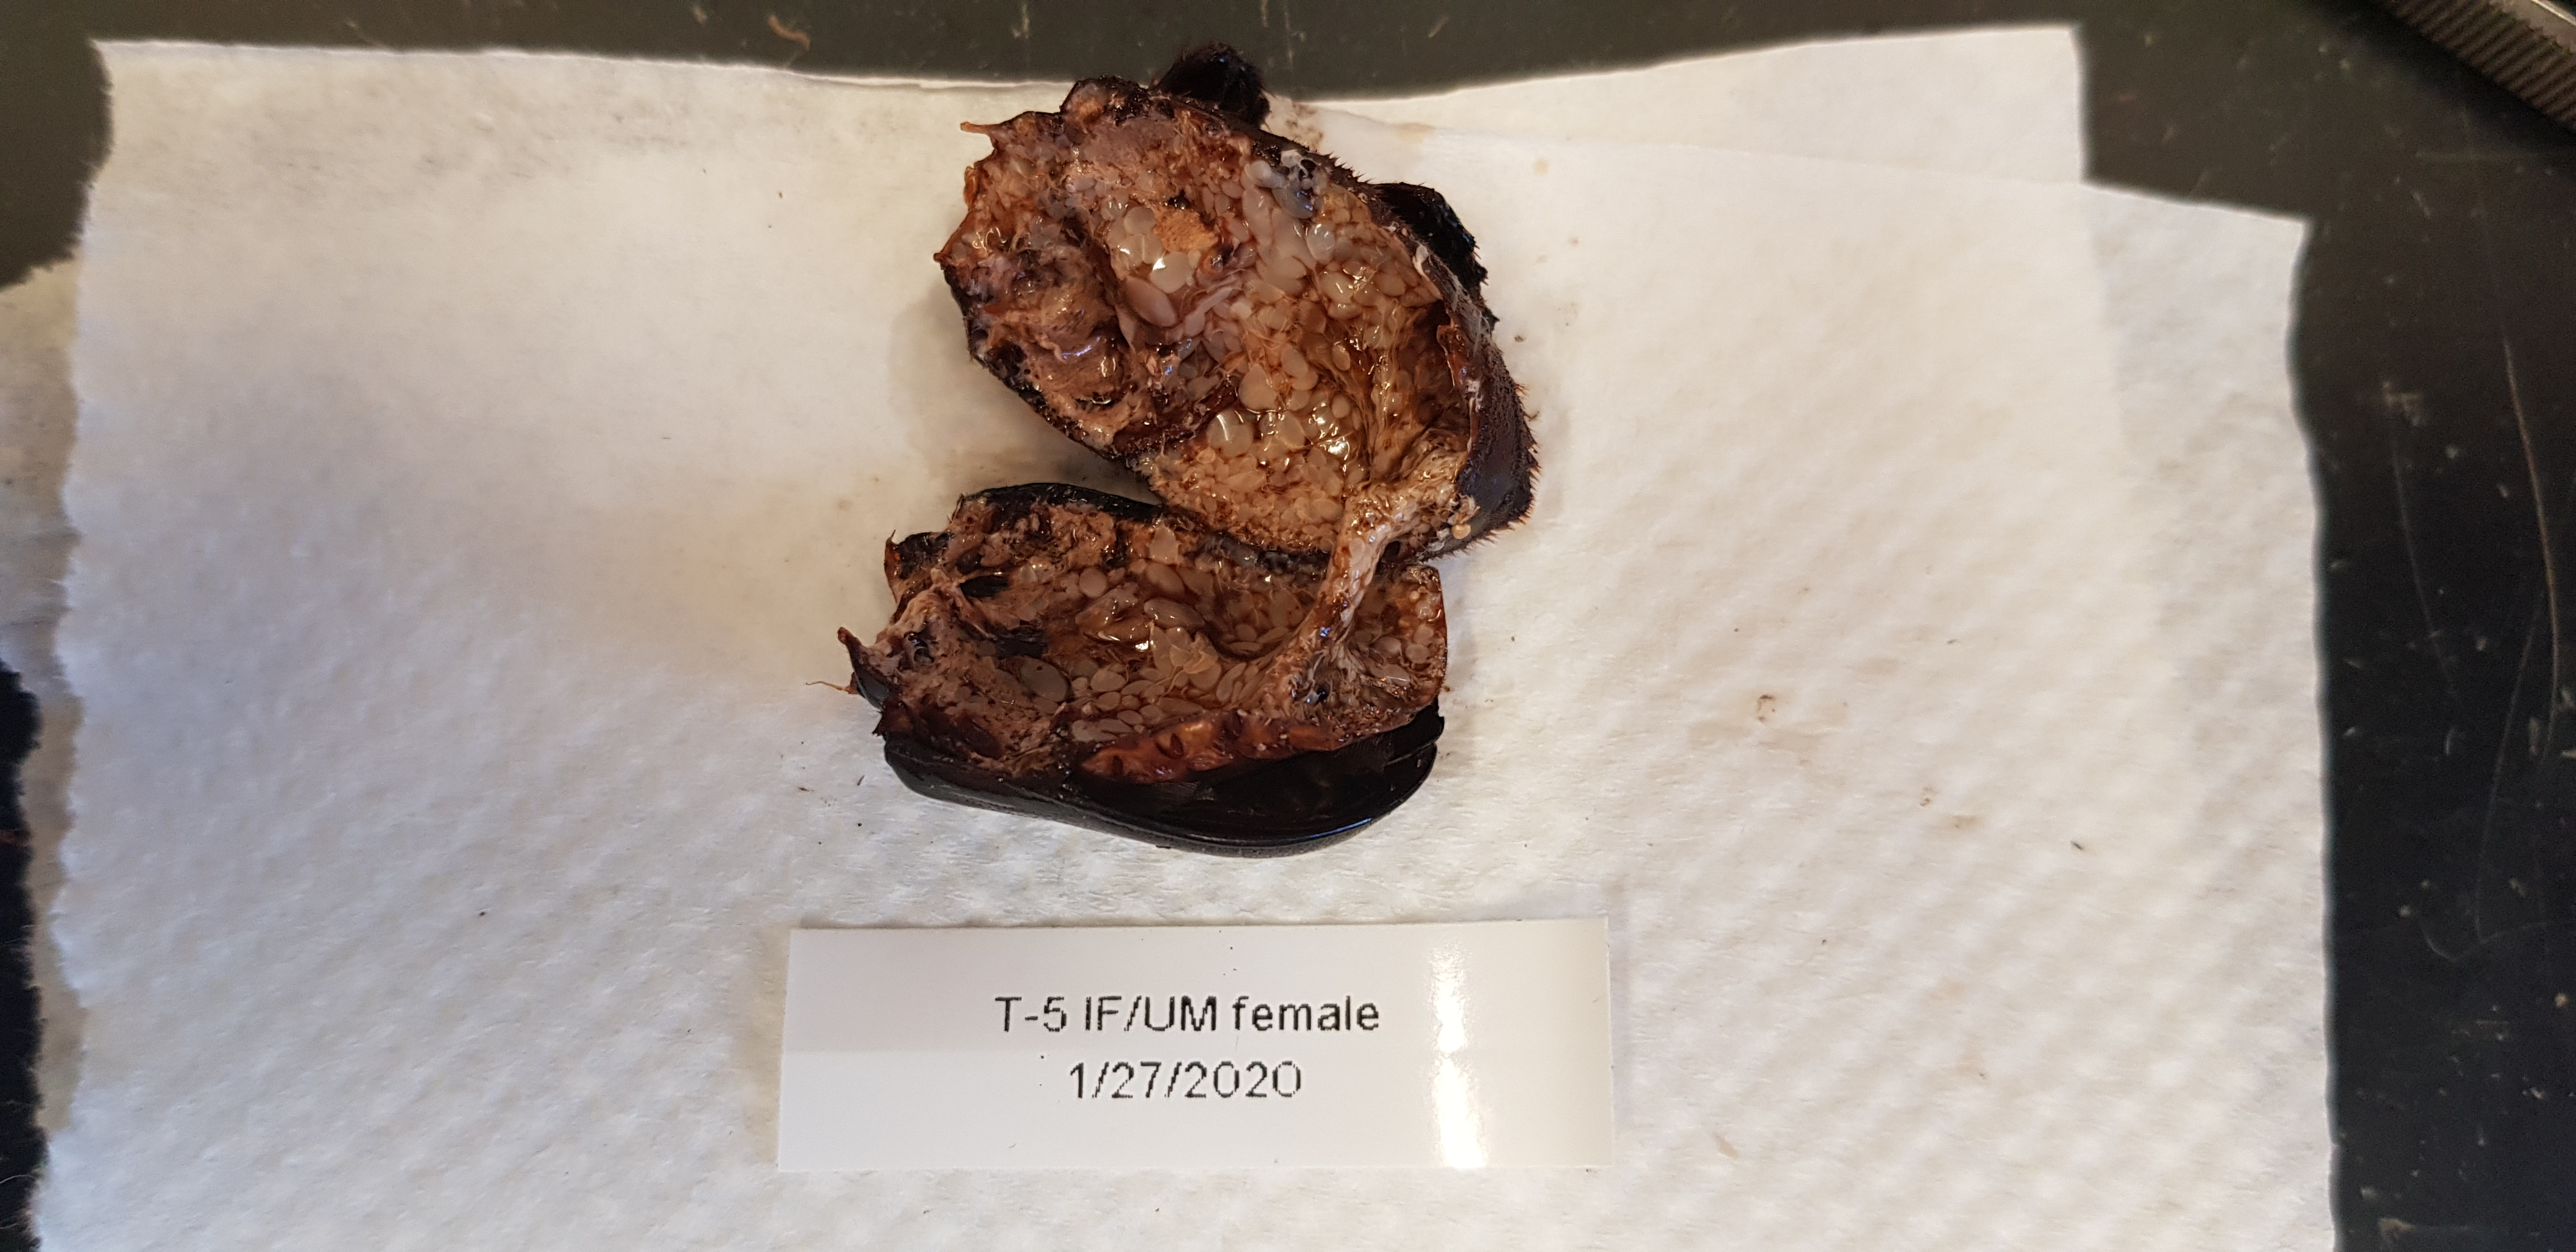
\includegraphics[width=\textwidth]{pm-images/20200127_151015.jpg}
\caption{\textbf{TF2f} jar\_id                                 TF2
sex                                      f
treatment                            virus
date\_treated           2019-12-26 00:00:00
date\_died                              NaT
postmortem\_virus                       NaN
postmortem\_bacteria                    NaN
pm\_image\_filename      20200127\_151015.jpg
date\_end\_bioassay      2020-02-06 00:00:00
t                                       42
e                                    False
Name: 46, dtype: object}
\end{figure}
\clearpage

\begin{figure}[h!]
\centering
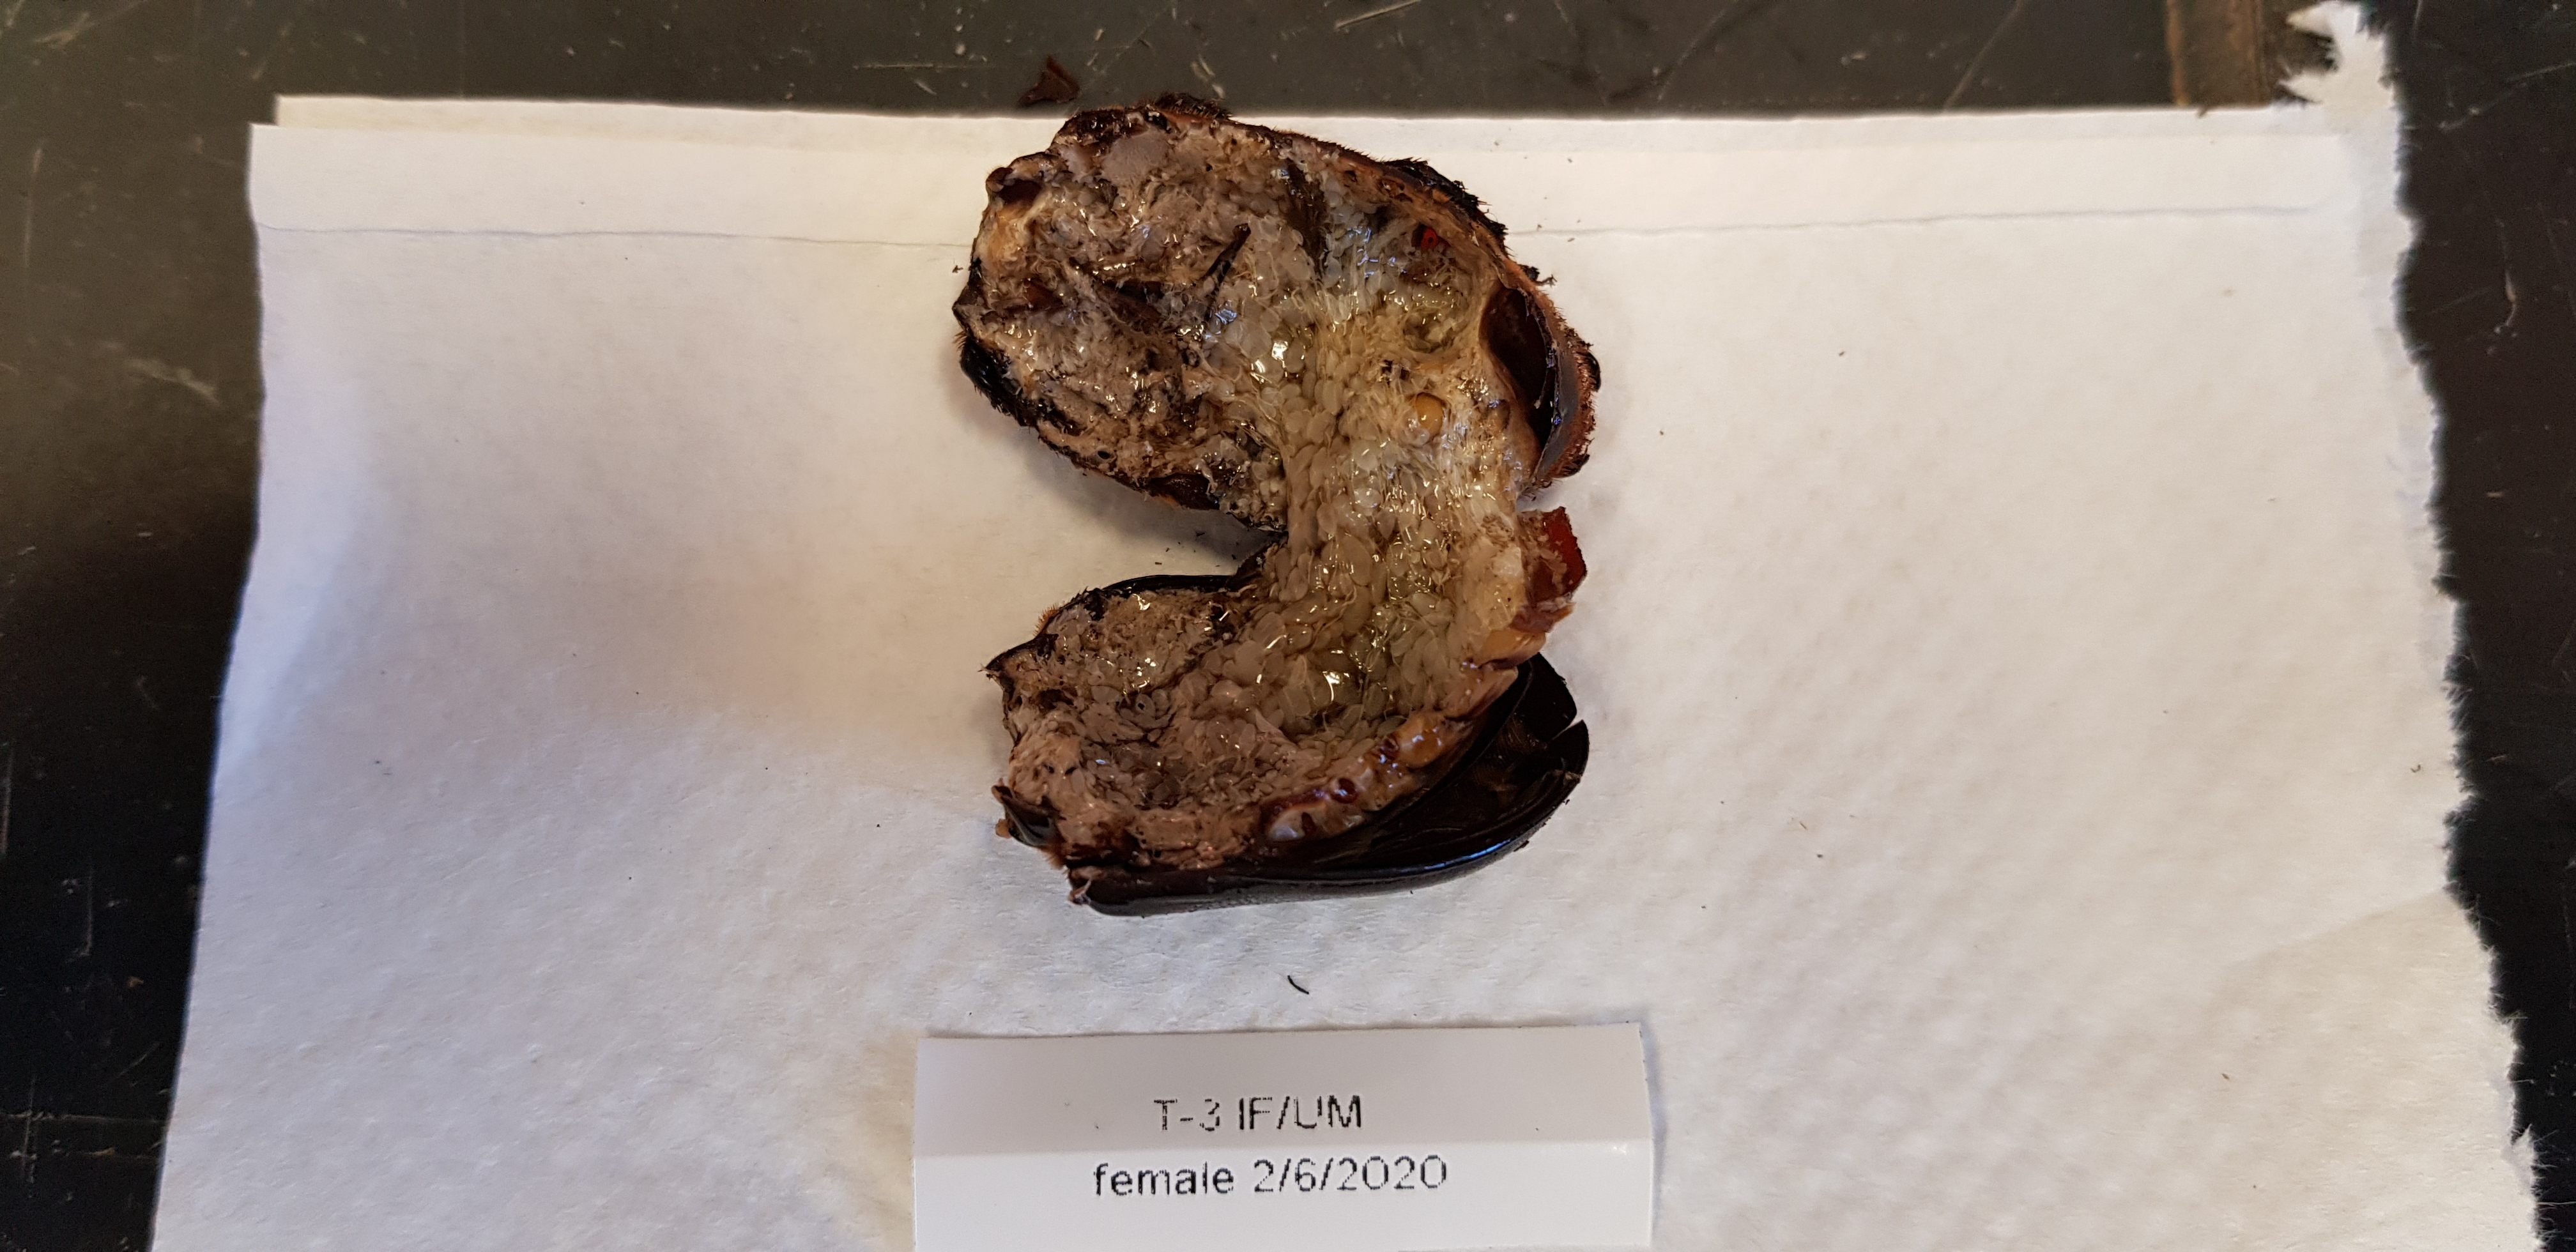
\includegraphics[width=\textwidth]{pm-images/20200206_113817.jpg}
\caption{\textbf{TF3f} jar\_id                                 TF3
sex                                      f
treatment                            virus
date\_treated           2019-12-26 00:00:00
date\_died              2020-02-06 00:00:00
postmortem\_virus                       NaN
postmortem\_bacteria                    NaN
pm\_image\_filename      20200206\_113817.jpg
date\_end\_bioassay      2020-02-06 00:00:00
t                                       42
e                                     True
Name: 47, dtype: object}
\end{figure}
\clearpage

\begin{figure}[h!]
\centering
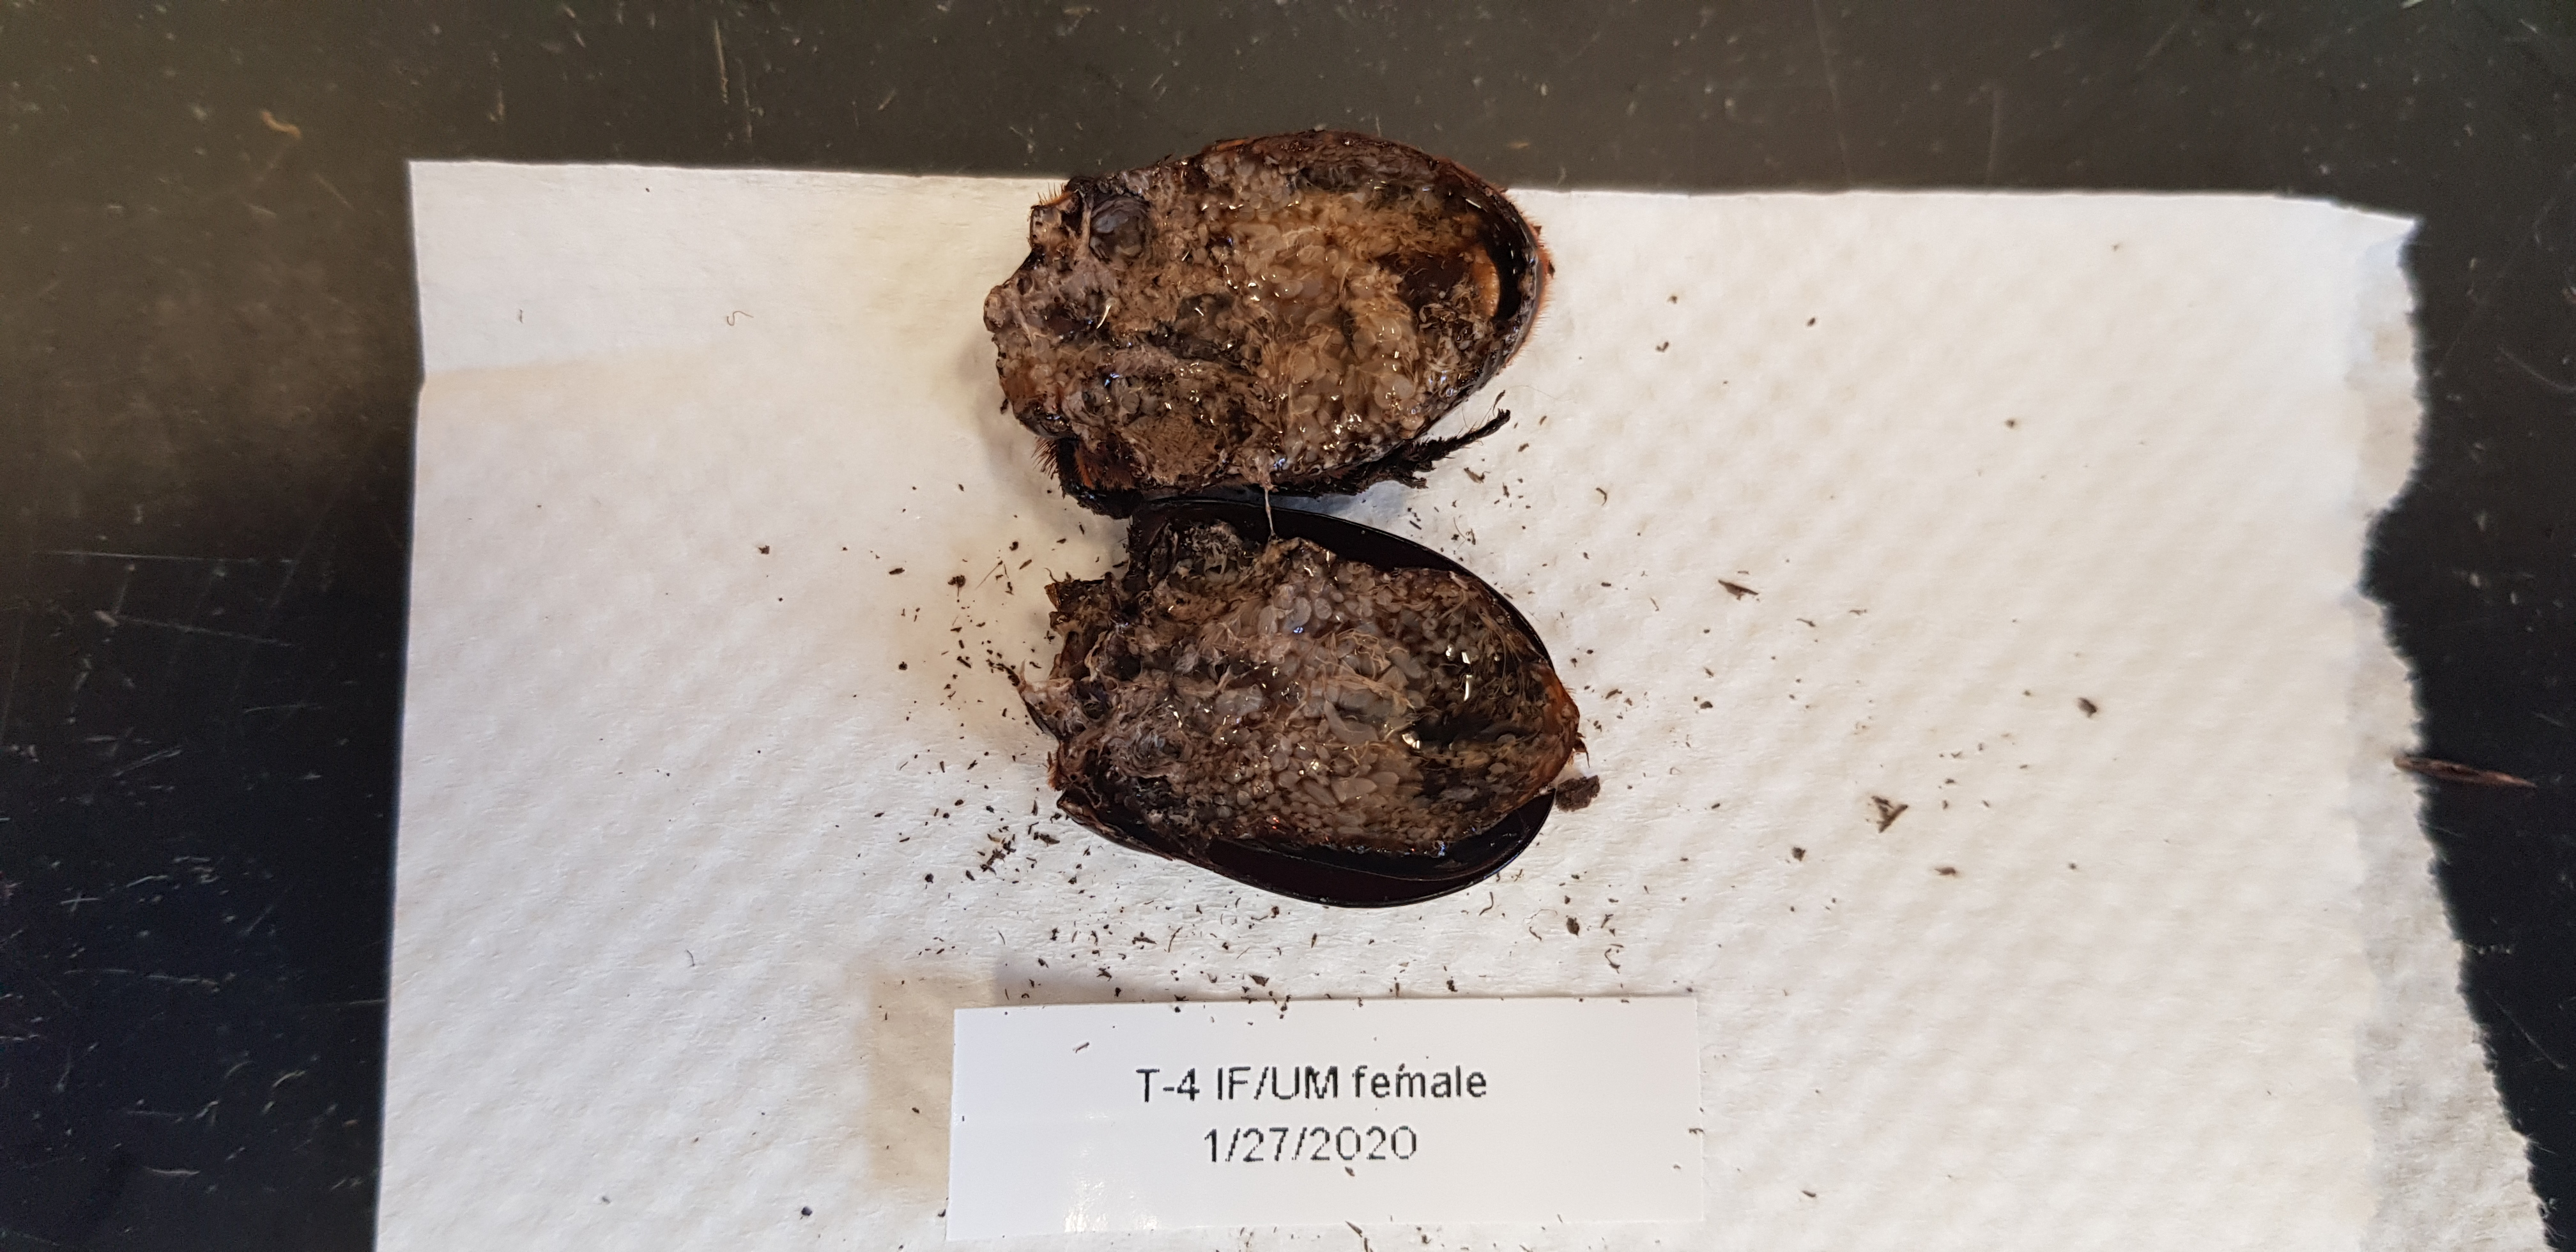
\includegraphics[width=\textwidth]{pm-images/20200127_145553.jpg}
\caption{\textbf{TF4f} jar\_id                                 TF4
sex                                      f
treatment                            virus
date\_treated           2019-12-26 00:00:00
date\_died              2020-01-27 00:00:00
postmortem\_virus                       NaN
postmortem\_bacteria                    NaN
pm\_image\_filename      20200127\_145553.jpg
date\_end\_bioassay      2020-02-06 00:00:00
t                                       32
e                                     True
Name: 48, dtype: object}
\end{figure}
\clearpage

\begin{figure}[h!]
\centering
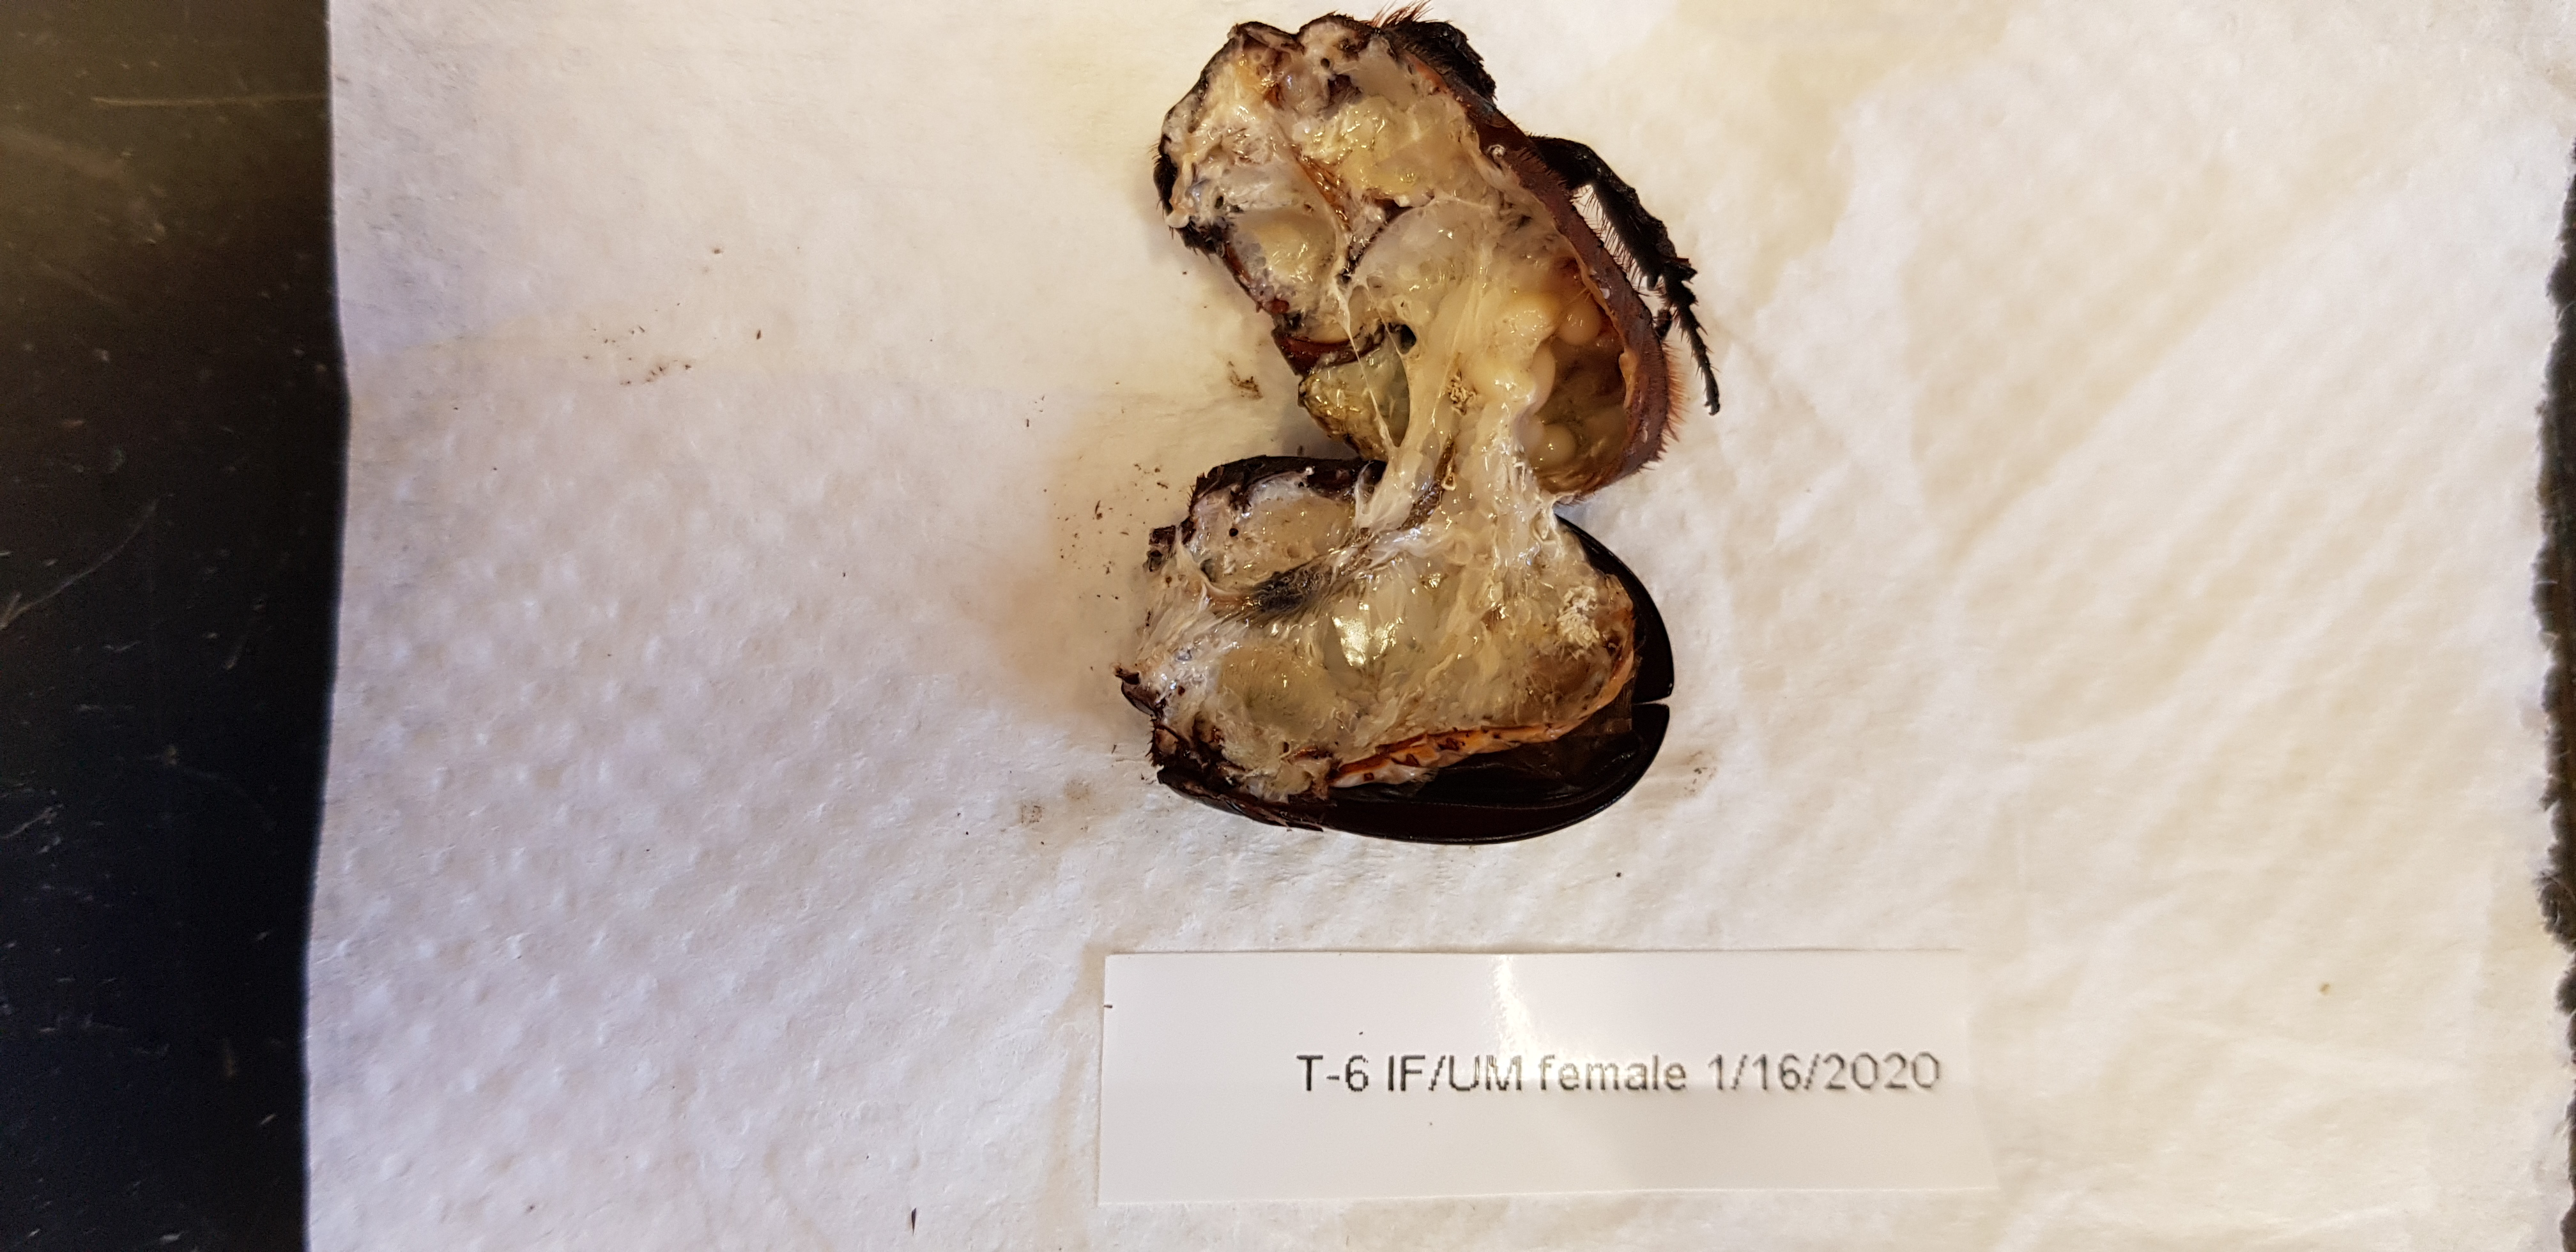
\includegraphics[width=\textwidth]{pm-images/20200116_112000.jpg}
\caption{\textbf{TF6f} jar\_id                                 TF6
sex                                      f
treatment                            virus
date\_treated           2019-12-27 00:00:00
date\_died              2020-01-16 00:00:00
postmortem\_virus                       NaN
postmortem\_bacteria                      1
pm\_image\_filename      20200116\_112000.jpg
date\_end\_bioassay      2020-02-06 00:00:00
t                                       20
e                                     True
Name: 50, dtype: object}
\end{figure}
\clearpage

\begin{figure}[h!]
\centering
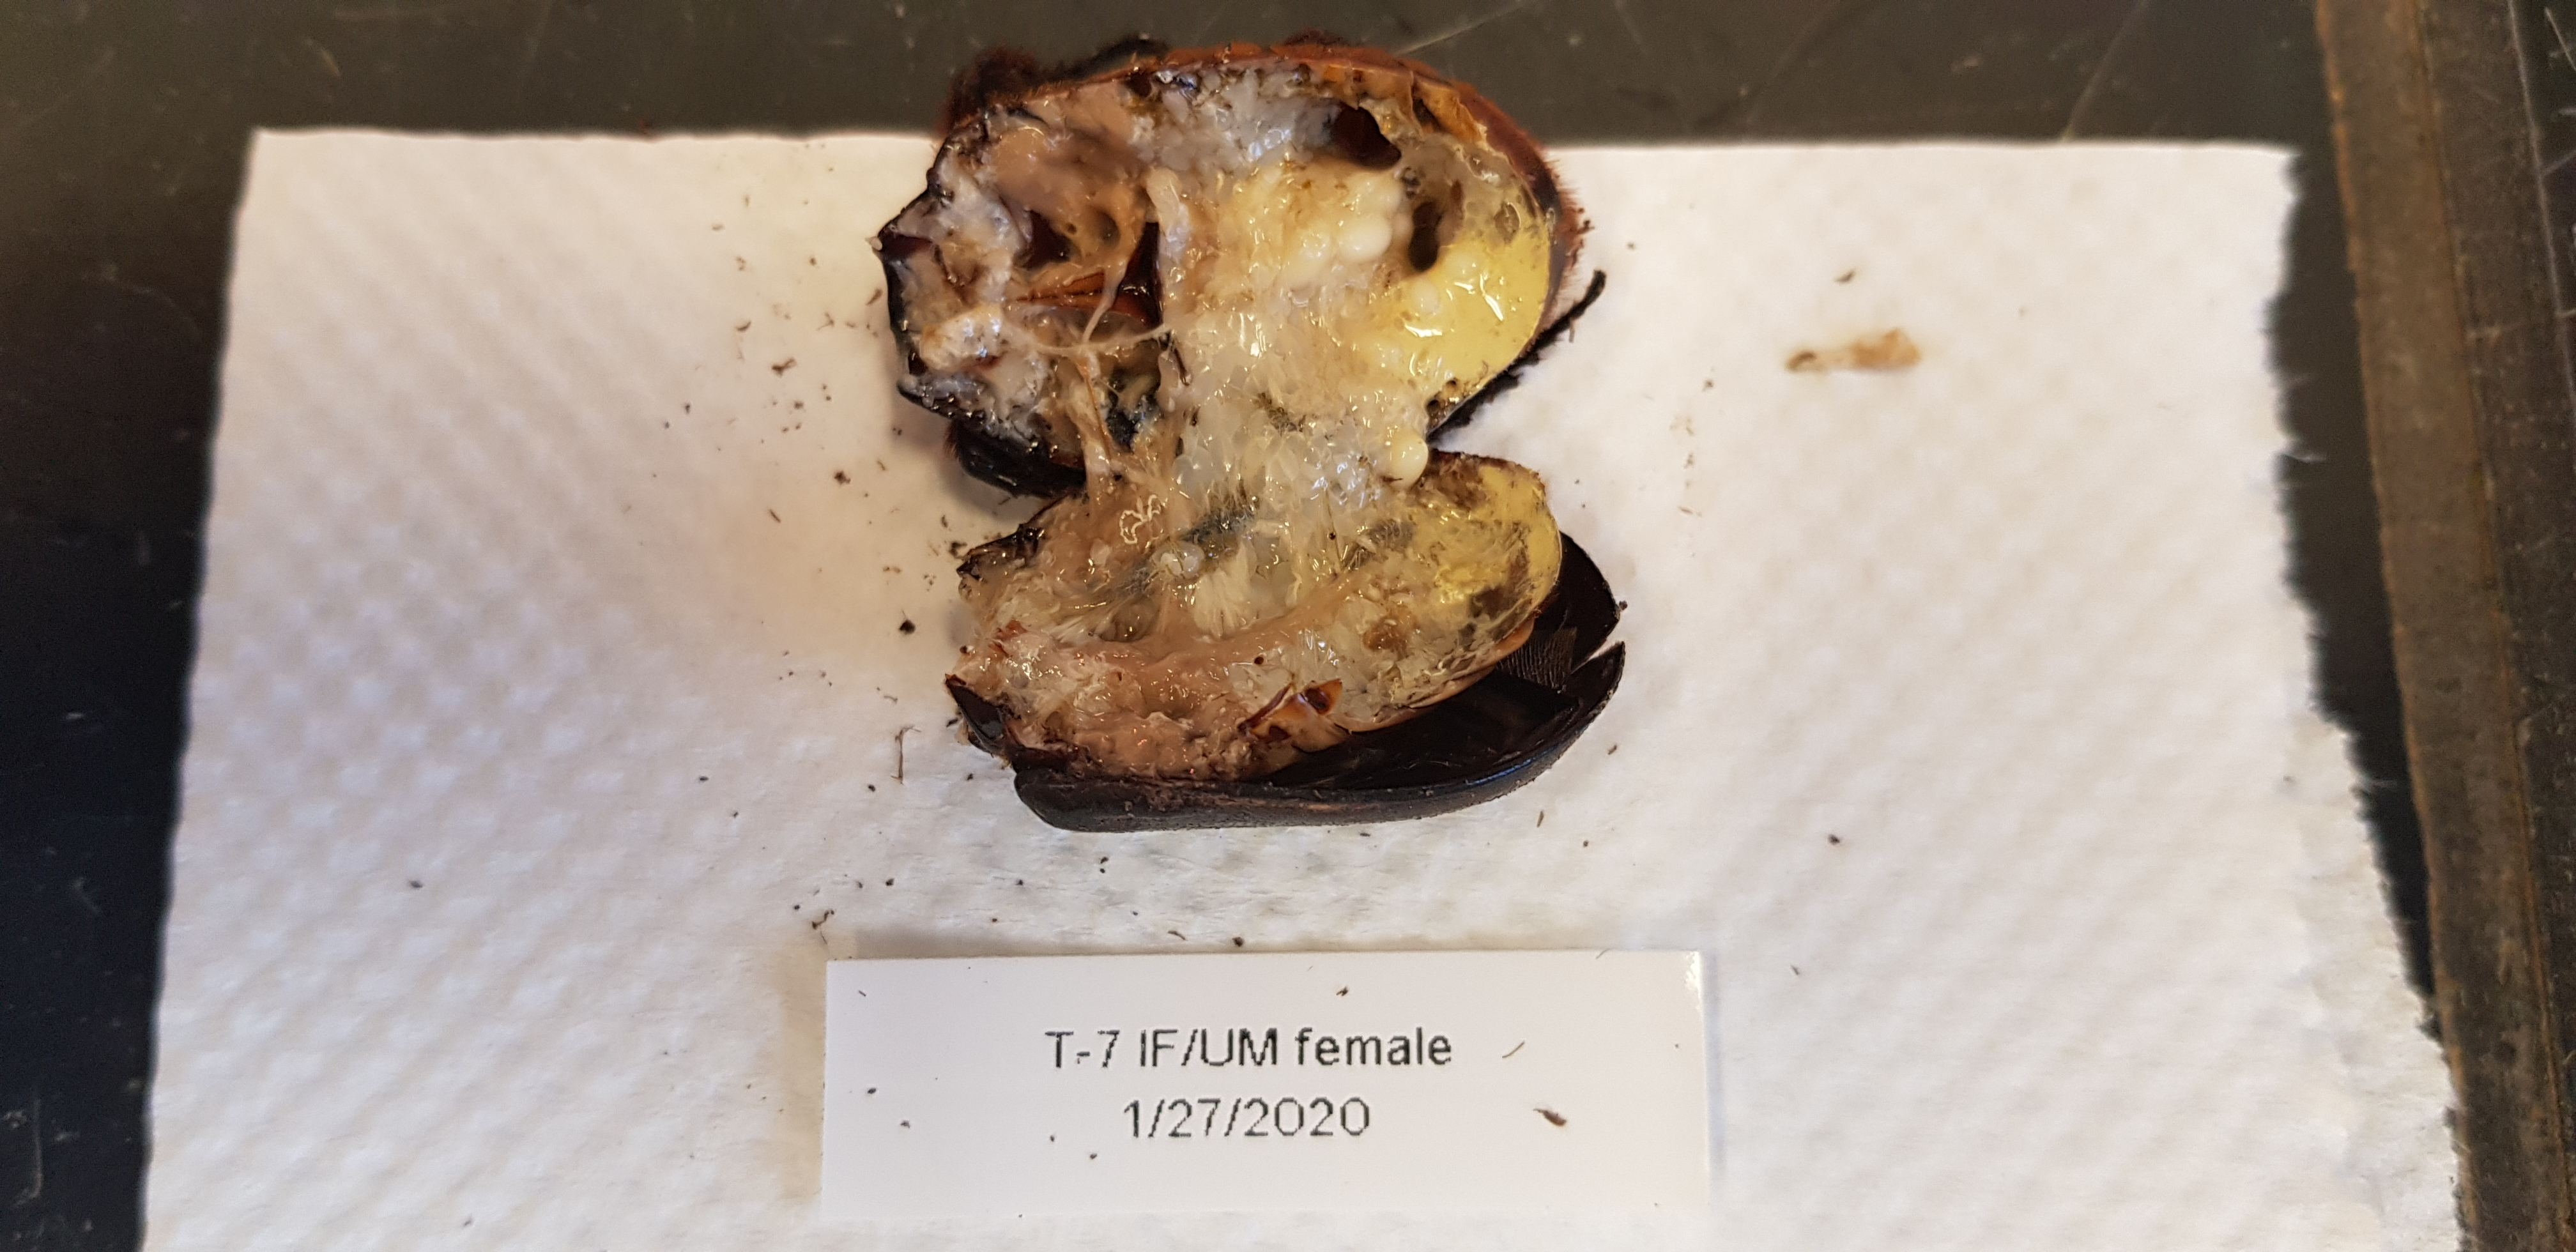
\includegraphics[width=\textwidth]{pm-images/20200127_144326.jpg}
\caption{\textbf{TF7f} jar\_id                                 TF7
sex                                      f
treatment                            virus
date\_treated           2019-12-27 00:00:00
date\_died              2020-01-27 00:00:00
postmortem\_virus                       NaN
postmortem\_bacteria                      1
pm\_image\_filename      20200127\_144326.jpg
date\_end\_bioassay      2020-02-06 00:00:00
t                                       31
e                                     True
Name: 51, dtype: object}
\end{figure}
\clearpage

\begin{figure}[h!]
\centering
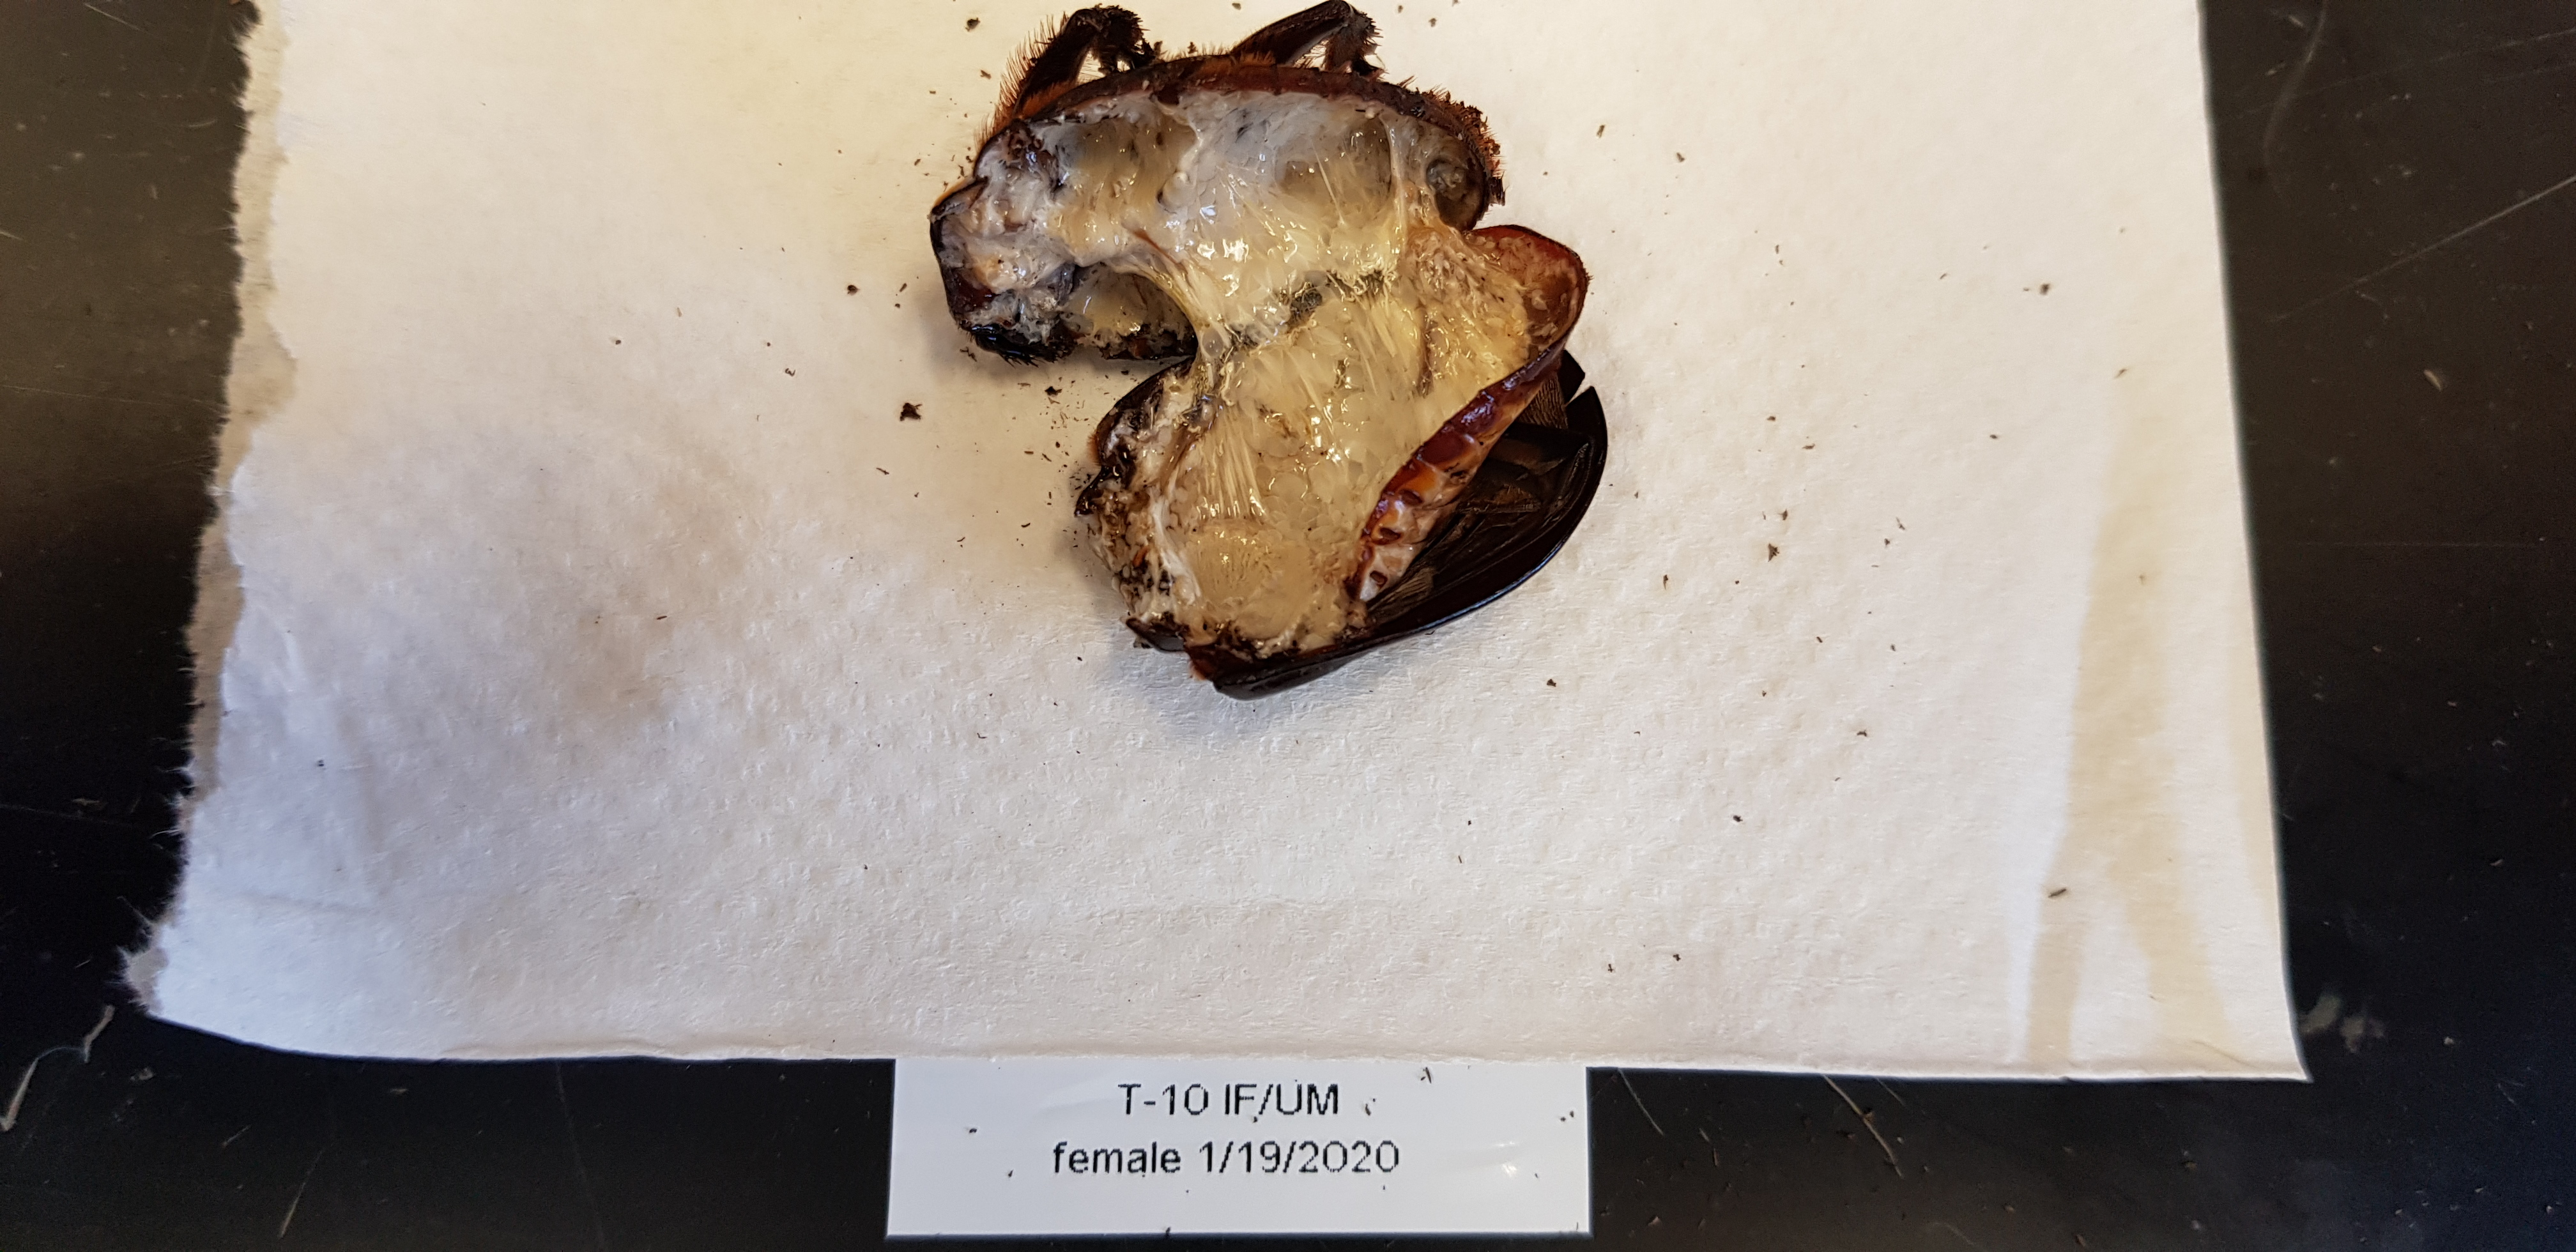
\includegraphics[width=\textwidth]{pm-images/20200119_123529.jpg}
\caption{\textbf{TF10f} jar\_id                                TF10
sex                                      f
treatment                            virus
date\_treated           2019-12-27 00:00:00
date\_died              2020-01-19 00:00:00
postmortem\_virus                       NaN
postmortem\_bacteria                    NaN
pm\_image\_filename      20200119\_123529.jpg
date\_end\_bioassay      2020-02-06 00:00:00
t                                       23
e                                     True
Name: 54, dtype: object}
\end{figure}
\clearpage

\begin{figure}[h!]
\centering
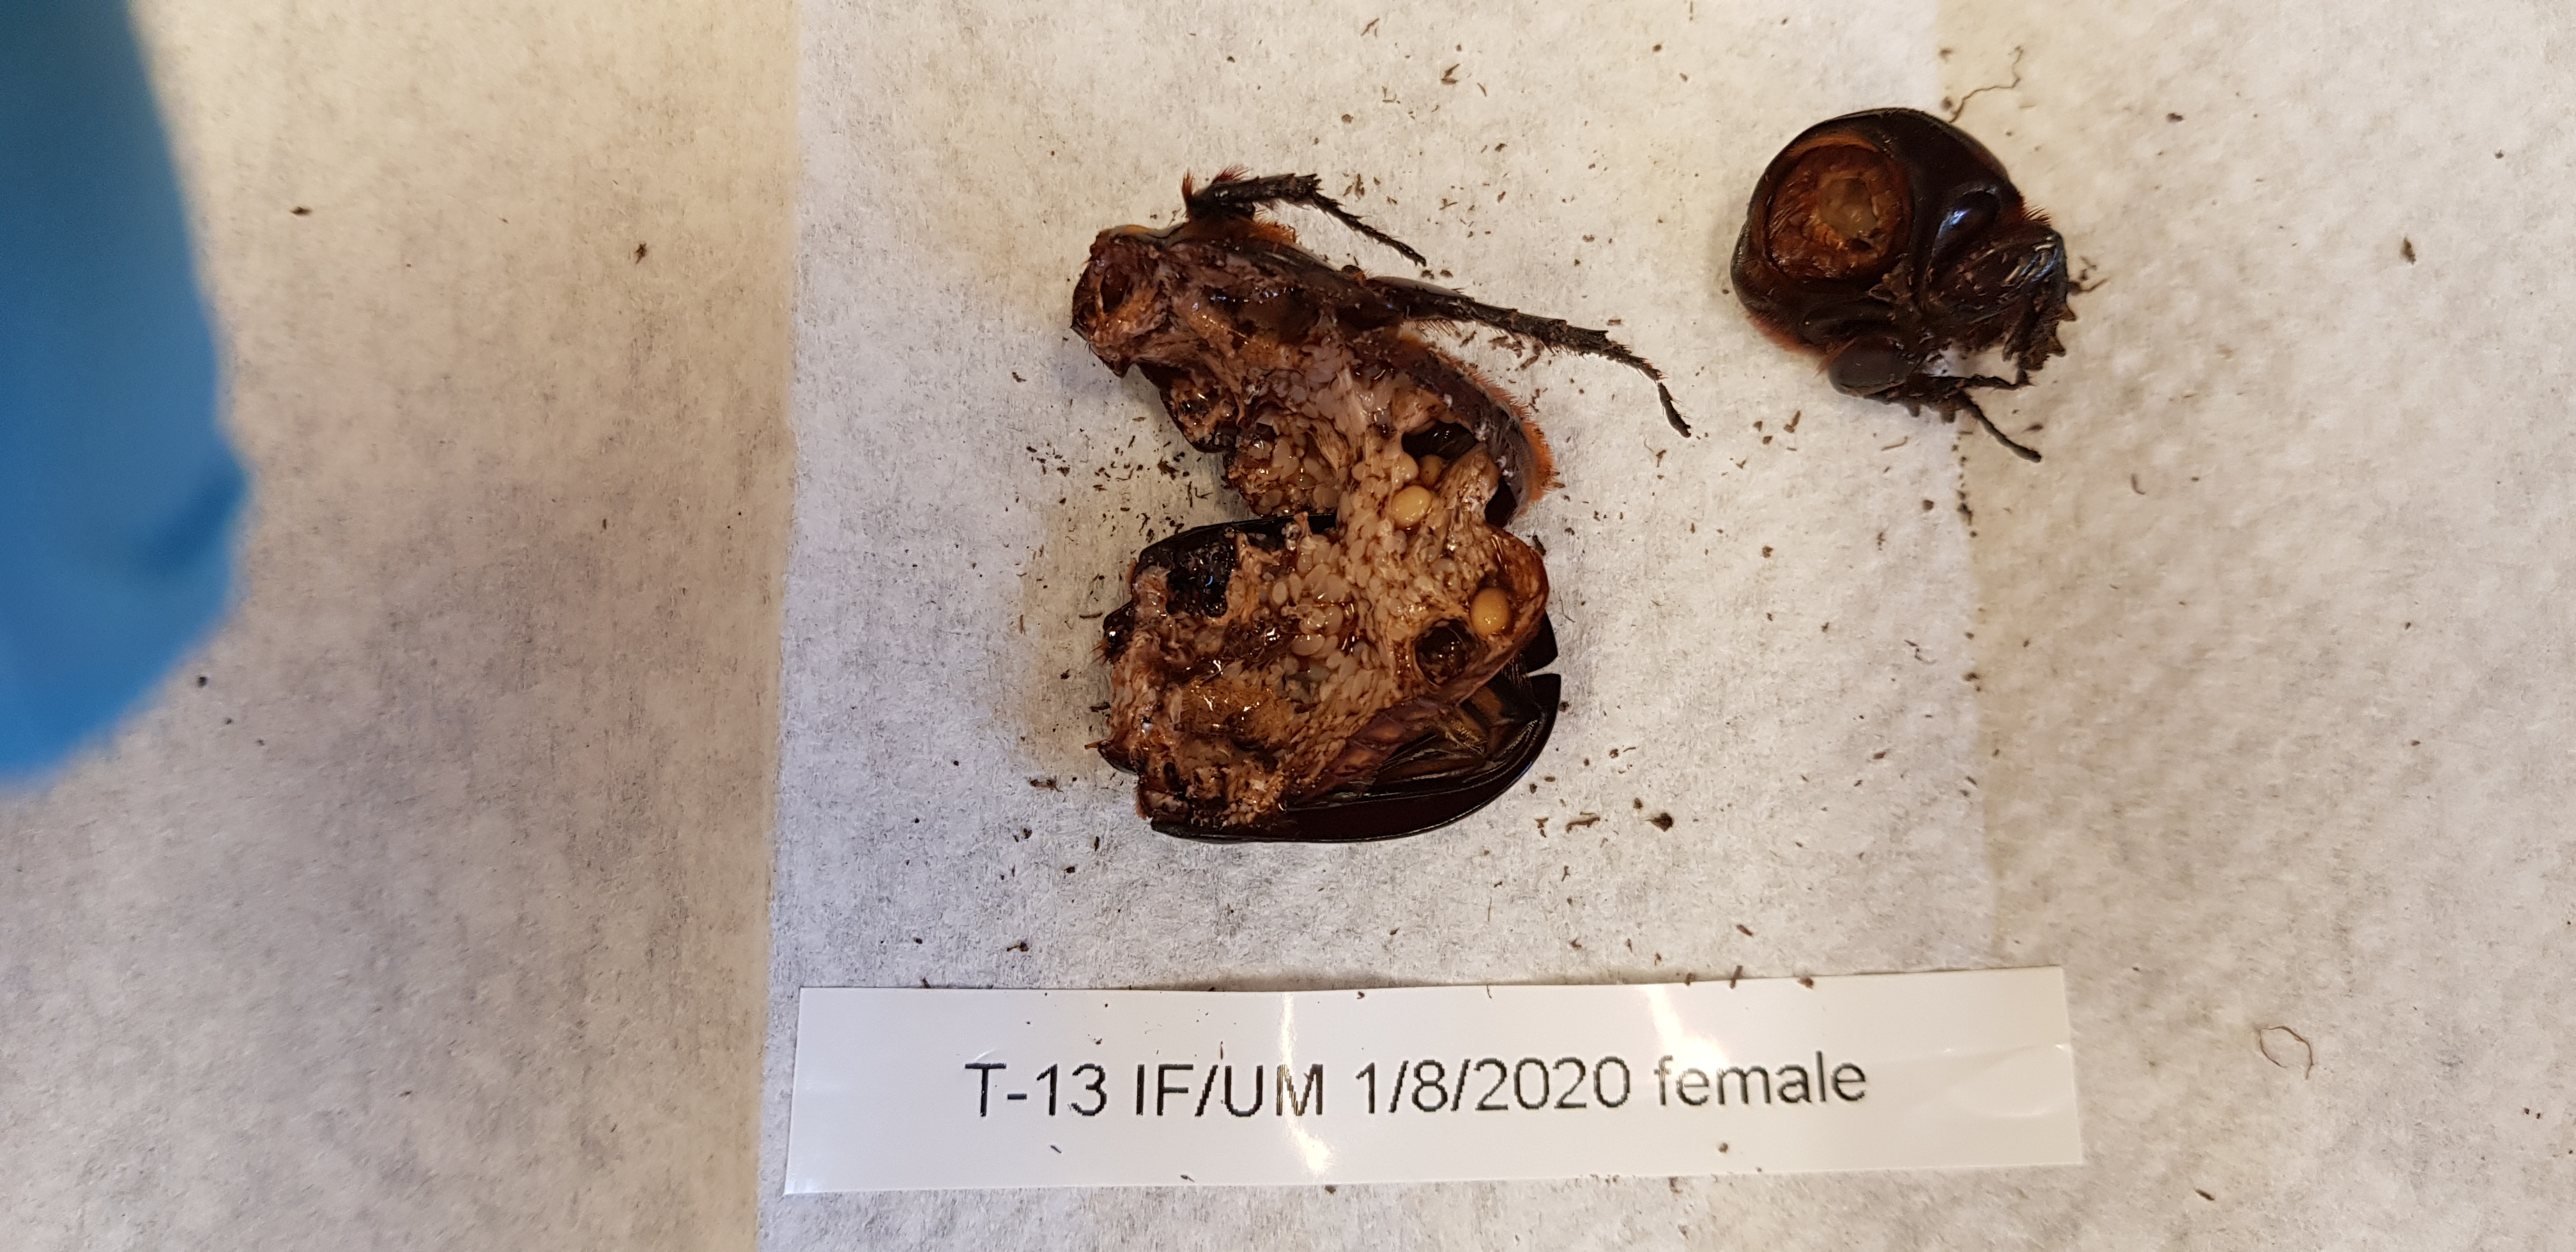
\includegraphics[width=\textwidth]{pm-images/20200108_101434.jpg}
\caption{\textbf{TF13f} jar\_id                                TF13
sex                                      f
treatment                            virus
date\_treated           2019-12-27 00:00:00
date\_died              2020-01-08 00:00:00
postmortem\_virus                       NaN
postmortem\_bacteria                      1
pm\_image\_filename      20200108\_101434.jpg
date\_end\_bioassay      2020-02-06 00:00:00
t                                       12
e                                     True
Name: 57, dtype: object}
\end{figure}
\clearpage

\begin{figure}[h!]
\centering
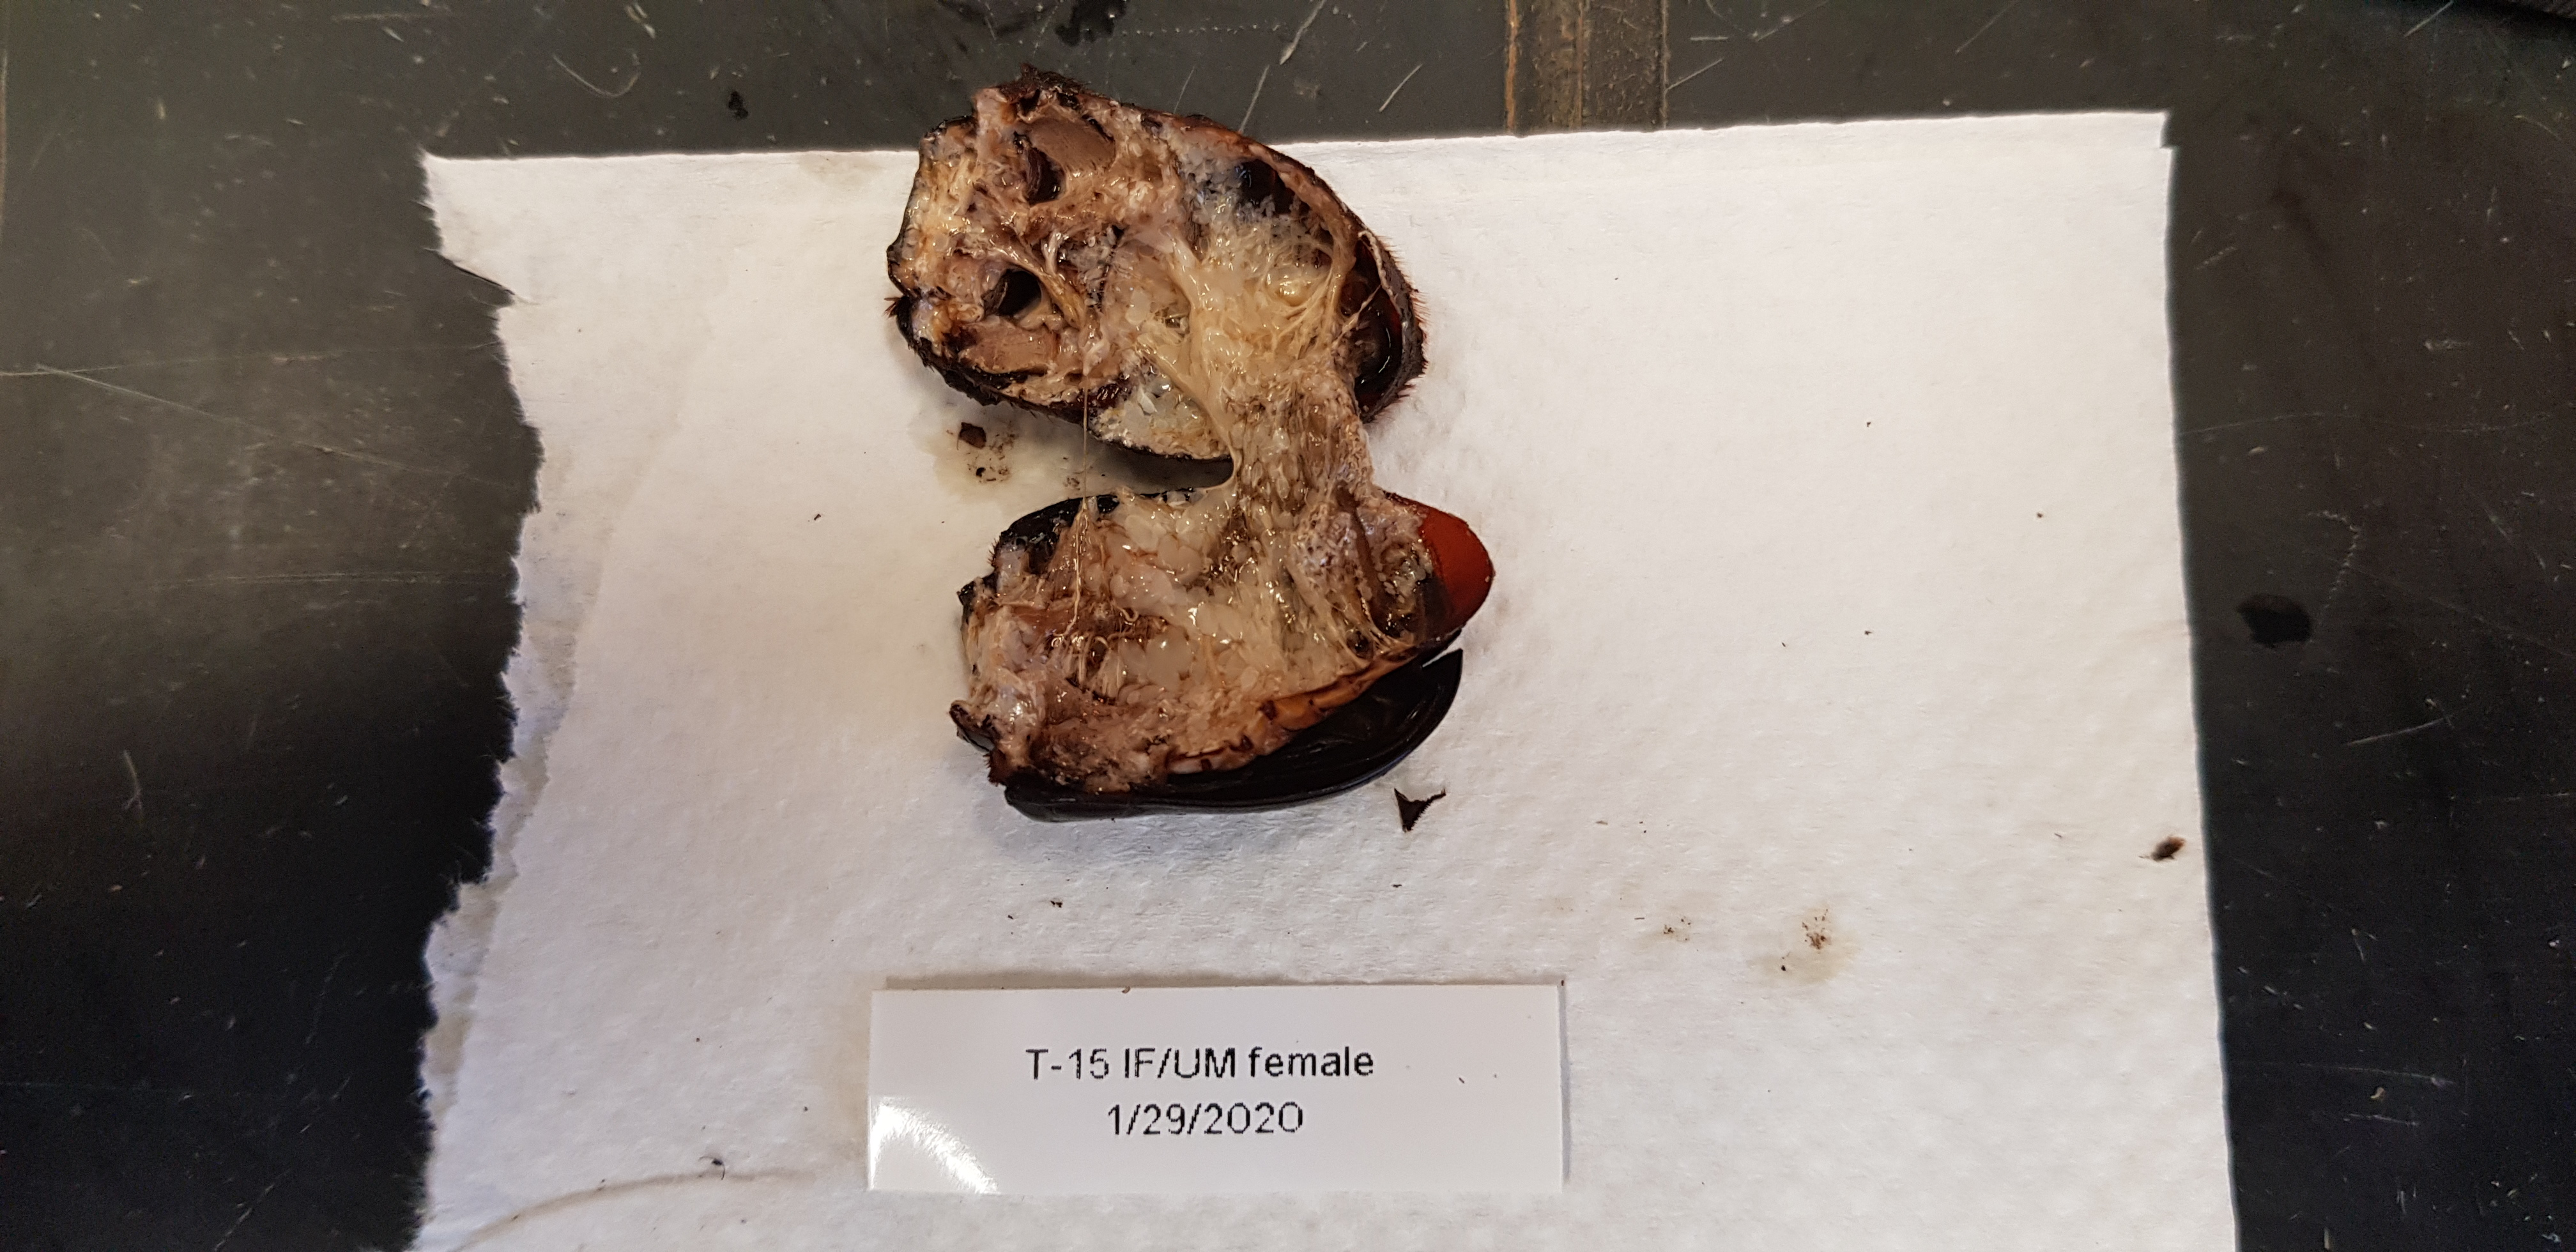
\includegraphics[width=\textwidth]{pm-images/20200129_153605.jpg}
\caption{\textbf{TF15f} jar\_id                                TF15
sex                                      f
treatment                            virus
date\_treated           2019-12-27 00:00:00
date\_died              2020-01-29 00:00:00
postmortem\_virus                       NaN
postmortem\_bacteria                      1
pm\_image\_filename      20200129\_153605.jpg
date\_end\_bioassay      2020-02-06 00:00:00
t                                       33
e                                     True
Name: 59, dtype: object}
\end{figure}
\clearpage

\begin{figure}[h!]
\centering
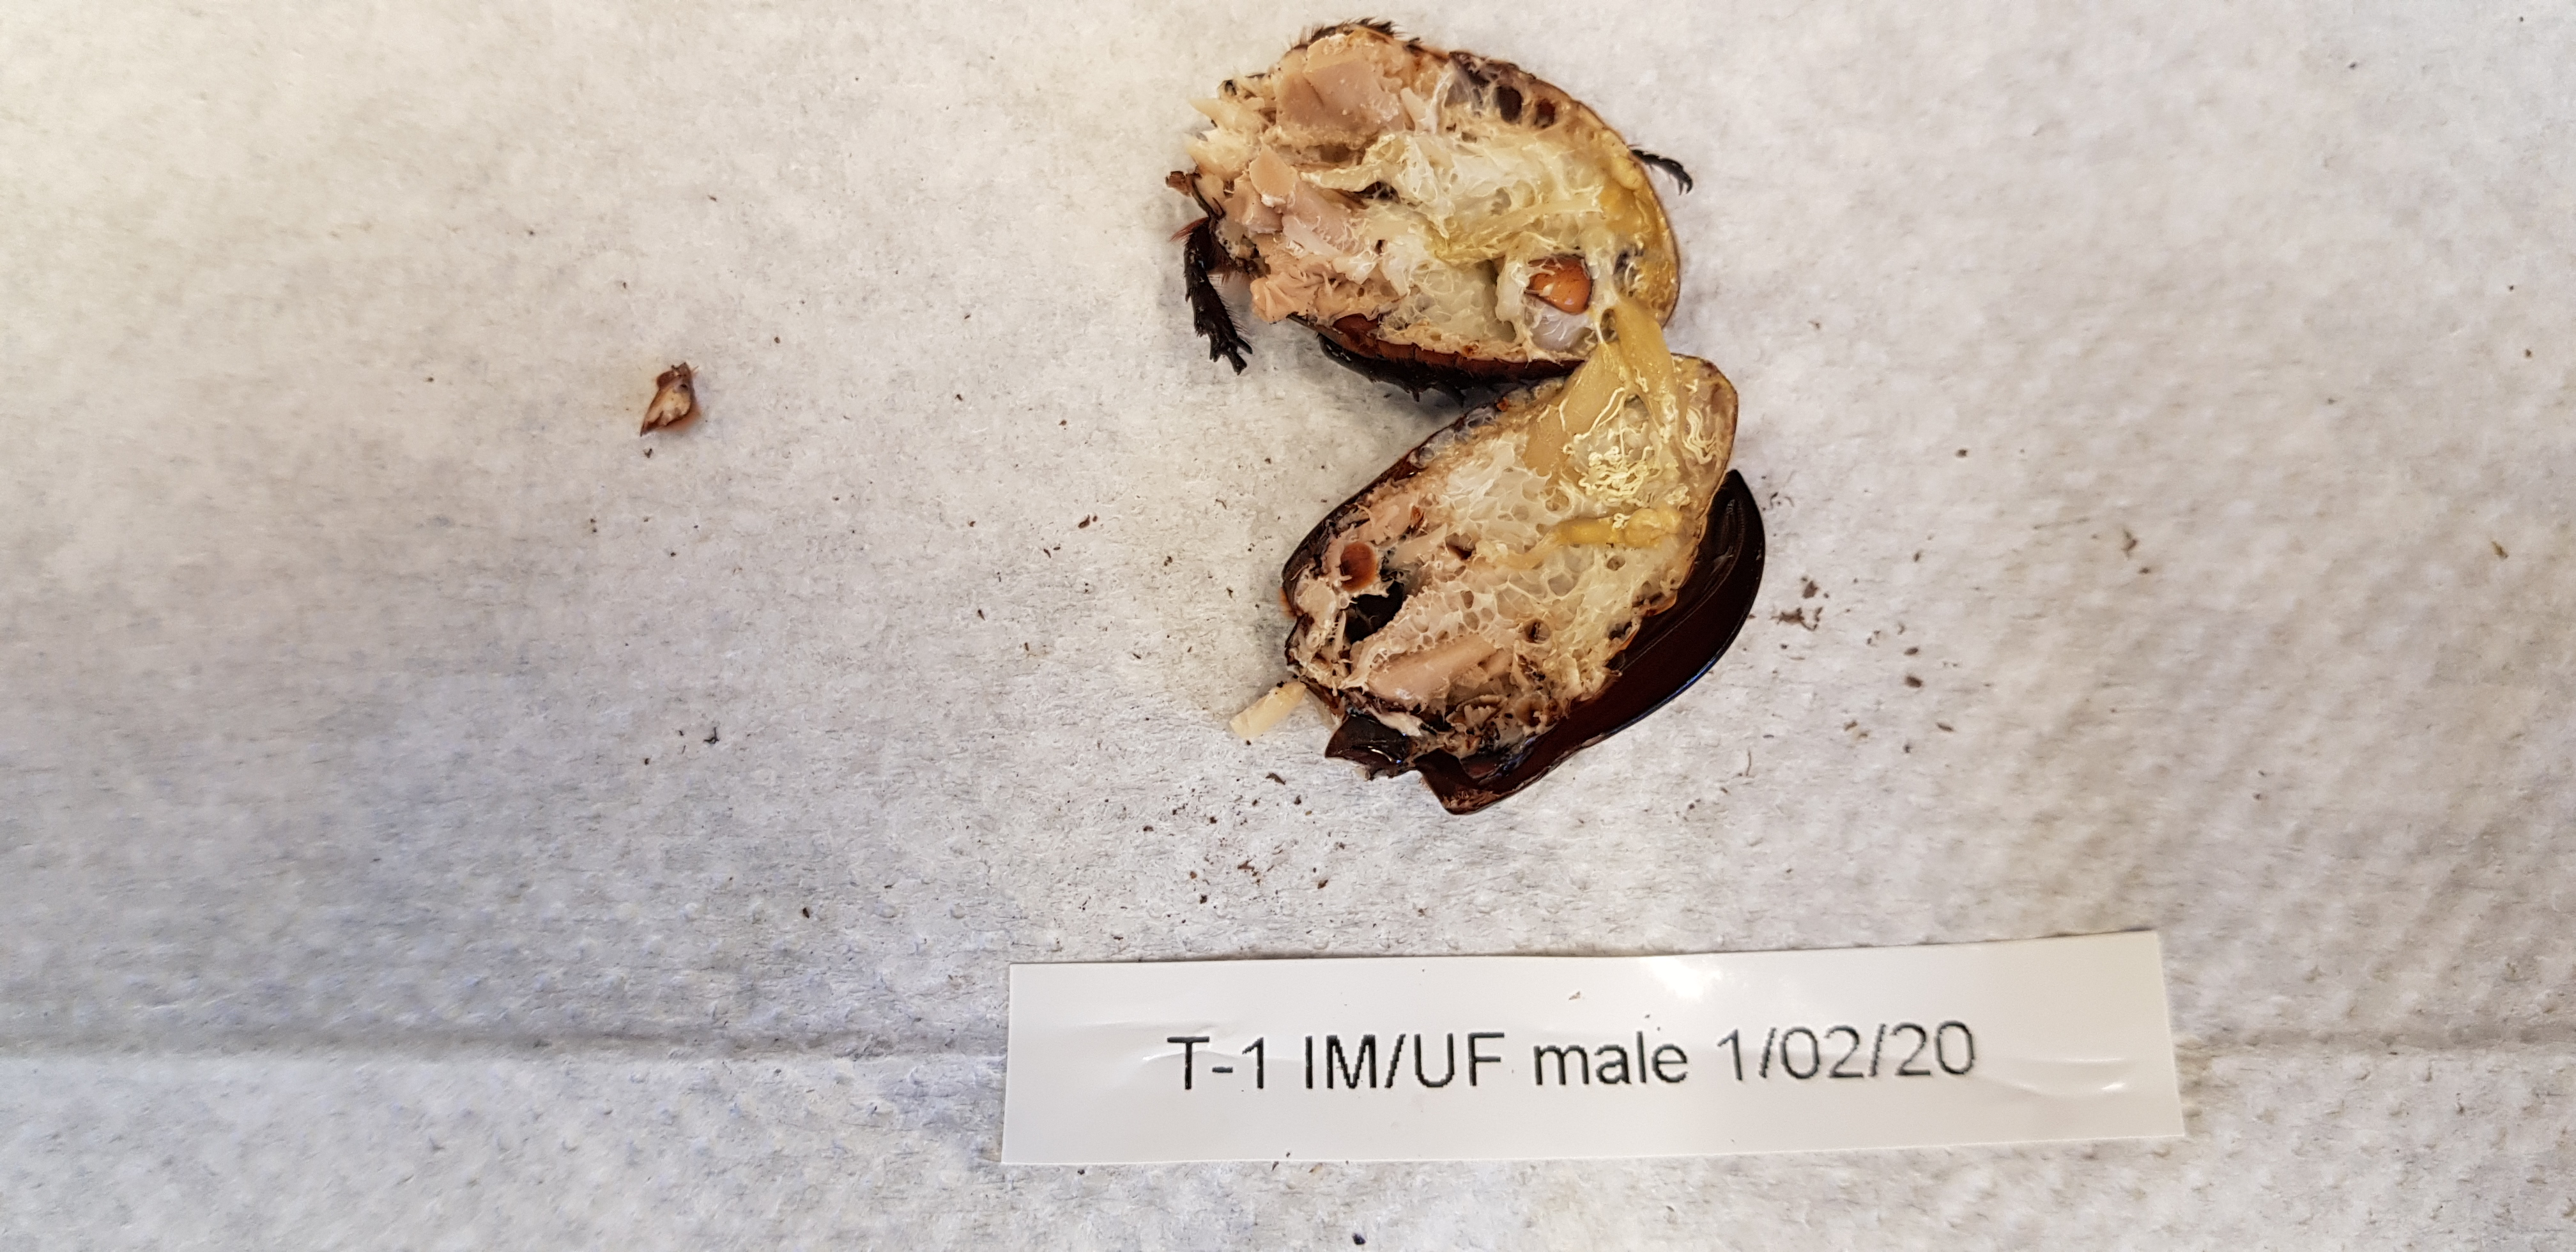
\includegraphics[width=\textwidth]{pm-images/20200102_111008.jpg}
\caption{\textbf{TM1m} jar\_id                                 TM1
sex                                      m
treatment                            virus
date\_treated           2019-12-26 00:00:00
date\_died              2020-01-02 00:00:00
postmortem\_virus                       NaN
postmortem\_bacteria                    NaN
pm\_image\_filename      20200102\_111008.jpg
date\_end\_bioassay      2020-02-06 00:00:00
t                                        7
e                                     True
Name: 60, dtype: object}
\end{figure}
\clearpage

\begin{figure}[h!]
\centering
\includegraphics[width=\textwidth]{pm-images/20200211_114845_001.jpg}
\caption{\textbf{TM2m} jar\_id                                     TM2
sex                                          m
treatment                                virus
date\_treated               2019-12-26 00:00:00
date\_died                                  NaT
postmortem\_virus                           NaN
postmortem\_bacteria                        NaN
pm\_image\_filename      20200211\_114845\_001.jpg
date\_end\_bioassay          2020-02-06 00:00:00
t                                           42
e                                        False
Name: 61, dtype: object}
\end{figure}
\clearpage

\begin{figure}[h!]
\centering
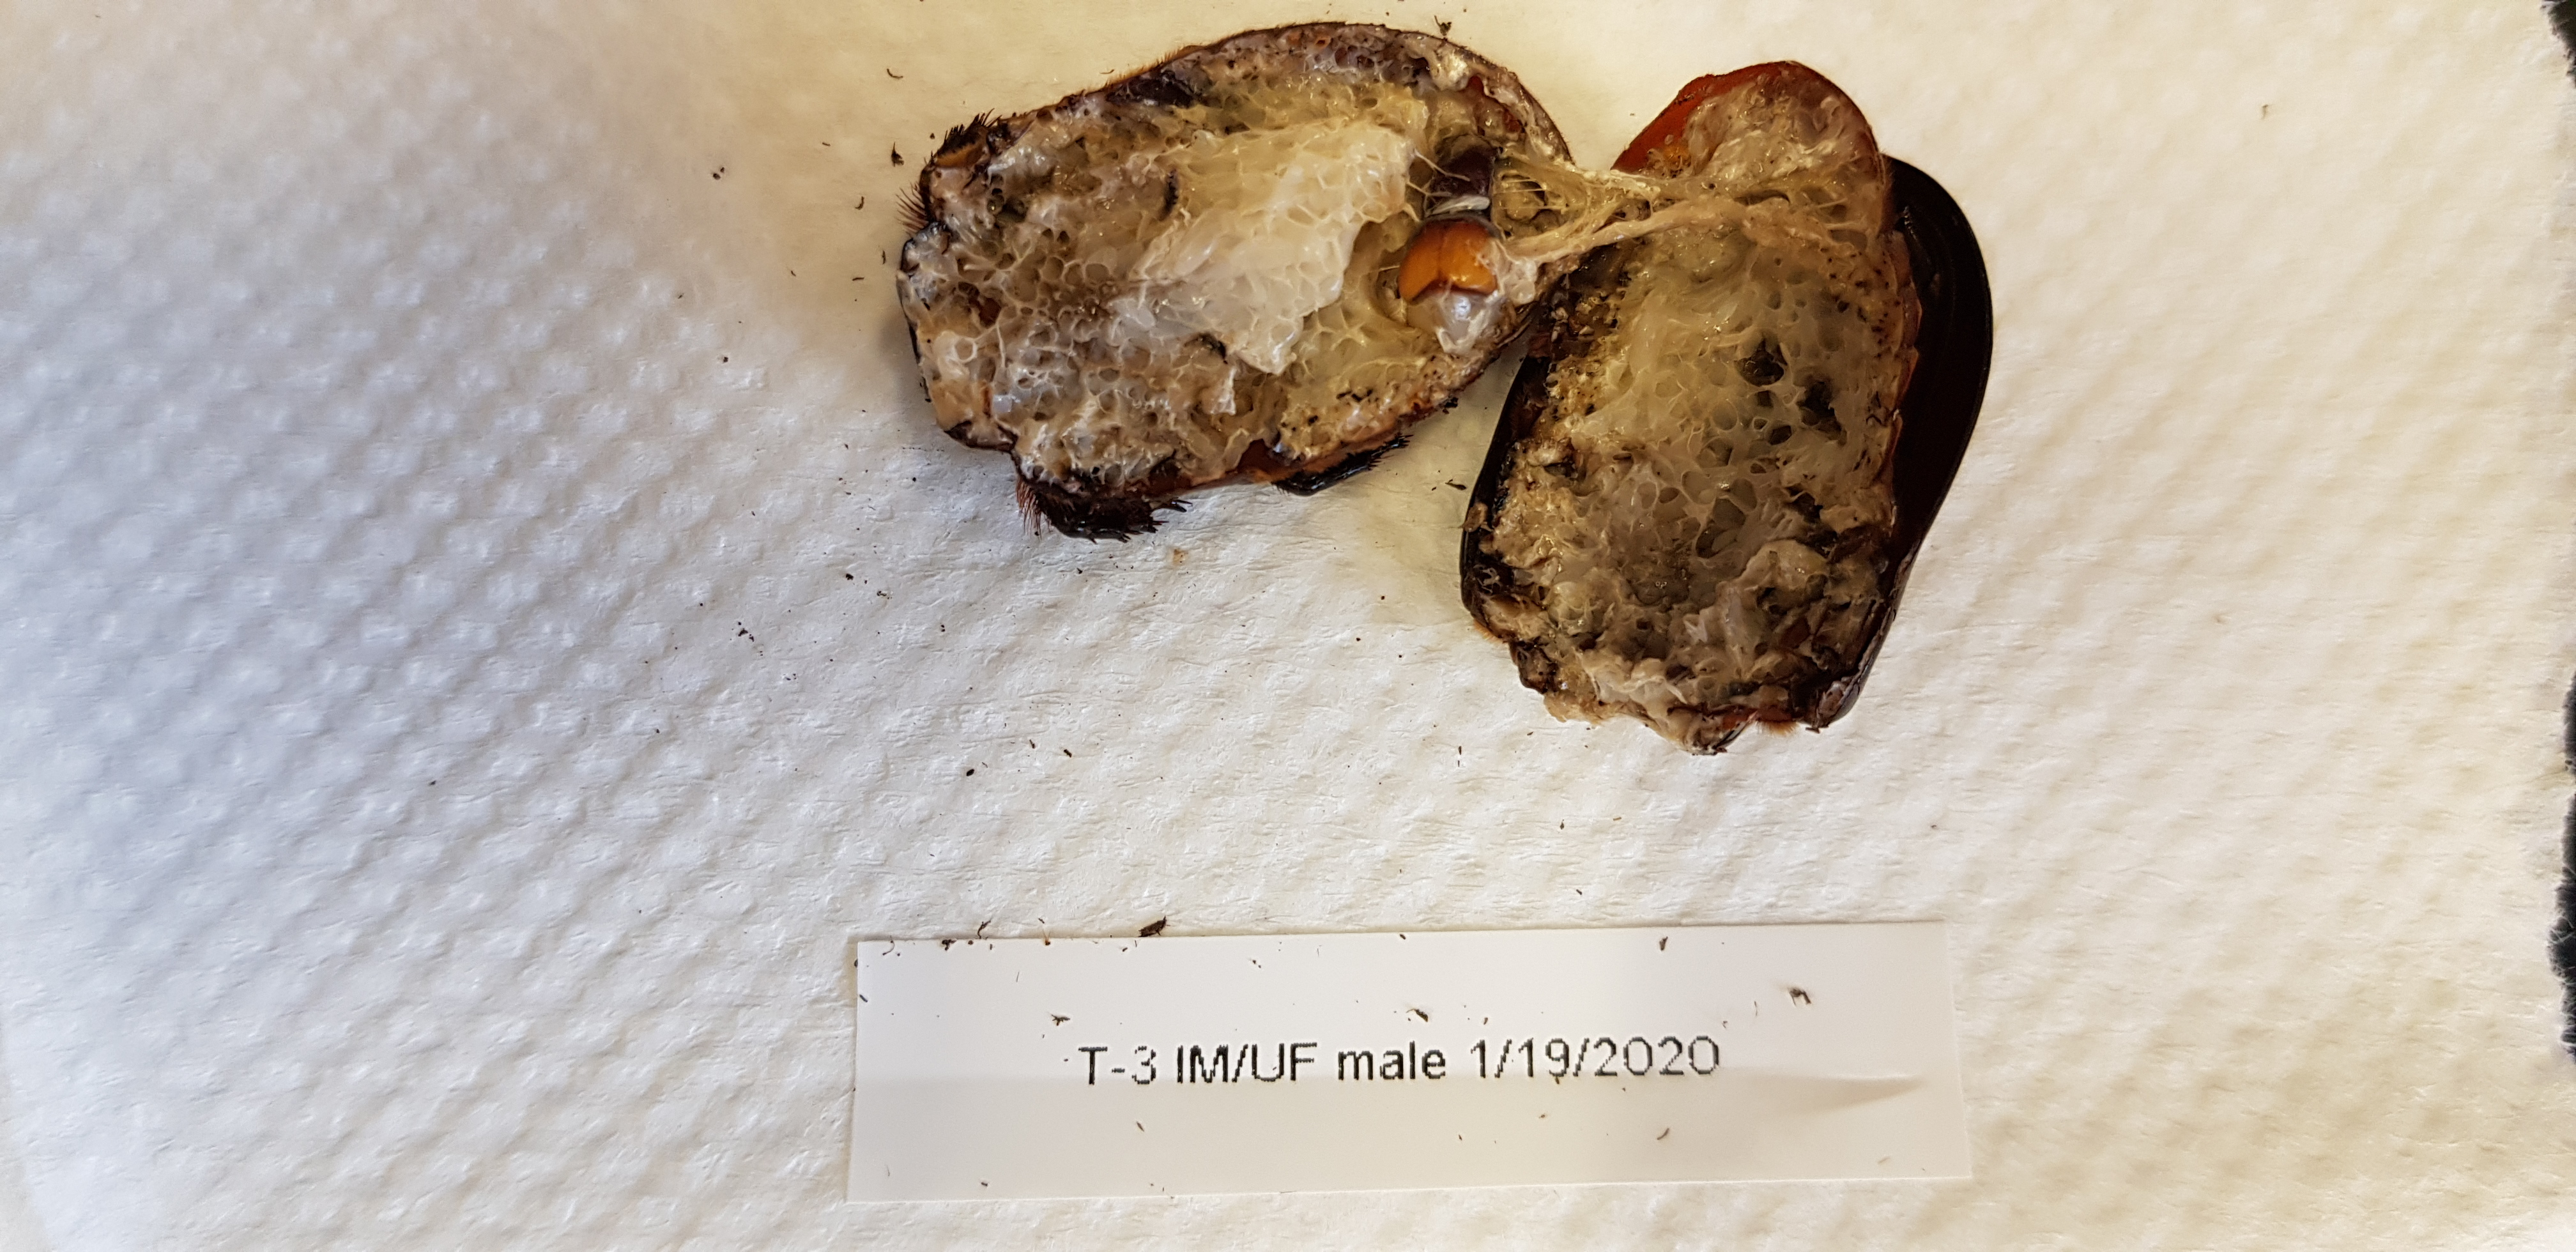
\includegraphics[width=\textwidth]{pm-images/20200119_122916.jpg}
\caption{\textbf{TM3m} jar\_id                                 TM3
sex                                      m
treatment                            virus
date\_treated           2019-12-26 00:00:00
date\_died              2020-01-19 00:00:00
postmortem\_virus                       NaN
postmortem\_bacteria                    NaN
pm\_image\_filename      20200119\_122916.jpg
date\_end\_bioassay      2020-02-06 00:00:00
t                                       24
e                                     True
Name: 62, dtype: object}
\end{figure}
\clearpage

\begin{figure}[h!]
\centering
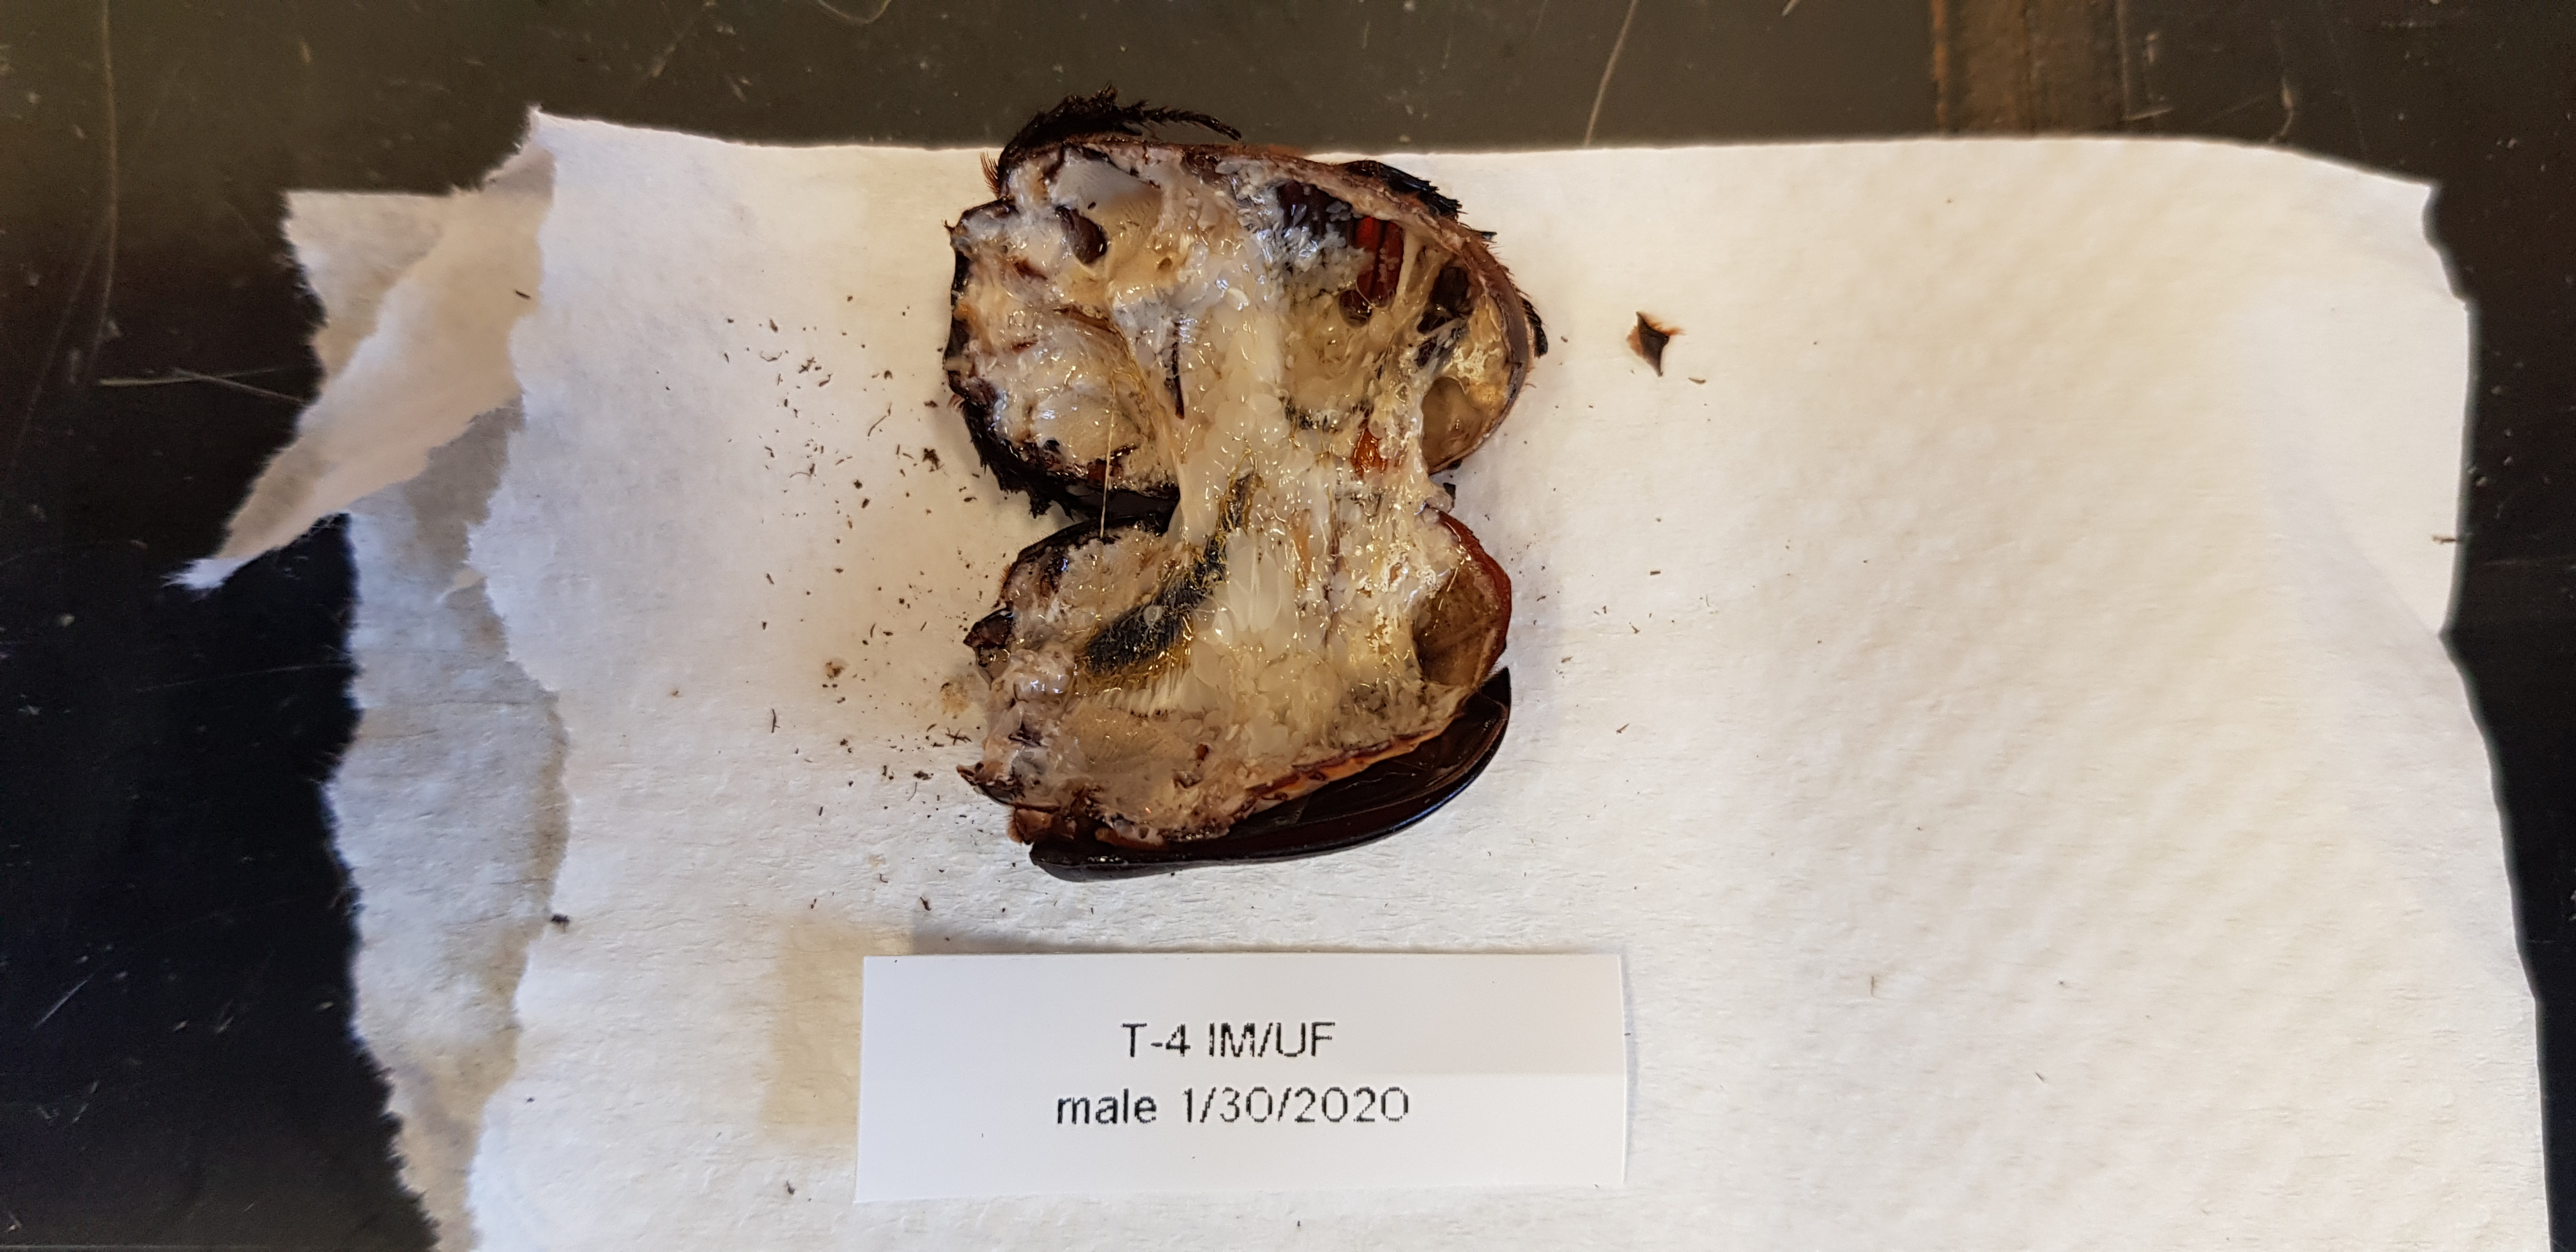
\includegraphics[width=\textwidth]{pm-images/20200131_115718.jpg}
\caption{\textbf{TM4m} jar\_id                                 TM4
sex                                      m
treatment                            virus
date\_treated           2019-12-26 00:00:00
date\_died              2020-01-31 00:00:00
postmortem\_virus                       NaN
postmortem\_bacteria                    NaN
pm\_image\_filename      20200131\_115718.jpg
date\_end\_bioassay      2020-02-06 00:00:00
t                                       36
e                                     True
Name: 63, dtype: object}
\end{figure}
\clearpage

\begin{figure}[h!]
\centering
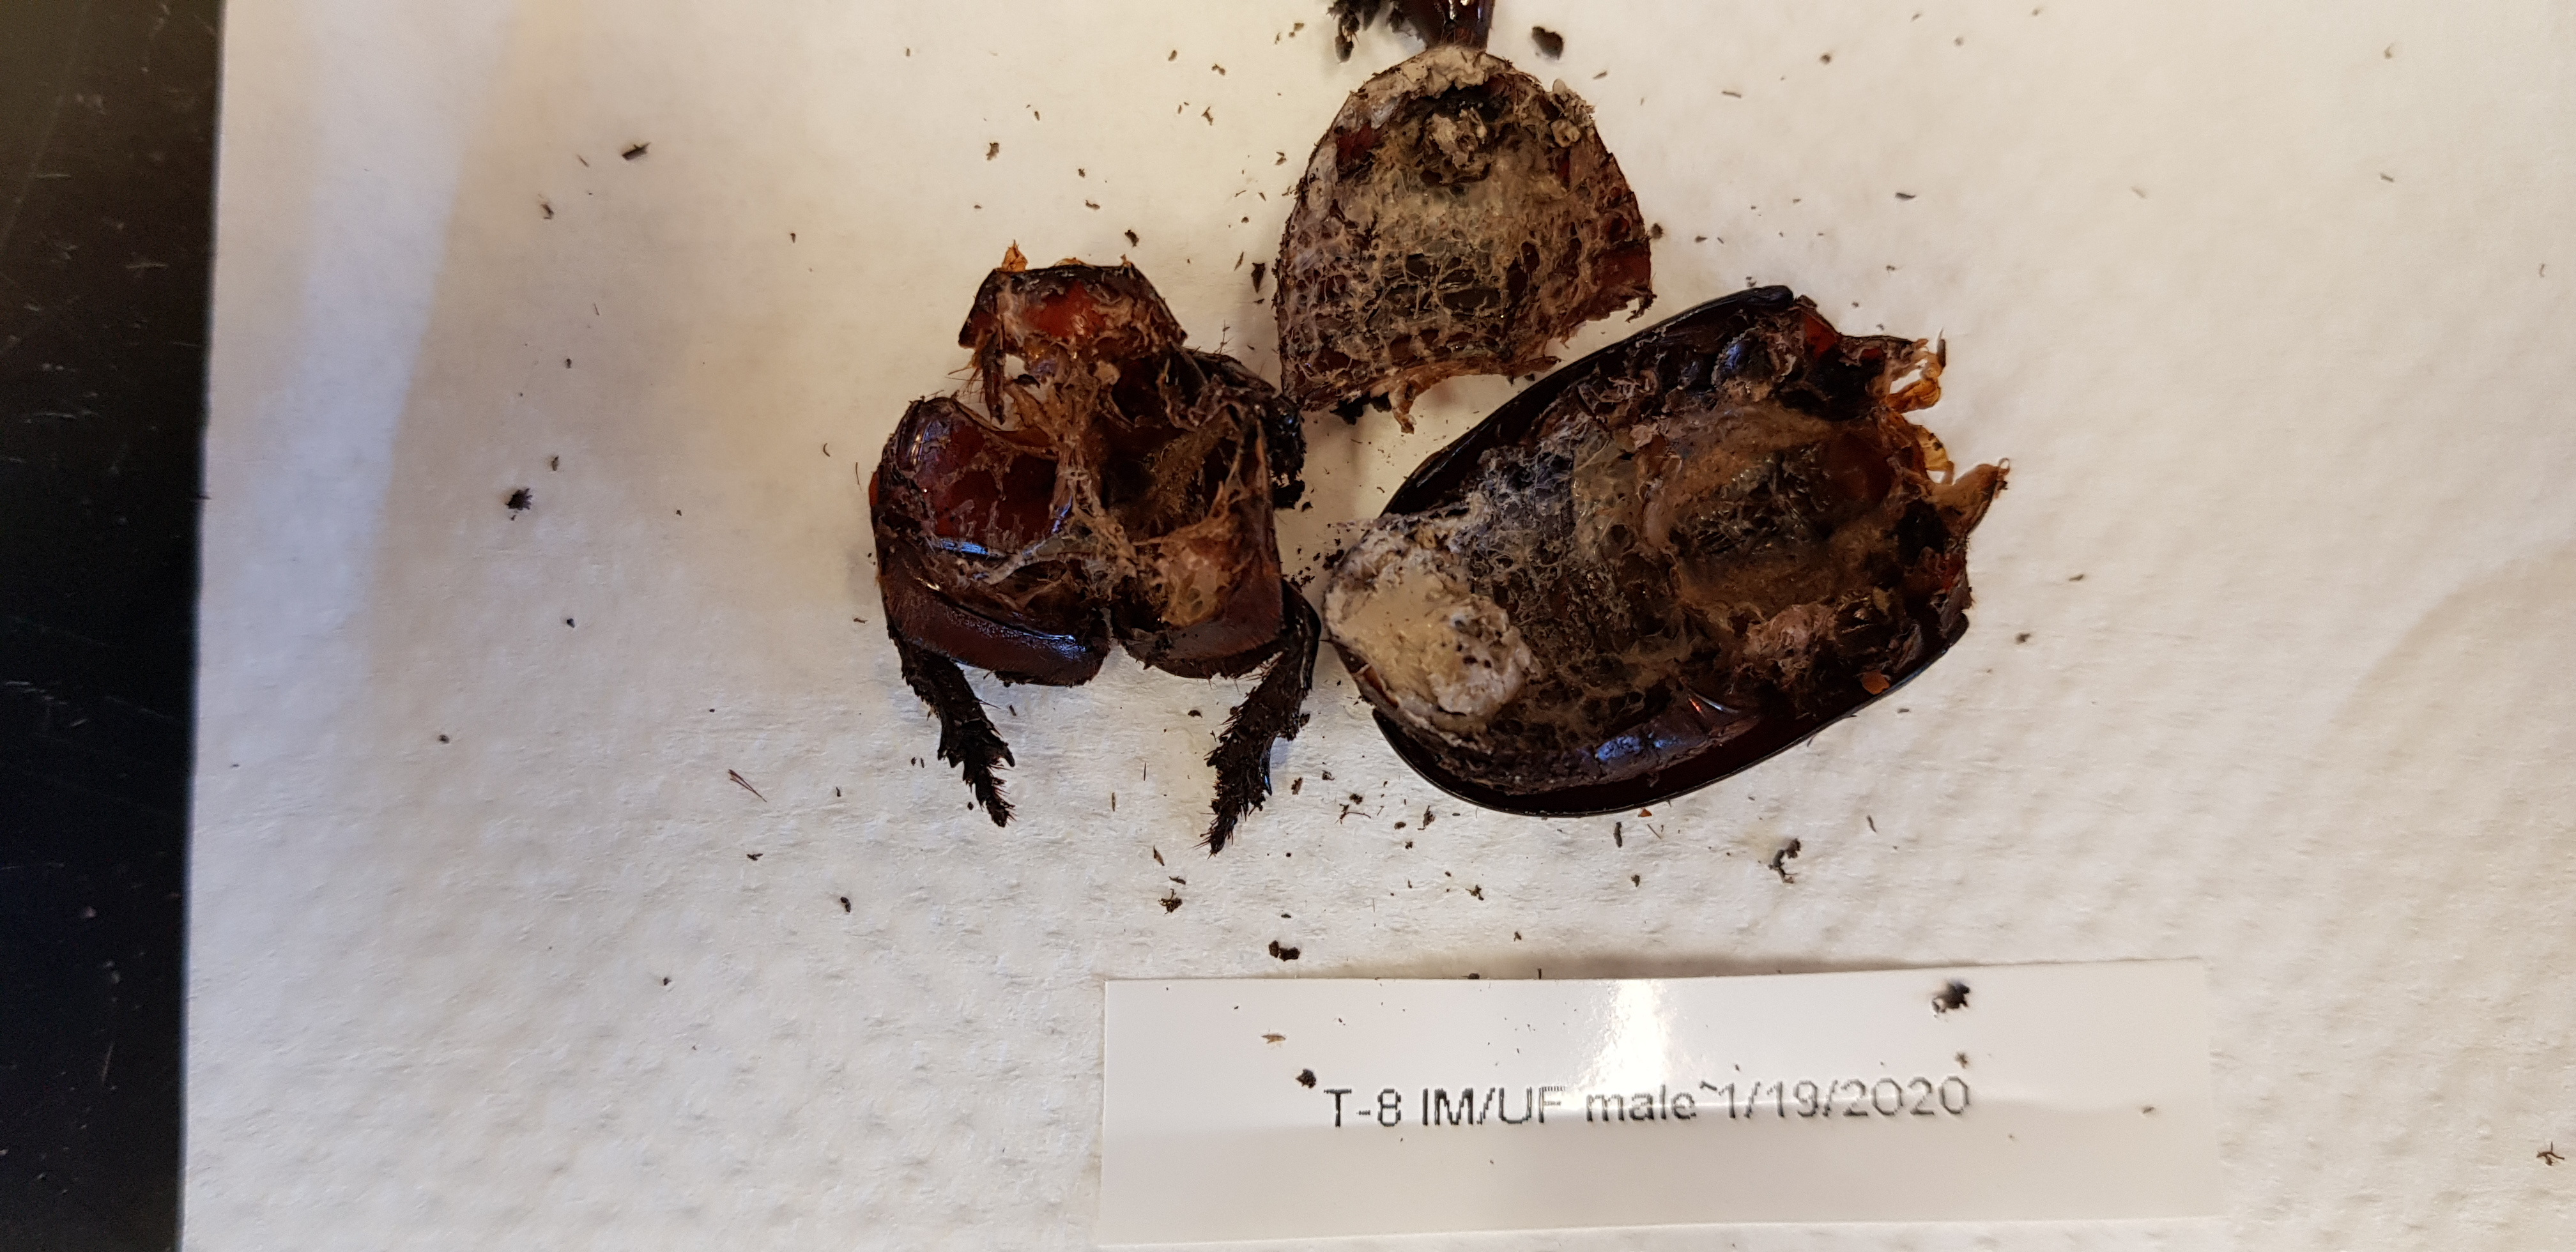
\includegraphics[width=\textwidth]{pm-images/20200119_115644.jpg}
\caption{\textbf{TM8m} jar\_id                                 TM8
sex                                      m
treatment                            virus
date\_treated           2019-12-27 00:00:00
date\_died              2020-01-19 00:00:00
postmortem\_virus                       NaN
postmortem\_bacteria                    NaN
pm\_image\_filename      20200119\_115644.jpg
date\_end\_bioassay      2020-02-06 00:00:00
t                                       23
e                                     True
Name: 67, dtype: object}
\end{figure}
\clearpage

\begin{figure}[h!]
\centering
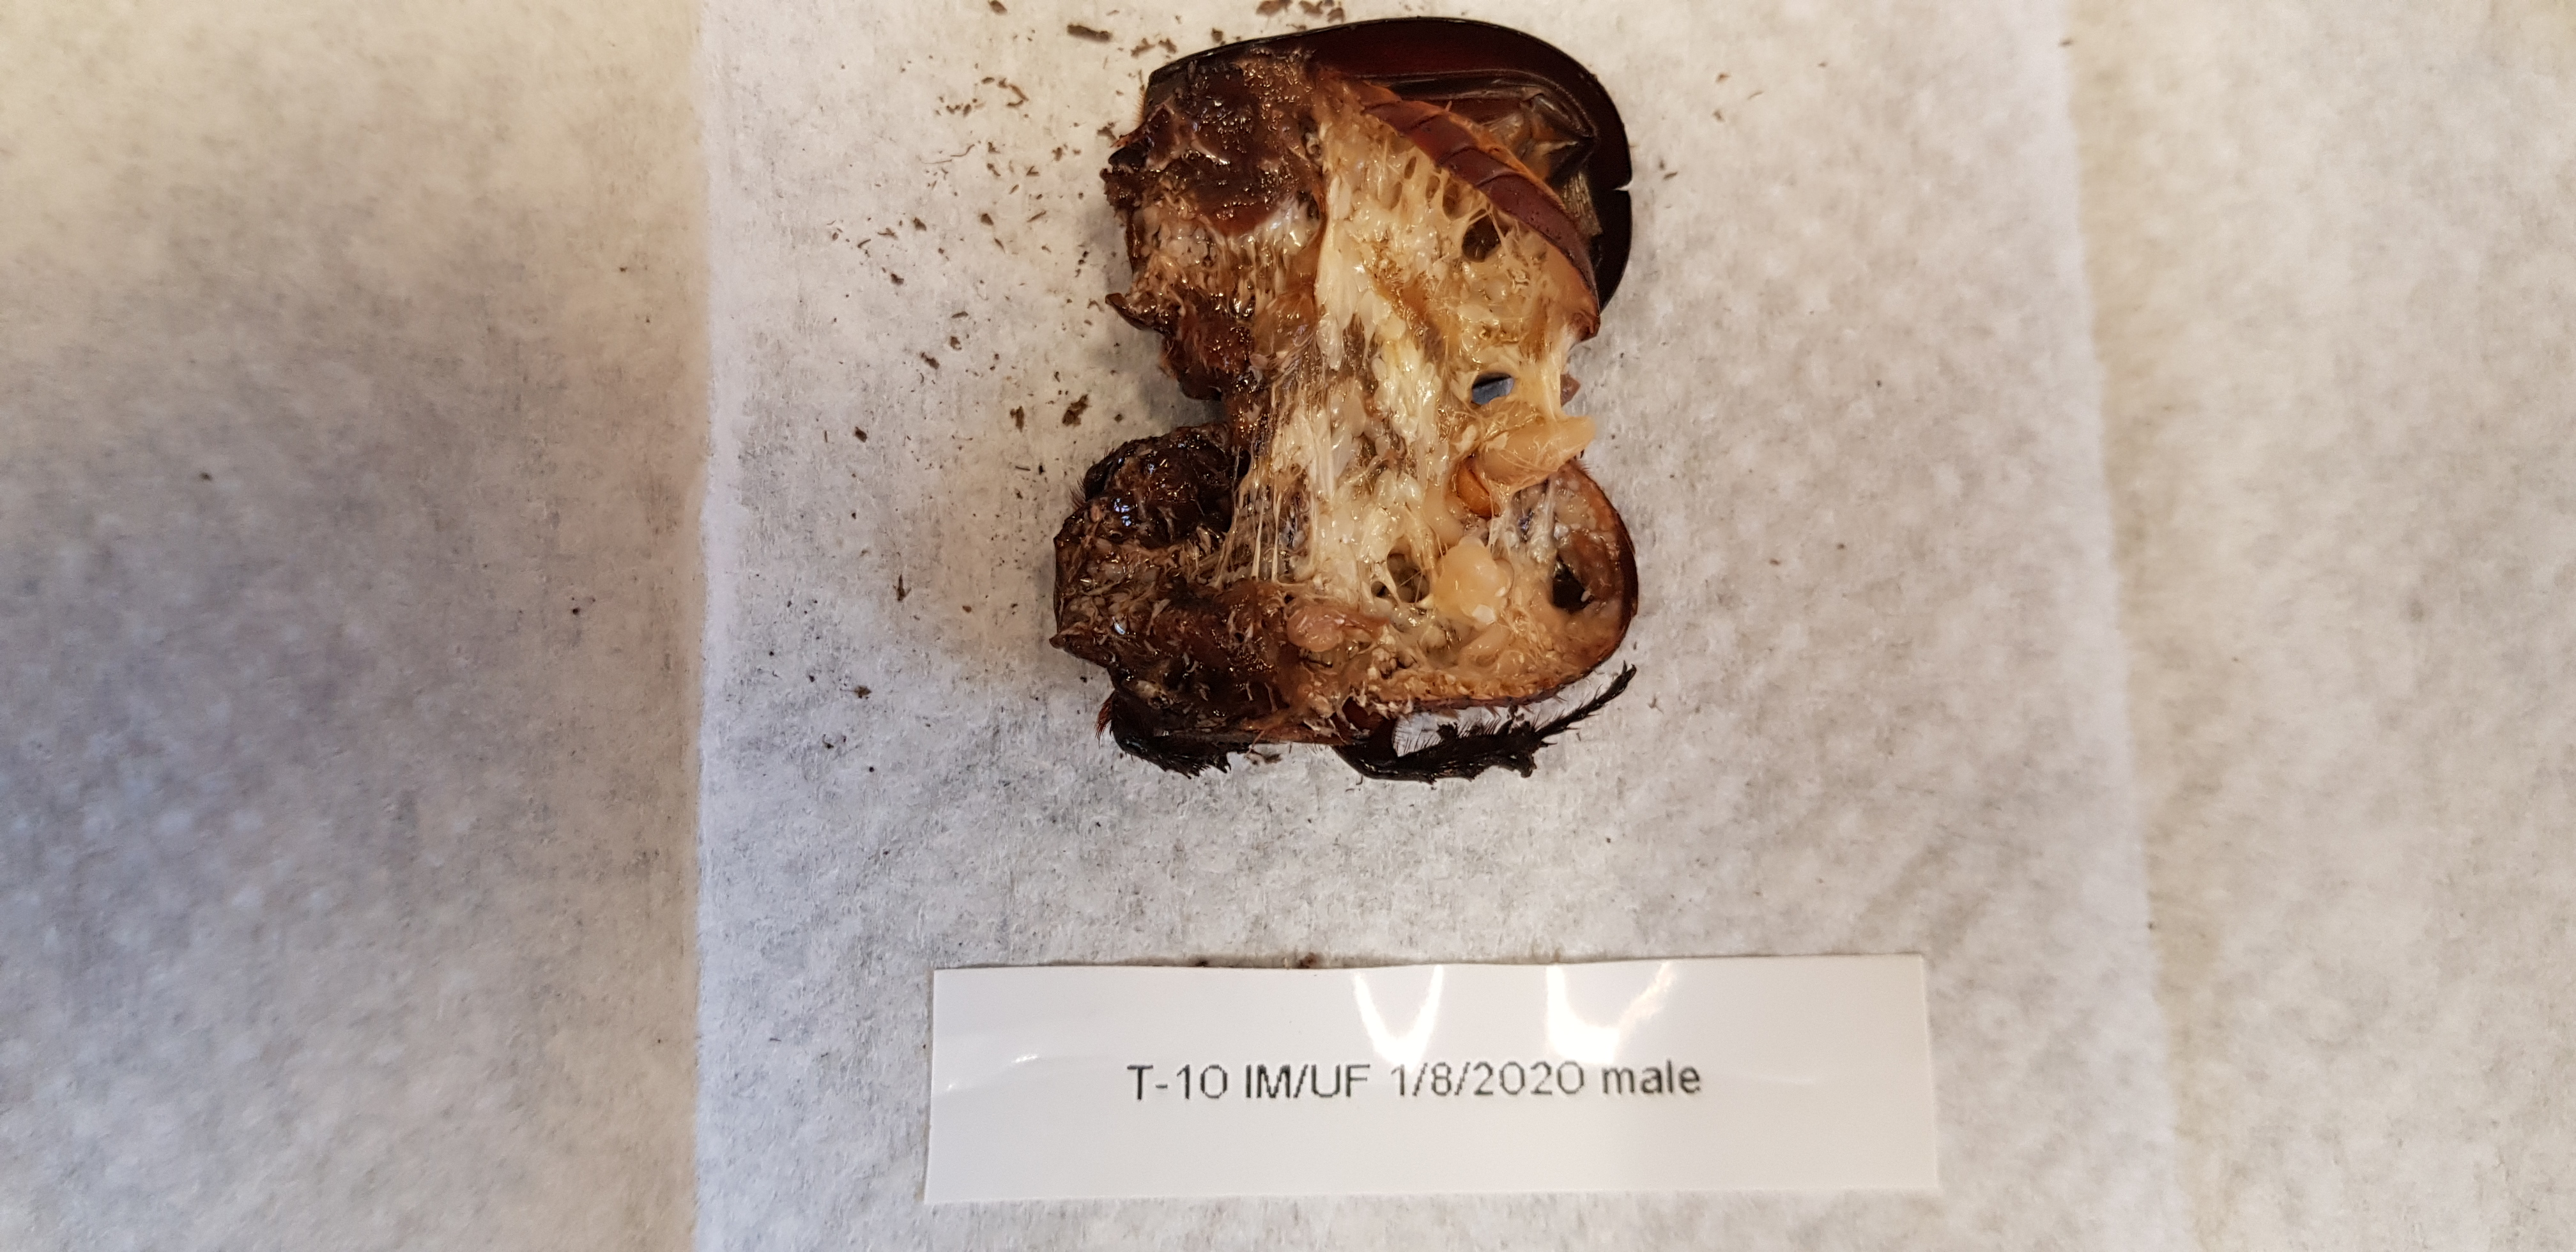
\includegraphics[width=\textwidth]{pm-images/20200108_102337.jpg}
\caption{\textbf{TM10m} jar\_id                                TM10
sex                                      m
treatment                            virus
date\_treated           2019-12-27 00:00:00
date\_died              2020-01-08 00:00:00
postmortem\_virus                         1
postmortem\_bacteria                      1
pm\_image\_filename      20200108\_102337.jpg
date\_end\_bioassay      2020-02-06 00:00:00
t                                       12
e                                     True
Name: 69, dtype: object}
\end{figure}
\clearpage

\begin{figure}[h!]
\centering
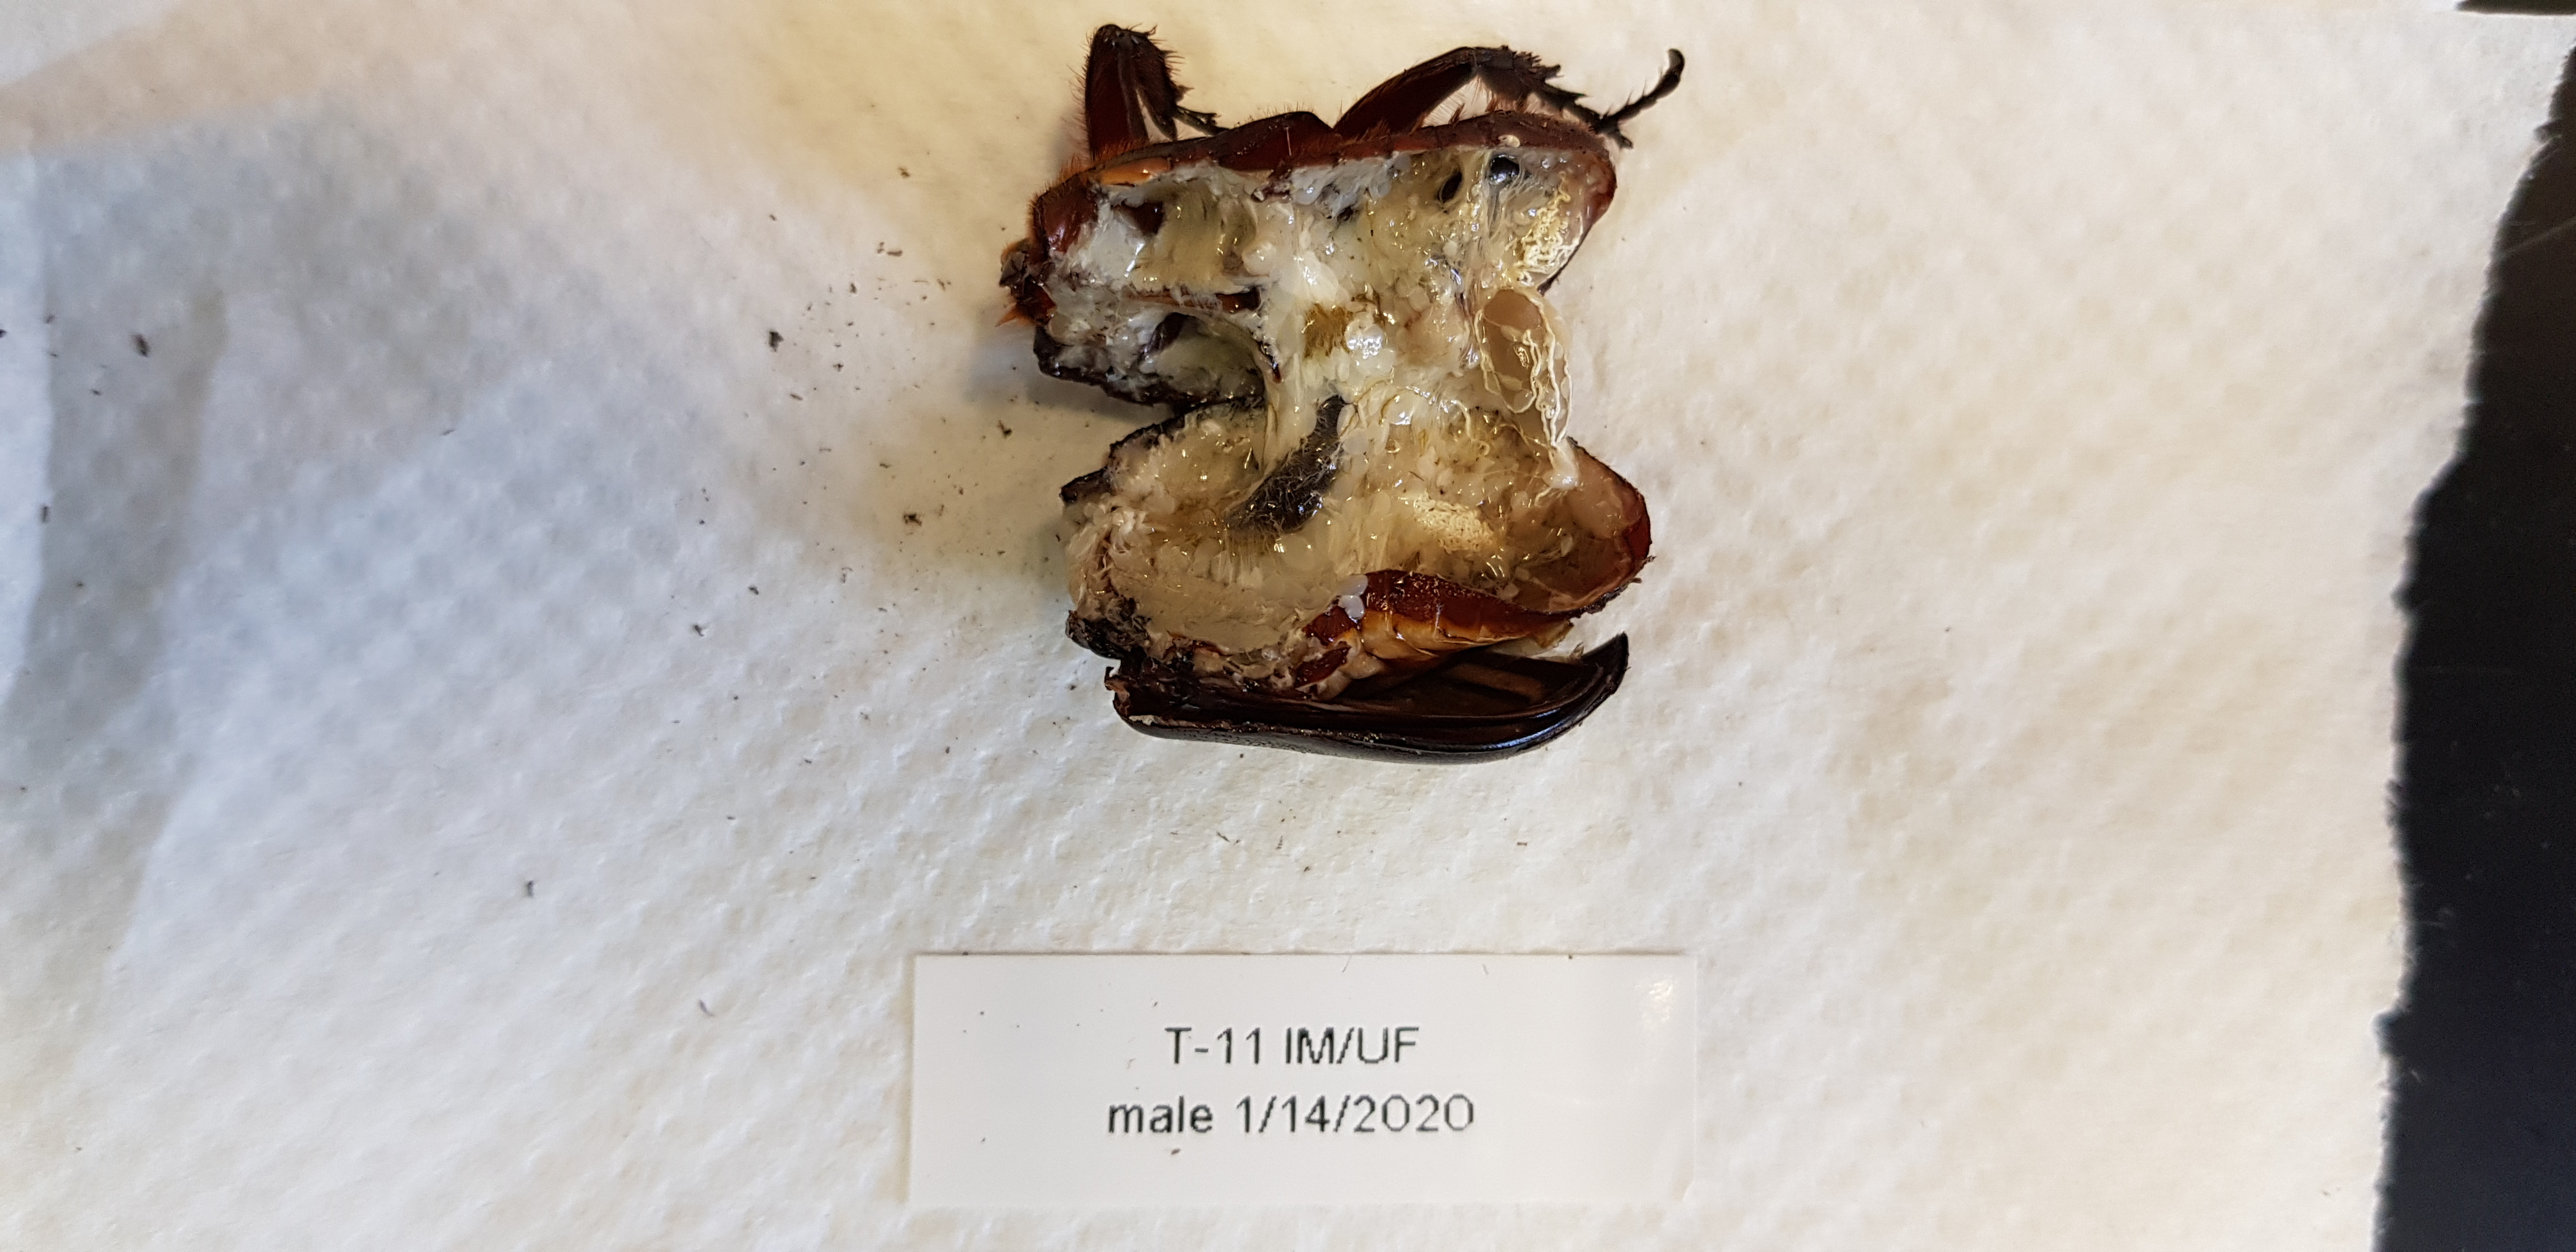
\includegraphics[width=\textwidth]{pm-images/20200114_105113.jpg}
\caption{\textbf{TM11m} jar\_id                                TM11
sex                                      m
treatment                            virus
date\_treated           2019-12-27 00:00:00
date\_died              2020-01-14 00:00:00
postmortem\_virus                       NaN
postmortem\_bacteria                    NaN
pm\_image\_filename      20200114\_105113.jpg
date\_end\_bioassay      2020-02-06 00:00:00
t                                       18
e                                     True
Name: 70, dtype: object}
\end{figure}
\clearpage

\begin{figure}[h!]
\centering
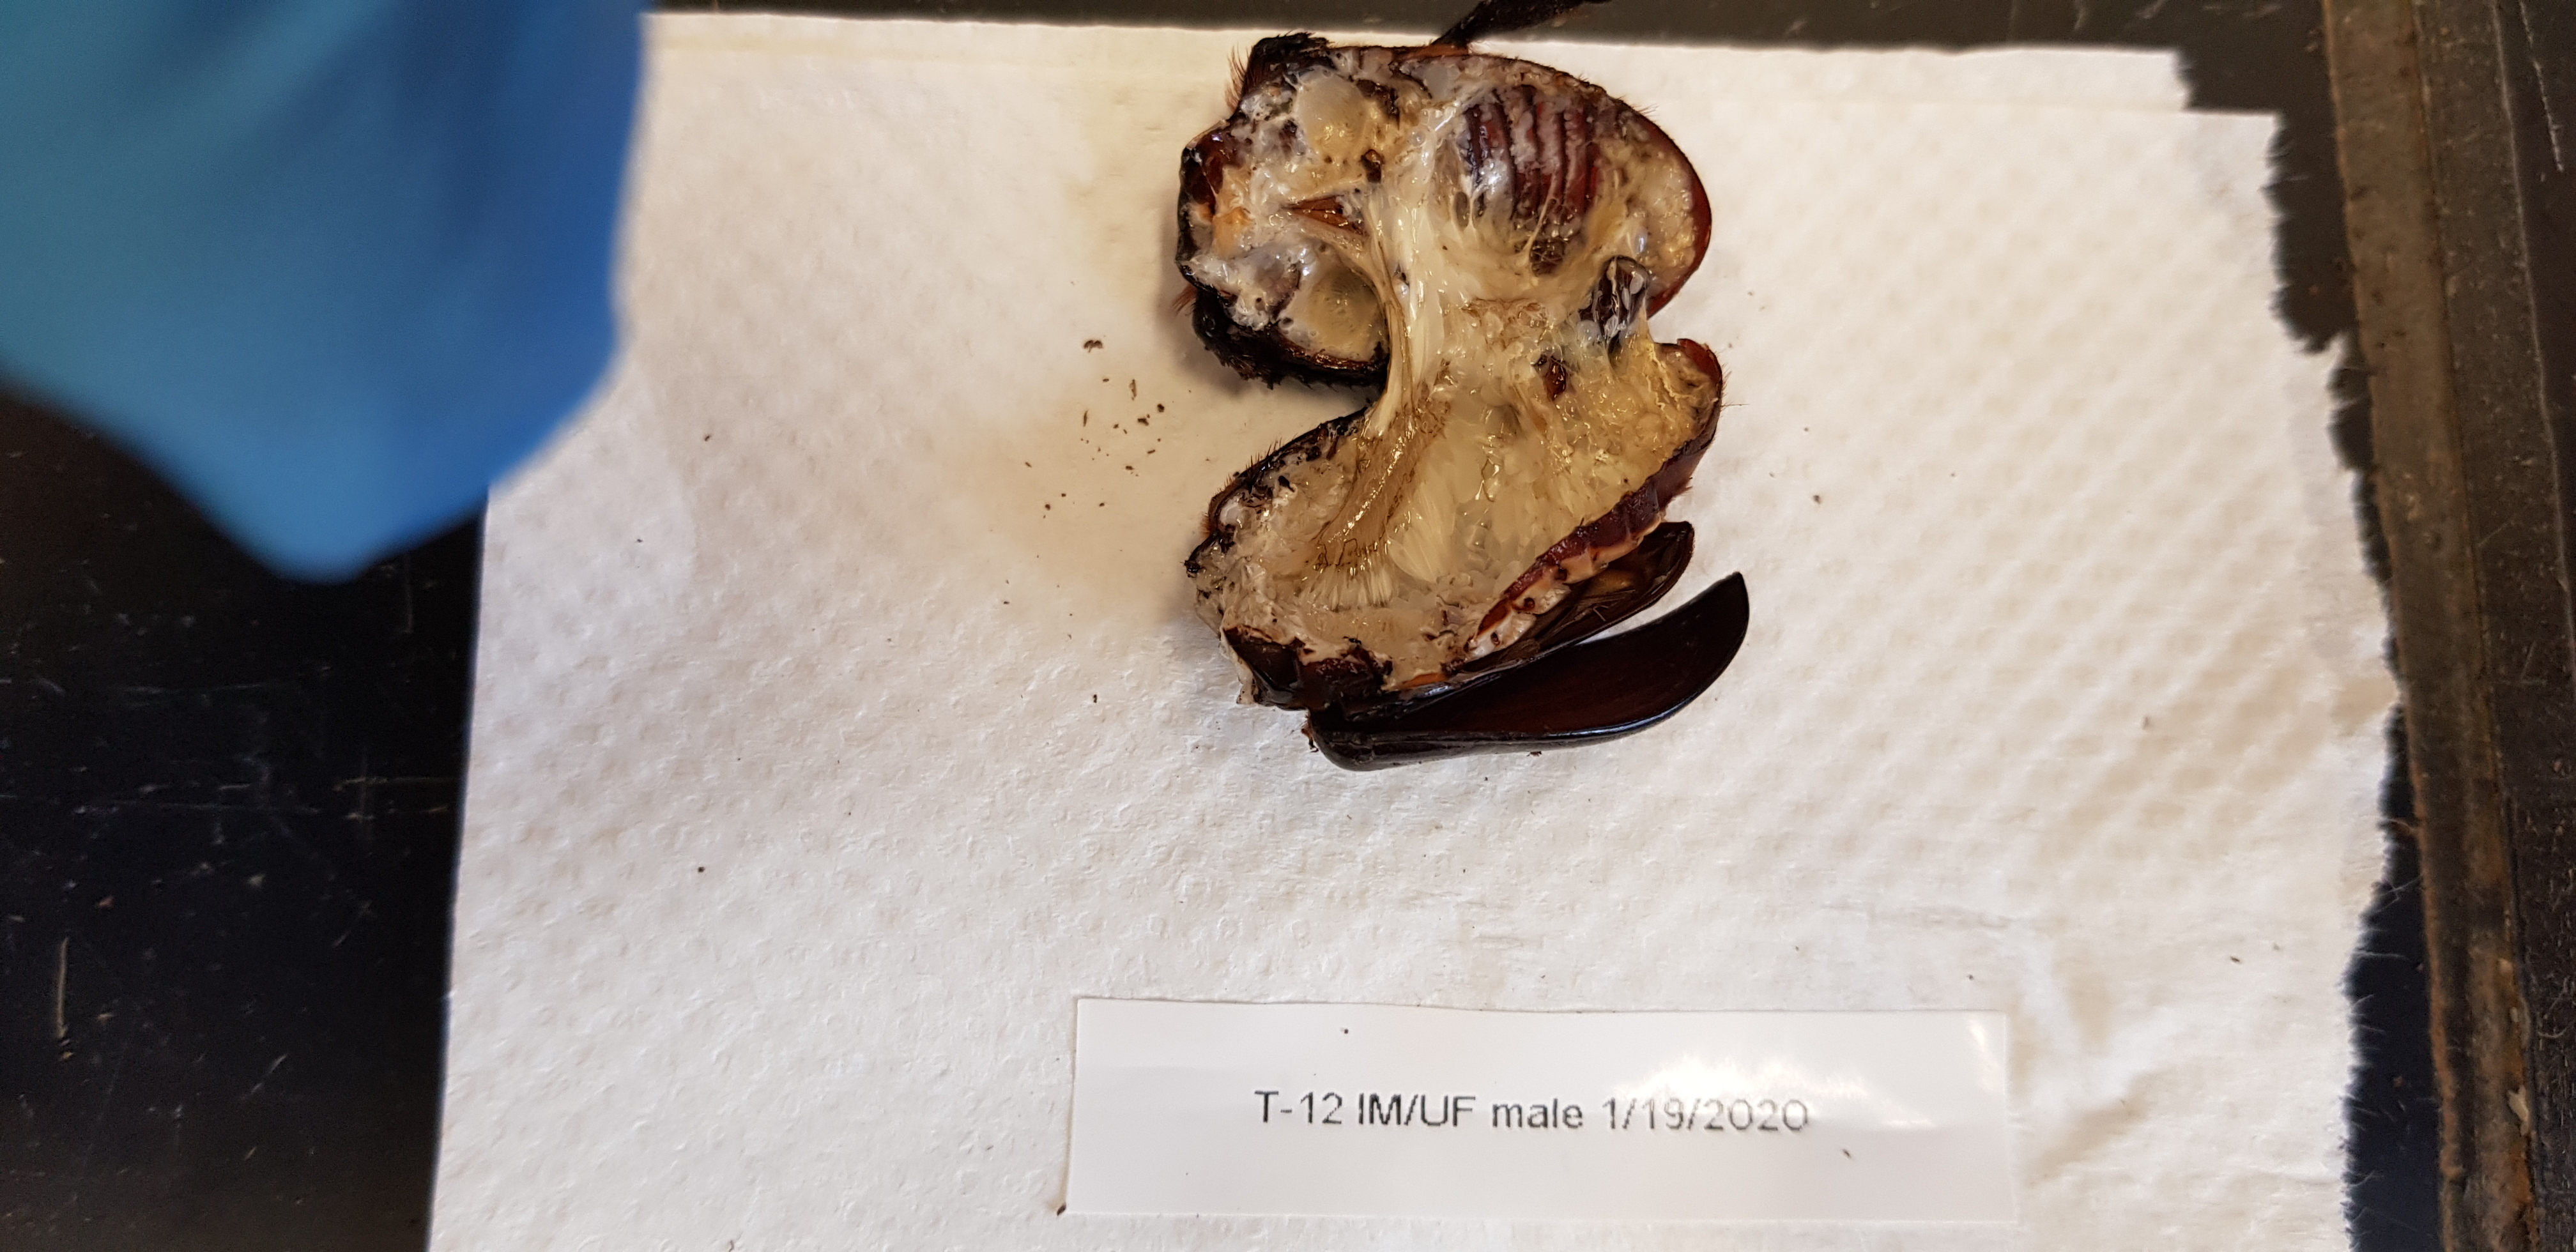
\includegraphics[width=\textwidth]{pm-images/20200119_122428.jpg}
\caption{\textbf{TM12m} jar\_id                                TM12
sex                                      m
treatment                            virus
date\_treated           2019-12-27 00:00:00
date\_died              2020-01-19 00:00:00
postmortem\_virus                       NaN
postmortem\_bacteria                    NaN
pm\_image\_filename      20200119\_122428.jpg
date\_end\_bioassay      2020-02-06 00:00:00
t                                       23
e                                     True
Name: 71, dtype: object}
\end{figure}
\clearpage

\begin{figure}[h!]
\centering
\includegraphics[width=\textwidth]{pm-images/20200129_152333.jpg}
\caption{\textbf{TM13m} jar\_id                                TM13
sex                                      m
treatment                            virus
date\_treated           2019-12-27 00:00:00
date\_died              2020-01-29 00:00:00
postmortem\_virus                       NaN
postmortem\_bacteria                    NaN
pm\_image\_filename      20200129\_152333.jpg
date\_end\_bioassay      2020-02-06 00:00:00
t                                       33
e                                     True
Name: 72, dtype: object}
\end{figure}
\clearpage

\begin{figure}[h!]
\centering
\includegraphics[width=\textwidth]{pm-images/20200129_154608.jpg}
\caption{\textbf{TM14m} jar\_id                                TM14
sex                                      m
treatment                            virus
date\_treated           2019-12-27 00:00:00
date\_died              2020-01-29 00:00:00
postmortem\_virus                       NaN
postmortem\_bacteria                    NaN
pm\_image\_filename      20200129\_154608.jpg
date\_end\_bioassay      2020-02-06 00:00:00
t                                       33
e                                     True
Name: 73, dtype: object}
\end{figure}
\clearpage

\begin{figure}[h!]
\centering
\includegraphics[width=\textwidth]{pm-images/20200127_150141.jpg}
\caption{\textbf{TM2f} jar\_id                                 TM2
sex                                      f
treatment                        companion
date\_treated           2019-12-26 00:00:00
date\_died              2020-01-27 00:00:00
postmortem\_virus                       NaN
postmortem\_bacteria                    NaN
pm\_image\_filename      20200127\_150141.jpg
date\_end\_bioassay      2020-02-06 00:00:00
t                                       32
e                                     True
Name: 76, dtype: object}
\end{figure}
\clearpage

\begin{figure}[h!]
\centering
\includegraphics[width=\textwidth]{pm-images/20200206_113320.jpg}
\caption{\textbf{TM3f} jar\_id                                 TM3
sex                                      f
treatment                        companion
date\_treated           2019-12-26 00:00:00
date\_died              2020-02-06 00:00:00
postmortem\_virus                       NaN
postmortem\_bacteria                    NaN
pm\_image\_filename      20200206\_113320.jpg
date\_end\_bioassay      2020-02-06 00:00:00
t                                       42
e                                     True
Name: 77, dtype: object}
\end{figure}
\clearpage

\begin{figure}[h!]
\centering
\includegraphics[width=\textwidth]{pm-images/20200119_124629.jpg}
\caption{\textbf{TM5f} jar\_id                                 TM5
sex                                      f
treatment                        companion
date\_treated           2019-12-26 00:00:00
date\_died              2020-01-19 00:00:00
postmortem\_virus                       NaN
postmortem\_bacteria                    NaN
pm\_image\_filename      20200119\_124629.jpg
date\_end\_bioassay      2020-02-06 00:00:00
t                                       24
e                                     True
Name: 79, dtype: object}
\end{figure}
\clearpage

\begin{figure}[h!]
\centering
\includegraphics[width=\textwidth]{pm-images/20200108_103227.jpg}
\caption{\textbf{TM8f} jar\_id                                 TM8
sex                                      f
treatment                        companion
date\_treated           2019-12-27 00:00:00
date\_died              2020-02-06 00:00:00
postmortem\_virus                       NaN
postmortem\_bacteria                    NaN
pm\_image\_filename      20200108\_103227.jpg
date\_end\_bioassay      2020-02-06 00:00:00
t                                       41
e                                     True
Name: 82, dtype: object}
\end{figure}
\clearpage

\begin{figure}[h!]
\centering
\includegraphics[width=\textwidth]{pm-images/20200114_105656.jpg}
\caption{\textbf{TM10f} jar\_id                                TM10
sex                                      f
treatment                        companion
date\_treated           2019-12-27 00:00:00
date\_died              2020-01-14 00:00:00
postmortem\_virus                       NaN
postmortem\_bacteria                      1
pm\_image\_filename      20200114\_105656.jpg
date\_end\_bioassay      2020-02-06 00:00:00
t                                       18
e                                     True
Name: 84, dtype: object}
\end{figure}
\clearpage

\begin{figure}[h!]
\centering
\includegraphics[width=\textwidth]{pm-images/20200129_152948.jpg}
\caption{\textbf{TM11f} jar\_id                                TM11
sex                                      f
treatment                        companion
date\_treated           2019-12-27 00:00:00
date\_died              2020-01-29 00:00:00
postmortem\_virus                       NaN
postmortem\_bacteria                    NaN
pm\_image\_filename      20200129\_152948.jpg
date\_end\_bioassay      2020-02-06 00:00:00
t                                       33
e                                     True
Name: 85, dtype: object}
\end{figure}
\clearpage

\begin{figure}[h!]
\centering
\includegraphics[width=\textwidth]{pm-images/20200203_113806.jpg}
\caption{\textbf{TM13f} jar\_id                                TM13
sex                                      f
treatment                        companion
date\_treated           2019-12-27 00:00:00
date\_died              2020-02-03 00:00:00
postmortem\_virus                       NaN
postmortem\_bacteria                    NaN
pm\_image\_filename      20200203\_113806.jpg
date\_end\_bioassay      2020-02-06 00:00:00
t                                       38
e                                     True
Name: 87, dtype: object}
\end{figure}
\clearpage

\begin{figure}[h!]
\centering
\includegraphics[width=\textwidth]{pm-images/20200114_104047.jpg}
\caption{\textbf{TM14f} jar\_id                                TM14
sex                                      f
treatment                        companion
date\_treated           2019-12-27 00:00:00
date\_died              2020-01-14 00:00:00
postmortem\_virus                       NaN
postmortem\_bacteria                    NaN
pm\_image\_filename      20200114\_104047.jpg
date\_end\_bioassay      2020-02-06 00:00:00
t                                       18
e                                     True
Name: 88, dtype: object}
\end{figure}
\clearpage

\begin{figure}[h!]
\centering
\includegraphics[width=\textwidth]{pm-images/20200119_120121.jpg}
\caption{\textbf{TM15f} jar\_id                                TM15
sex                                      f
treatment                        companion
date\_treated           2019-12-27 00:00:00
date\_died              2020-01-19 00:00:00
postmortem\_virus                       NaN
postmortem\_bacteria                    NaN
pm\_image\_filename      20200119\_120121.jpg
date\_end\_bioassay      2020-02-06 00:00:00
t                                       23
e                                     True
Name: 89, dtype: object}
\end{figure}
\clearpage


\clearpage

\end{document}

